\documentclass{report}
\title{WASC Self-Study Report}
\date{\today}
\author{CMIS}
\usepackage[a4paper, total={6in, 8in}]{geometry}
\usepackage{tabu,tabularx,colortbl,array}

\usepackage{fontspec}
\setmainfont{Times New Roman}

\usepackage[labelfont=bf]{caption}
\usepackage[table]{xcolor}
\usepackage{graphicx}
\graphicspath{ {images/} }
\usepackage{pdflscape}
\usepackage{multirow}
\usepackage{longtable}

\tabulinesep=^2pt_2pt
\usepackage{pgfplots}
%\usepackage{paracol}
\usepackage{blindtext}
%\usepackage{capt-of}
\usepackage{subfig}
\usepackage{enumitem}
\setlist{nosep}

\usepackage{anyfontsize}
\usepackage{verbatim}
\usepackage[explicit]{titlesec}
\usepackage{float}
\usepackage[export]{adjustbox}
\usepackage{wrapfig}
\floatstyle{boxed} 
\restylefloat{figure}
\usepackage{fancyhdr}
\pagestyle{fancy}
\fancyhf{}
\renewcommand{\headrulewidth}{0pt}
\cfoot{\thepage}
\chead{\leftmark}
\usepackage{xcolor}
\usepackage{tikz}
\setlength{\parskip}{1em}

\makeatletter
\ifnum\inputlineno=\m@ne
\let\showlineno\@empty
\else
\def\showlineno{\the\inputlineno}
\fi
\makeatother
\usepackage{float}
\floatstyle{plain}

\usepackage[most]{tcolorbox}
\usepackage{marginnote}
\usepackage{booktabs}
\newcommand{\debug}{%
        \marginnote{%
                \begin{debugBox}%
                        \jobname\showlineno%
                \end{debugBox}%
        }%
}

\newtcolorbox{evidenceBox}{%
  colback=black!5,
  colbacktitle=violet,
  boxrule=1pt,
  top=1em,
  breakable,
 % arc=4pt,
 % outer arc=4pt,
  title=Evidence
}

\newtcolorbox{findingsBox}{%
  colback=white,%black!5,
  colbacktitle=red,
  boxrule=1pt,
 % boxsep=1pt,
 % top=1em,%-0.5\baselineskip,
  breakable,
 % arc=4pt,
 % outer arc=4pt,
  title=Findings
}

\newtcolorbox{debugBox}{%
        colback=yellow,
        title=DEBUG
}
        

\newenvironment{findings}
{
\debug
\noindent\textbf{Findings}

}
{
%\end{findingsBox}
}

\newenvironment{evidence}
{
\debug
\begin{evidenceBox}
\vspace{-\topsep}
\begin{itemize}[leftmargin=*]
  \setlength{\parskip}{0pt}
  \setlength{\itemsep}{1pt}
}
{
\end{itemize}
\end{evidenceBox}
%\vspace{4em}
}


\newcommand{\indicator}[1]{ 
\noindent\textbf{Indicator:} #1
}

\newcommand{\prompt}[1]{ 
\noindent\textbf{Prompt:} \textit{#1}
}

\newenvironment{tbl}[2]
{
%\rowcolors{2}{lightgray}{white}
\tabularx{#1}{#2}
%\rowcolor{darkgray}
}
{
\endtabularx
}

%\usepackage{tocloft} 
%\setlength{\cftbeforetoctitleskip}{-5.5in}
%\renewcommand{\cfttoctitlefont}{\color{black}}
\usepackage{hyperref}
%\usepackage{scrreport}
%\renewcommand*{\chapterheadstartvskip}{\vspace*{0.75\textheight}}
\hypersetup{%
  pdftitle=WASC Self Report,
  colorlinks=true,
  urlcolor=blue,
  linkcolor=blue
  %urlbordercolor=magenta
}

\begin{document}
\newgeometry{left=0.5in, right=0pt,top=0pt,bottom=0pt}
\begin{titlepage}


\pagenumbering{gobble}
\centering


\vspace*{1in}

\begin{tabular}{cc}
\parbox[m]{0.2\textwidth}{
\includegraphics[width=0.2\textwidth]{CMIS_logo.png}} &
\parbox[m]{0.8\textwidth}{\raggedright\sffamily\bfseries\color{CmisPurple}{\fontsize{25}{30}\selectfont Chiang Mai International School} \\
\bigskip
{\Huge\color{black!50!CmisPurple}
Focus on Learning 

Self-Study Report}

\bigskip
WASC Accreditation Visit \\
March 19-23, 2017 \\
}\\%&
%\parbox[m]{0.3\textwidth}{
\includegraphics[width=0.20\textwidth]{CMIS_logo.png}} \\
\end{tabular}

\begin{tikzpicture}[remember picture, overlay]
\filldraw[fill=CmisPurple,draw=CmisPurple] (-12cm,-3) rectangle (10cm, -7);
\end{tikzpicture}

\bigskip

\AddToShipoutPicture*{\CoverPic{frontpage.jpg}}
\end{titlepage}
\pagenumbering{arabic}
\restoregeometry
%\maketitle
\tableofcontents
\clearpage

\chapter*{Preface}
\addcontentsline{toc}{chapter}{Preface}
\AddToShipoutPicture*{\BackgroundPic{title.jpg}}
\newpage

Chiang Mai International School (CMIS) is the oldest school in Chiang Mai and the third oldest international school in Thailand. Missionaries returning to work after World War II established the school for their seven children over sixty years ago. Today CMIS has grown into a diverse international school with over five hundred students originating from over thirty different countries. Despite the expansion, CMIS still promotes the values of Christianity, while warmly welcoming families of all faiths, cultures, and ethnicities. 

For over forty years, CMIS was the only international school in Chiang Mai. Today, international schools are numerous and CMIS remains a school of choice. With an emphasis on providing academic excellence, in a caring community, CMIS students grow to be confident, articulate learners as well as caring, globally-minded individuals. This commitment has resulted in CMIS being known to many as the best international school in Chiang Mai. This well-deserved reputation is evident in our inspiring students that continue to excel in many areas including the arts, athletics, academics, community service, and leadership. 

The CMIS Focus on Learning Self-Study report is the result of several years of collective action, coupled with times of reflection and discussion with teachers, students, staff, parents, and community members. Though the immediate staff and leadership contributed to the construction of the report, CMIS appreciates and honors the work of prior staff and administrative teams. 

\begin{figure}[h!]
\centering
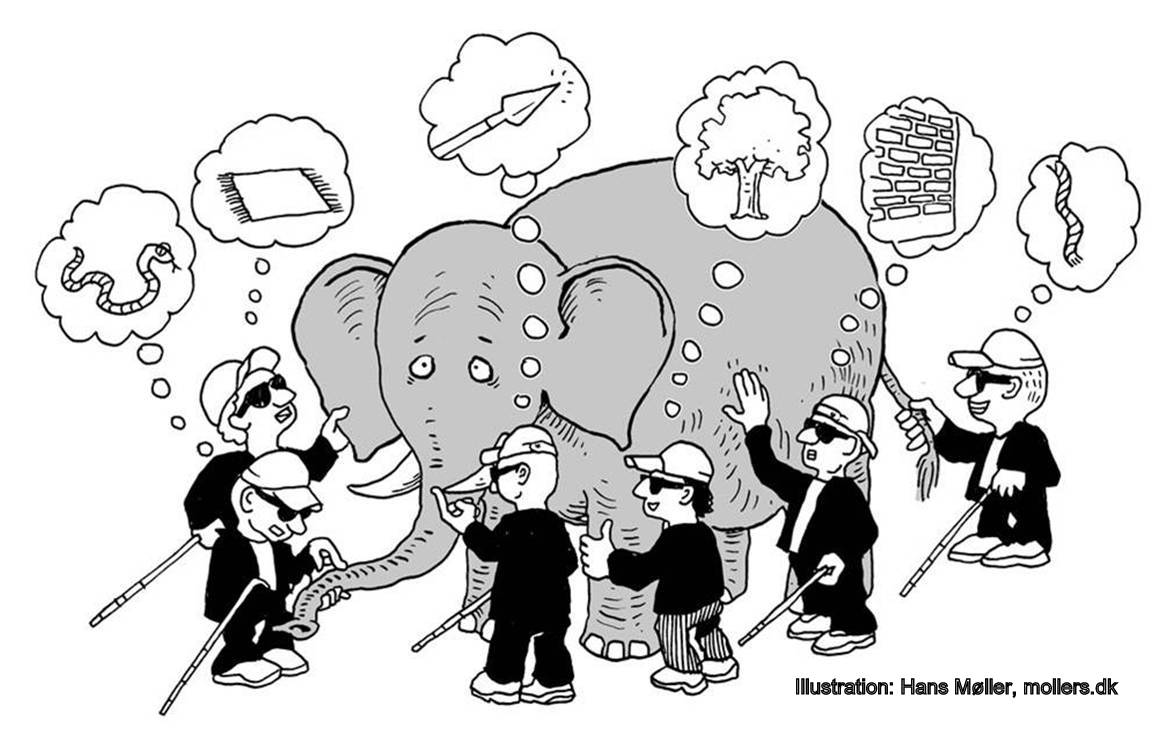
\includegraphics[width=\textwidth]{preface1.jpg}
\caption{Visual Analogy}
\label{figure:analogy}
\end{figure}

CMIS chose the visual parable based on the Indian story entitled Blind Men and the Elephant as the self-study mantra (see Figure \ref{figure:analogy}. In the story, a group of blind men touch an elephant to learn what it is like. Each one feels a different part, but only one part, such as the side or the tusk. They then compare notes and learn that they are in complete disagreement. The parable reminded CMIS of the importance of considering all viewpoints in obtaining a full picture of reality, and that our perceptions and life experiences can lead to limited access and overreaching misinterpretations. It was a poignant story for CMIS because in the past there had been times when parts of the school were working in isolation of one another. It helped CMIS to continuously focus on creating all the pieces of the report together, no matter how discreet, to best describe the whole. 

CMIS believes the primary goal of the report is to identify, articulate, and celebrate what CMIS already does to address its most essential institutional goal: to increase student learning. This was made clear, early in the self-study process, when a staff member suggested that the title of the report was Focus on Learning and that all of our reflections and discussions should be anchored to that idea. From that point forward, CMIS referred to the WASC process and construction of the report as the Focus on Learning. 

An overview and summary given by WASC consultant Barbara Parker officially inaugurated the development of focus and home groups and the collection of self-study data in November 2016. This presentation reminded the CMIS team see the report as a valuable self-evaluation tool. Focus on Learning should not be seen as an additional task, only referred to during the accreditation year, but rather as a protocol that guides schools into an ongoing improvement process that includes implementation, assessment, and refinement of the schoolwide planning.

{\centering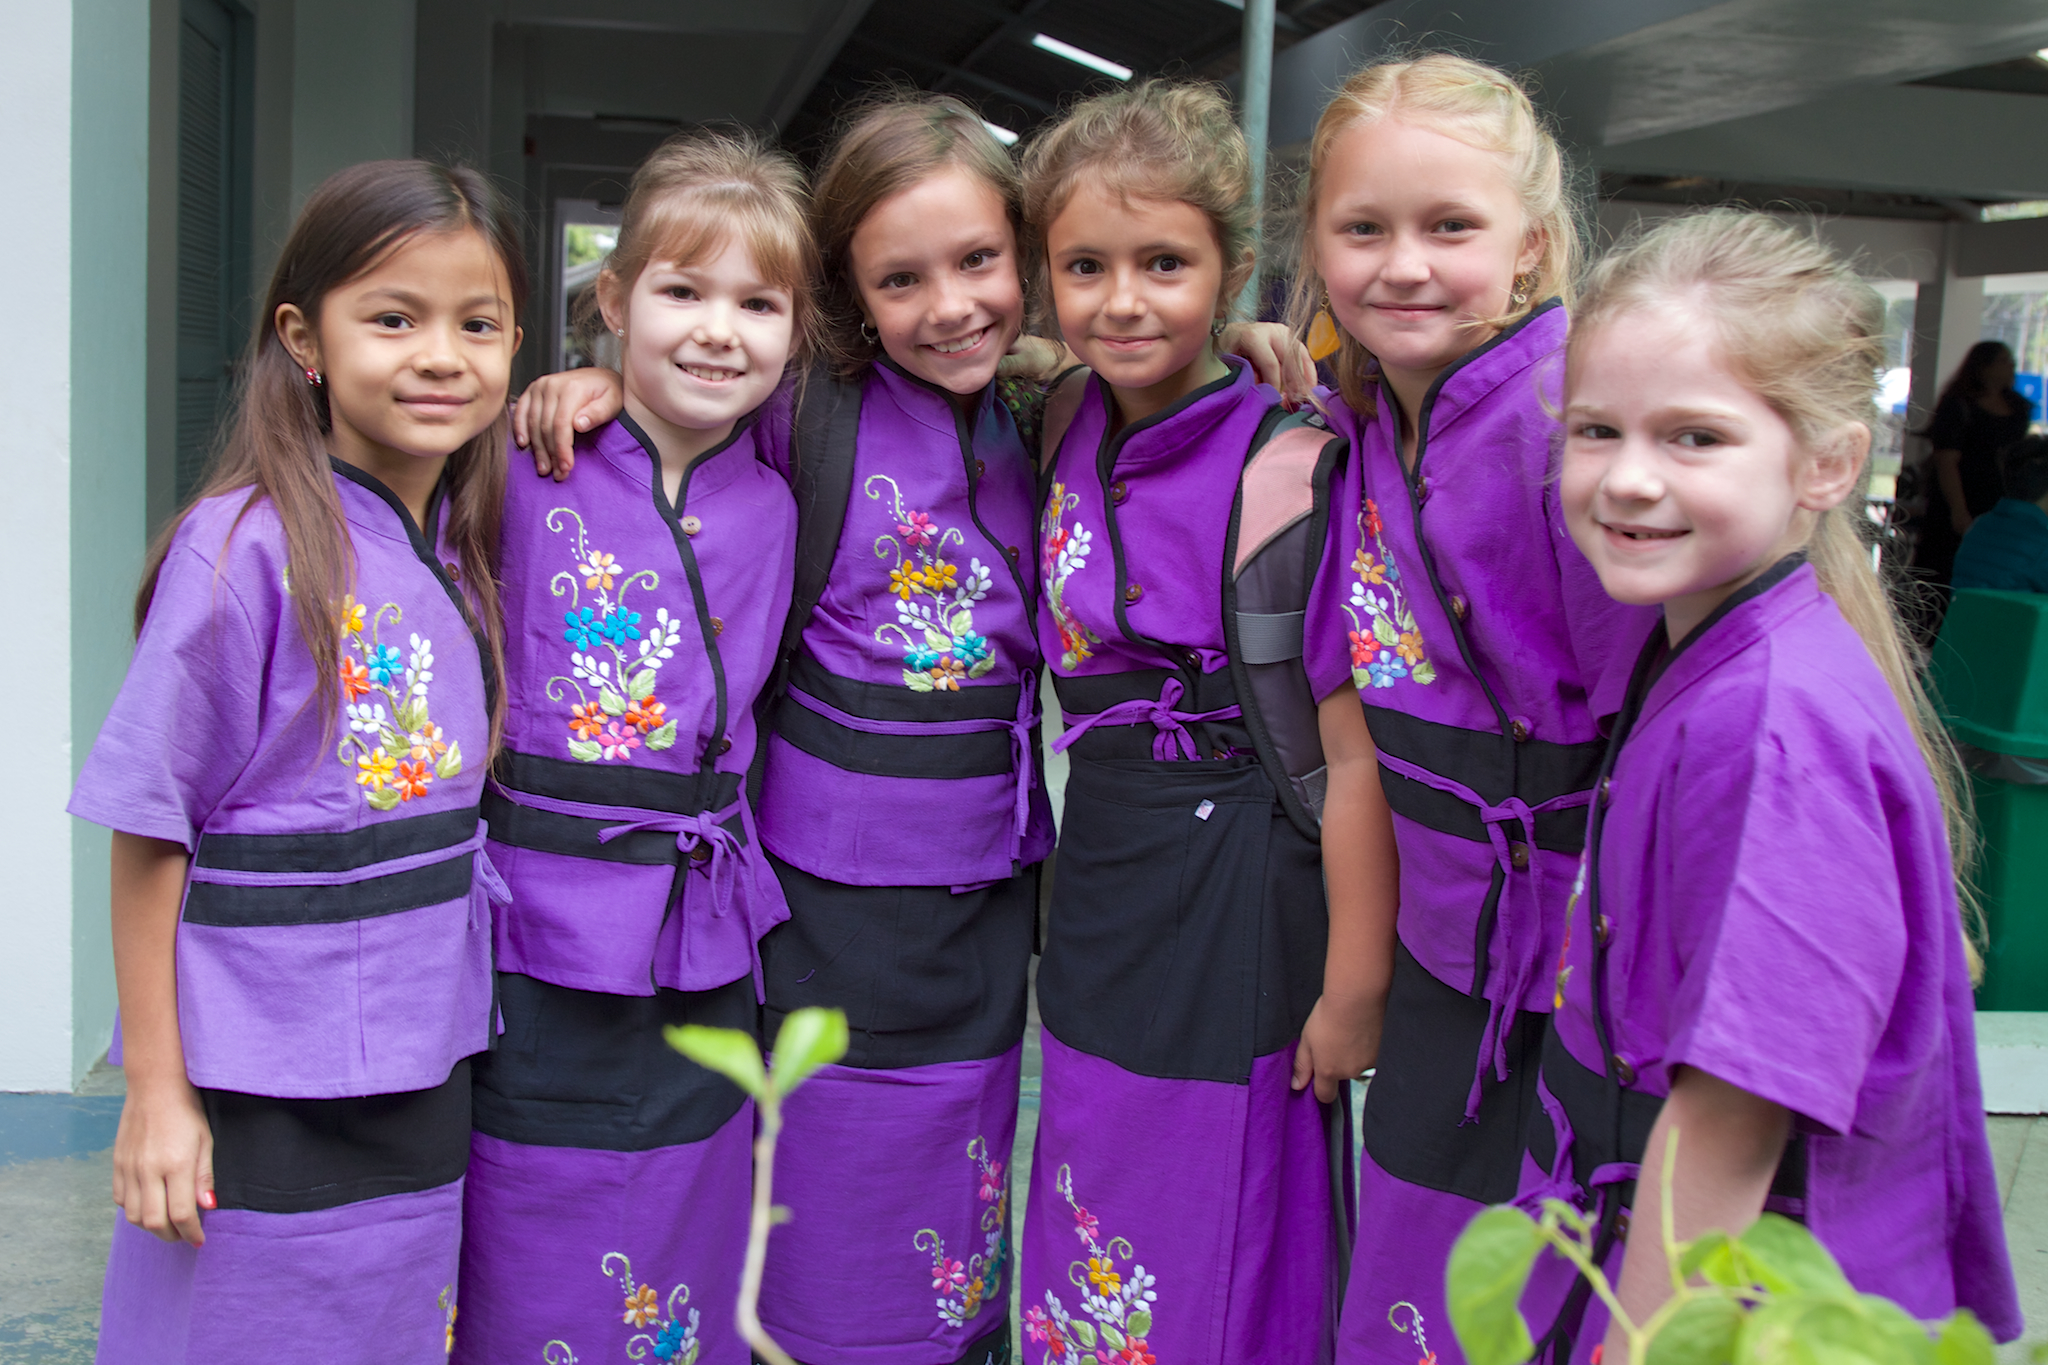
\includegraphics[width=\textwidth]{Preface.jpg}}

Though CMIS has grown significantly since the last self-study report in 2011 it has not lost sight of what it does best - ``Inspire educational excellence in a caring Christian community that respects and celebrates diversity.'' This has been accomplished through a combined effort to redefine the purpose of CMIS goals; improve student achievement and understand that it cannot be achieved without the whole community working together and supporting one another through appreciation, mutual respect, and understanding. This teamwork has brought about the realignment of standards, curriculum, and instructional practices that are research-based and anchored in 21st century skills. It has enabled the school divisions to participate in vertical and horizontal articulation that has resulted in stronger coherence. It has encouraged leadership to be a shared responsibility, where students, parents and staff have a collective voice and authentic opportunities to reflect on school practices, create meaningful plans for improvement, and seek effective ways to track progress. Most importantly, it has created a sense of cohesiveness and an understanding that self-improvement is a healthy process that is ongoing and essential in order to meet the diverse needs of CMIS students.




\tcbchapter{Student/Community Profile and Supporting Data and Findings}
\AddToShipoutPicture*{\BackgroundPic{chapter1.jpg}}
\tcbsection{CMIS Identifying Information}
\begin{description}
\item[Superindtendant]
Nel Capadona
\item[Year Established]
1954
\item[Last WASC Accreditation]June 2011
\item[Grades Accredited]PK-12
\item[Current Enrollment (May 1, 2016)] 498
\item[Enrollment At Last Accreditatixon (2010-2011)] 459
\item[Enrollment At Previous Accreditation (2004-2005)]401
\item[Current Number Of Teaching Staff (May 1, 2016)]73
\item[Number Of Teaching Staff At Last Accreditation (2010-2011)]57
\item[Number Of Teaching Staff At Previous Accreditation (2004-2005)]43
\end{description}


\subsection{CMIS: The School and the Community}

\minor{Introduction}

Chiang Mai International School (CMIS) is located just outside the old city of Chiang Mai, within the boundaries of the Superhighway. Chiang Mai is the largest significant city in Northern Thailand, and the former capital of the Lanna Kingdom.  

Founded in 1296 AD, Chiang Mai is a growing city with a unique balance of modern conveniences and historic culture.  It is located in the northern region of Thailand, approximately 720 km from Bangkok.  Chiang Mai covers an area of 20,170 sq. km. and supports a population of 1,682,164 (based on June 2015 data).  It is a predominantly agricultural area with a well-established manufacturing and service-based economy.  Because of the rich culture, pleasant climate, stable economy, and friendly, relaxed atmosphere, Chiang Mai attracts many expatriates.  Tourism is one of the major industries, attracting more than 2 million foreign visitors annually.  The area also supports local and international businesses, NGOs, and mission organizations, which employ foreign professionals.

Our school, the first international school in Thailand outside of Bangkok, has a long and rich history.  Our campus is a testament of this history.  From the beginning as an American Presbyterian missionary residence, to now as a 21st century school campus, the land on which CMIS sits has continually developed is a living and learning community with a strong sense of identity and a vision of educational excellence.  

\minor{Facilities}

Missionaries returning to work with the Church of Christ in Thailand (CCT) after World War II established a school for their children in Chiang Mai.  When CMIS was founded in 1954, the school was originally established in the McGilvary house (located on the First Church property along the Ping River).  Classes began with eight students on June 1, 1954.  In 1958, construction began on the present campus for the “Chiang Mai Children’s Center”.   Student numbers grew as more expatriate families seeking an English-language education for their children moved to Chiang Mai.

In 1984, representatives of the Thai Foreign Ministry and the CCT agreed that the formal establishment of an international school in Chiang Mai was a necessary step to achieving the school’s legal status.  Classes began in September 1985 for Kindergarten to Grade 8 under the new name “Chiang Mai International School” (CMIS).  High school grades were progressively added from 1992 to 1995.  

Our current campus is located in close proximity to private Thai schools, a hospital, a seminary and a university, all of which were founded by American Presbyterian missionaries and owned by the CCT.  The existing buildings on the CMIS campus, and their history of construction, are as follows: 
\begin{enumerate}
\item McKean House (Administration Building) (1906)
\item Pre-School Building (1958)
\item Library Building (1958)
\item Auditorium Building (1988)
\item High School Building (1990)
\item Elementary Building (1997)
\item Gymnasium Building (2007)
\end{enumerate}
Today CMIS is a dynamic international school with over 500 students, but is it is still small enough to retain a friendly and relaxed campus environment.  It also remains true to the traditions of its founders, serving missionary families and maintaining the heritage and values of the Christian faith at the heart of the school, while welcoming children of all faiths, cultures, and ethnic backgrounds from the growing international community in Chiang Mai.  

\minor{Development Plans}

Of the five main international schools in Chiang Mai, CMIS is the only one in close proximity to the center of the city.  With the growth potential promised by the ASEAN agreement, CMIS has looked toward expanding the current campus to meet the needs of the community while maintaining its characteristic close family atmosphere.  Short and long term campus development planning have been a huge focus for the past six years. There is now a long term plan that includes additional buildings and planned renovations to existing buildings.  The \href{https://docs.google.com/spreadsheets/d/12H8OtZlda_OBTVfUOYvEg0qghC6U9Xz93vGASmJF1hQ/edit#gid=0}{timeline for development} began in July 2014, and actual construction began in April 2016.  Construction of a new high school building, a covered court, a new library and cafeteria, and swimming pool are expected to be completed by December 2018.  Campus Development Timeline.  There are \href{https://docs.google.com/presentation/d/1o_AcPdYb1572Wbm7vk79ssg7RzkQykBGOqrKGVhTArw/edit#slide=id.ga51c5f54b_0_41}{ongoing renovation and enhancement projects} to maintain the \href{https://docs.google.com/presentation/d/1BSJvdHXlQ7o2US1hnvFOyPIcvA3WEPCRc9XYJAqlNt4/edit#slide=id.g540d23d42_034}{school grounds and existing facilities}.

\begin{figure}
\centering
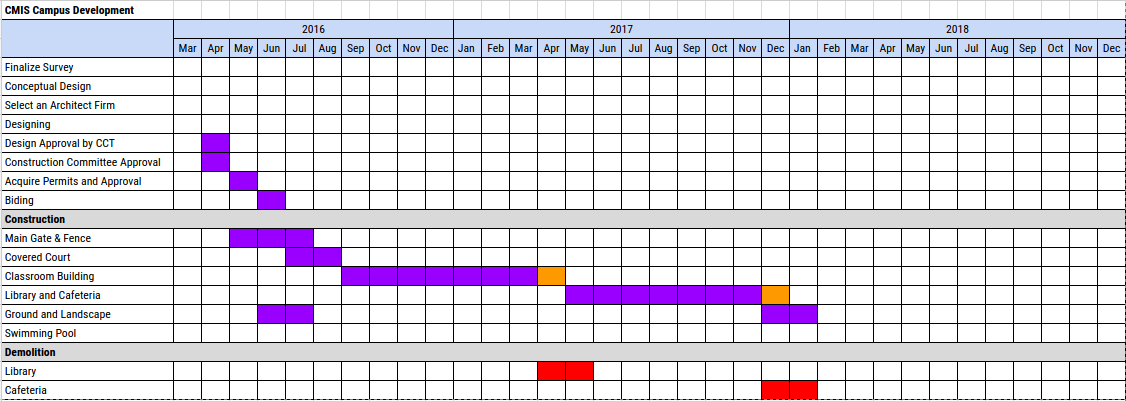
\includegraphics[angle=90, height=\textheight]{profile1}
\caption{Developement Timeline}
\end{figure}

\subsection{Vision and Mission}

\begin{figure}
\centering
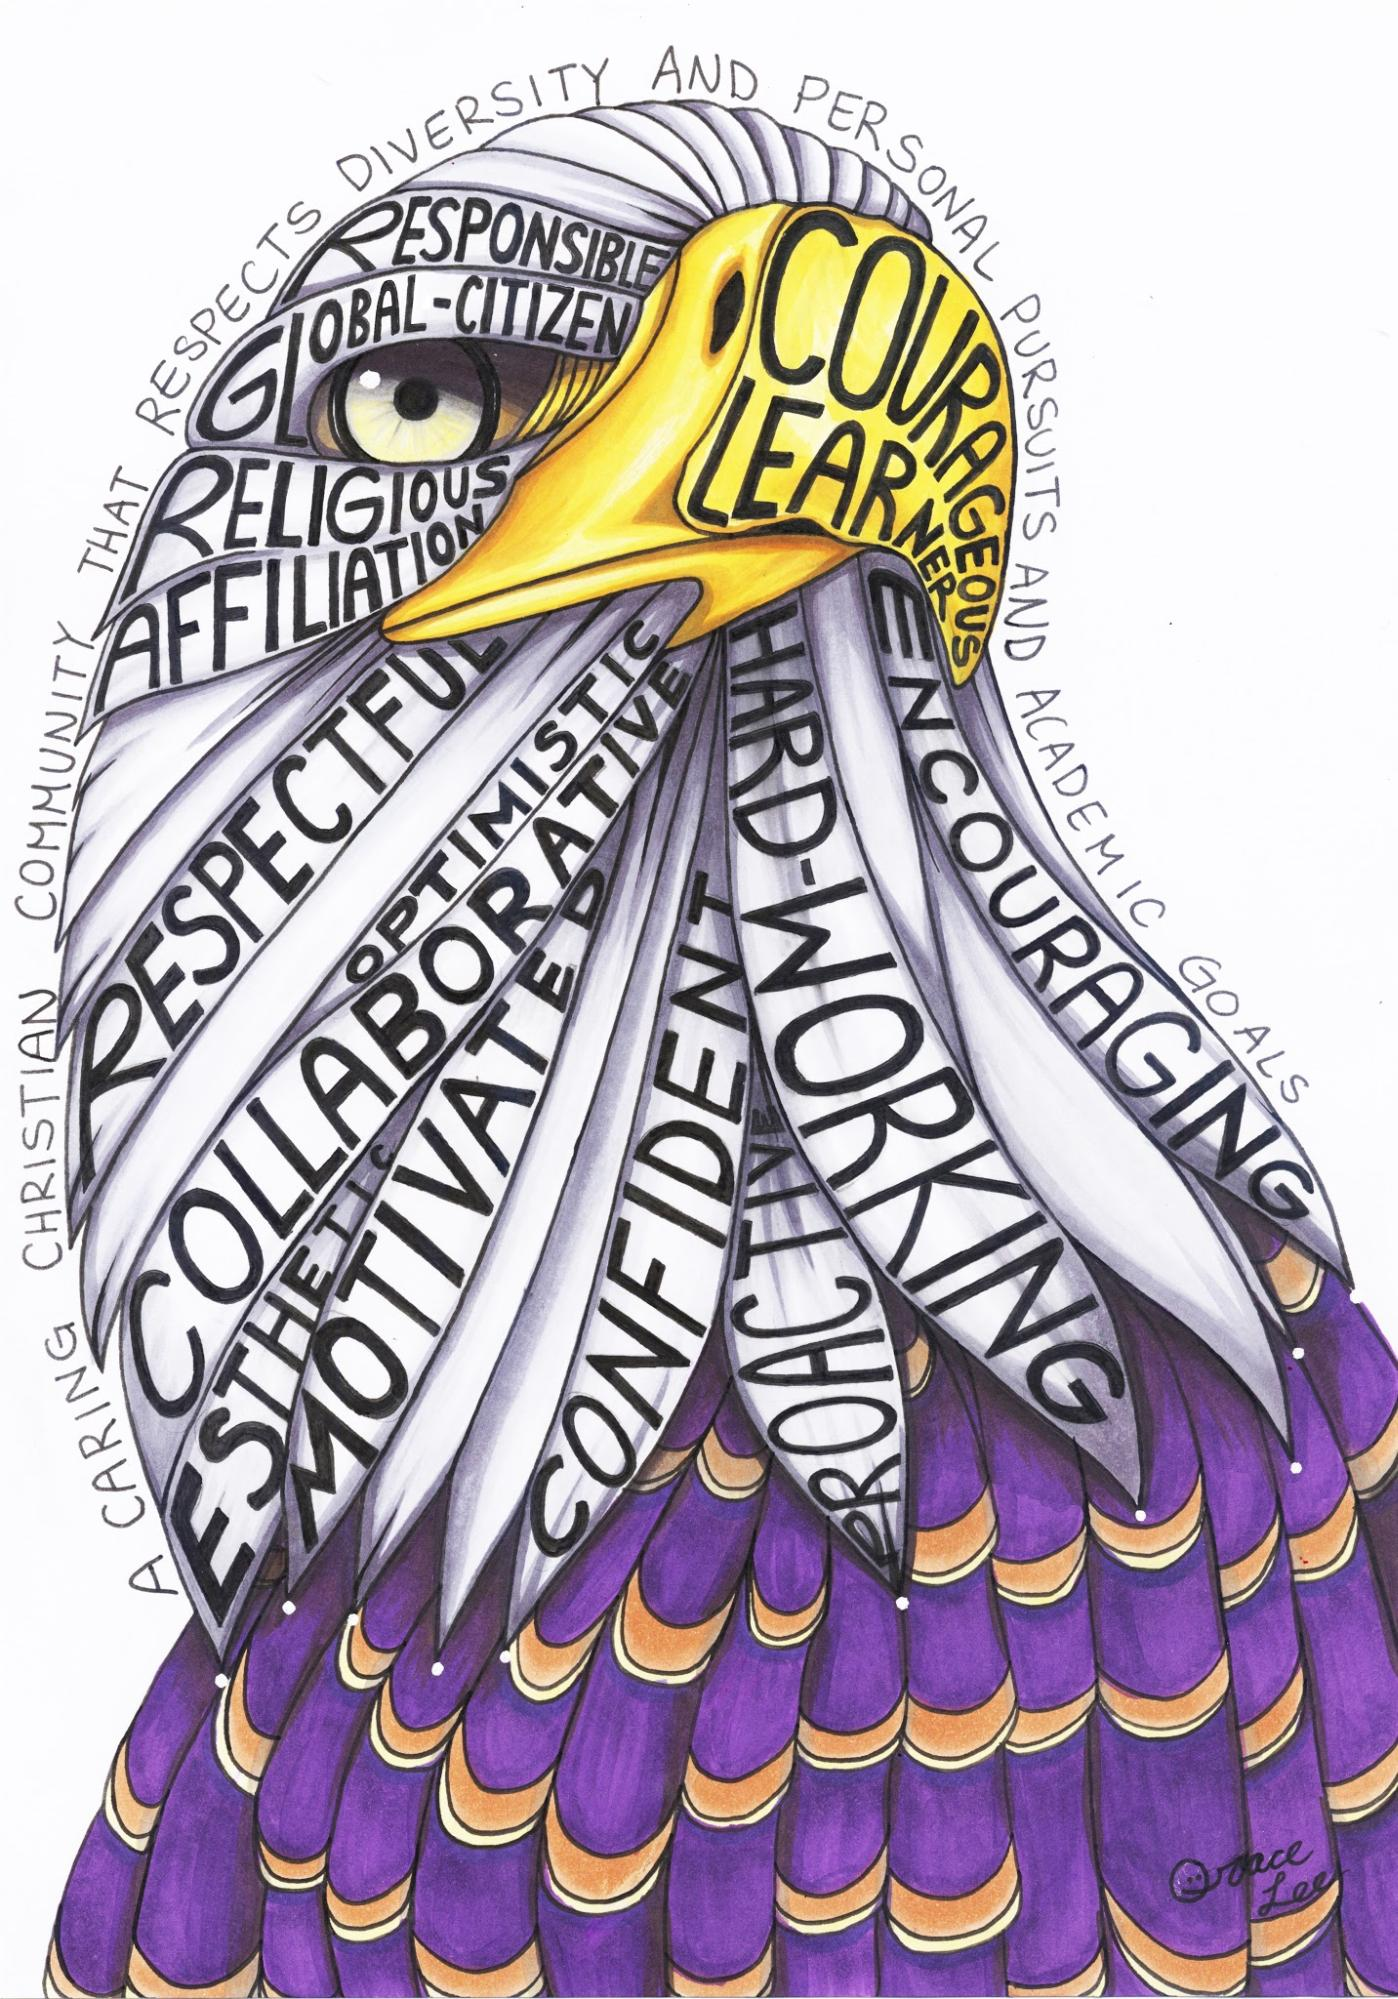
\includegraphics[width=\textwidth]{profile2}
\caption{CMIS Vision and Mission Logo}
\end{figure}

As a standards-based American curricular school, CMIS offers a challenging educational experience, rooted in Christian values, which helps develop students into global citizens; as reflected in the CMIS vision, mission statement, and learner outcomes.

\minor{CMIS Vision}
To provide educational excellence in a caring community, that respects and celebrates diversity.

\minor{CMIS Mission}
To develop learners who can pursue personal and academic goals, based on educational excellence and strong moral foundations. To equip students for lives of learning and positive contributions locally and globally.

\minor{Student Learner Outcomes}
Courageous learners who:
\begin{itemize}
\item Embody a work ethic that values learning and academic integrity
\item Pursue personal growth as adaptive, independent learners
\item Exhibit thinking that is open minded, creative, and takes risks
\item Utilize resources and technology to effectively support learning and work
\end{itemize}

Responsible global citizens who:
\begin{itemize}
\item Understand Christian virtues and positive student character
\item Demonstrate integrity through consistent respect for people of all faiths
\item Build cultural awareness and an appreciation for diversity
\item Serve as responsible, proactive members of the global community
\end{itemize}

\minor{Student Characteristics}

Excellence in academics and ability to form successful relationships in a multi-cultural Environment.

\minor{School Identity}
 
Developing academic excellence within a multicultural environment committed to Christian Values.

\minor{Religious Affiliation}

CMIS is a school with a clear Christian ethos.  Founded as part of the Church of Christ in Thailand, the national Protestant church, the operation of the school and all relationships within the school community are based upon Christian principles and beliefs with religious services and public prayers offered in the Christian tradition.  Within this spirit, CMIS encourages students to learn about God’s love and the Christian faith so they can make their own personal and intelligent response to it.  CMIS also warmly welcomes students and staff from differing religious backgrounds, cultures, and beliefs.


\minor{So what...}

The market for CMIS is dependent upon tourism and foreign business opportunities in Chiang Mai.  Changes in the economy, political environment, or immigration policies could potentially impact enrollment at CMIS.  Chiang Mai is a popular tourist destination and a pleasant place to live.  At present, the school is experiencing optimal enrollment and a favorable political and social climate.  Our caring community and adherence to Christian values makes us distinct among the other international schools in Chiang Mai.  Our school administrators remain sharply focused on our school mission and vision, while they implement decisions aimed at achieving our Student Learner Outcomes.  CMIS has implemented a development plan to modernize the facility and to accommodate the needs of our growing school community.  

\begin{figure}
\centering
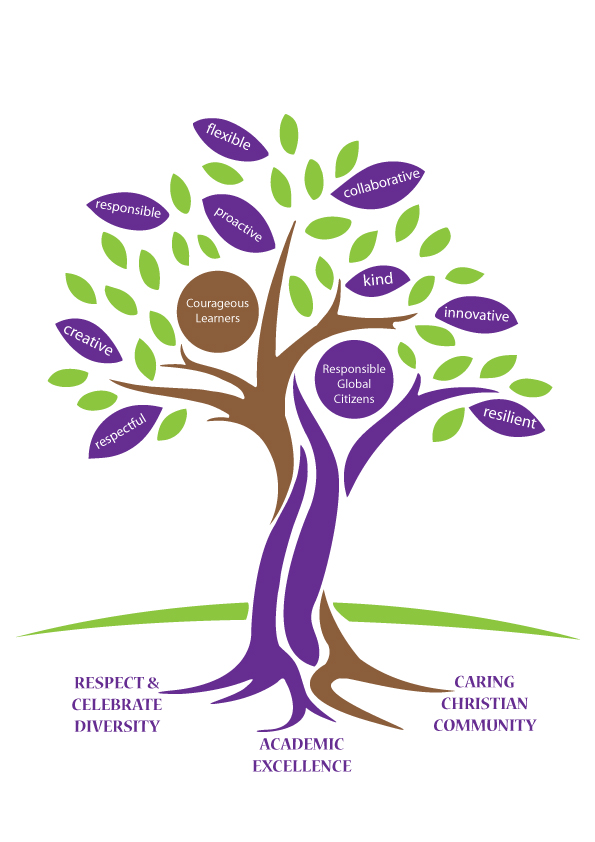
\includegraphics[width=\textwidth]{profile3}
\caption{Tree Logo}
\end{figure}


\tcbsection{Enrollment Patterns}

\minor{Enrollment 2012 - 2016}

Overall student enrollment has increased incrementally by 10 to 20 students per year over the past five academic years.  More than half of the increase came through filling existing vacancies in the Elementary School.  While the Elementary grew at an average rate of 6\% per year, total school enrollment increased by only 2\% per year.  Prior to 2012, Grade 6 was classified as Elementary, whereas from 2013 to present, Grade 6 is classified as Middle School.  Despite the categorical change, Middle School enrollment actually declined slightly throughout the reporting period.  In the 2016-2017 academic year, total school enrollment surpassed 500 for the first time in history.  

As with any international school, CMIS has a small percentage of students who withdraw each year. The resultant vacancies are offset by the enrollment of new students each year.  The balance of enrollment changes each year by accounting for the *previous year’s graduating seniors, adding new and returning students, and subtracting withdrawals.  That annual change is represented as follows:



\begin{table}[h]
\caption{CMIS Enrollment Changes}
\label{table:1}
\begin{tabu} to \textwidth {|X|X|X|X|X|}
\hline
 &
New/Returning*
 Students &
Graduation &
Withdrawals &
Net Increase \\
\hline
2012-2013 &
127 &
36 &
44 &
47 \\
\hline
2013-2014 &
106 &
39 &
59 &
8 \\
\hline
2014-2015 &
120 &
41 &
45 &
34 \\
\hline
2015-2016 &
113 &
38 &
65 &
10 \\
\hline
2016-2017 &
96 &
38 &
-- & 
pending \\
\hline
\end{tabu}
\end{table}

*Returning refers to students who previously attended CMIS, but who had withdrawn for at least one semester.  Continuing students are those who continue their enrollment at CMIS from one year to the next, without interruption.  

In the 2016-2017 academic year, the total number of Continuing vs. New and Returning* students by division is as follows:

\begin{table}[h]
\caption{Continuing vs. New and Returning}
\label{table:2}
\begin{tabu}{|X[2]|X|X|X|}
\hline
&
Continuing&
New/Returning&
Total\\
\hline
Elementary (PK - Gr. 5)&
168 (73\%)&
61 (27\%)&
229\\
\hline
Middle School (Gr. 6 - 8)&
88 (81\%)&
20 (19\%)&
108\\
\hline
High School (Gr. 9 - 12)&
151 (90\%)&
16 (10\%)&
167\\
\hline
TOTAL&
407 (80\%)&
97 (19\%)&
504\\
\hline
\end{tabu}
\end{table}

\minor{So what...}

CMIS replaces approximately 10\% to 20\% of its student body annually.  Sustained, incremental growth has brought us very close to the point of maximum capacity.  However, we have no particular data relating to the reasons people withdraw from CMIS; whether they are satisfied with their CMIS experience, or where they choose to study next.  Because this type of information is available through the Withdrawal Form and the issuing of a School Leaving Certificate, we should be able to obtain meaningful feedback from those who withdraw.  This presents us with an opportunity to survey our withdrawing families and reflect on any trends that might affect our overall enrollment status in the future. 
\tcbsection{Student Diversity}

\minor{Enrollment by Nationality 2015-16 / 2016-2017}

The CMIS student body represents a diverse international community, with students from over 30 different countries.  The largest single group are those who have dual passport status or parents from two different countries.  Many factors are taken into consideration when selecting our CMIS students.  Age, gender, and nationality are certainly among them.  However, academic potential, the ability to follow instructions, personal maturity, social skills, and overall potential to succeed are of greater importance.  Regardless of \href{https://docs.google.com/spreadsheets/d/15wjkZ9Yy__KpVuhKlawJuoMAAlCE6FMBsOJMKjXacYA/edit?ts=579eee90#gid=0}{nationality} or ethnic identity, all successful applicants must be qualified personally, socially, and academically.  

We give priority enrollment to qualified applicants from the Western world.  There are no restrictions placed on our dual citizens or those coming from Western countries, such as the United States, Canada, the UK, Australia, New Zealand, and English-speaking countries in Europe or Asia.  We do not make exceptions for our missionary or diplomatic communities, but we do reserve spaces for them and give them priority for acceptance, if qualified.  

In the 2016-2017 academic year, the percentage of American, Australian, Canadian, Dual, and United Kingdom students is as follows:

\begin{table}[h]
\caption{American, Australian/New Zealander, Canadian, UK, and Dual Citizenship}
\label{table:3}
\begin{tabu}{|X[2]|X|X|}
\hline
American & 117 & 23\% \\
\hline
Australian / New Zealander & 21  & 4\% \\
\hline
Canadian & 8 & 2\% \\
\hline
Dual & 118 & 23\% \\
\hline
United Kingdom & 26 & 5\% \\
\hline
\end{tabu}
\end{table}

Thai, Korean, Chinese, and Japanese applicants are considered on a space-available basis.  Our target goals for each of these populations compared to our current enrollment are as follows:

\begin{table}
\caption{Thai, Chinese, and Japanese Enrollment}
\label{table:4}
\begin{tabu}{|X[2]|X|X|X|}
\hline
Nationality &
Target &
Current Number &
Current Percentage \\
\hline
Thai &
25\% &
183 &
36\% \\
\hline
Korean &
20\% &
75 &
15\% \\
\hline
Chinese &
10\% &
24 &
5\% \\
\hline
Japanese &
10\% &
1 &
<1\% \\
\hline
\end{tabu} 
\end{table}

\begin{figure}
\centering
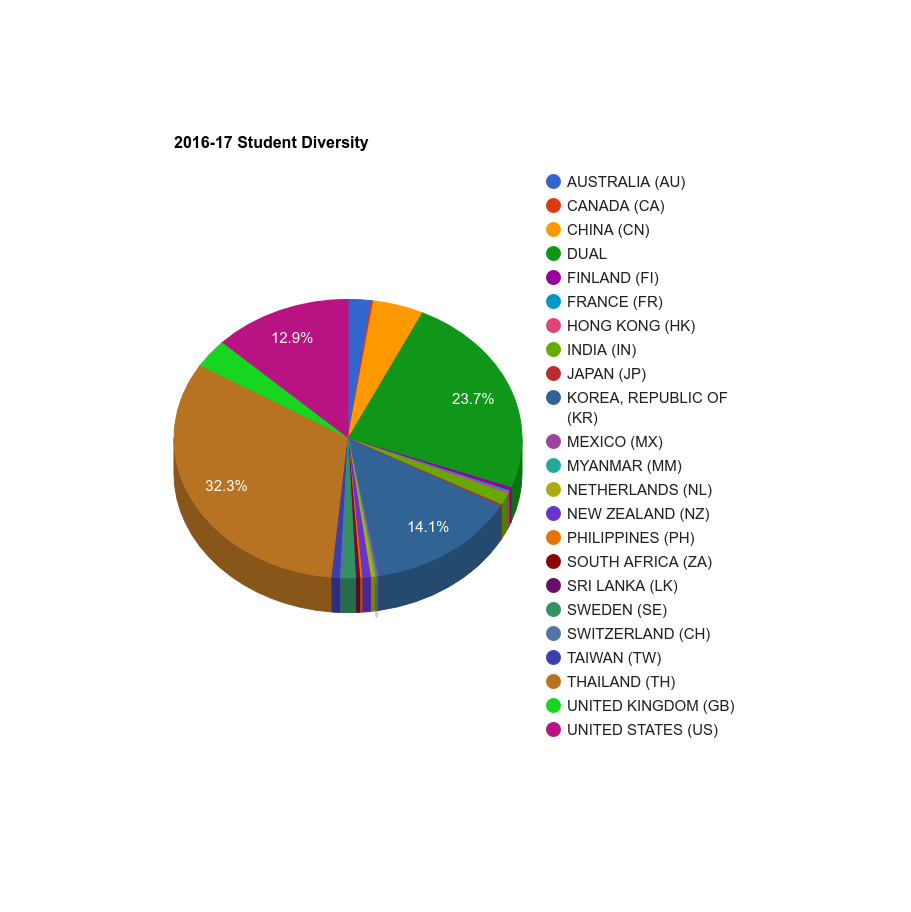
\includegraphics[width=\textwidth]{profile4}
\caption{Student Diversity 1016-2017}
\end{figure}

\begin{figure}
\centering
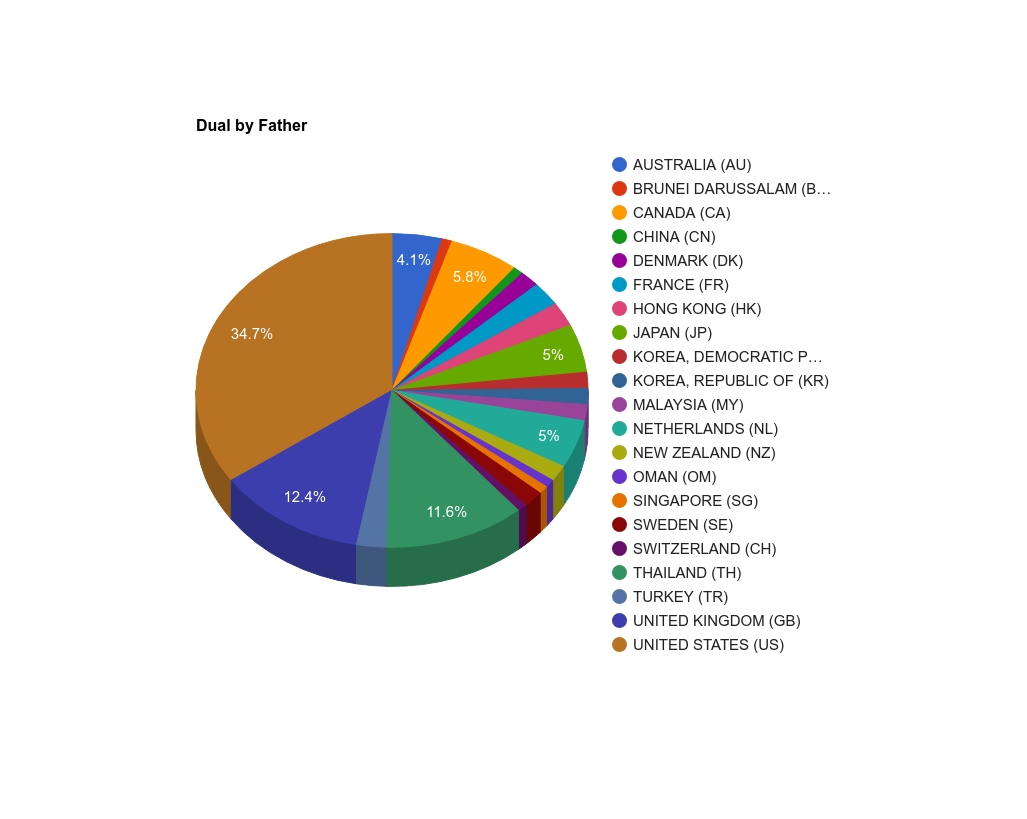
\includegraphics[width=\textwidth]{profile5}
\caption{Dual by Father}
\end{figure}

\begin{figure}
\centering
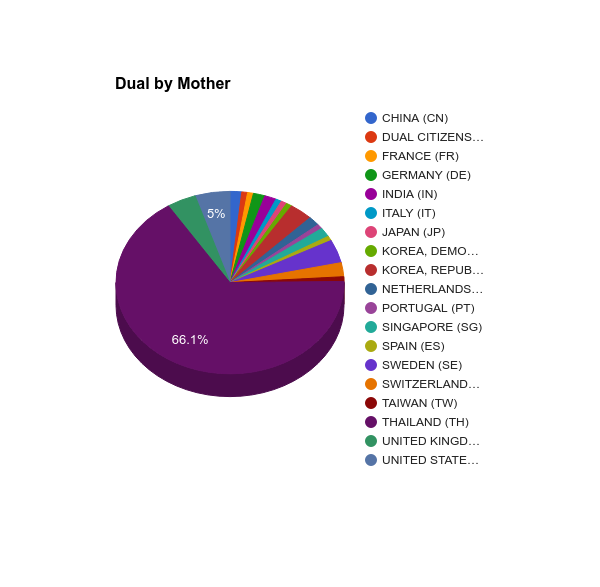
\includegraphics[width=\textwidth]{profile6}
\caption{Dual by Mother}
\end{figure}

\begin{figure}
\centering
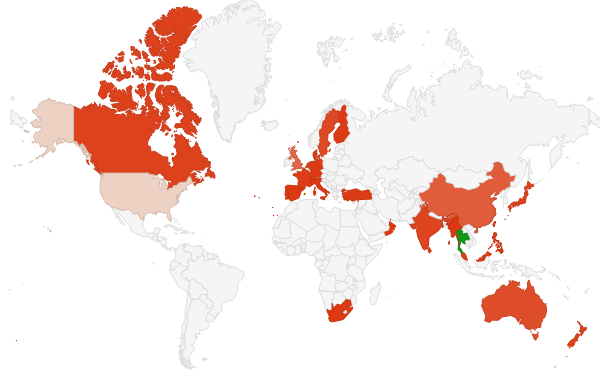
\includegraphics[width=\textwidth]{profile7}
\caption{Countries of Origin}
\end{figure}

\minor{Teacher/Student Ratios \& Gender Mix}

The ratio of Male (48\%) to Female (52\%) CMIS students remains relatively consistent throughout the student body, with some fluctuation in the Pre-School and Kindergarten grade levels.   With 77 staff in student contact positions (teachers, counselors, IAs) and 504 students, the Teacher / Student ratio is approximately 7:1.  

\begin{figure}
\centering
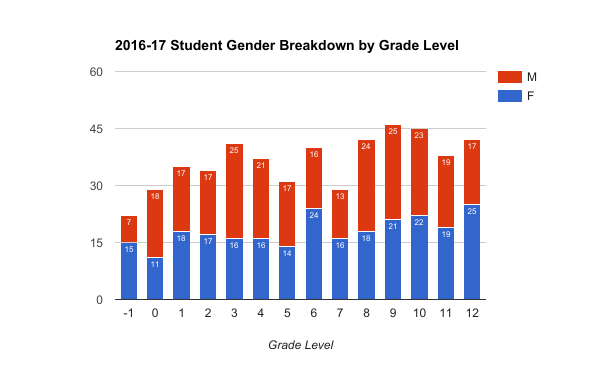
\includegraphics[width=\textwidth]{profile8}
\caption{Gender Breakdown by Grade Level (2016-2017)}
\end{figure}

\minor{So What...}

CMIS has experienced a period of sustained growth while maintaining ethnic and cultural diversity.  In order to maintain high academic standards in a diverse, English-speaking environment, admissions policies favoring Western applicants will remain in effect.  

\tcbsection{Criteria for Admission of Students}

\subsection{Application Process}

CMIS uses \href{https://cmis.openapply.com/}{Open Apply}, an online application system.  Applicants and enquirers are encouraged to register their interest, schedule an appointment for a meeting with the Admissions Director, and to complete their application electronically.  Applications for first semester enrollment are accepted from January through August.  Elementary and Middle School students may apply for enrollment at any time throughout the semester, provided that appropriate vacancies exist.  High School applications may be considered for enrollment up until the second week of the semester.  Applications received after the cut-off dates will be asked to delay their enrollment until the start of the following semester.  

Rare exceptions are made for High School applicants who are coming from abroad.  In those cases where families move to Thailand in mid-semester, qualified applicants may be accepted into High School in an auditing status.  These students are allowed to attend classes and fully participate in all classroom assignments and activities, although they will not receive credit for the semester course.  

\subsection{Standards for Entry}

CMIS strives to maintain a balanced, harmonious international environment where English is the language of inclusion.  We welcome applications from international students who:
\begin{enumerate}
\item Qualify academically (as determined by school records and standardized entrance assessment results) and
\item Meet the required English-language proficiency expectations for their grade level (as determined by CMIS guidelines).  
\end{enumerate}
CMIS strives to optimize class size to support individualized learning by setting a maximum number of students at the following levels:  

\begin{table}
\caption{Maximum Class Size by Level}
\label{table:5}
\begin{tabu}{|l|c|}
\hline
Level & Max \\
\hline
Pre-School &  12 \\
\hline
Kindergarten &  15 \\
\hline
Grade 1-2 &	18 \\
\hline
Grade 3-5 &	20 \\
\hline
Grade 6-12 &  25 \\
\hline
\end{tabu}
\end{table}

\minor{Language Proficiency}

Application to CMIS is competitive, and all students must have a minimum level of English language proficiency before they can be considered for enrollment.  The primary conditions for acceptance are academic eligibility, English-language proficiency, and exemplary behavior.  As part of the application process, applicants must submit copies of the current and previous year’s grade reports with teachers' comments, and any relevant standardized test results.  We can accept a limited number of academically qualified non-native English speakers, provided that their English-language proficiency falls within the CMIS guidelines for English Language learners. We can also accept a limited number for students with mild-to-moderate learning disabilities (as determined by previous school records, standardized testing, and Individualized Educational Plans), provided their disability falls within the CMIS guidelines for Learning Support (LS) and there is space available.

\minor{Age Requirements}

CMIS offers a Pre-School program for 4-year-old children who have reached their 4th birthday before the start of school in August.  The age / grade standard is set accordingly throughout elementary; age 5 for entry into Kindergarten, age 6 for grade 1, etc.  All applicants for Pre-School through Gr. 5 must have passed their required birthday by the start of school in August.  Students with birth dates after the start of school in August are classified according to their age on the first day of the academic year thus, any single CMIS grade level may have as much as 11 months of variability in the age of the students.  

For students who apply for entry to Middle School, applicants must have successfully completed the previous academic level and be within the appropriate age range for entry.  The \href{http://cmis.ac.th/admissions}{age/grade level} standard is adhered to as closely as possible.  Transferring into CMIS High School is dependent upon the number of credits on the student's transcript, compared to the CMIS \href{http://cmis.ac.th/programs/high_school}{graduation requirements}.

\minor{Entrance Assessments}

CMIS uses the Early Screening Inventory (ESI) for assessing Pre-School and Kindergarten applicants.  The test is scaled for children 3 years and 6 months old to 6 years 11 months.  Applicants for entry into Grades 1 through 11 are assessed with the WIDA (World-class Instructional Design and Assessment) to determine English-language proficiency.  The WIDA is divided into four grade level clusters:

\begin{itemize}
\item Grades 1 - 2
\item Grades 3 - 5
\item Grades 6 - 8
\item Grades 9 - 12
\end{itemize}


Each form of the WIDA assesses the four language domains of Listening, Speaking, Reading, and Writing.  

\minor{Priority Status}

Although we expect to have annual vacancies at each grade level, we reserve spaces for qualified, priority applicants.  Our Priority Categories are as follows:  
\begin{itemize}
\item Christian Missionary families,
\item Diplomatic / Consular families,
\item NGO / Non-profit organization families,
\item Siblings of current CMIS students,
\item Former CMIS families who are returning from abroad
\item CMIS Staff children, and
\item Fluent English speakers coming from comparable international schools
\end{itemize}

All other applicants are considered on a space-available basis.

In brief, applicants are required to:

\begin{itemize}
\item qualify academically (above average grades in a comparable academic system)
\item demonstrate the English-language proficiency expectations for their grade level
\item fit into a CMIS priority category or add value to our CMIS community
\item succeed academically without ESL or LS, or fit our criteria to qualify for those support programs
\item meet behavioral, emotional and social expectations of the CMIS student body
\end{itemize}

\subsection{Admissions Committee Review Process}

The CMIS Admissions Committee is responsible for making all decisions regarding student applications. The Committee consists of the Admissions Director, School Superintendent, Dean of Students, Elementary Principal, Elementary Counselor, Middle School Counselor, and High School Counselor.    Learning Support Specialists serve as adjunct members of the Committee, and may be asked to comment, provide additional assessment, or recommend further testing.  

In their assessment of an application, the Committee takes the following information into account:

\begin{itemize}
\item applicant's profile
\item previous academic background
\item performance on CMIS entrance assessment
\item English-language ability
\item availability of space at the recommended grade level/support program
\end{itemize}

The Committee determines the applicants’ qualifications for each criteria by:

\begin{itemize}
\item reviewing academic records (minimum of 2 years, as appropriate) and standardized test results
\item conducting entrance assessments
\item reviewing psychologists' assessments or other supporting documentation
\item meetings with the applicant and family
\item reviewing letters of recommendation
\end{itemize}

CMIS uses Open Apply, an online application system.  Applicants and enquirers are encouraged to register their interest, schedule an appointment for a meeting with the Admissions Director, and to complete their application electronically.  

Newly admitted students’ families are given a New Family Survey to help identify areas we need to focus; both in terms of the student application process and advertising. We use this data to refine how we reach our target audience and provide a better experience for our new families.

\tcbsection{School Finance}

CMIS is a privately owned, not-for-profit school.  The \href{https://docs.google.com/document/d/1j2Z1tLgRgfX9CH3dzoYtU_GOhPOVWKPl6iFlvWqd6wM/edit?usp=sharing}{tuition and fee schedule}, as well as the annual operating budget, must be approved annually by the Administrative Advisory Board (AAB). 

\minor{Tuition Rate Categories}

In the 2011-2012 academic year, CMIS instituted a Standard Tuition rate.  All new students from that time onward are classified in the Standard rate category unless the student’s family is eligible for one of the reduced (Discount or Self-Funded Missionary) rate categories.  Those existing CMIS families at that time were automatically grandfathered into the Discount rate category.  This Discount rate also applies to those new expat families who work with NGO’s or Non-profit organizations.  Thus, tuition and fees vary based on each student’s tuition category.  Staff children receive free education as a benefit of their parents’ employment, so Staff children are not required to pay tuition and fees.  

The number of students in each rate category over the past five years is as follows:
\begin{table}[h]
\caption{Tuition Rate Category}
\label{table:6}
\begin{tabu}{|X|X|X|X|X|X|}
\hline
Year &
Standard &
Discount &
Self-Funded &
Staff &
TOTAL \\
\hline
2011-2012 &
45 (10\%) &
230 (52\%) &
128 (29\%) &
38 (9\%) &
441* \\
\hline
2012-2013 &
85 (19\%) &
194 (43\%) &
141 (31\%) &
28 (6\%) &
448* \\
\hline
2013-2014 &
118 (25\%)	 &
174 (37\%) &
136 (29\%) &
43 (9\%) &
471 \\
\hline
2014-2015 &
161 (33\%) &
145 (30\%) &
133 (27\%) &
47 (10\%) &
486 \\
\hline
2015-2016 &
211 (42\%) &
118 (24\%) &
124 (25\%) &
43 (9\%) &
498 \\
\hline
2016-2017 &
250 (49\%) &
92 (18\%) &
118 (23\%) &
47 (9\%) &
507 \\
\hline
\end{tabu}
\end{table}

* Excludes Pre-School.  

\begin{figure}
\centering
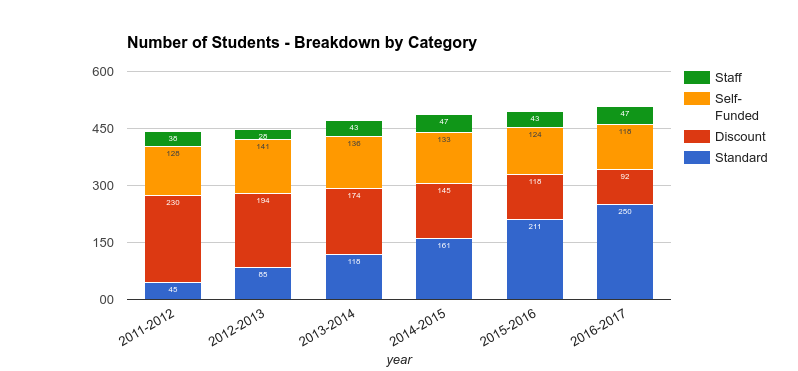
\includegraphics[width=\textwidth]{profile9}
\caption{Number of Students by Category}
\end{figure}

Over time, the number and percentage of students in the Standard rate category has increased, while the number and percentage in the Discount rate and Self-Funded Missionary categories has incrementally decreased.  Consequently, the annual income has increased accordingly.  (The number of staff children receiving free tuition has fluctuated with natural changes in our teaching and administrative staff. )  
 
\minor{Income and Expenses}

The graphs below represent the 2016-2017 budget and show anticipated income and categorical projected expenses.  

\begin{figure}
\centering
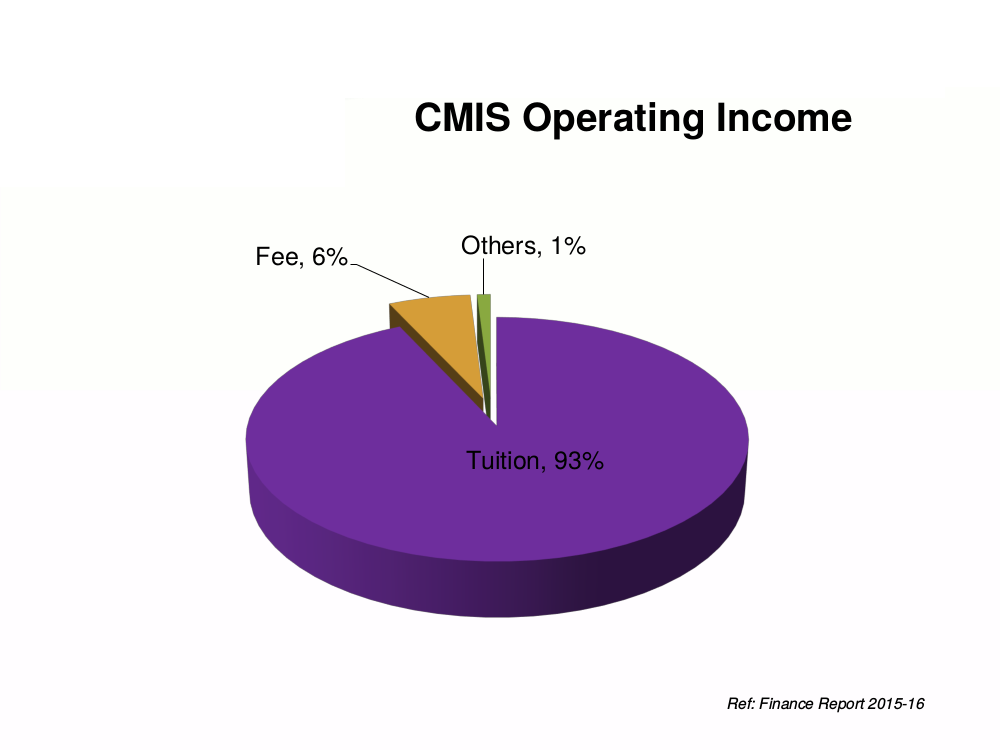
\includegraphics[width=\textwidth]{profile10}
\caption{CMIS Operating Income}
\end{figure}
\begin{figure}
\centering
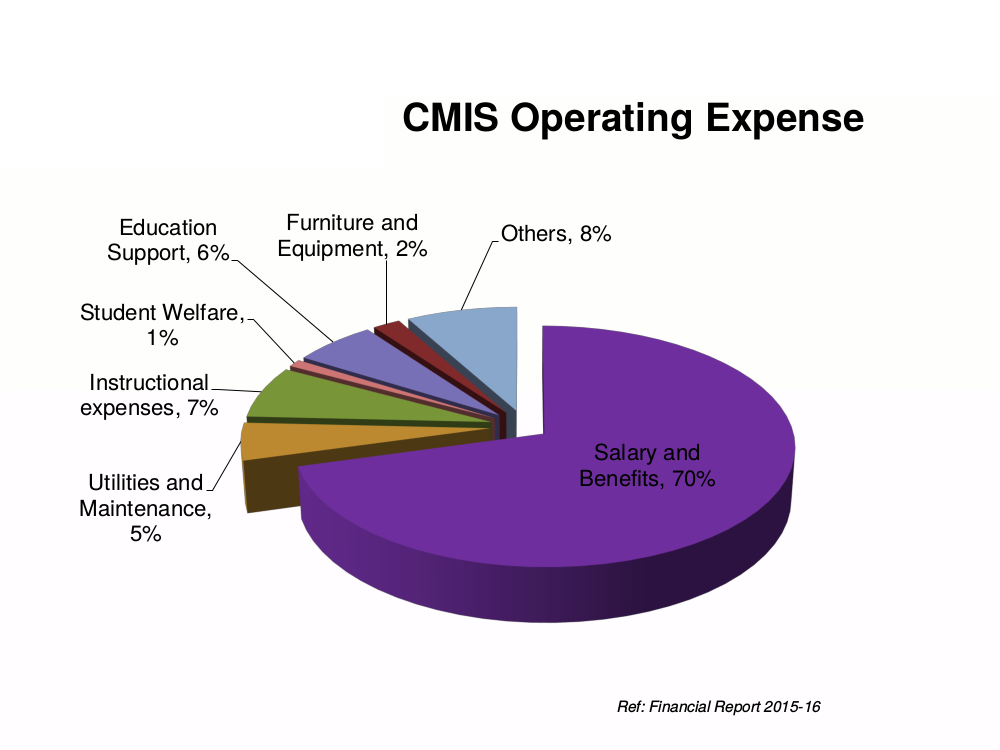
\includegraphics[width=\textwidth]{profile11}
\caption{CMIS Operating Expense}
\end{figure}

\tcbsection{Faculty and Staff}

\subsection{Administrative Leadership}

CMIS is licensed by the Ministry of Foreign Affairs, owned by the Church of Christ in Thailand (CCT), a national Protestant organization, and operated through a nine-member Board of Directors.  The day-to-day activities of the school are run by a School Management Team (SMT) composed of a Director (Thai), a Superintendent (non-Thai), two Principals (Pre-K - 8 \& High School; non-Thai), a School Manager (Thai), and an Assistant School Manager (Thai). 

\begin{itemize}
\item Director:  Manoonvatana Sirisujin         		director@cmis.ac.th
\item Superintendent:  Ronelda (Nel) Capadona	superintendent@cmis.ac.th
\item ES/MS Principal:  Tyler Stinchcomb	     	elementary@cmis.ac.th
\item HS Principal:  Aaron Willette		   	hsprincipal@cmis.ac.th	
\item Manager:  Patcharin (Nang) Jingkaojai		manager@cmis.ac.th
\item Asst. Manager:  Peay Tananone			assistant\_manager@cmis.ac.th
\end{itemize}

\minor{School Executive Team}

The school executive team (SET) is made up of the director, manager, and superintendent. The SET is responsible for implementing the school vision and mission, and serving as a bridge between the Administrative Advisory Board (AAB) and the school.  They meet weekly to make high level decisions affecting school policies and procedures.  SET members also serve in un-elected positions on the School Board.  

The current school executive team members are:

\begin{itemize}
\item Manoonvatana Sirisujin (CMIS Director) 
\item Patcharin Jingkaojai (CMIS Manager) 
\item Ronelda Capadona (CMIS Superintendent) 
\end{itemize}

\minor{School Management Team}

The school management team (SMT) exists to further implement SET decisions.  The SMT is responsible for the day-to-day, administrative, operation of the school.  The SMT would be involved with issues affecting the school facility, curriculum, and student body. The SMT consists of the SET plus the Assistant Manager, the Elementary/MS Principal, and the High School Principal. 

The current school management team members are:

\begin{itemize}
\item Manoonvatana Sirisujin (CMIS Director) 
\item Patcharin Jingkaojai (CMIS Manager) 
\item Ronelda Capadona (CMIS Superintendent)
\item Tyler Stinchcomb (CMIS Elementary / Middle School Principal)
\item Aaron Willette (CMIS High School Principal)
\item Peay Tananone (Assistant Manager)
\end{itemize}

\minor{Administrative Advisory Board (AAB)}

CMIS is owned by the Foundation of the Church of Christ in Thailand (CCT), and is governed through a Board of Directors comprised of a Board Chair (appointed by CCT); the CMIS School Executive Team; an elected representative from the PTG; an elected representative from the teaching staff; and additional members appointed by the CCT.

The current school board members are: 

\begin{itemize}
\item Rev. Dr. Esther Wakeman (Chair)
\item Rev. Dr. Sharon Bryant (Secretary)
\item Dr. David Filbeck
\item Kathryn McDaniel
\item Manoonvatana Sirisujin (CMIS Director) 
\item Patcharin Jingkaojai (CMIS Manager) 
\item Ronelda Capadona (CMIS Superintendent) 
\item Pascal van Geest (PTG Representative)
\item Brad Schmock (Teacher Representative)
\end{itemize}


The Roles and Responsibilities of the Board (as listed on page 9 of the Student Planner) are included below:

Role of the Board of Directors
\begin{description}
\item [Strategic Planning and Thinking] The Board of Directors develops and maintains the strategic plan for the school, guiding decisions on the organizational level in terms of program, facilities, etc., while keeping in mind the overall vision and mission of the school.
\item [Setting Policy] The Board of Directors oversees the development of policy for school operations. Hiring, evaluating and supporting of the School Leadership Team (Director, Manager and Superintendent) is a key responsibility of the Board. The Board of Directors is not involved in the day-to-day operations of the school, but supports the school leadership in developing the necessary skills and resources to run the school effectively.
\item [Financial Stability] The Board of Directors is responsible for the financial stability of the school and thus sets tuition rates and approves annual budgets.
\item [How Does the Board Govern?] The Board of Directors generally meets once a month from July through June.  Board members should be committed to attending every board meeting, but the board is also understanding of other constraints of members’ time.
\end{description}

\subsection{Professional Staff}

There are currently 65 full-time, \href{http://cmis.ac.th/about/faculty}{professional foreign staff} at CMIS, compared to 57 at the time of our last accreditation (2010-2011).  Increases have come mainly through adding institutional support positions, including Instructional Assistants (IAs) in the lower elementary classrooms, an Elementary Guidance Counselor, an Elementary Learning Support Specialist, and a High School Principal.  An Assistant Manager position was also created to facilitate the implementation of the Building and Facility development plans.  

\begin{table}[h]
\caption{Total Staff by Department}
\label{table:7}
\begin{tabu}{|X|c|c|}
\hline
&
PK-12 \\
\hline
Admin assistants &
2 \\
\hline
Facilities \& Maintenance &
21 \\
\hline
General &
1 \\
\hline
health/nurse &
2 \\
\hline
Office Staff &
20 \\
\hline
Thai Admin &
3 \\
\hline
Grand Total &
49 \\
\hline
\end{tabu}
\end{table}


\begin{table}[h]
\caption{Total Staff by Department}
\label{table:9}
\begin{tabu}{|X|X|X|X|X|X|X|X|}
\hline
	 &
ES/MS &
HS &
MS &
MS/HS &
PK-12 &
PK-5 &
Grand Total \\
\hline
Counselors &
&
1 &
1 &
1 &
&
1 &
4 \\
\hline
Foreign Admin &
1 &
1 &
&
&
4 &
&
6 \\
\hline
IA (Thai) &
&
1 &
&
&
&
7 &
8 \\
\hline
learning support & 
&
&
&
&
4 &
&
4 \\
\hline
teachers &
&
15 &
4 &
11 &
&
21 &
51 \\
\hline
Thai teachers &
&
3 &
2 &
1 &
1 &
3 &
10 \\ 
\hline
Grand Total &
1 &
21 &
7 &
13 &
9 &
32 &
83\\
\hline
\end{tabu}
\end{table}

\minor{Staff Diversity}

Our teachers and administrators are well-qualified professionals from 15 different countries, including:  the U.S. (31), Thailand (25), Canada (8), the U.K. (6), the Philippines (2), Myanmar (2), Australia (1), Switzerland (1), the People’s Republic of China (1), France (1), India (1), Mexico (1), the Netherlands (1), Norway (1), and Sweden (1).  More than one-third of our teachers and administrators hold advanced degrees.

\begin{figure}
\centering
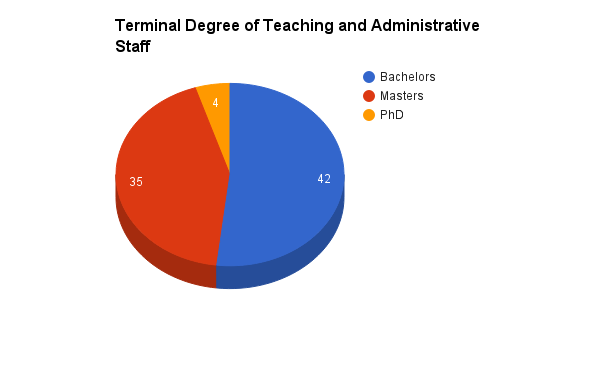
\includegraphics[width=\textwidth]{profile12}
\caption{Terminal Degrees of Teaching and Administrative Staff}
\end{figure}

\begin{figure}
\centering
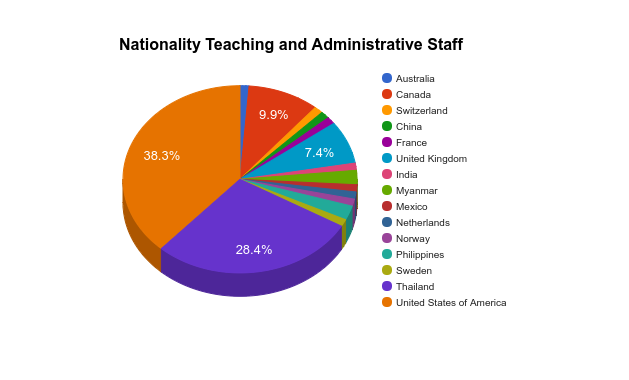
\includegraphics[width=\textwidth]{profile13}
\caption{Nationality of Teaching and Administrative Staff}
\end{figure}

\begin{figure}
\centering
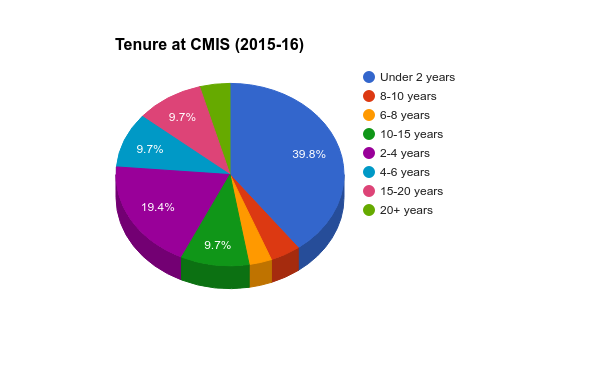
\includegraphics[width=\textwidth]{profile14}
\caption{Tenure at CMIS (2015-2016)}
\end{figure}

\tcbsection{Staff Professional Development}

CMIS is committed to providing and supporting professional development opportunities for its full-time teachers to improve teaching and student learning. This commitment is grounded in the belief that professional development is a continuous process, one which may be individualized depending on the skills and needs of the teacher; for the purpose of benefiting the teacher, CMIS and its students.  Any professional development opportunity should be related to schoolwide, student learning focus. 

The quality of our Teachers has been identified as the main factor in attracting new students to CMIS.  Recognizing that, CMIS provides teachers and staff with high quality professional development opportunities, both internally and externally.  

CMIS promotes the continued professional development of its teachers in the following ways:

\begin{itemize}
\item On-site scheduled professional development (scheduled during staff meetings and early release days).
\item CMCIS  PD Day - a joint day of collaboration and professional development for schools in the CMCIS, Chiang Mai Circle of International Schools
\item Advanced Placement (AP) Training.  
\item Chiang Mai based Conferences and Seminars. 
\item Online courses and seminars.  
\item Conferences and seminars held in Thailand. 
\item EARCOS Conference.
\item  Out-of-country conferences and seminars. 
\item Sharing the Experience.  Upon the staff member’s return to school, he or she is expected to share with the school what was learned.  Staff members are also required to file a written assessment of the program through the Professional Development Assessment Form that will be made available for other staff to review.
\end{itemize}


\minor{Designated Funding}

In addition to school/department wide professional development, the school provides funding in the amount of 10,000 Baht for each school year (starting in the 2013-14 school year), for each full-time teacher to engage in professional development (PD) opportunities.  PD funds can be accrued up to 5 years. Any (projected) unspent amount will be returned to the general PD fund at the end of the 5-year period or earlier if the teacher leaves CMIS employment. Since 2014, the school has utilized over 1,370,000 baht from the professional development budget.

The professional development (PD) budget may be used toward recertification, workshops, conferences, professional memberships, or position-specific training.  Travel, per diem, accommodation, registration, tuition, and required materials are also eligible for reimbursement, based on established guidelines.  Transportation budgets are limited, and staff are encouraged to look for PD opportunities within the region.  

All professional development funding and leave must be approved by the divisional principal, superintendent, or director.  All applications for professional development are considered carefully based on the following:

\begin{itemize}
\item Location of the event with priority set in the order of Chiang Mai, Thailand, SE Asia, outside of SE Asia, as well as if the course or seminar is offered online.
\item Relevance to the school wide, student learning focus.
\item Benefit to CMIS.
\item Length of time away from school.
\item Budget availability (early application is best for this).
\item Timing of request, advanced notice is preferred.
\item Staff member’s seniority or stated plans to stay at CMIS.
\end{itemize}

\begin{figure}
\centering
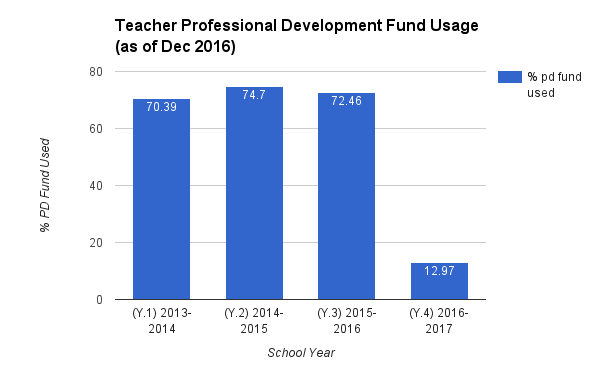
\includegraphics[width=\textwidth]{profile15}
\caption{Teacher Professional Development Fund Usage (as of December 2016)}
\end{figure}

CMIS Teachers and administrators are hired on two-year contracts.  More than half of our foreign staff (59\%) have been in their current positions for four years or less, while 25\% have been here for 10 or more years. 

\tcbsection{Teacher/Administration Communication Team (TACT)}

CMIS employees should have a safe and positive working environment. We understand that when working as a team, misunderstandings or miscommunication may occur.  In an effort to alleviate this, CMIS created the Teacher Administration Communication Team (\href{https://docs.google.com/a/cmis.ac.th/document/d/14nhwcw8xo3i-23Q-WUxo6KJ_c8yFKu-jTdCctt4MFcs/edit?usp=sharing}{TACT}) in 2013. The team is comprised of teacher reps from each division and the school executive team. The team meets regularly to review and address current staff concerns and a \href{https://docs.google.com/a/cmis.ac.th/document/d/1KLB4c5_LkxXzq4vP2EuNhBVPp2q_FT9qy1cBBwaS5JM/edit?usp=sharing}{summary} of the solutions and suggestions are e-mailed out to all staff.

The purpose of the \href{https://docs.google.com/document/d/12ZwL4geAPTDcm-SI6U1fRpXEKxKZ-61q54upcikt6lc/edit}{TACT} is to foster and create the best learning environment possible for our students by improving the overall happiness and satisfaction of faculty. We believe that when we invest in the well being of people, we invest in the long-term success and viability of CMIS.

To this end, the role of TACT is to provide a way for faculty to raise issues, concerns, and questions to the CMIS Executive Team (Director, Superintendent, Business Manager).  CMIS prefers that individuals address issues, concerns, and questions directly to their building administration (the principals of the elementary, middle, and high schools).  There are times, however, when individuals may not feel comfortable in speaking with building administration or leadership; thus TACT can forward these issues on their behalf.

\begin{itemize}
\item we believe in positive intentions, and that all stakeholders share the same vision of the best possible learning environment for CMIS students
\item we believe in openness and transparency in decision making and communications
\item we believe in equity - the fair and impartial treatment of others
\item we believe that praise and recognition produces far better results than criticism or punishment
\item we believe in social sustainability and social responsibility
\end{itemize}

\tcbsection{Parent Teacher Group (PTG)}

Teachers, administrators and parents or guardians of CMIS students are all automatically members of the Parent Teacher Group (PTG). The PTG is the "voice" at CMIS, as it provides a forum for sharing ideas and concerns about the school, and creates opportunities for parents and staff to establish friendships and networks within the CMIS community. The primary objectives of the PTG are:

\begin{itemize}
\item To promote communication between CMIS parents, teachers and administrative staff.
\item To promote and actively support CMIS educational programs, sports, activities and events.
\end{itemize}
 
The PTG achieves this through volunteer work and fundraising.  The PTG welcomes and encourages all parents and teachers to take an active role in the school by attending monthly meetings, and by volunteering time, resources and abilities to make CMIS the best place that it can be for our students.

The PTG serves as a conduit of communication between teachers, administrators, parents, and members of the school community.  

\tcbsection{Non-Academic Activities}

\subsection{Beyond the Classroom}

CMIS offers opportunities for student growth and personal development through Student Life Beyond the Classroom programs and activities.  

\minor{What is Student Life?}

“Student Life” is a common division, department, or office found on university and college campuses across the United States of America.  These divisions can be designed to meet a broad range of student needs/concerns, but they all have the basic goal of helping students get the most out of their experiences at school by supporting student opportunities away from the classroom.  At CMIS, student life is defined as the beyond the classroom opportunities which align with the CMIS Mission Statement and allow for personal, social, spiritual, intellectual, artistic, and physical growth.

\minor{Faith and Service}

CMIS encourages faith and service outside the classroom by allowing students to pursue their unique interests both on and off campus. The school invites students to initiate their own faith-based groups, and it encourages students to use school facilities to hold meetings and events.  In 2015, CMIS created a position of  a Student Spiritual Advisor.  The advisor is a faithful role model and spiritual guide for not only our Christian students, but all students. The advisor is there to listen to the students, hear where they are coming from, give them confidence and support, share advice if asked, and help them navigate life as a person of faith. The Spiritual Advisor also facilitates the CMIS Community Service Program that supports high school students in completing 60 hours of \href{http://cmis.ac.th/programs/community_service}{community service} before graduation. CMIS defines community service as making a difference through actions of caring for others, either in the school or in the community.  It includes direct service, indirect service, and advocacy. CMIS high school students have put in more than 16,500 community service hours since the 2013-14 academic year.

\minor{Clubs and Activities}

CMIS offers a variety of activities, clubs and student organizations for students after school.  These opportunities allow students to pursue passions, explore new interests, and gain valuable leadership experience while working alongside an adult group leader/adviser.  To see a full list of up-to-date offerings for the elementary, middle, and high school levels, visit the below links.
\href{http://blogs.cmis.ac.th/eagles/clubs-activities/es/}{Elementary clubs and activities}
\href{http://blogs.cmis.ac.th/eagles/clubs-activities/ms-hs/}{MS and HS clubs and activities}

\minor{The Arts}

In addition to being committed to offering a curriculum that values visual arts, music, drama, and dance, CMIS strives to provide opportunities outside of the classroom for students to be able to further their own understanding of, appreciation for, and talents in the visual and performing arts.

\minor{Athletics}

CMIS offers a variety of athletic programs at various levels of competition to students.  The CMIS Athletic Department recognizes extra-curricular opportunities as a way to stimulate intellectual, emotional, social, and physical growth outside of the classroom walls.  Our programs encourage a team-building approach that emphasizes leadership, commitment, excellence, and communication.  Our goal is to foster a positive student-athlete culture on campus through collaboration with students, parents, faculty, staff, and administration to ensure student-athletes remain academically focused at the same time that they are engaged in a dynamic, challenging, and safe learning environment.

\minor{Student Government}

CMIS Administration encourages growth and development of its students by allowing the establishment and operation of various student activities. Student Council (StuCo), as one of the most important activities, acts as a planning and representational body on behalf of certain student interests.

CMIS StuCo is a representative structure for all the students in Middle School \& High School.  It provides students with the opportunity to become involved in the affairs of the school, working in partnership with school management, staff, community, and parents.  It is intended to work for the benefit of the school and its students. 
 
The \href{https://docs.google.com/a/cmis.ac.th/spreadsheets/d/1Dew5VG0EEek2lvCfLnK5dQa1G-KFTZV3qzR0FFJW1hA/edit?usp=sharing}{CMIS Student Council Organizational Chart}, the \href{https://docs.google.com/document/d/1eQY8B1nPq12prl7nvG42gDSqu9BSYTu-HvTZ22xnCjE/edit?usp=sharing}{CMIS Student Council (StuCo) Structure and Roles}, as well as the \href{https://docs.google.com/document/d/1jyWCNvdDBbUYXTOtACMD4BrgnmwtGNdOdigtEbqqMuM/edit?usp=sharing}{StuCo HS \& MS Activities} are further detailed in the attached links.  

\subsection{Student Health}

CMIS has a registered Thai Nurse on staff at all times, as well as a Foreign Health Officer, who coordinate CMIS programs and activities related to general health and safety; including health and fitness, immunizations, environmental quality, sanitation practices, vector control, evacuation drills, and cafeteria coordination.  The CMIS Health Office’s areas of responsibility include:

\minor{Measures of overall student Health \& Fitness }
\begin{itemize}
\item Eye examination (including color blind test)
\item Weight and Height measurements and calculation of BMI. 
\item Students in G5-G8 also have a scoliosis examination. 
\end{itemize}


\minor{Reporting Criteria}
\begin{itemize}
\item All results of student health assessments are recorded in the Health Section of Powerschool. Results are shared with Parents via e-mail with recommendations for treatment.
\item In addition, parents complete a Health Form at the beginning of each year detailing any illness or allergies students have. Vaccination records are also collected. Information is kept in paper form in Health Office and also in Openapply and Powerschool.
\item Visits to the Health Office are recorded daily. Results are collated onto a spreadsheet which details how many students from each grade have been in the Health Office that month. The reasons for attending the Health Office are also collated, helping to look for trends. The spreadsheet is shared with the SET monthly.
\item All teachers can access emergency information regarding students with allergies via Powerschool. Information is also sent to specific teachers via email.
\end{itemize}


\minor{\href{https://sites.google.com/a/cmis.ac.th/cmis-health-office/}{Health Services}}
\begin{itemize}
\item Individualized healthcare plans are completed for all Students with medical conditions and stored in their file in the Health Office.  
\item Medication administration is recorded for each student who require it, and records are stored in the Health Office.
\item Health Alerts for students with allergies or serious medical conditions are posted in Staff room and cafeteria with details of their allergy or illness and instructions on how to manage.
\end{itemize}


\minor{Environmental Quality and Monitoring}
\begin{itemize}
\item Drinking water is tested monthly and results are recorded on a spreadsheet which is shared with teachers and parents.
\item Governmental health representatives come to test the cafeteria food annually, if possible.  
\item Accidents are recorded on individual Accident Forms which are shared with the Superintendent.  Original forms are filed in the Health Office for review and trend analysis.  
\item The Health Office and the Athletic Department monitor the pollution levels throughout the day by checking the Air Quality Index (AQI) as posted by the Pollution Control Department of the Thai Government. (\href{http://aqmthai.com/}{http://aqmthai.com/}).  Precautions are recommended according to the \href{https://docs.google.com/document/d/1RLrOBWjj_4ohMofL5RUIaWWwP66qTJ2NFEl_qY5U5Vw/edit?usp=sharing}{established guidelines}.  
\end{itemize}

\minor{Cafeteria Coordination}
\begin{itemize}
\item An \href{https://docs.google.com/spreadsheets/d/1Z2Wcw-UM1njZZ51OefDeCqH8mDTJvaefXS_WJbK4Z20/edit#gid=1328983646}{annual Cafeteria survey} is given to students in G2-G12. 
\item The school reacts to these results and works with the cafeteria to try to improve the cafeteria (e.g., moving snacks outside, introducing a 1-month rolling menu, adding additional menu options, etc.)
\item The cafeteria aims to make food as healthy and tasty as possible using quality ingredients without preservatives or additives. All the bread, tortillas, lasagna, buns, tacos and sauces are homemade from scratch and all vegetables are organic or pesticide free (from Monkey farm or the King’s projects)
\end{itemize}

\subsection{Student Discipline}
Student Planners contain the student handbook; which outlines school rules, regulations, procedures, and policy; as well as student rights and responsibilities.  Students are given a Student Planner at the beginning of each school year.  The information is also available on the school website for easy access and reference.  Consequences for major violations of school rules and policies are tiered and articulated in the handbooks. 

CMIS faculty and administration annually review and update student and teacher handbooks as well as revise and add policy where needed. 

The majority of CMIS students display positive and respectful behavior. When there are transgressions of good conduct, consequences follow a response to intervention ( RTI) approach and are addressed accordingly:

\begin{enumerate}
\item Minor offenses are redirected through classroom management strategies 
\item Moderate offenses are managed through teacher intervention and communicated to the parent
\item Repeated offenses are referred to the Student Success Team (teacher, counselor, student service coordinator, and principal) and an Intervention Plan is created with the parents. 
\item Severe offenses that cause serious physical or emotional injury to self or others are referred to the Administrative Team (Principals and Superintendent). 
\end{enumerate}

Generally, suspension is only applied when other interventions have failed or when a sudden, serious offense occurs. A conference with the student’s parents is required prior to re-admittance to classes after either an in-school or out-of-school suspension. 

The most common infractions during 2015-2016 school year were dress code violations in the MS/HS.  Major and minor infractions are kept in Powerschool discipline logs. Out-of-school suspensions are rare at CMIS.

\tcbsection{Academic Performance Data}

\subsection{Developmental Reading Assessments (DRAs)}

CMIS places strong emphasis on the importance of reading.  Elementary students are required to read at least 20 minutes daily, and CMIS parents are asked to verify their child’s efforts.  Even Kindergarten students, who are just learning to read, are given opportunities to read \href{https://www.raz-kids.com/}{Raz Kids}, an online reading program, and to check out library books regularly.  All elementary students receive an individual Raz-Kids log on, which can be accessed both at school and at home.  Elementary students have one designated class in the Computer classroom each week in order for their Homeroom teacher to observe their use of Raz-Kids.  They also have a Library class as one of their Specials, in which they are given guidance and direction in finding and checking out appropriate level reading materials.  

To monitor elementary students’ reading ability, \href{https://drive.google.com/open?id=0ByVFfrm0zfolV29lcmM1WXVQOXc}{Developmental Reading Assessments (DRAs)} are conducted twice annually.  The DRA is a standardized reading test used to determine a student’s instructional level in reading. The DRA is administered individually to students by the homeroom teachers. Students read one or more selections and then retell what they have read to the examiner. Those students who are identified to be reading below their grade level are targeted for reading support in the classroom. 

In general, the percentage of students who are reading “on” grade level gets smaller in each successive grade level, which is common as the difficulty level for each selection increases as the student progresses to the next level. While the percentage of students in the “Above” category tends to increase at each grade level, the percentage of those who fall “Below” the grade level standard fluctuates as well. This broad spectrum of reading ability requires CMIS teachers to differentiate the reading instruction in order to help all students meet the required Student Learner Outcomes.  

 
\begin{figure}
\centering
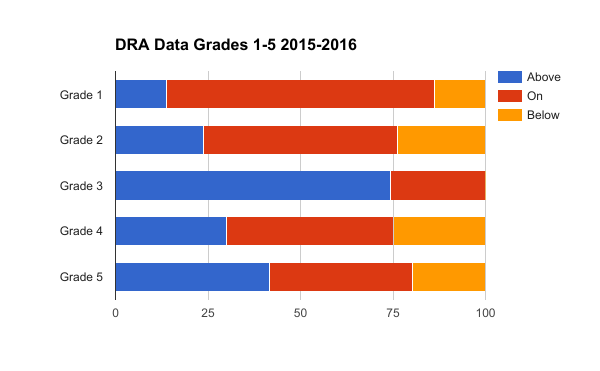
\includegraphics[width=\textwidth]{profile16}
\caption{DRA Data Grades 1, 2, 4, and 5 2015-2016}
\end{figure}

\subsection{International Schools’ Assessment (ISA)}

Historically, CMIS has given the \href{https://drive.google.com/drive/u/0/folders/0B71_pYxcTLo-anRvTzA5NDBGUW8}{ACER ISA} (International Schools’ Assessment) test to students in grades 3, 5, and 7.  Data from these tests show CMIS students performing as well as or better than both “All Students” taking the ACER ISA and students categorized in “comparable schools” with the same percentage of students from an English-speaking background.  Comparisons were done using the Student’s t-test. 

\begin{table}
\caption{English Speaking Background}
\label{table:10}
\begin{tabu}{|c|X|c|}
\hline
Academic Year &
CMIS \% of English Background Speakers &
ISA Group \\
\hline
2011-2012  &
41 to 55\% &
3 \\
\hline
2012-2013  &
26 to 40\% &
2 \\
\hline
2013-2014  &
26 to 40\% &
2 \\
\hline
2014-2015  &
41 to 55\% &
3 \\
\hline
2015-2016  &
36 to 55\% &
3 \\
\hline
\end{tabu}
\end{table}

Based on our reported percentage of students from an English-speaking background, CMIS is categorized differently by ISA each year.  For example, in the 2011-1012 academic year, CMIS was initially categorized in ISA Group 3.  However, from 2012 to 2014, CMIS demographics shifted to 26 to 40\% of students from an English speaking background, placing us in ISA Group 2.  In the 2014-2015 academic year, the percentage of CMIS English background students increased to 41 to 55\%, shifting us into ISA Group 3.  In the 2015-2016 academic year, while the percentage of CMIS English background students fluctuated from 36 to 55\%, we remained within the range of ISA Group 3.  Thus, a year by year comparison with comparable schools is hard to make and interpret.  For an individual student taking the test in Grades 3, 5, and 7, a comparison is made to students in schools with different demographics.  Because the ranking of an individual student changes with the respective ISA Group, it is impossible to see relative progress over time.  

During the Data Wise initiative 2015-2016, a study of the ISA data identified the need for students to further develop their Expository/Argumentative Writing skills.  A \href{https://drive.google.com/drive/folders/0ByVFfrm0zfolLU9Vb0ZBeF9uZjQ}{school wide writing assessment} was given to further confirm this need, and an action plan was created to scaffold the students that needed extra attention with this particular skill. Tools such as graphic organizers were created and placed in classrooms.  We also created a \href{https://docs.google.com/document/d/1JvVcmrIylkSYJeT4vgbyrqQTfZuJW-Iu6GB6jNCreIU/edit?ts=58a5129f}{common assessment rubric for English Language Arts (ELA) 9-12}.  Using Acer ISA in Datawise was challenging for the following reasons: 
\begin{itemize}
\item the category of schools CMIS falls into changes based on the percentage of students from an English-speaking background, thus making a year by year comparison difficult.
\item The Standards addressed in the ISA tests were not the same standards used at CMIS.
\item Students are tested in grades 3, 5, and 7.  The long time interval between tests does not support modifying instruction to fit student needs.
\end{itemize}

\begin{table}
\caption{Average ISA Test Results (Grade 3), 2011-2016}
\label{table:11}
\begin{tabu}{|X[2]|X|X|X|X|X|}
\hline
  &
2011-12 &
2012-13 &
2013-14 &
2014-15 &
2015-16 \\
\hline
\multicolumn{6}{|l|}{Mathematical Literacy} \\
\hline
CMIS &
315 &
365 &
334 &
344 &
327 \\
\hline
All Schools  &
310 &
334 &
308 &
330 &
327 \\
\hline
\multicolumn{6}{|l|}{Reading} \\
\hline
CMIS  &
263 &
293 &
292 &
323 &
319 \\
\hline
All Schools  &
254 &
255 &
266 &
291 &
257 \\
\hline
\multicolumn{6}{|l|}{Writing A} \\
\hline
CMIS  &
381 &
374 &
409 &
367 &
377 \\
\hline
All Schools  &
375 &
364 &
378 &
378 &
363 \\
\hline
\multicolumn{6}{|l|}{Writing B}\\
\hline
CMIS  &
405 &
396 &
430 &
407 &
389 \\
\hline
All Schools  &
392 &
395 &
409 &
413 &
391 \\
\hline
\end{tabu}
\end{table}

\begin{figure}
\centering
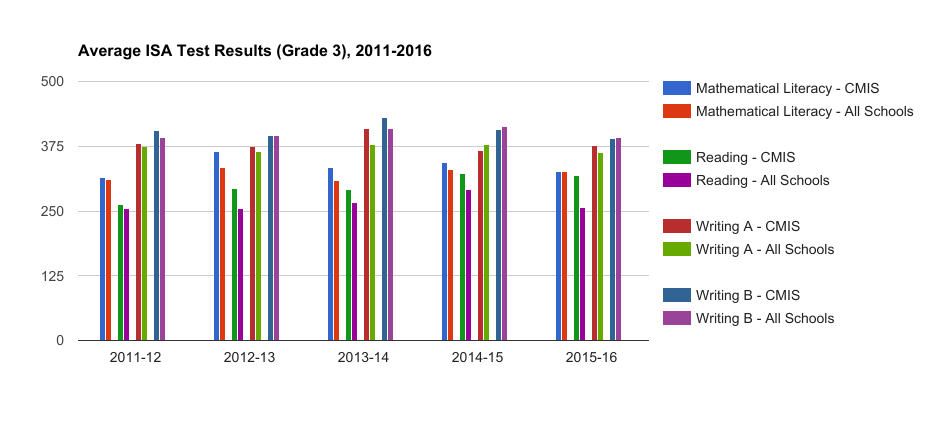
\includegraphics[width=\textwidth]{profile17}
\caption{Average ISA Test Results (Grade 3) 2011-2016}
\end{figure}

\begin{figure}
\centering
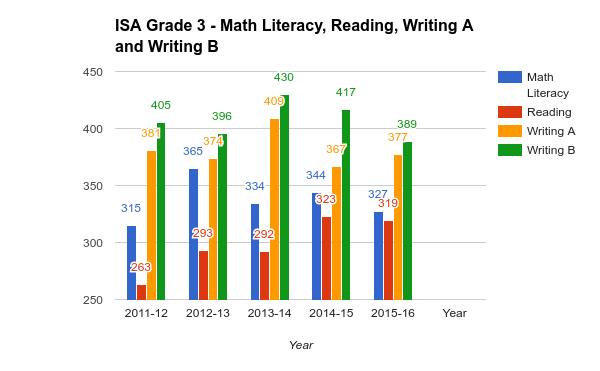
\includegraphics[width=\textwidth]{profile18}
\caption{ISA Grade 3 - Math Literacy, Reading, Writing A and Writing B}
\end{figure}

\begin{table}
\caption{Average ISA Test Results (Grade 5), 2011-2016}
\label{table:12}
\begin{tabu}{|X[2]|X|X|X|X|X|}
\hline
&
2011-12  &
2012-13 &
2013-14 &
2014-15 &
2015-16 \\
\hline
\multicolumn{6}{|l|}{Mathematical Literacy} \\
\hline
CMIS  &
444 &
486 &
471 &
458 &
449 \\
\hline
All Schools  &
417 &
424 &
432 &
444 &
427 \\
\hline
\multicolumn{6}{|l|}{Reading} \\
\hline
CMIS  &
432 &
412 &
385 &
460 &
441 \\
\hline
All Schools  &
381 &
357 &
362 &
396 &
361 \\
\hline
\multicolumn{6}{|l|}{Writing A} \\
\hline
CMIS  &
494 &
486 &
472 &
475 &
486 \\
\hline
All Schools  &
455 &
451 &
461 &
460 &
455 \\
\hline
\multicolumn{6}{|l|}{Writing B} \\
\hline
CMIS  &
487 &
498 &
484 &
487 &
513 \\
\hline
All Schools  &
465 &
467 &
487 &
482 &
467 \\
\hline
\end{tabu}
\end{table}

\begin{figure}
\centering
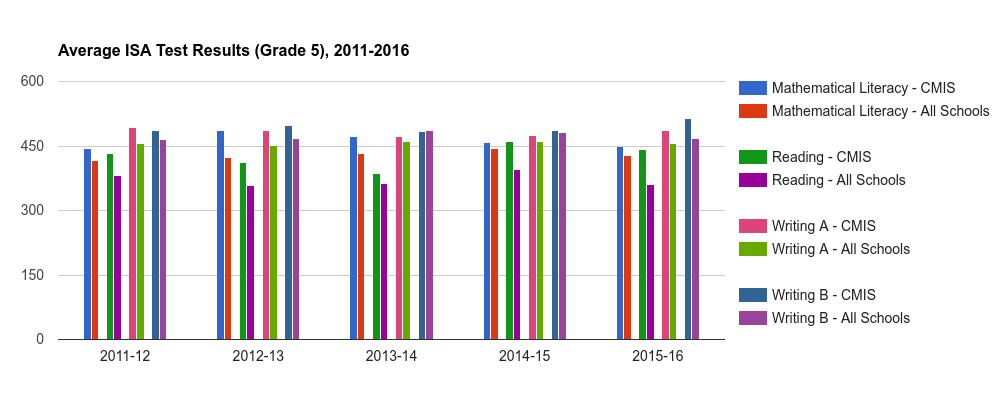
\includegraphics[width=\textwidth]{profile19}
\caption{Average ISA Test Results (Grade 5), 2011-2016}
\end{figure}

\begin{figure}
\centering
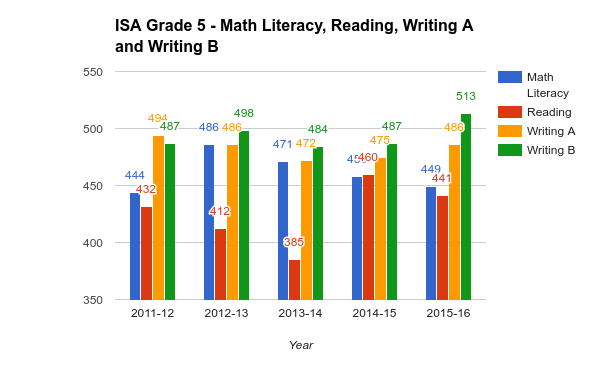
\includegraphics[width=\textwidth]{profile20}
\caption{ISA Grade 5 - Math Literacy, Reading, Writing A and Writing B}
\end{figure}

\begin{table}
\caption{Average ISA Test Results (Grade 7), 2011-2016}
\label{table:11}
\begin{tabu}{|X[2]|X|X|X|X|X|}
\hline
  &
2011-12 &
2012-13 &
2013-14 &
2014-15 &
2015-16 \\
\hline
\multicolumn{6}{|l|}{Mathematical Literacy} \\
\hline
CMIS  &
534 &
582 &
559 &
545 &
526 \\
\hline
All Schools  &
486 &
504 &
521 &
512 &
507 \\
\hline
\multicolumn{6}{|l|}{Reading} \\
\hline
CMIS  &
526 &
515 &
500 &
504 &
495 \\
\hline
All Schools  &
454 &
447 &
451 &
448 &
457 \\
\hline
\multicolumn{6}{|l|}{Writing A} \\
\hline
CMIS  &
553 &
550 &
546 &
569 &
526 \\
\hline
All Schools  &
512 &
511 &
525 &
526 &
517 \\
\hline
\multicolumn{6}{|l|}{Writing B} \\
\hline
CMIS  &
531 &
550 &
528 &
534 &
541 \\
\hline
All Schools  &
518 &
523 &
540 &
533 &
525 \\
\hline
\end{tabu}
\end{table}

\begin{figure}
\centering
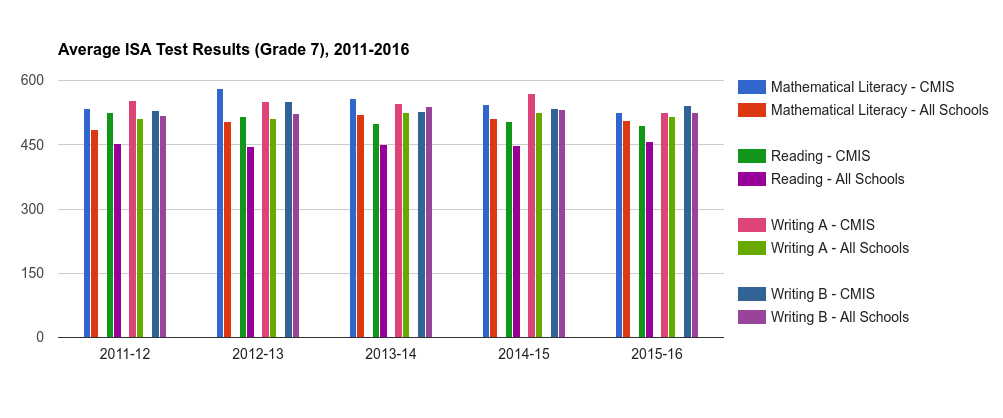
\includegraphics[width=\textwidth]{profile21}
\caption{Average ISA Test Results (Grade 7), 2011-2016}
\end{figure}

\begin{figure}
\centering
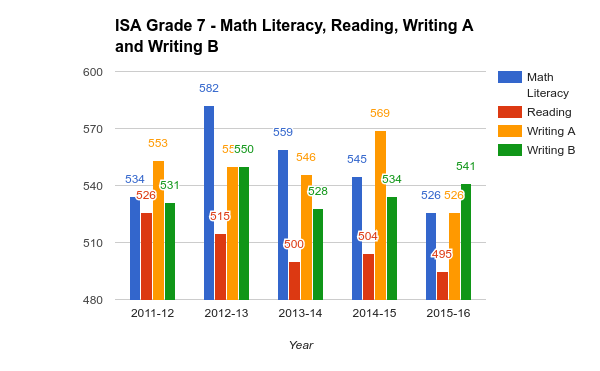
\includegraphics[width=\textwidth]{profile22}
\caption{ISA Grade 7 - Math Literacy, Reading, Writing A and Writing B}
\end{figure}

\subsection{Northwest Evaluation Association (NWEA) Measures of Academic Progress (MAP)}

CMIS has re-adopted the NWEA MAP (Measures of Academic Progress) test, starting in January 2017. (It was previously used in the 2011-2012 academic year.)  School Administrators anticipate that MAP will provide more useful data, as each student in Gr. 2-10 will be tested twice annually.  MAP tests are based on the Common Core objectives for each respective grade level.  

\subsection{PSAT 8/9}

All students in grades 8 and 9 take the Practice Scholastic Aptitude Test 8/9 (PSAT 8/9) in October, in accordance with the dates set by the College Board. According to the global data compared with the random selection of PSAT results from around the world, the majority of CMIS students perform better than the mean. In general CMIS students excel on these tests.   PSAT test-takers receive a copy of their results and are asked to use them to help target areas where they need improvement.  

The scores for the\href{https://docs.google.com/a/cmis.ac.th/spreadsheets/d/1OVMnw4x1eUg-QByMt2J2IZJkovZGys_8uoj1SKSM2As/edit?usp=sharing}{ first two years for the PSAT 8/9 (2015-17)} are shown below as compared to a sample of n=1,000 for the PSAT 8/9.  Center lines show the medians; box limits indicate the 25th and 75th percentiles as determined by R software; whiskers extend 1.5 times the interquartile range from the 25th and 75th percentiles, outliers are represented by dots; crosses represent sample means. Blue indicates grade 8, yellow is grade 9, and green represents the combined score of grades 8 and 9.  

With the exception of outliers, almost all CMIS students tested scored above the median score of the sample group.  

\begin{figure}
\centering
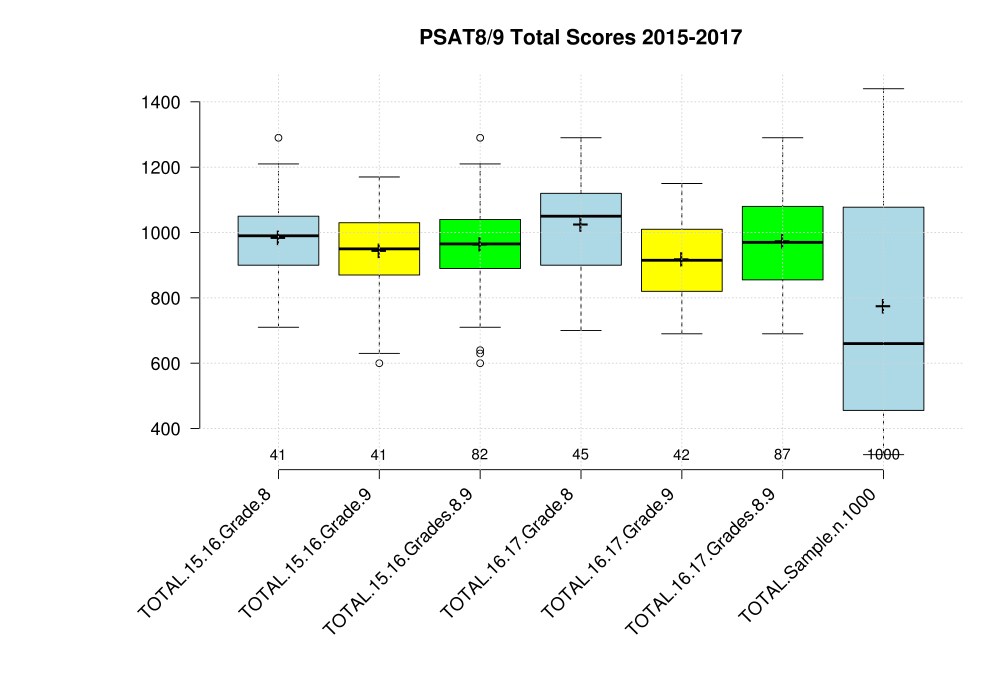
\includegraphics[width=\textwidth]{profile23}
\caption{PSAT8/9 Total Scores 2015-2017}
\end{figure}

\begin{figure}
\centering
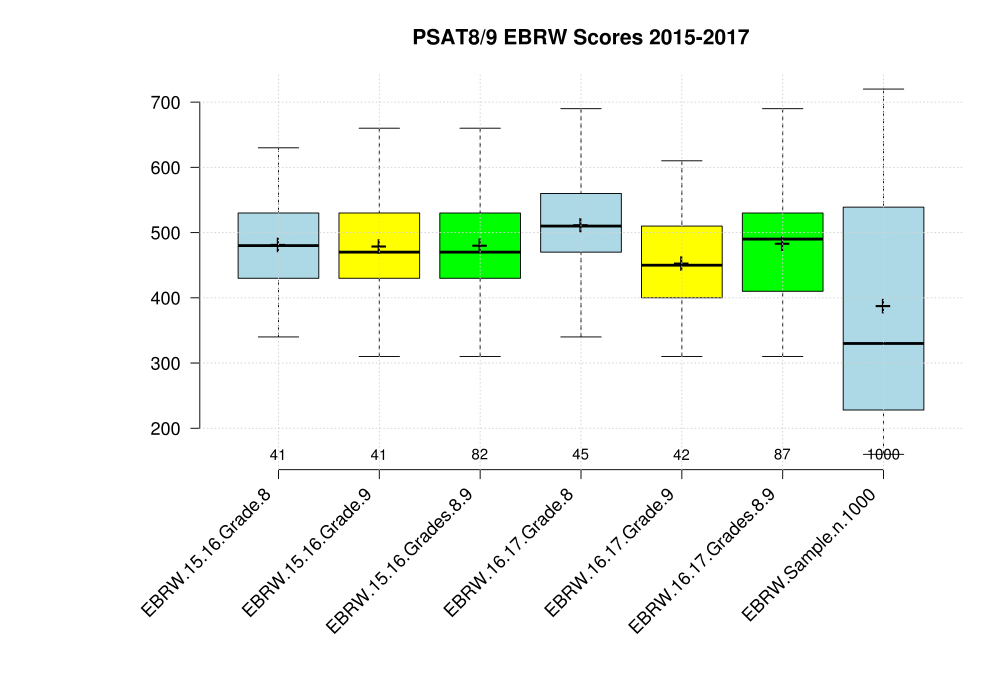
\includegraphics[width=\textwidth]{profile24}
\caption{PSAT8/9 EBRW Scores 2015-2017}
\end{figure}

\begin{figure}
\centering
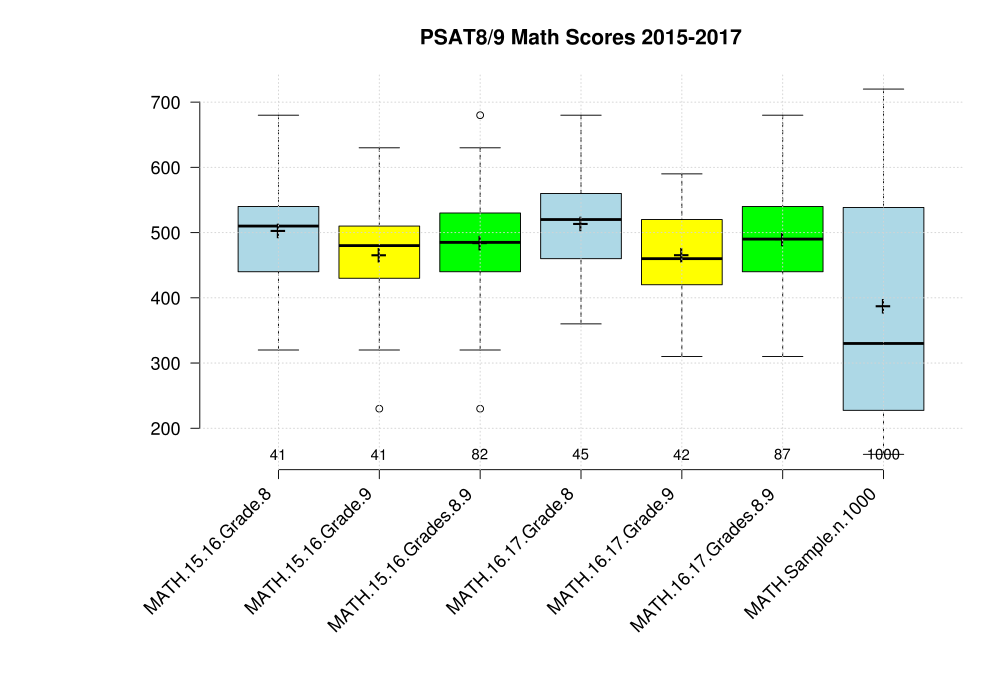
\includegraphics[width=\textwidth]{profile25}
\caption{PSAT8/9 Math Scores 2015-2017}
\end{figure}

\subsection{PSAT/NMSQT}

Students in grades 10 and 11 take the Preliminary Scholastic Aptitude Test\href{https://drive.google.com/drive/folders/0B71\_pYxcTLo-VGNkQlZtTFlIQlE}{ (PSAT) / National Merit Scholarship Qualifying Test (NMSQT)} in October, in accordance with the dates set by the College Board. According to the global data compared with the random selection of PSAT results from around the world, the majority of CMIS students perform better than the mean. In general, CMIS students excel on these tests.  In fact, one of our students was nominated for the National Merit Scholarship Award by scoring in the top 5\% of all PSAT test-takers in 2015.  PSAT test-takers receive a copy of their results to help target areas where they need to improve before taking the SAT exam.  

\minor{\href{https://collegereadiness.collegeboard.org/about/scores/benchmarks}{Benchmark Indicators}}

Score reports use colors to show how students’ section scores relate to the SAT or grade-level benchmark.
\begin{itemize}
\item Green: The section score meets or exceeds the benchmark.
\item Yellow: The section score is within one year’s academic growth of the benchmark.
\item Red: The section score is below the benchmark by more than one year’s academic growth.
\end{itemize}

\minor{SAT College and Career Readiness Benchmarks}

Evidence-Based Reading and Writing: 480

Math: 530

SAT Section Score Ranges

200-800 Point Scale
 
\begin{tabular}{|l|c|c|c|}
\hline
  &
Red &
Yellow &
Green \\
\hline
Evidence-Based  
Reading and Writing &
200-450 &
460-470 &
480-800 \\
\hline
Math  &
200-500 &
510-520 &
530-800 \\
\hline
\end{tabular}

\minor{11th Grade Benchmarks}

Evidence-Based Reading and Writing: 460

Math: 510

11th Grade Section Score Ranges

160-760 Point Scale

\begin{tabular}{|l|c|c|c|} 
\hline
  &
Red &
Yellow &
Green \\
\hline
Evidence-Based
Reading and Writing  &
160-420 &
430-450 &
460-760 \\
\hline
Math  &
160-470 &
480-500 &
510-760 \\
\hline
\end{tabular}


\minor{10th Grade Benchmarks}


Evidence-Based Reading and Writing: 430

Math: 480

10th Grade Section Score Ranges
 
160-760 Point Scale

\begin{tabular}{|l|c|c|c|} 
\hline
  &
Red &
Yellow &
Green \\
\hline
Evidence-Based
Reading and Writing  &
160-400 &
410-420 &
430-760 \\
\hline
Math  &
160-440 &
450-470 &
480-760 \\
\hline
\end{tabular}



\begin{table}[h]
\caption{2015-2016 PSAT/NMSQT Scores compared with all students taking PSAT/NMSQT}
\label{table:12}
\begin{tabu}{|X|X|X|X|X|X|X|X|}
\hline
Year &
Grade &
\# Students &
School &
Met Both &
Met EBRW &
Met Math &
Met None \\
\hline
2015-16 &
10 &
40 &
CMIS &
68\% &
88\% &
73\% &
8\% \\
\hline
2015-16 &
10 &
 &
All &
39\% &
63\% &
43\% &
33\% \\
\hline
2015-16 &
11 &
41 &
CMIS &
76\% &
95\% &
80\% &
0\% \\
\hline
2015-16 &
11 &
 &
All &
42\% &
67\% &
45\% &
30\% \\
\hline
2016-17 &
10 &
39 &
CMIS &
72\% &
92\% &
77\% &
3\% \\
\hline
2016-17 &
10 &
 &
All &
40\% &
64\% &
43\% &
33\% \\
\hline
2016-17 &
11 &
34 &
CMIS &
85\% &
97\% &
85\% &
3\% \\
\hline
2016-17 &
11 &
 &
All &
46\% &
69\% &
48\% &
29\% \\
\hline
\end{tabu}
\end{table}

\begin{figure}
\centering
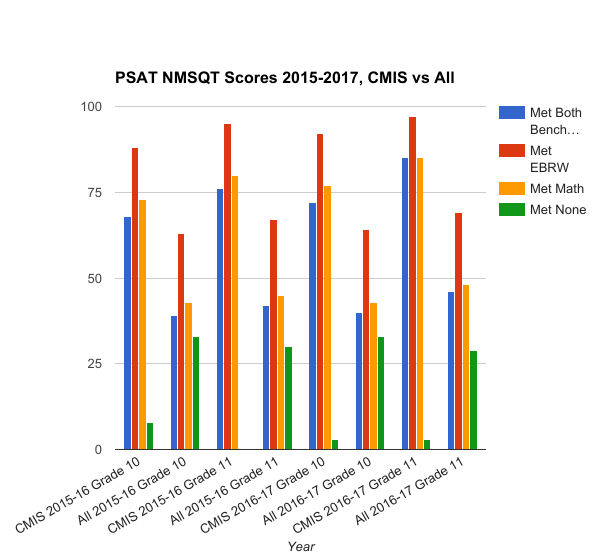
\includegraphics[width=\textwidth]{profile26}
\caption{PSAT NMSQT 2015-2017, CMIS vs All}
\end{figure}

\begin{figure}
\centering
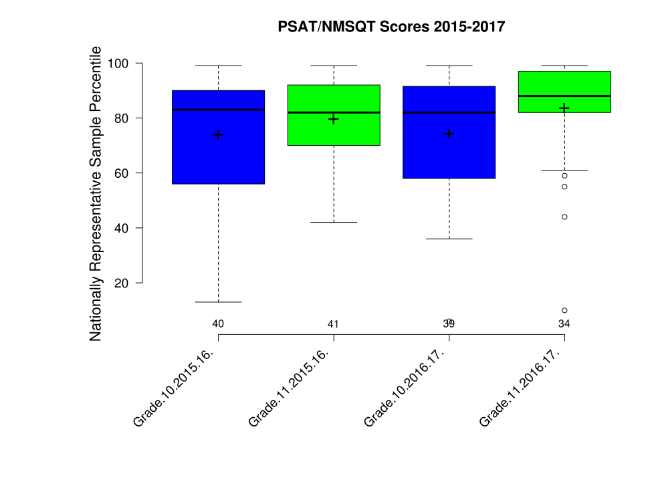
\includegraphics[width=\textwidth]{profile27}
\caption{PSAT/NMSQT Scores 2015-2017}
\end{figure}

\subsection{Scholastic Aptitude Test (SAT)}

CMIS students take the Scholastic Aptitude Test (SAT) in grades 11 and 12.  According to the \href{https://www.prepscholar.com/sat/s/}{prep scholar website} a good score for a college-bound student is at or above 1,000.  An excellent score (top 25\%) falls at or above 1,200.  For the past five years, the average mean score of CMIS SAT-takers has fallen within the range of college-bound students.  (The data from 2015 and earlier has been adjusted using the College Board’s Concordance table.)

\begin{figure}
\centering
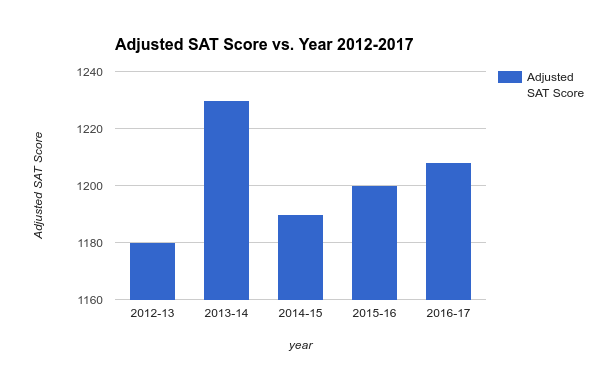
\includegraphics[width=\textwidth]{profile28}
\caption{Adjusted SAT Score vs. Year 2012-2017}
\end{figure}

\subsection{AP Courses}

CMIS has offered a variety of AP course for over 12 years. Students are allowed to enroll in an AP course if they complete the prerequisite courses and obtain teacher approval.  CMIS students who take AP courses historically do very well and score well above the global average, as well the average for international schools in Thailand.  However, CMIS students have the option taking the AP course without taking the AP exam, so many students only choose to take exams for which they feel well prepared.  Over the past 5 years, the AP program at CMIS has increased its course offerings to 19 different courses, and student participation has increased over the past 2 years.

\begin{figure}
\centering
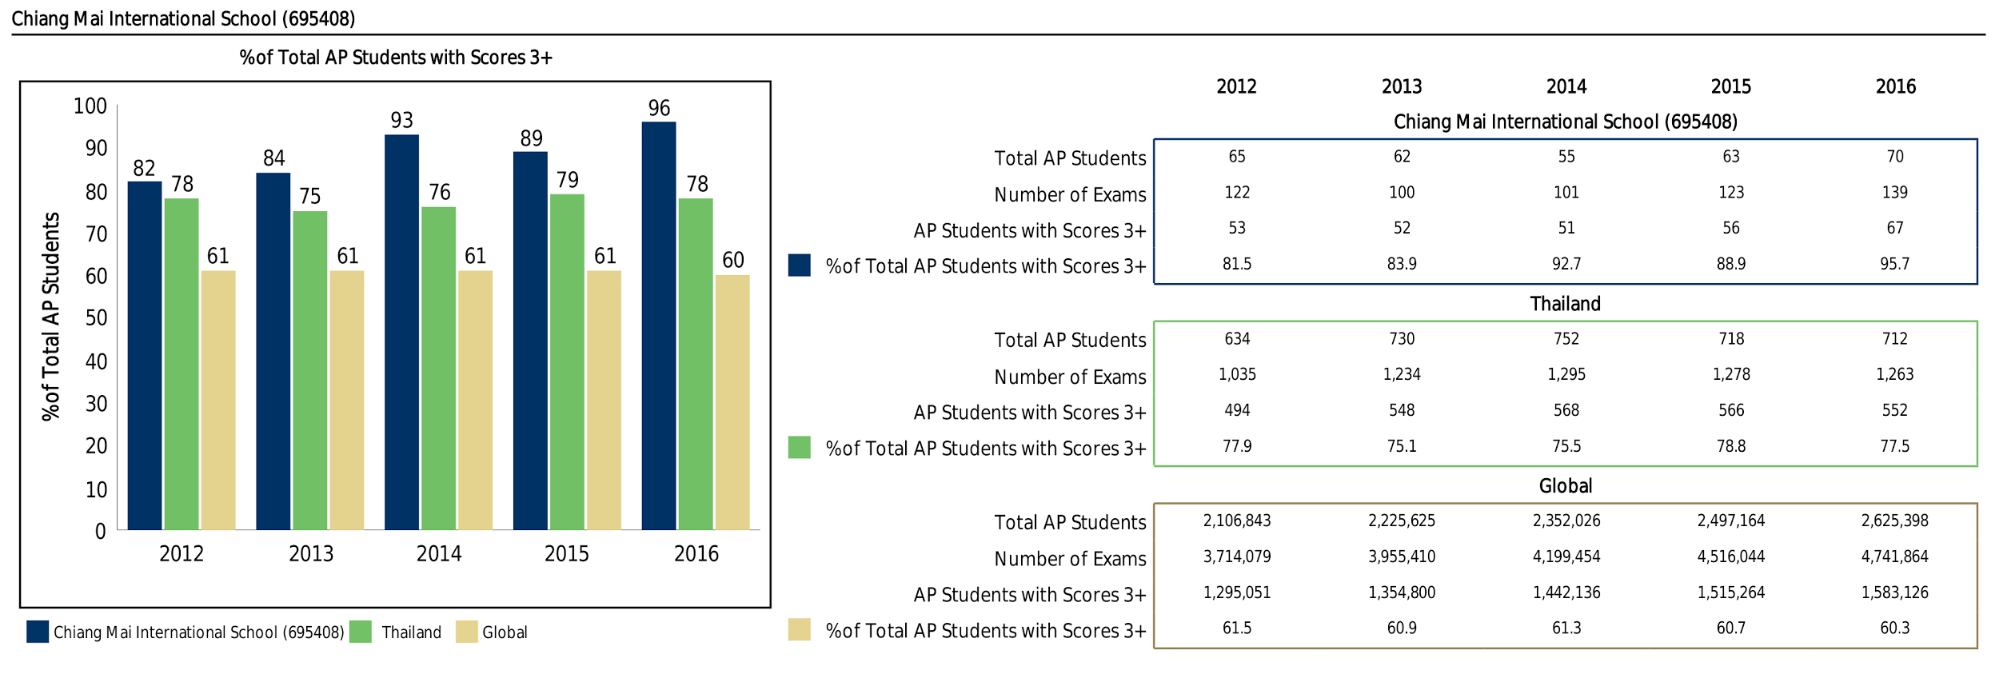
\includegraphics[width=\textwidth]{profile29}
\caption{AP Exam Score Summary}
\end{figure}

\subsection{Students Plans Post Graduation}

College planning for CMIS students begins in Gr. 10.  All Gr. 10 students are required to take the PSAT (Preliminary Scholastic Aptitude Test), and the SAT (Scholastic Aptitude Test) before completion of Gr. 12.  The CMIS College Guidance Counselor works with all eligible students in identifying their options, exploring their possibilities, and planning their applications to colleges and universities.  High school students have been given Overgrad accounts to help track and research interests in careers and universities, mostly in the United States.  

\minor{University Entrance}

\begin{table}
\caption{Post-graduation Plans}
\label{table:13}
\begin{tabu}{|X|X|X|X|X|X|}
\hline
Year &
Number of Seniors &
Enter College/University &
Gap Year &
Did not enter College/University &
\%Matriculating \\
\hline
2015-16 &
37 &
36 &
1 &
0 &
100\% \\
\hline
2014-15 &
36 &
32 &
4 &
0 &
100\% \\
\hline
2013-14 &
40 &
36 &
4 &
0 &
100\% \\
\hline
\end{tabu}
\end{table}

CMIS graduates gain admission to colleges and universities around the world, with many electing to study in North America. Approximately 98\% of CMIS students attend post­-secondary institutions upon graduation. The following is a list of colleges and universities to which CMIS Class of 2015 graduates were offered acceptance.  This information is generally included in our School Profile.

\minor{\href{https://docs.google.com/document/d/1i8tDt8omsO9Zz4Zj40uOpUz8twkbGHYSk_PDs3Rqup4/edit}{Class of 2015-16 College and University Placement}}

In recent years, CMIS graduates have been accepted to a wide variety of international colleges and universities, as listed below. In keeping with this tradition of excellence, students in our 2015 graduating class have been offered acceptance into an impressive array of colleges and universities throughout the world. Those universities in which our current graduates have been offered acceptance are indicated with an asterisk. 

\begin{itemize}
\item Baylor University, Waco, TX
\item *Bentley University, Waltham, MA
\item Boston University, Boston, MA
\item Biola University, La Mirada, CA
\item *Bryn Mawr College, Bryn Mawr, PA
\item *California Polytechnic State University, San Luis Obispo, CA
\item California State University Fullerton, Fullerton, CA
\item *Calvin College, Grand Rapids, MI
\item *Carroll College, Waukesha, WI
\item Clark University, Worcester, MA
\item *Cornell University, Ithaca, NY
\item Davidson College, Davidson, NC
\item Emory University, Atlanta, GA
\item Fordham University, Bronx, NY
\item *Grinnell College, Grinnell, IA
\item *Hult, International Business School, Boston, MA
\item *Ithaca College, New York, NY
\item Lancaster Bible College, Lancaster, PA
\item Lafayette College, Easton, PA
\item Lewis and Clark College, Portland, OR
\item Marquette University, Milwaukee, WI
\item *Messiah College, Mechanicsburg, PA
\item Michigan State University, East Lansing, MI
\item Mississippi State University, MS
\item *Mount Holyoke College, South Hadley, MA
\item *New York University, Greenwich Village, NY
\item *Northeastern University, Boston, MA
\item Ohio Wesleyan University, Delaware, OH
\item Penn State University, State College, PA
\item Purdue University, West Lafayette, IN
\item Rochester Institute of Technology, Rochester, NY
\item Rutgers University, New Brunswick, NJ
\item Rice university, Houston, TX
\item Savannah College of Art and Design (SCAD), Savannah, GA
\item State University of New York, (SUNY), Buffalo, NY
\item Syracuse University, Syracuse, NY
\item Texas A\&M University, College Station, TX
\item *University of Akron, Akron, OH
\item *University of California, Irvine / Davis / Riverside, CA
\item *University of Connecticut, Storrs, CT
\item *University of Illinois Urbana Champaign, Champaign, IL
\item *University of Massachusetts, Amherst, MA
\item *University of Michigan, Ann Arbor, MI
\item University of San Francisco, San Francisco, CA
\item University of Washington, Seattle, WA
\item Vanderbilt University, Nashville, TN
\item Virginia Polytechnic Institute, Blacksburg, VA
\item *Wheaton College, Wheaton, IL
\end{itemize}


Canada:

\begin{itemize}
\item Carleton University, Ottawa, Ontario
\item *Trinity Western University, BC
\item University of British Columbia, Vancouver, BC
\item * University of Toronto
\item *University of Waterloo, Toronto
\end{itemize}


Europe:

\begin{itemize}
\item *Ecole hoteliere de Lausanne, Lausanne, Switzerland
\item *Eindhoven University of Technology, Netherlands
\item Erasmus University College, Rotterdam, Netherlands
\item *Hague University of Applied Science, Netherlands
\item *Hanze University, Groningen, Netherlands
\item University College Roosevelt, Middelburg, Zeeland, Netherlands
\item University of Groningen (RUG), Groningen, Netherlands
\item *University of Aberdeen, Scotland, UK
\item *University of Nottingham, England, UK
\item *University of Sheffield, England, UK
\item *University of Stirling, Scotland, UK
\item *University of Strathclyde, Scotland, UK
\end{itemize}

Australia:

\begin{itemize}
\item *Le Cordon Bleu, Culinary Arts Institute, Sydney
\item *Blue Mountains, International Hotel Management School, Sydney
\end{itemize}


Thailand:

\begin{itemize}
\item *Assumption, University, (ABAC), Bangkok
\item *Chulalongkorn University, Bangkok
\item *Mahidol University, Bangkok
\item Payap University, Chiang Mai
\item *Thammasat University, Bangkok
\end{itemize}


Other Parts of Asia:

\begin{itemize}
\item *Ritsumeikan Asia Pacific University, Oita, Japan
\item *Nanyang Technological University, Singapore
\item *Shanghai Jiao Tong University, Shanghai, China
\item *State University of New York (SUNY), Seoul, Korea
\end{itemize}


\tcbsection{School Community Surveys (Teacher, Student, Community}

Every academic year, in May, CMIS sends out opinion surveys to the community.  Results from the surveys provide data regarding community perception in the areas of curriculum, learning, and school environment. 

The demographic groups surveyed are: teachers and staff, students grade 4-12, and CMIS Families. The questions in each survey are targeted to the corresponding demographic group. In order to capture data from our entire community, the CMIS Family survey is provided in English, Korean, and Thai (the three major segments of the student/family population).

Administration review the survey data and use responses to guide planning and target areas for improvement.

\subsection{Teacher Survey}

At the beginning of the 2016-17 school year the Administrative Team (principals and superintendent) analyzed the 2015-16 CMIS staff survey together and identified two items for improvement:
\begin{itemize}
\item My administrator knows what is going on in my classroom.
\item If I am feeling stressed out or overloaded, I feel comfortable talking to my division administrator. 
\end{itemize}


During the September professional development early dismissal day, the administrative team shared the areas with the staff and asked for anonymous suggestions of ways to improve. From these suggestions came the following three initiatives:
\begin{itemize}
\item A weekly schedule of classroom walkthroughs by principals, PK-12.  The schedule provides consistency and helps address the the issue of “My administrator knows what is going on in my classroom”.
\item Principals and Superintendent visible and available on the playground every day before school starts.  This opportunity provides a personal opportunity for staff to easily locate and approach the administrative team.
\item Department Check-Ins completed by the Superintendent (via-email or during Team Leader meetings), where team leaders are asked to identify the needs of their team and encouraged to share ideas of how the Administrative Team can best support them.
\end{itemize}

The Administrative Team will complete a brief staff survey in February as a way to assess perceptions of the above initiatives.  A Summary of CMIS Staff Survey \ref{table:14} results is included below.   


\begin{figure}
\centering
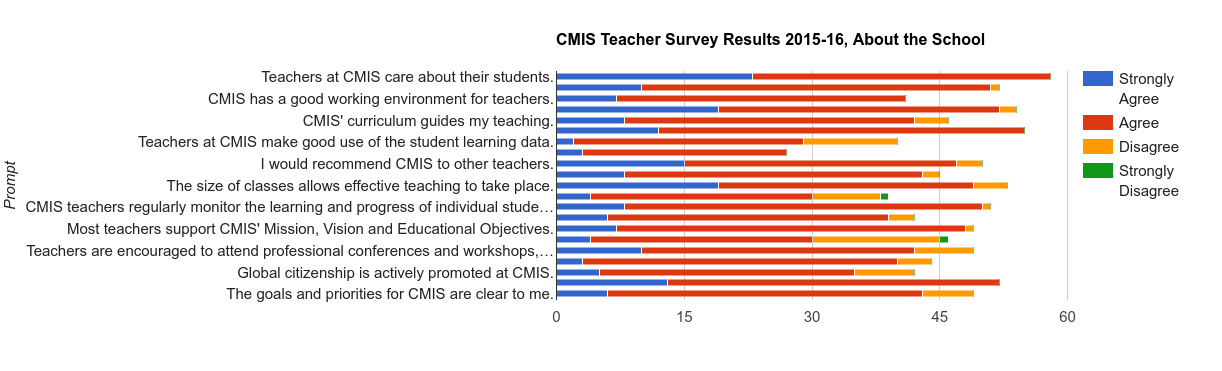
\includegraphics[width=\textwidth]{profile30}
\caption{CMIS Teacher Survey Results 2015-2016, About the School}
\end{figure}

\begin{figure}
\centering
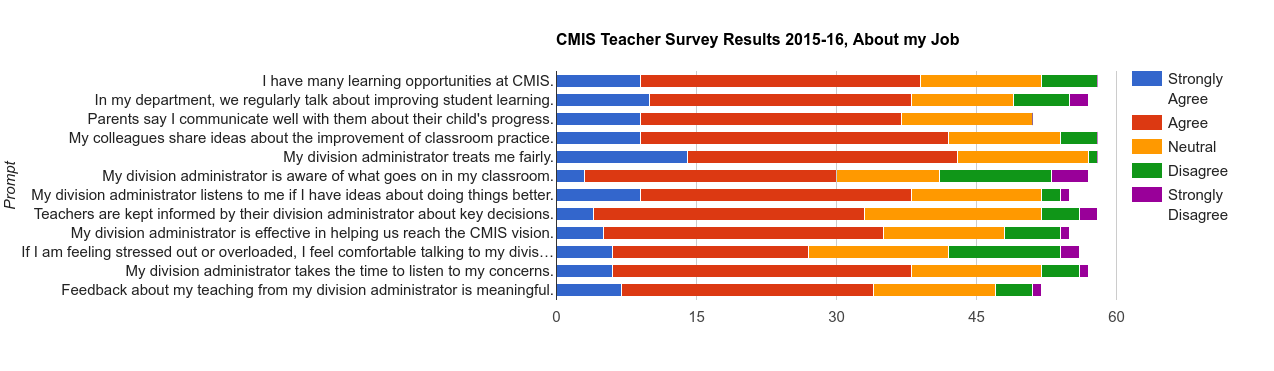
\includegraphics[width=\textwidth]{profile31}
\caption{CMIS Teacher Survey Results 2015-2016, About my Job}
\end{figure}

\begin{figure}
\centering
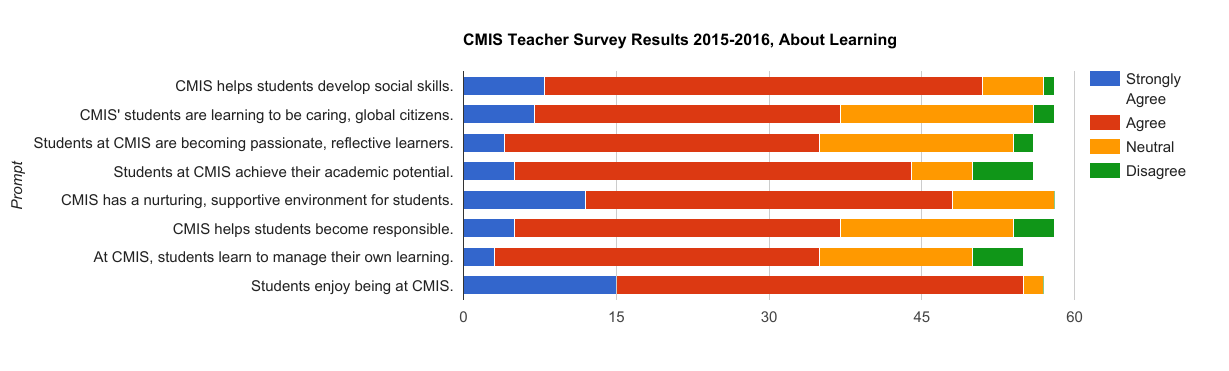
\includegraphics[width=\textwidth]{profile32}
\caption{CMIS Teacher Survey Results, About Learning}
\end{figure}

\subsection{Family Survey}

During the 2016 Board retreat, the Board analyzed the\href{https://docs.google.com/a/cmis.ac.th/forms/d/16Gbd3MzQOXtjjZ2dG460xw5SHG_eohMIKet3lxYUdAY/edit#responses}{ 2015-16 CMIS Family Survey} and identified two areas for improvement:
\begin{itemize}
\item Communication
\item Who does what, roles of the CMIS board members
\end{itemize}


These items are addressed by the following initiatives:
\begin{itemize}
\item Creating a forum where the \href{https://docs.google.com/document/d/1kiwakkg8eKdtEexCxVNx-m1CfC3VqxhukDy8WXDPGKY/edit?ts=58a2a142}{community determines what is presented} during the PTG meetings. Instead of the school driving the content presented to the community during these meetings, PTG meetings are driven by what the community wants. For example, topics such as college and career counseling, technology use, student activities, student health with regard to Chiang Mai’s burning season, etc. have been recent topics identified by the community and discussed at PTG meetings.
\item What’s happening with the board? - CMIS board meeting summaries are created and posted on the CMIS PTG website, allowing more access and transparency to what is being discussed at the board level.
\item Who does what? - at least four CMIS board members attend every PTG meeting, these members are identified so that parents have a greater sense of who is on the CMIS board. CMIS board members attend and speak at CMIS events whenever possible, for example, back-to-school bbq, CMIS Christmas Concert, CMIS Plays, CMIS Latin Night, etc. Additionally, CMIS board members, the roles and responsibilities of the board and it’s individual members will be displayed on the CMIS website.
\end{itemize}

The Board will follow up with a community, “Sounding Board” session in March 2017 as an informal way to assess perceptions of the above initiatives.  A \href{https://docs.google.com/a/cmis.ac.th/document/d/1_otvw47y3Z-1CSjXnKhgRTauVRqPl1S6nSdmsb00O2k/edit?usp=sharing}{summary of the CMIS Family Survey} results is included in table \ref{table:14}:  

\begin{table}[h]
\tiny
\caption{Family Survey of Board/Leadership}
\label{table:14}
\tabulinesep=^2pt_2pt
\begin{longtabu}{|X[8]|X|X|}
\hline
Family Survey Questions related to Board/Leadership out of 127 responses &
\#/127 Agree &
\#/127 Disagree \\
\hline
The Board provides good representation for the CMIS community &
60 &
17 (13\%) \\
\hline
The Board makes decisions that help CMIS and plan for the future &
66 &
10 \\
\hline
The Board and school leadership execute responsible resource planning for the future &
61 &
16 (13\%) \\
\hline
The Board encourages suggestions and feedback about improving CMIS &
62 &
19 (15\%) \\
\hline
The Board works actively to improve CMIS &
64 &
14 (11\%) \\
\hline
The Board models the qualities of respect, fairness, equity, integrity, and honesty in professional dealings with others. &
62 &
10 \\
\hline
The Board communicates effectively with the CMIS community &
57 &
21 (17\%) \\
\hline
The Board respects diversity, valuing people and cultures represented in the school and by the community at large. &
71 &
8 \\
\hline
The Director makes decisions that help CMIS and plan for the future &
61 &
5 \\
\hline
The Director and school leadership execute responsible resource planning for the future &
59 &
9 \\
\hline
The Director encourages suggestions and feedback about improving CMIS &
54 &
17 (13\%) \\
\hline
The Director works actively to improve CMIS &
59 &
8 \\
\hline
The Director communicates effectively with the CMIS community &
54 &
19 (15\%) \\
\hline
The Director models the qualities of respect, fairness, equity, integrity, and honesty in professional dealings with others. &
60 &
7 \\
\hline
The Director respects diversity, valuing people and cultures represented in the school and by the community at large. &
60 &
4 \\
\hline
The Manager makes decisions that help CMIS and plan for the future &
65 &
6 \\
\hline
The Manager and school leadership execute responsible resource planning for the future &
58 &
10 \\
\hline
The Manager encourages suggestions and feedback about improving CMIS &
59 &
12 \\
\hline
The Manager works actively to improve CMIS &
62 &
5 \\
\hline
The Manager communicates effectively with the CMIS community &
65 &
12 \\
\hline
The Manager models the qualities of respect, fairness, equity, integrity, and honesty in professional dealings with others. &
60 &
3 \\
\hline
The Manager respects diversity, valuing people and cultures represented in the school and by the community at large. &
61 &
3 \\
\hline
The Superintendent makes decisions that help CMIS and plan for the future &
77 &
4 \\
\hline
The Superintendent and school leadership execute responsible resource planning for the future &
75 &
5 \\
\hline
The Superintendent encourages suggestions and feedback about improving CMIS &
71 &
10 \\
\hline
The Superintendent works actively to improve CMIS &
75 &
4 \\
\hline
The Superintendent provides effective leadership for student achievement &
67 &
4 \\
\hline
The Superintendent provides effective leadership for appropriate student behaviour &
66 &
7 \\
\hline
The Superintendent provides effective leadership for teacher supervision (hiring, evaluation, etc.) &
64 &
8 \\
\hline
The Superintendent communicates effectively with the CMIS community &
73 &
7 \\
\hline
The Superintendent models the qualities of respect, fairness, equity, integrity, and honesty in professional dealings with others. &
72 &
2 \\
\hline
The Superintendent respects diversity, valuing people and cultures represented in the school and by the community at large. &
76 &
2 \\
\hline
The HS Principal provides effective leadership for student achievement &
39 &
3 \\
\hline
The HS Principal provides effective leadership for appropriate student behaviour &
38 &
7 \\
\hline
The HS Principal makes decisions that help CMIS and plan for the future &
41 &
3 \\
\hline
The HS Principal encourages suggestions and feedback about improving CMIS &
40 &
2 \\
\hline
The HS Principal works actively to improve CMIS &
40 &
2 \\
\hline
The HS Principal communicates effectively with the CMIS community &
41 &
2 \\
\hline
The HS Principal models the qualities of respect, fairness, equity, integrity, and honesty in professional dealings with others. &
40 &
4 \\
\hline
The HS Principal respects diversity, valuing people and cultures represented in the school and by the community at large. &
31 &
1 \\
\hline
The MS Principal provides effective leadership for student achievement &
45 &
4 \\
\hline
The MS Principal provides effective leadership for appropriate student behaviour &
46 &
2 \\
\hline
The MS Principal makes decisions that help CMIS and plan for the future &
44 &
3 \\
\hline
The MS Principal encourages suggestions and feedback about improving CMIS &
41 &
8 \\
\hline
The MS Principal works actively to improve CMIS &
46 &
4 \\
\hline
The MS Principal communicates effectively with the CMIS community &
43 &
6 \\
\hline
The MS Principal models the qualities of respect, fairness, equity, integrity, and honesty in professional dealings with others. &
44 &
4 \\
\hline
The MS Principal respects diversity, valuing people and cultures represented in the school and by the community at large. &
47 &
3 \\
\hline
The Elementary Principal makes decisions that help CMIS and plan for the future &
50 &
2 \\
\hline
The Elementary Principal encourages suggestions and feedback about improving CMIS &
49 &
5 \\
\hline
The Elementary Principal provides effective leadership for appropriate student behaviour &
52 &
4 \\
\hline
The Elementary Principal provides effective leadership for student achievement &
49 &
3 \\
\hline
The Elementary Principal works actively to improve CMIS &
50 &
3 \\
\hline
The Elementary Principal communicates effectively with the CMIS community &
48 &
5 \\
\hline
The Elementary Principal models the qualities of respect, fairness, equity, integrity, and honesty in professional dealings with others. &
49 &
4 \\
\hline
The Elementary Principal respects diversity, valuing people and cultures represented in the school and by the community at large. &
50 &
4 \\
\hline
\end{longtabu}
* Bolded items have more than a 10\% score of DISAGREE

English = 77 respondents
Thai = 39 respondents
Korean = 11 respondents
Total respondents = 127

Surveyed families represent the following students: 
ES respondents (children in PreK to G4) = 54
Grade 5 and MS (children in G5 to G8) = 68
HS respondents (children in G9 to G12) = 44
\end{table}


\subsection{\href{https://docs.google.com/a/cmis.ac.th/forms/d/1n7vFCQbPQmF6pEPJKPBsu4rzdiW4KQ_DrBcjTMUbLH4/viewanalytics}{Student Survey}}

In May 2016, students in grades 4 through 12 were given a student survey to gather perceptions on CMIS as a whole, their teachers, and their learning.  Below are the results of the 2015-2016 Student Survey.  

\begin{figure}
\centering
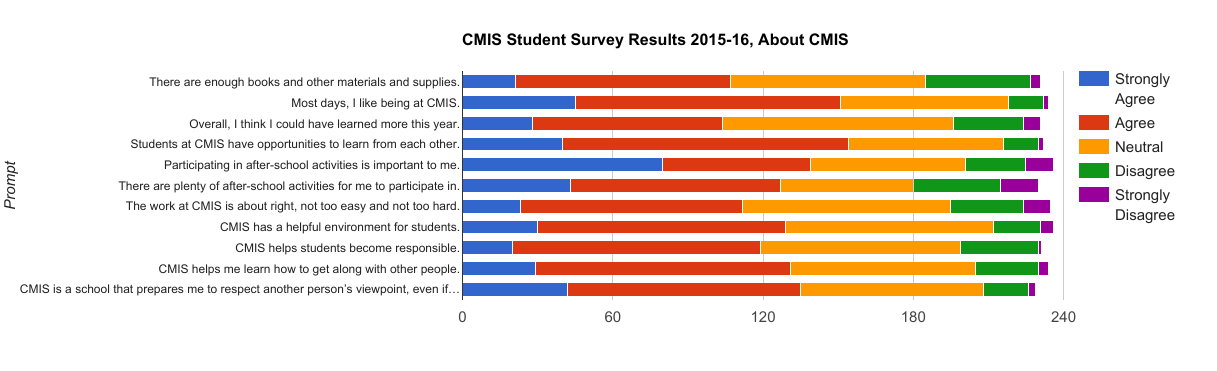
\includegraphics[width=\textwidth]{profile33}
\caption{CMIS Student Survey Results 2015-2016, About CMIS}
\end{figure}

\begin{figure}
\centering
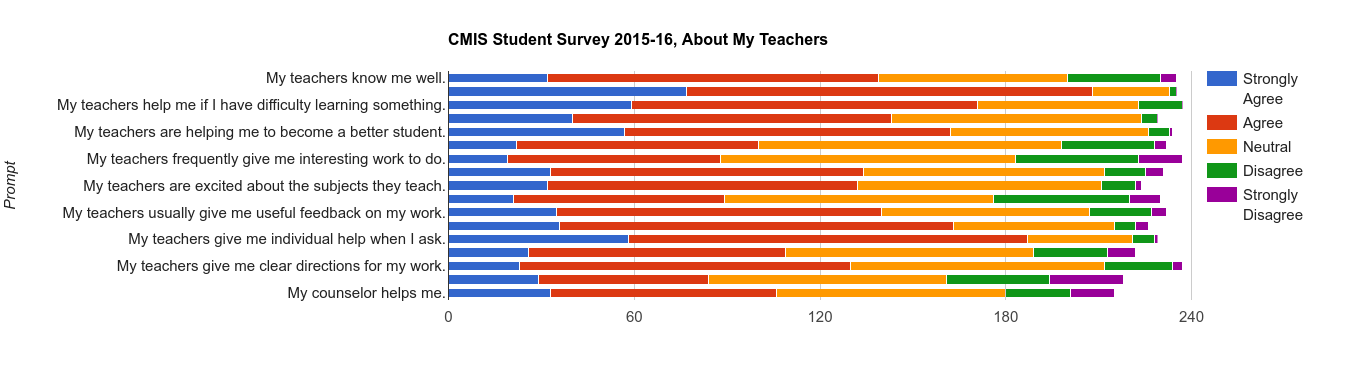
\includegraphics[width=\textwidth]{profile34}
\caption{CMIS Student Survey Results 2015-2016, About My Teachers}
\end{figure}

\begin{figure}
\centering
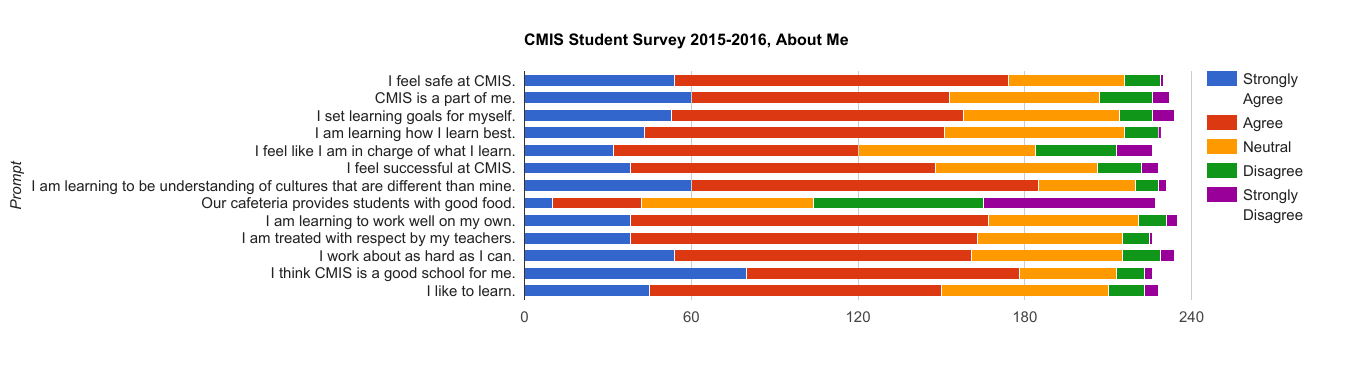
\includegraphics[width=\textwidth]{profile35}
\caption{CMIS Student Survey Results 2015-2016, About Me}
\end{figure}

At the beginning of the 2016-17 school year the SET (director, manager, superintendent) analyzed the 2015-16 CMIS Student Survey and identified two areas for improvement:
\begin{itemize}
\item School Cafeteria - food quality, price, and variety
\item Availability of student activities
\end{itemize}

\begin{figure}
\centering
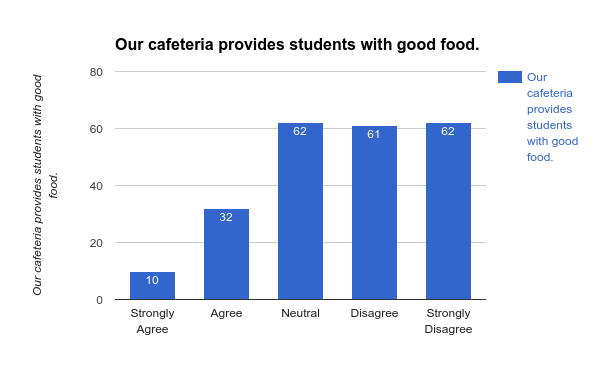
\includegraphics[width=\textwidth]{profile36}
\caption{Cafeteria Survey Results}
\end{figure}

\minor{Follow Up Cafeteria Survey}

To address the School Cafeteria concerns, a \href{https://docs.google.com/a/cmis.ac.th/forms/d/18wFe46SOpPVv9_jkKLEa4OqVsDkLtJkUCcM85Jul0Ik/viewanalytics}{survey} was constructed by the Health Officer and sent to all students. The purpose of the survey was to further identify issues existing with the school cafeteria. Actionable items resulting from the survey were: 

\begin{itemize}
\item Price 
\item Cafeteria lines
\item Availability of food (especially for MS/HS students)l
\item Variety of food available (especially for MS/HS students) 
\item Cafeteria design/size/temperature
\end{itemize}


The SET created a cafeteria committee who met with the contractors to discuss possible resolutions. As a result of this meeting:
\begin{itemize}
\item An increased variety of food is being offered
\item Snacks and pre made food  have been moved out of the cafeteria to improve the flow and shorten lines
\item Plans to expand the outdoor dining area and are now underway
\item Changes have been made to the new cafeteria building plans to address suggestions that came out of the survey 
\end{itemize}

The cafeteria committee will follow up with an additional survey to measure student perceptions of the above changes.

With regard to availability of student activities, an elementary activity coordinator position was created (additional assignment to an existing teacher).  The elementary activity coordinator is in charge of organizing all elementary activities and clubs, checking to ensure that there is a wide variety of activities (something for everyone), and maintaining a central location for all information about elementary activities and clubs.

\subsection{New Family Survey}

Newly admitted students’ families are given a \href{https://docs.google.com/a/cmis.ac.th/forms/d/1basukpCBjcCMWXDh-cUUWW6lgk6zxYadGMn1EzFDQwc/viewanalytics}{New Family Survey} to help identify areas on which we need to focus; both in terms of the student application process and advertising. We use this data to refine how we reach our target audience and provide a better experience for our new families.

\begin{figure}
\centering
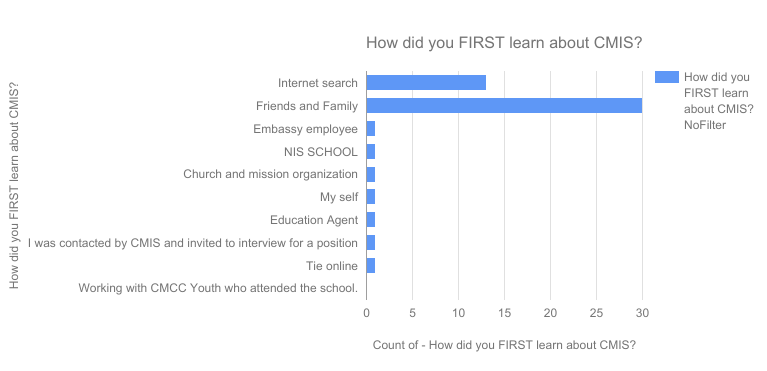
\includegraphics[width=\textwidth]{profile37}
\caption{How did you FIRST learn about CMIS?}
\end{figure}

Results of the New Family Survey show that most of our new families learn about CMIS from word-of-mouth, followed by Internet search. Knowing this has enabled us to focus our attention on these two areas of publicizing the school. In the 2016-17 academic year a new version of the school website was launched. Emphasis was put on highlighting the best parts of CMIS and making it easy for new families to find information about admission, enrollment, and student life.

\begin{figure}
\centering
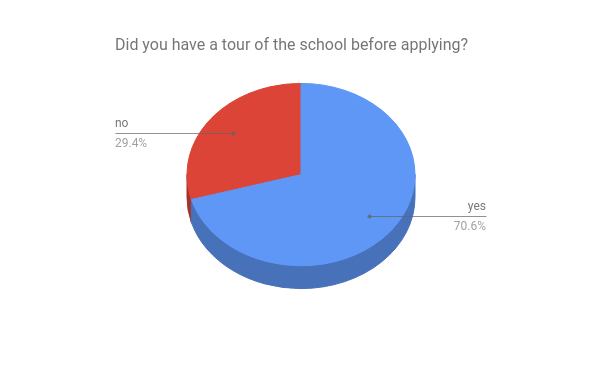
\includegraphics[width=\textwidth]{profile38}
\caption{Tour Survey Question 1}
\end{figure}

\begin{figure}
\centering
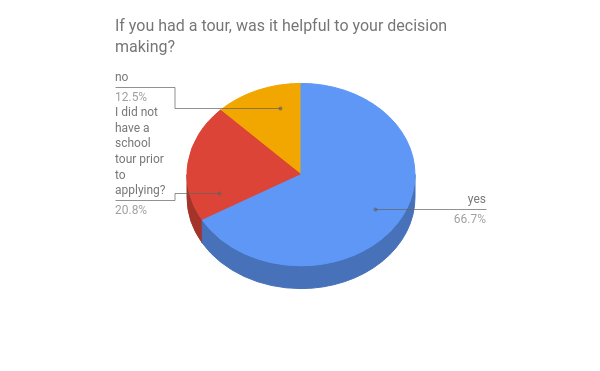
\includegraphics[width=\textwidth]{profile39}
\caption{Tour Survey Questions 2}
\end{figure}

\begin{figure}
\centering
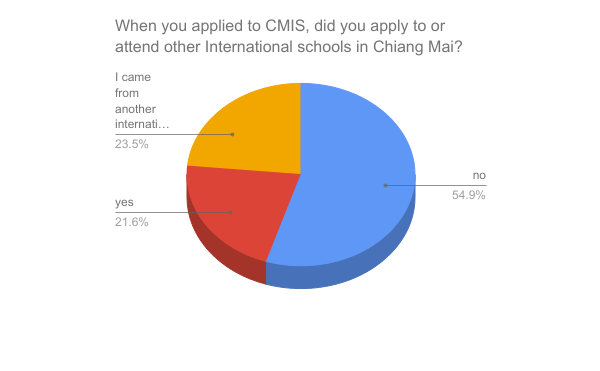
\includegraphics[width=\textwidth]{profile40}
\caption{Tour Survey Question 3}
\end{figure}

We also learned that most respondents had a school tour prior to applying, 70\%, and that the school tour was helpful in making the decision, 66\%. Additionally families surveyed did not apply to other international schools in Chiang Mai, indicating CMIS as their school of choice.

Of the reasons Families choose CMIS, Teachers, Community, and Curriculum were the most prevalent followed by the diversity of the student population, facilities, and location. Tuition was not indicated as a factor in deciding to come to CMIS.

\tcbsection{Conclusion}

Since our last WASC report in 2011, CMIS has gone through a period of growth and development, while remaining true to its mission and vision. Enrollment and staffing have increased incrementally, and a plan has been implemented to develop the facilities accordingly. Our Board and school leadership teams have held firmly to our school mission and vision by developing and refining our Student Learner Outcomes. 

Increased demand for enrollment has presented us with opportunities to maximize student diversity and apply higher standards for entry. We maintain a diverse student population, and select qualified, priority applicants for enrollment before considering all others on a space-available basis. We also place limits on our population's demographics in order to maintain the school's English-speaking environment and diverse, international character. 
 
Application to CMIS is competitive, and managed through an online application system. Newly selected students are surveyed to help identify areas in which we need to improve our processes and focus our advertising. The respective roles of the school website and the admissions tour have been identified as important factors affecting our applicants' decision to apply to CMIS. 

All students have to demonstrate English-language proficiency and qualify academically for their grade level before they can be considered for enrollment. Students are also required to meet the behavioral, emotional, and social expectations of the CMIS student body. Applicants are selected by an Admissions Committee, who also considers the available resources and existing student population when selecting new students.  

The quality of our teaching staff ranks highly among the reasons why people choose to study at CMIS. Our teachers are highly qualified, and our school's administrative structure is effective for efficient operation and management. CMIS has demonstrated its commitment to obtaining and retaining quality teaching staff by providing increased opportunities for Professional Development (PD). Since the time of our last WASC report, monthly scheduled PD time as well as a designated fund for professional development has been established and utilized to effectively support student learning through teacher training.

Our teachers and administrators are satisfied with the working conditions at CMIS, and often stay for multiple 2-year contract periods. The diversity of our teaching staff provides a stimulating environment in which our cultural differences are celebrated and respected. We currently have staff from 15 different countries. All staff are required to be fully certified and have at least a Bachelor's degree in their respective areas of expertise. Over a third of our staff possess advanced degrees.

College planning is an integral part of our CMIS high school program. Our students are given guidance and assistance in planning their applications for admission to colleges and universities around the world. In general, all of our graduating seniors are matriculated into the programs of their choice, with some choosing to take a gap year to perform community service before beginning their post-secondary studies. 

Opinion surveys have been used to solicit feedback from students, staff, and members of our CMIS community. Responses to surveys have helped guide our school administrators in targeting improvements for each respective group. Whenever areas of concern have been identified, actions have been taken to address the situation and progress has been communicated to the affected community. School administrators have continued to encourage communication through various venues, including staff meetings, student communication groups, monthly PTG meetings, and the Teacher/Administration Communication Team (TACT). 

An emphasis on research-based management led to the realization that limited data was available on CMIS Student Learner Outcomes. The Datawise initiative was taken in response to the need for qualitative data on student performance. Steps were taken to understand the available DRAs, PSAT and SAT scores, AP test results, and ISA test results in light of the CMIS Common Core Objectives. To the extent possible, this data was used to identify student needs and create action plans for improvement. In addition, CMIS has adopted the NWEA MAP (Measures of Academic Progress) school wide in order to produce more useful data that can be used to support modifying student instruction.  

CMIS places high importance on providing opportunities for Student Life Beyond the Classroom. Much has been done to identify and address items of concern to our CMIS community. We will continue the process of annually refining and conducting perception surveys. As a school, we regularly celebrate the progress we are making and make concerted efforts to share this information throughout the CMIS community. 

We are blessed with an intelligent, talented, caring, group of highly qualified staff. Our administrative structure is supportive of staff and schoolwide initiatives. Leadership is effective in implementing change and responding to the needs of our community. The result has been a greater focus on student learning and closer adherence to our school mission and vision. 

The process of looking at data has identified the need for additional data, especially with respect to student learning and performance, and the need for a central data repository. The school will continue to involve all stakeholders in the improvement process, knowing that a collaborative, consultative approach to planning and implementation is the most effective means to bring about and sustain positive, long-lasting change that promotes student learning. 


\tcbchapter{Progress Report}
\AddToShipoutPicture*{\BackgroundPic{chapter2.jpg}}

\section{CMIS RESPONSE TO RECOMMENDATIONS FROM PREVIOUS REPORT }
\subsection{Item 1}

\minor{Action Plan}

Continued development of the written, taught and assessed curriculum at all levels, with the goal of a comprehensive curriculum document that includes standards and benchmarks, assessment tools, resources, technology integration and sample units for all subject areas and grade levels. This would be evaluated at all levels to check for coverage and continuity, as well as to ensure that Educational Objectives were being thoroughly covered in our program. It would also include a regular evaluation and improvement system being put in place and maintained.

\begin{longtabu} to \textwidth {|X|X|}
\hline
\textbf{Growth Area 2011} & \textbf{Steps Taken Since Interim Report 2014} \\
\hline
1. \minor{Curriculum} EOs (ESLRs): Reflect on the appropriateness of the Educational
Objectives, develop processes for alignment and integration into the curriculum, instruction and school activities, and create appropriate measurements for student mastery. &

\parbox[t]{2.8in}{
Modify EOs (ESLRs) to SLOs\\
Staff involvement in SLOs creation \\
Modification of EOs into measurable SLOs\\
Integration of SLOs with UbD units\\
Instructional Round data collection of SLOs applications \\
Implementation of SLOs into student communication group activities\\
Student created visuals of SLOs }\\
\hline

2. \minor{Curriculum} curriculum development and documentation - Continued development of a standards based, comprehensive, progressive, written curriculum in elementary social studies, science, and non-core courses in the arts, as well as continued development of secondary courses to ensure a CMIS curriculum (including curriculum maps) are in place and is sustainable; and develop a schedule for regular assessment and revision of curriculum through a curriculum renewal cycle and process. &

\parbox[t]{2.8in}{
Unpacking of CCSS ELA, CCSS Math, NGSS, and C3\\
Training on Understanding by Design (whole group, small group)\\
Implementation of UbD Unit Menu\\
Modification and use of UbD template to reflect current professional practice\\
Development and use of Adoption/Resource Cycle \\
Development and use of research based adoption vetting instruments\\
Development and use of Scope and Sequence Blueprints K-12\\
Collection of best practices in Summative Assessment development \\
Development for and implementation of Datawise process \\
Use of Instructional Rounds observational process\\
Use of Teach for Success observation protocol\\
Implementation and training of staff for Datawise data analysis process\\
Training of staff for Middle School ELA/SS Alignments and PARCC Blueprints\\
Training of staff for High School ELA PARCC Blueprints\\
Development and implementation of UbD Interrater Reliability Practicum} \\
\hline

3. \minor{Curriculum} instruction and assessment - Utilize current and research-based instructional strategies systematically and with the support from the leadership. Implement a schedule for reviewing  assessment practices (formative and summative) and results to inform curricular and instructional decisions; and implement grade level common assessments (standardized or otherwise) for levels that currently do not have them. &

\parbox[t]{2.8in}{
Development and implementation of Formative Assessment training\\
Development and implementation of Summative Assessment Peer Reflection (for HS only)\\
Modification and use of UbD template to reflect current professional practice in formative and summative assessment\\
Modification and use of UbD template to reflect current professional practice in literacy and rigor (e.g. close reading, DOK)\\
Development and implementation of school wide writing pre assessment \\
Development and implementation of common ELA writing rubric for argumentative writing\\
Development and implementation of Looking at Student Work protocols (e.g. Critical Friends, Longfellow Slice)\\
Implementation of MAP Assessment for grades 2-9 \\
}
\\
\hline
\end{longtabu}

\subsection{Item 2}

Develop a process of continuously evaluating and prioritizing foreign teacher
compensation and benefits to encourage them to extend their stay in CMIS. This may also include evaluating teacher workloads, schedules, recognition opportunities and extra responsibilities including substituting. This will include forms of evaluation and follow-up and a system for staff and teacher evaluation that is comprehensive and transparent. In addition, effective procedures for due process, renewal of contracts, and grievances will be developed.

\begin{longtabu} to \textwidth {|X|X|}
\hline
\textbf{Growth Area 2011} & \textbf{Steps Taken Since Interim Report 2014} \\
\hline
4. \minor{Professional Development} Further implement the professional development plan so professional development is focused on prioritized and definable school curricular needs as seen in Growth Areas 1-3. Professional development needs to purposeful and sustained to improve student learning.
 &

\parbox[t]{2.8in}{
Unpacking of CCSS ELA, CCSS Math, NGSS, and C3\\
Development and delivery of training on Key Instructional Shifts in ELA\\
Development and delivery of training on Key Design Elements in CCSS\\
Development and delivery of training on Formative Assessment\\
Development of Summative Assessment Peer Reflection \\
Development and delivery of  training on Text Complexity\\
Training on UbD Essentials (outside consultant)\\
Development and delivery of training on Building Knowledge Systematically in CCSS\\
Development and delivery of training on Close Reading \\
Development and delivery of training on Student Engagement Essentials \\
Development and delivery of training on Text Dependent Questions\\
Development and delivery of training on Tier 2 and 3 Vocabulary development\\
Development and delivery of New Teacher Orientation modules\\
Development and delivery of training on SMART goals\\
Development and delivery of training on NGSS through use of vetting instruments\\
Development and delivery of training on CCSS  Mathematics through use of vetting instruments\\
Development and delivery of training on C3 unpacking, Scope/Sequence, and Unit Creation using IDM  }\\
\hline

Teacher compensation and evaluation: Further refine and implement a process of continuously evaluating and prioritizing foreign teacher compensation and benefits to encourage them to extend their stay at CMIS. This may also include evaluating teacher workloads, schedules, recognition opportunities and extra responsibilities, including substituting. This will include forms of evaluation and follow-up and a system for staff and teacher evaluation that is comprehensive and transparent. In addition, effective procedures for due process and renewal of contracts and grievances must be developed.
 &

\parbox[t]{2.8in}{
Increase staff salary step and housing benefit\\
Creation of staff attendance incentive\\
Creation of Teacher Leadership Team\\
Increase in Teacher Leadership stipend\\
Creation of stipends for staff coaches \\
Creation of professional development fund for all staff\\
Creation of new Staff Welcome Committee\\
Creation of New Hire Buddy Program\\
Creation of New staff handbook \\
Creation of New staff orientation \\
Creation of Free Certified First Aid Training for volunteer foreign staff\\
Workload analysis data and workload payment committee\\
Scheduling modification to increase staff collaboration time\\
Creation of Staff Grievance Policy (formal and informal)\\
Annual TACT meeting for salary and benefit every 2 years\\
Creation of Monthly Kudos Cup (staff appreciation)\\
Creation of specific timeline for renewal of contracts ( end Jan.)\\
Creation of simplified contract template for 2017-18\\
Creation of exit interview for leaving staff\\
Creation of Substitute coordinator position on campus\\
Extra pay for staff using preparation time for substitution\\
Use of Instructional Rounds observational process\\
Use of Teach for Success observation protocol\\
Implementation and use of The Essential Practices of High Quality Teaching and Learning\\
Development and delivery of training on Depth of Knowledge } \\
\hline
\end{longtabu}

\subsection{Item 3}

Develop administrative and Board policies and procedures that are well documented, clearly communicated and effective for the daily running of the school in regards to the school board, principals, business manager, and director.

\begin{longtabu} to \textwidth {|X|X|}
\hline
\textbf{Growth Area 2011} & \textbf{Steps Taken Since Interim Report 2014} \\
\hline
5. \minor{Board} policies and procedures - Develop School and Board policies and procedures that are well documented, clearly communicated and effective for the daily running of the school in regard to the Board, principals, business manager, and director. Furthermore, policies and decision-making processes must be visible and transparent to all stakeholders.
 &

\parbox[t]{2.8in}{
Creating a specific CMIS Board Handbook, \\
Creation of Board policies: Principles of Good Practice and Individual Board Member Principles of Good Practice \\
Modification of Faculty Handbook format\\
Updated policies and procedures reviewed annually at staff orientations \\
Implementation of Wednesday staff meetings\\
Creation of Board meeting summaries available to community\\
Implementation of Parent Coffee Mornings at start of the school year\\
CMIS Board/SET members attend monthly PTG Meetings\\
Board/SET members are involved with the New Teacher Orientation day\\
Board/SET members participate in FOL/WASC focus groups \\
Board generates annual community letters  }\\
\hline

6. Board training: To help ensure sound governance, the board should develop a process for consistent board training and orientation as well as board self-evaluation.
 &

\parbox[t]{2.8in}{
Creation of Board retreats for training, orientation and self-evaluation. \\
Utilization of outside consultant John Ritter worked with Board \\
CMIS membership National Association of Independent Schools \\
Creating new Board member mentorship and training } \\
\hline
\end{longtabu}

\subsection{Item 4}

Create a school wide master plan which will include planning for the development of new or existing property, a budget and resource acquisition system that aids educational planning for departments, IT equipment, books, materials, other resources, and capital improvements.

\begin{longtabu} to \textwidth {|X|X|}
\hline
\textbf{Growth Area 2011} & \textbf{Steps Taken Since Interim Report 2014} \\
\hline
8. \minor{Resources, facility, master plan} Further develop a school-wide master plan that includes planning for the development of new or existing property, a budget and resource acquisition system that aids educational planning for departments, IT equipment, books, materials, other resources, and capital improvements. The plan should include involvement of all stakeholders to help ensure the planning process is transparent.
 &

\parbox[t]{2.8in}{
Creation of Campus Development Plan\\
Analysis of community survey plan\\
Development and implementation of 10 year Adoption/Resource Cycle. \\
Development and implementation of Resource Request and Resource Renewal procedures and forms \\
Development and implementation of vetting and evaluation instruments for resource adoption   }\\
\hline

\end{longtabu}

\subsection{Item 5}

 Continue to improve and expand communication among all stakeholders at CMIS.

\begin{longtabu} to \textwidth {|X|X|}
\hline
\textbf{Growth Area 2011} & \textbf{Steps Taken Since Interim Report 2014} \\
\hline
9. \minor{Communication} CMIS needs an effective communication system to inform all stakeholders of school processes and procedures, decision-making responsibilities, and school-wide issues, and information including student progress.
 &

\parbox[t]{2.8in}{
Increase in Facebook/social media community communication\\
Creation of Administration Parent newsletter\\
Implementation of Emergency messages through SMS\\
Implementation of Power School communication alerts\\
Greater use of Google Classroom and guardian access to Google Classroom \\
New formated website with greater emphasis on finding information and weekly communication. 
Weekly faculty notes  }\\
\hline

\end{longtabu}

\subsection{Item 6}

Expand our community connections to include an alumni association and development office to increase opportunities to raise support from places other than just tuition.

\begin{longtabu} to \textwidth {|X|X|}
\hline
\textbf{Growth Area 2011} & \textbf{Steps Taken Since Interim Report 2014} \\
\hline
NA
 &

\parbox[t]{2.8in}{
Creating a fund development committee to increase communication,\\
facilitate volunteer involvement, and encourage philanthropic commitment to CMIS.\\
Utilizing an alumni coordinator to develop and maintain an effective alumni database. }\\
\hline

\end{longtabu}



\tcbchapter{Student/Community Profile: Overall Summary from Analysis of Profile Data and Progress}
\AddToShipoutPicture*{\BackgroundPic{chapter3.jpg}}
\tcbsection{What are the implications of the profile and progress data with respect to student performance since the prior self-study (or initial visit)?}

\minor{Notices from profile data since last self-study:}
\begin{itemize}
\item Increase in student population from 459 to 506
\item Developed a viable, actionable Campus Development Plan
\item Demographics have changed resulting in 3% increase in non-native English speakers
\item Assessments used previously are no longer valid as adopted standards have changed
\item In terms of tuition, the discount category has decreased while the standard category has increased thus providing more income for school growth.
\item Almost all CMIS graduates matriculate to postsecondary education. 
\item Schoolwide learner outcomes were updated to reflect measurability and global citizenship
\end{itemize}

\minor{Student Learner Outcomes}
Courageous Learners who: 
\begin{itemize}
\item Embody a work ethic that values learning and academic integrity
\item Pursue personal growth as adaptive, independent learners
\item Exhibit thinking that is open minded, creative, and takes risks
\item Utilize resources and technology to effectively support learning and work
\end{itemize}

Responsible Global Citizens who:
\begin{itemize}
\item Understand Christian virtues and positive student character 
\item Demonstrate integrity through consistent respect for people of all faiths
\item Develop cultural awareness and an appreciation for diversity
\item Serve as responsible, proactive members of the global community
\end{itemize}

Recognizing the need to instill citizenship and the CMIS core virtues, the school has taken steps to coordinate and promote our community values.  In the elementary program, our school counselor teaches weekly interactive virtues lessons to each grade level.  In addition the counselor, principal, teachers, and students facilitate a monthly Virtues Assembly that highlights a different virtue each month. These events are well attended by our community.

In order to instill a philosophy of giving to to those in need, the middle school students visit a local orphanage once each semester.  The students work with the volunteers and children by organizing activities and events to develop a sense community and global advocacy.  This fall, CMIS used the annual Harvest Festival as an opportunity to collect donated goods for Hope House, a local orphanage supported by members of the school community.  Every other Tuesday, middle school students pair with an elementary student to read a book aloud to them in the CMIS Reading Buddies program.  This enables our older students to serve as models to younger students.  

The entire school community has participated in the global initiatives, “Mix it up at Lunch Day” developed by Teaching Tolerance foundation and “Great Kindness Challenge”, organized by the Kids for Peace organization, to promote our school vision as place that respects and celebrates diversity. The “Mix it up at Lunch Day” encourages students to sit and interact with students that they may not know well. This is a simple act with profound implications. Studies have shown that interactions across group lines can help reduce cultural misunderstandings. When students interact with those who are different from them, biases and misperceptions can fall away.  The “Great Kindness Challenge”, encourages students to perform virtuous acts of kindness to students and adults on campus. In addition, middle school and high school students are assigned to communication groups, in which their teachers provide some level of individualized pastoral care.  

{\centering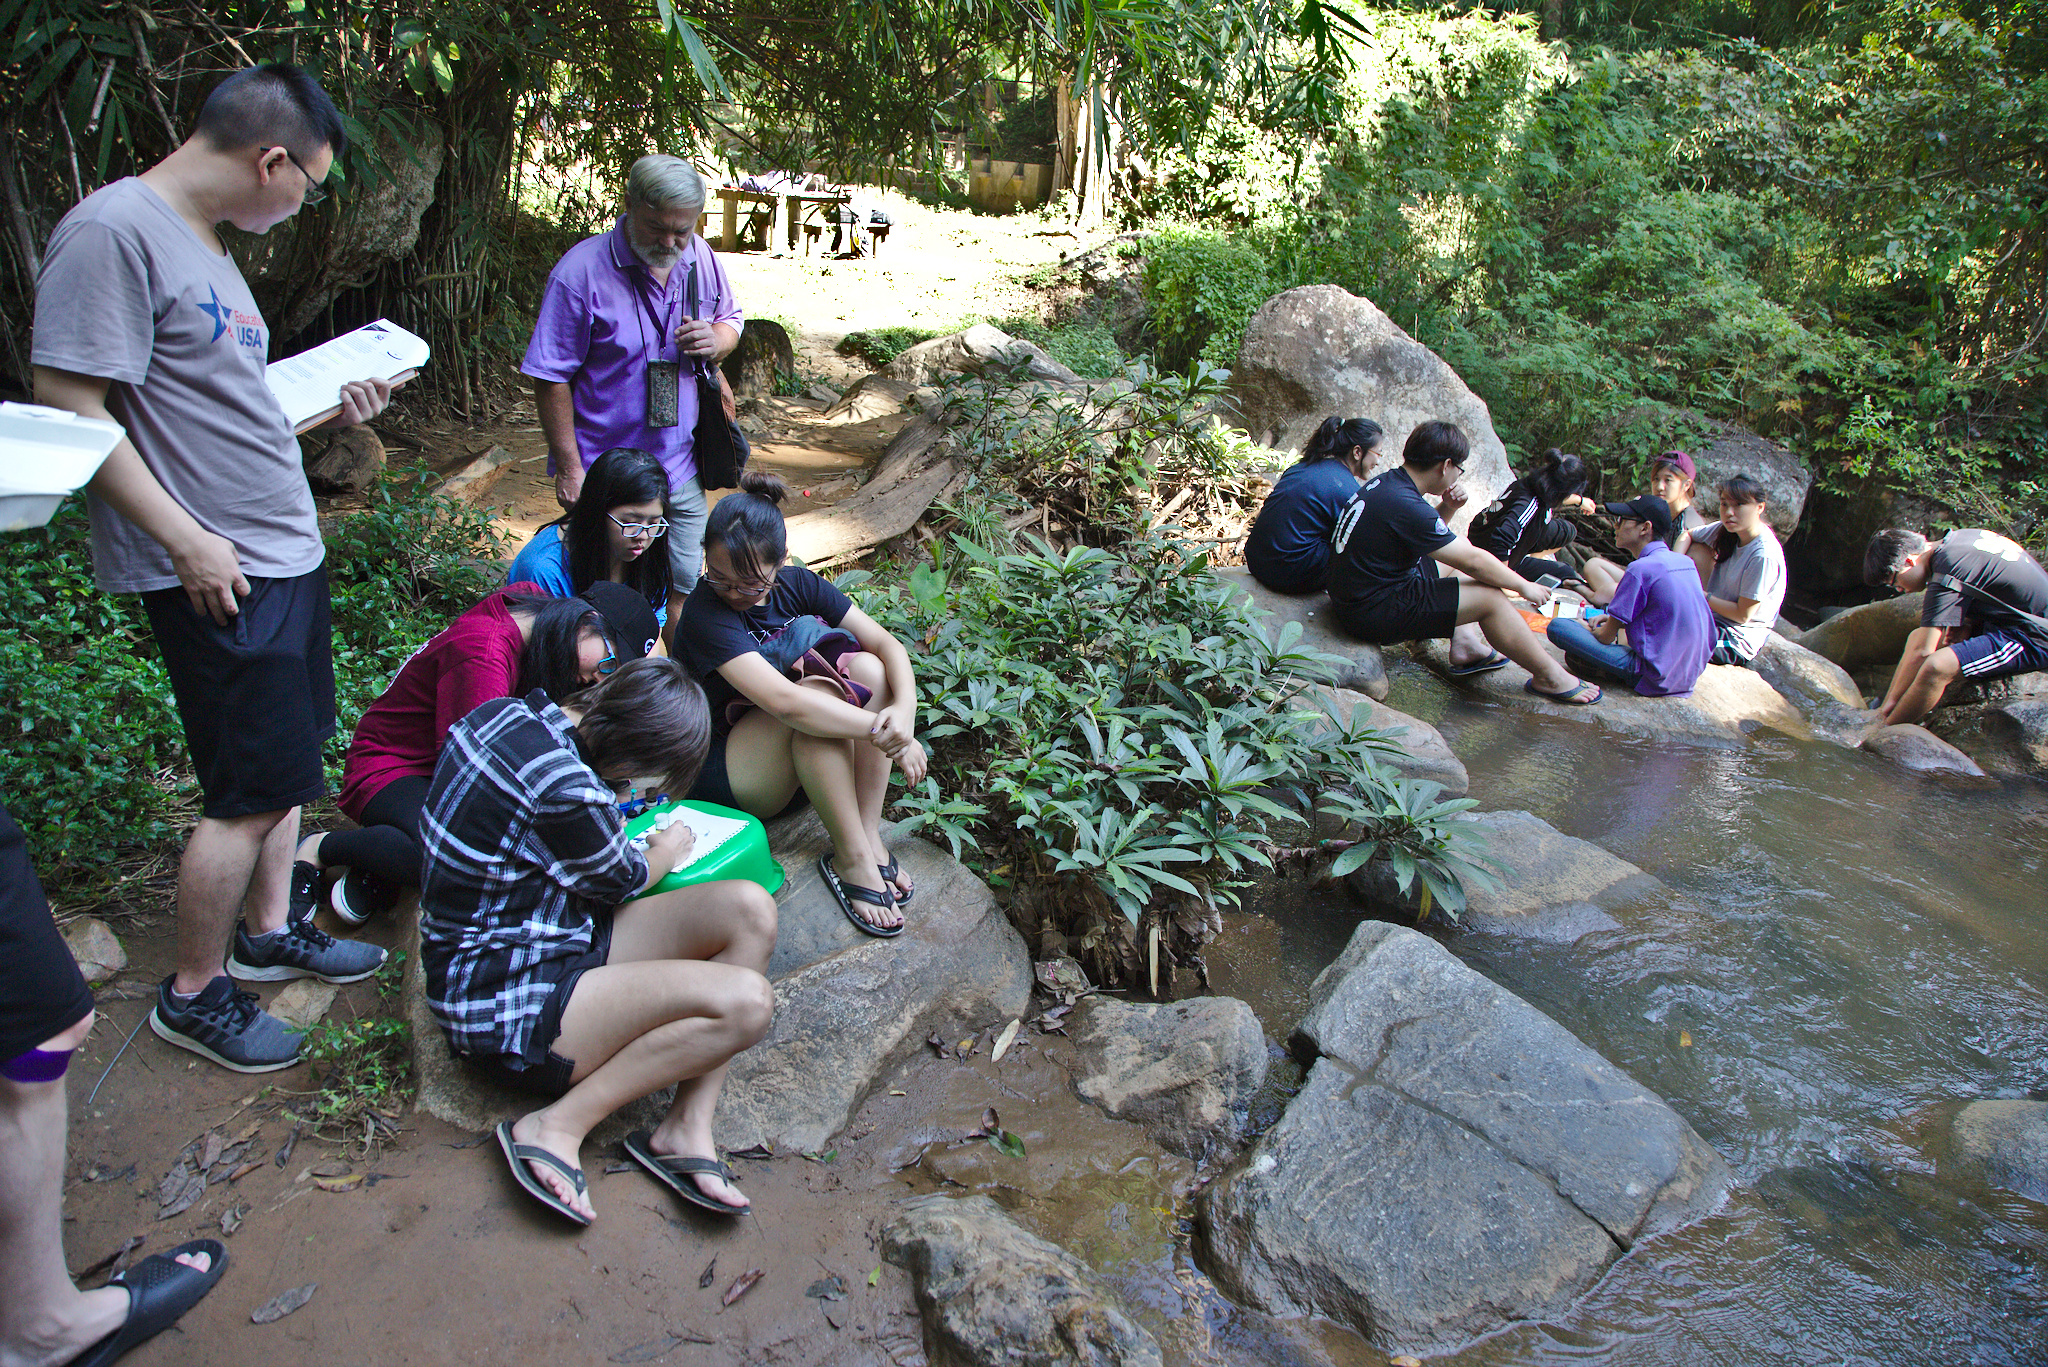
\includegraphics[width=\textwidth]{chapter3science_fieldtrip.jpg}}

High school students learn to take ownership of the schoolwide learner outcomes by participating in community service activities. The CMIS Community Service Coordinator has encouraged students to create their own community service projects that align with our schoolwide learner outcomes. This transfer of responsibility encourages student inspired community advocacy.  CMIS Leadership also encourages group community service projects that build student collaboration and group accountability. By earning community service credits, high school students demonstrate proactivity in planning and implementing their own projects.  Community service projects for high school students are also encouraged within the CMIS community, such as: 
\begin{itemize}
\item Reading Buddies to elementary students, which supports school cohesiveness (and student reading comprehension). 
\item Homework Club to middle and elementary students, which promotes student achievement in a caring environment. 
\item Parent facilitators, such as English translators, campus orientation guides, and childcare assistants during family conferences, which increases parent participation and develops student responsibility.
\end{itemize}

CMIS has sought to uphold the rich Christian heritage upon which it was founded while continuing to welcome those of differing religious backgrounds, cultures, and beliefs. Within this spirit, CMIS has encouraged students to learn about God’s love and the Christian faith so they can make their own personal and intelligent response to it. The all school Christmas and Easter assemblies, various prayer meetings, and weekly faith-based clubs have been designed with this purpose in mind. Each week, there are several different opportunities for students to be involved in learning more about the Christian faith if they desire. CMIS has a Student Spiritual Advisor to facilitate these faith based programs and to serve as a positive role model and advocate for all students.

CMIS has also modified the policies and procedures in the Student Planner/Handbook to emphasize research based best practices. Rather than focusing on repercussions of negative behaviors, the emphasis is on positive behaviors that create responsible and proactive members of the global community.  For example, addressing student digital citizenship, students practice how to respect intellectual property rights and to avoid plagiarism through engaging lessons and activities, rather than reviewing a list of consequences. 

Since the self-study, CMIS has taken steps to regularly analyze data. We adopted the Datawise process to help teachers through the process of analyzing student performance data. Teachers also regularly peer review assessments using a common peer review form. The CMIS Leadership has begun to create a culture of looking at data and will continue to use data to modify instruction in respect to student performance. CMIS Leadership Team also understands the need to create a online, data “sandbox” where we can access multiple forms data to help teachers analyze student performance and make instructional adjustments to address our learner needs.

CMIS has made significant improvements in both the resource adoption, request, and renewal process. Since CMIS adopted new standards in 2013, updated, aligned, rigorous, and engaging resources have been vetted, evaluated, and adopted in science and mathematics. All teachers are involved in the vetting, evaluation, and selection of adopted resources. All adoption meetings involved targeted professional development on the standards, rigor, and instructional shifts. 

In 2014-2015, CMIS began a development program to familiarize teachers with the CCSS Literacy standards and to create blueprints of unit studies and lesson plans using the Understanding by Design (UbD) approach. More time is required to fully implement these standards throughout their UbD units. Teachers worked in departments to create these blueprints and lesson plans with oversight from our Curriculum Director.  

\tcbsection{Based on past performance and current data, select two to three critical learner needs, noting the correlated schoolwide learner outcomes.}

Based on our reported percentage of students from an English-speaking background, CMIS is categorized differently by ISA each year. Thus, a year-by-year comparison with like schools is hard to make and interpret. Because of the challenge, the CMIS Teaching Staff have used the Datawise process since 2014, in which a study of the ISA data identified the need for students to further develop their expository/argumentative writing skills.  A school-wide writing assessment was given to further confirm this need, and an action plan was created to scaffold the students that needed extra attention with this particular skill. CMIS also used this opportunity to create a common assessment rubric for English Language Arts (ELA) and Social Studies departments. In 2015 the Datawise process indicated a need for student improvement in writing organization. Teachers researched and adopted department graphic organizers as a common intervention strategy. In 2016 the Datawise process indicated that student progress was difficult to evaluate as teachers within the same department were incorporating different assessment techniques and formats. It also highlighted the need for consistent, standards based, school-wide student data. As a result, teachers are currently working on the creation of consistent assessments and the school will be implementing the comprehensive assessment platform, Measure of Academic Progress (MAP), which is a standards-based assessment that can be implemented school-wide.

Based on the data we have found, while a majority of our students perform well on standardized tests (PSAT 8/9, SAT/NMSQT, SAT), some students are not reaching the College Board benchmarks. To correlate this with student performance in class, we need to provide teachers with timely PSAT data to determine the extent to which low PSAT performances are related to testing anxiety versus gaps in learning. Adding the MAP test will also add more data to help teachers identify skill deficits and modify instruction to meet student needs. Additionally, CMIS has included Grades 8 and 9 in PSAT testing in 2015-2016 to proactively address test anxiety and to give students an opportunity to practice SAT testing. 

\minor{Correlated SLOs}

Pursue personal growth as adaptive, independent learners, exhibit thinking that is open minded, creative, and takes risks, and utilizes resources and technology to effectively support learning and work.

\tcbsection{List 3-4 important questions that have been raised by the analysis of the student performance, demographic, and perception data and the progress data.  (These will be used in the Home and Focus Group work.)}

\minor{Question 1: How do our assessments align with the rigor of the standards?}

This question was given to teachers as they peer reviewed their assessments and evaluated student work samples. The purpose was to ensure that teachers were implementing the standards to the correct alignment and rigor as stated in the standard. This is a continuing discussion in department and divisional meetings.

\minor{Question 2: How did formative assessment inform one of your decisions today or this week with a student, a subset of students, or a class?}

This question was used to have teachers discuss the purpose of and the effective use of formative assessments in their classes. As formative assessment has played a central role in CMIS professional development for the past two years, CMIS Teaching staff have begun to reflect on this question with greater frequency. 

\minor{Question 3: How are we supporting students who have not demonstrated proficiency? }

This question was specifically used to analyze the way in which we identify struggling learners. It was also used to identify and remind teachers of the Student Support Team and how it is a resource for students’ academic, emotional, and social achievement.

\minor{Question 4: How can MAP and other standardized testing data be used to inform decisions?}

This question was used to overview the purpose of the MAP assessment. It encouraged teachers to identify the possible ways that large scale standardized testing can provide additional insight into their instruction. 

\minor{Question 5: How can we maintain our current student diversity in a growing international school market?}

This question was asked within the admission and leadership teams. It is an ongoing conversation that reflects upon the demographics of the Chiang Mai community and the increasing competition with local international schools. 


\tcbchapter{Self-Study Findings}
\AddToShipoutPicture*{\BackgroundPic{chapter4.jpg}}
%% ORGANIZATION FOR STUDENT LEARNING
\tcbsection{Organization for Student Learning}
\subsection{A1 School Purpose Criterion}
\subsubsection{Beliefs and Philosophy}

\indicator{The written mission and vision reflects the beliefs and philosophy of the school and its constituency.}

\prompt{Evaluate the written purpose in relationship to the beliefs and philosophy of the school and its constituency served.}

\begin{findings}
CMIS has a clear Vision, Mission and Student Learner Outcomes that reflect the beliefs and philosophy of the school. These are widely published and easily visible to the community. \href{http://cmis.ac.th/about/vision}{CMIS Vision and Mission}
 
{\centering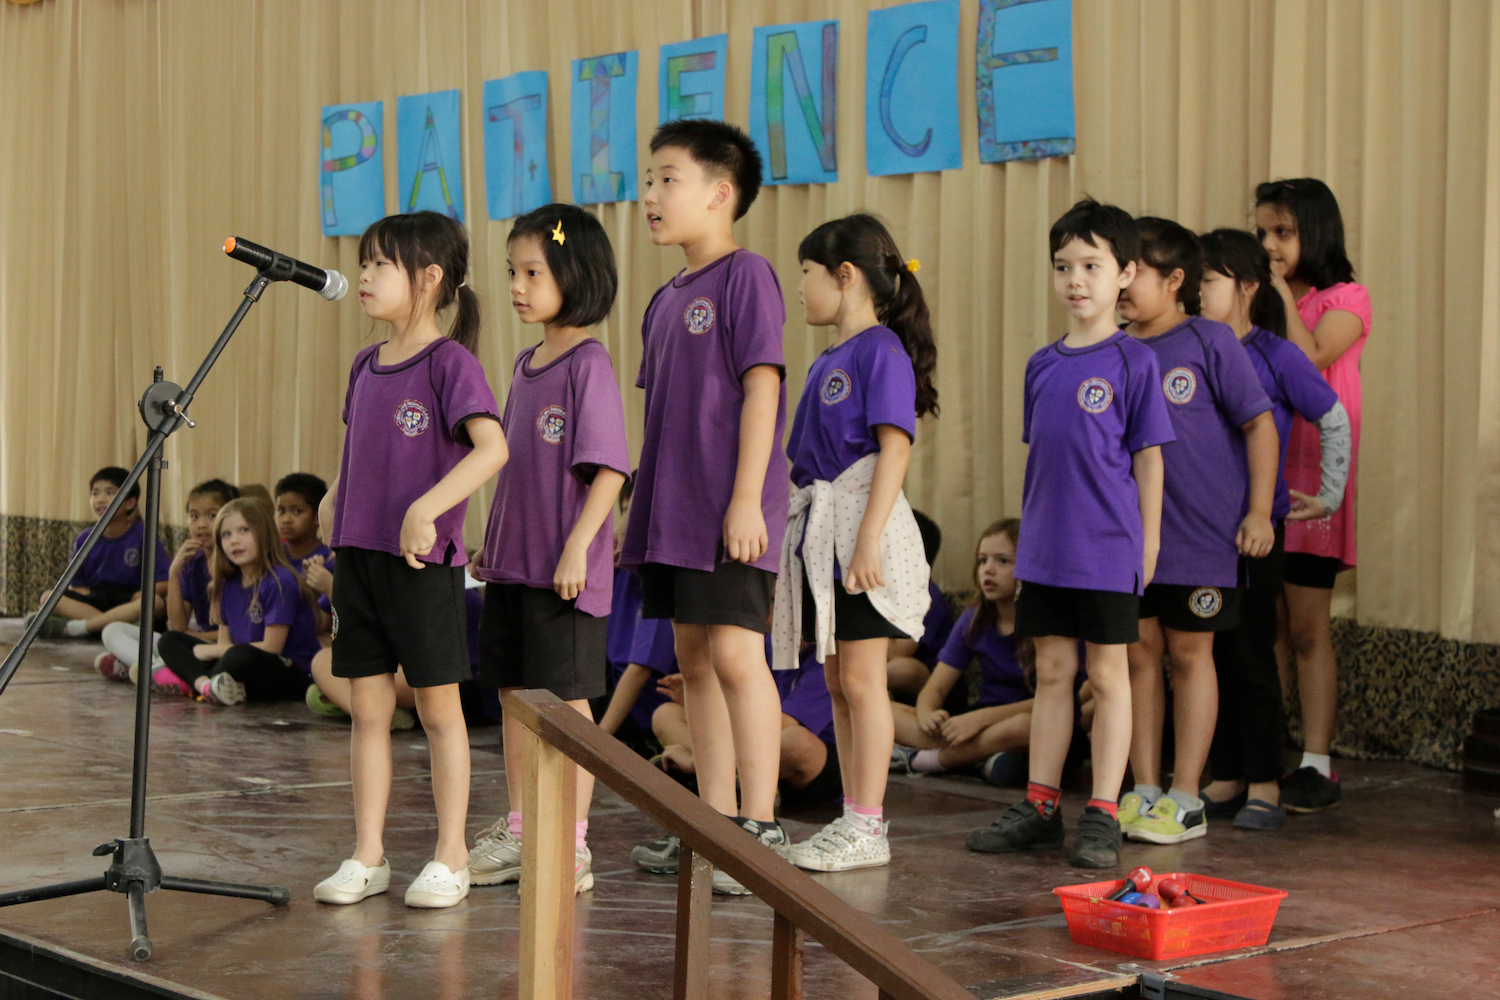
\includegraphics[width=\textwidth]{4_1_1_b.jpg}}

CMIS stakeholders strive to continuously uphold the mission of providing educational excellence, in a caring Christian community that celebrates and respects diversity. \href{https://docs.google.com/a/cmis.ac.th/presentation/d/1EJ3zT-xwUj2W--v5mTN6xWOqewtvhXrhTxXuoR1HyAg/edit?usp=sharing}{CMIS Mission Statement Project} 

The current version of our mission statement resulted from the work of a committee of board members, administrators, teachers, and parents in 2014-2015. Though recently updated, the CMIS mission is still aligned to the historical values of the school.

This year, our student learner outcomes posters displayed around campus were designed and created by our grade 6-12 students. Who We Are Student Poster Competition 

\minor{So what...}

CMIS has a clear Vision, Mission and Student Learner Outcomes that reflect the overall goal of the school community. These are continuously referred to and well known throughout the community. 

We need to find more opportunities to receive feedback from parents on the relevancy of our school “purpose” so we can remain confident that it reflects the beliefs and philosophy of the whole school and its constituency.
\end{findings}

\subsubsection{Purpose, Schoolwide Learner Outcomes, and Profile Data}

\indicator{The student/community profile data and identified global competencies have impacted the development of the school’s vision, mission, and schoolwide learner outcomes.}

\prompt{Evaluate the degree to which the development of the school’s vision, mission, and schoolwide learner outcomes have been impacted by pertinent student/community profile data and identified global competencies, and current educational research}

\begin{findings}
Our community profile data has greatly impacted the development of the\href{http://cmis.ac.th/about/vision}{ CMIS’ Mission, Vision and Student Learning Outcomes Statement}:

{\centering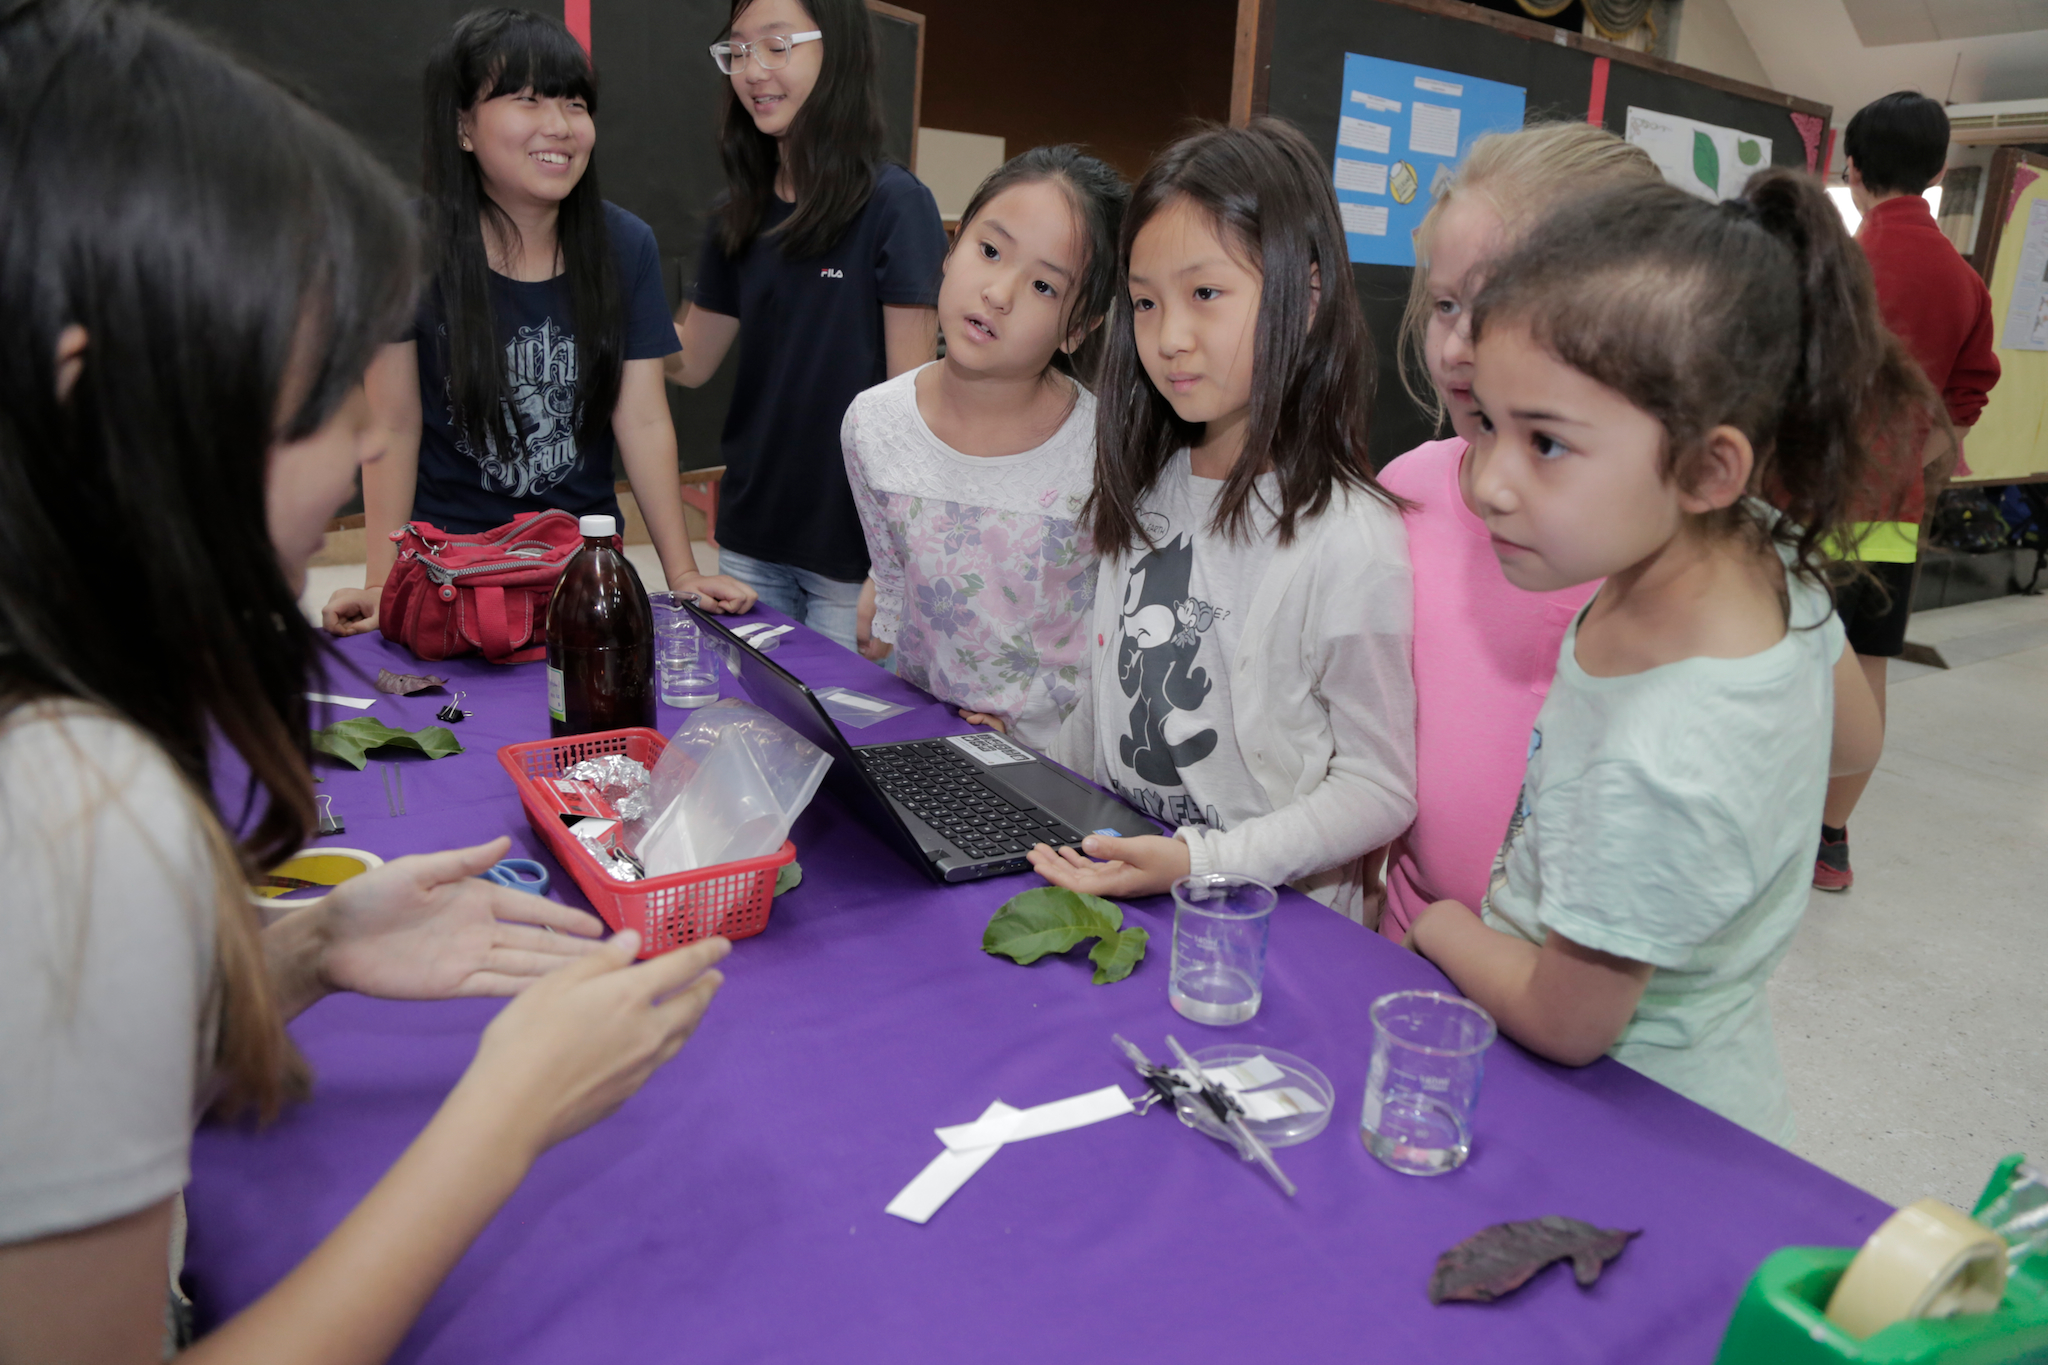
\includegraphics[width=\textwidth]{4_1_1_c.jpg}}

Our \href{https://docs.google.com/document/d/1bIbV9pgGz2vpXYJdnRzL_Od5PS35egy7lgBOBuszgD4/edit}{Student Learner Outcomes} (SLOs) were modified from their original format as Educational Objectives in 2015 to better recognize our diverse student population (32 different nationalities), embrace our global citizenship responsibilities, and include updated 21st century skills. These outcomes were reviewed with all students at the beginning of the 2016-2017 school year and their interpretations were displayed as posters across campus. \href{https://docs.google.com/a/cmis.ac.th/presentation/d/1bdi1LZUjWbGKOyB0XR9CGyoY2xLY39SZVKhiHTIJGxc/edit?usp=sharing}{Student Poster Competition}.

Our diverse group of \href{http://www.cmis.ac.th/about/faculty}{highly qualified educators} originating from over 12 different countries reflect the different cultures and nationalities of our community. Our additional support staff positions also reflect our efforts to meet our community needs (examples: Korean liaison and student spiritual advisor).

CMIS addresses global competencies in a variety of ways beyond the school mission and SLOs. Academically, CMIS students are engaged in learning standards that are internationally benchmarked and rigorous. \href{https://drive.google.com/drive/folders/0ByVFfrm0zfolMVRQYmI1aGlRNDQ}{CMIS Teaching Standards K-12}.

CMIS students have multiple opportunities to engage in school activities and events that require global understanding (e.g. \href{http://gallery.cmis.ac.th/zp-core/full-image.php?a=2010-2011/thai-day-2011/website&i=_mg_3802-version-2.jpg&q=100&wmk=\%21&dsp=Protected\%20view&check=788a1e55c231186711f8dcc0876f4efd0daa0880}{Thai Day}) celebration of diversity (\href{http://gallery.cmis.ac.th/zp-core/full-image.php?a=2013-2014/international_day&i=_MG_6129.jpg&q=100&wmk=\%21&dsp=Protected\%20view&check=788a1e55c231186711f8dcc0876f4efd0daa0880}{International Day}) sharing multiple perspectives (e.g. \href{https://www.nhd.org/}{National History Day}) and using multilingual skills (e.g. Model United Nations Club). 

{\centering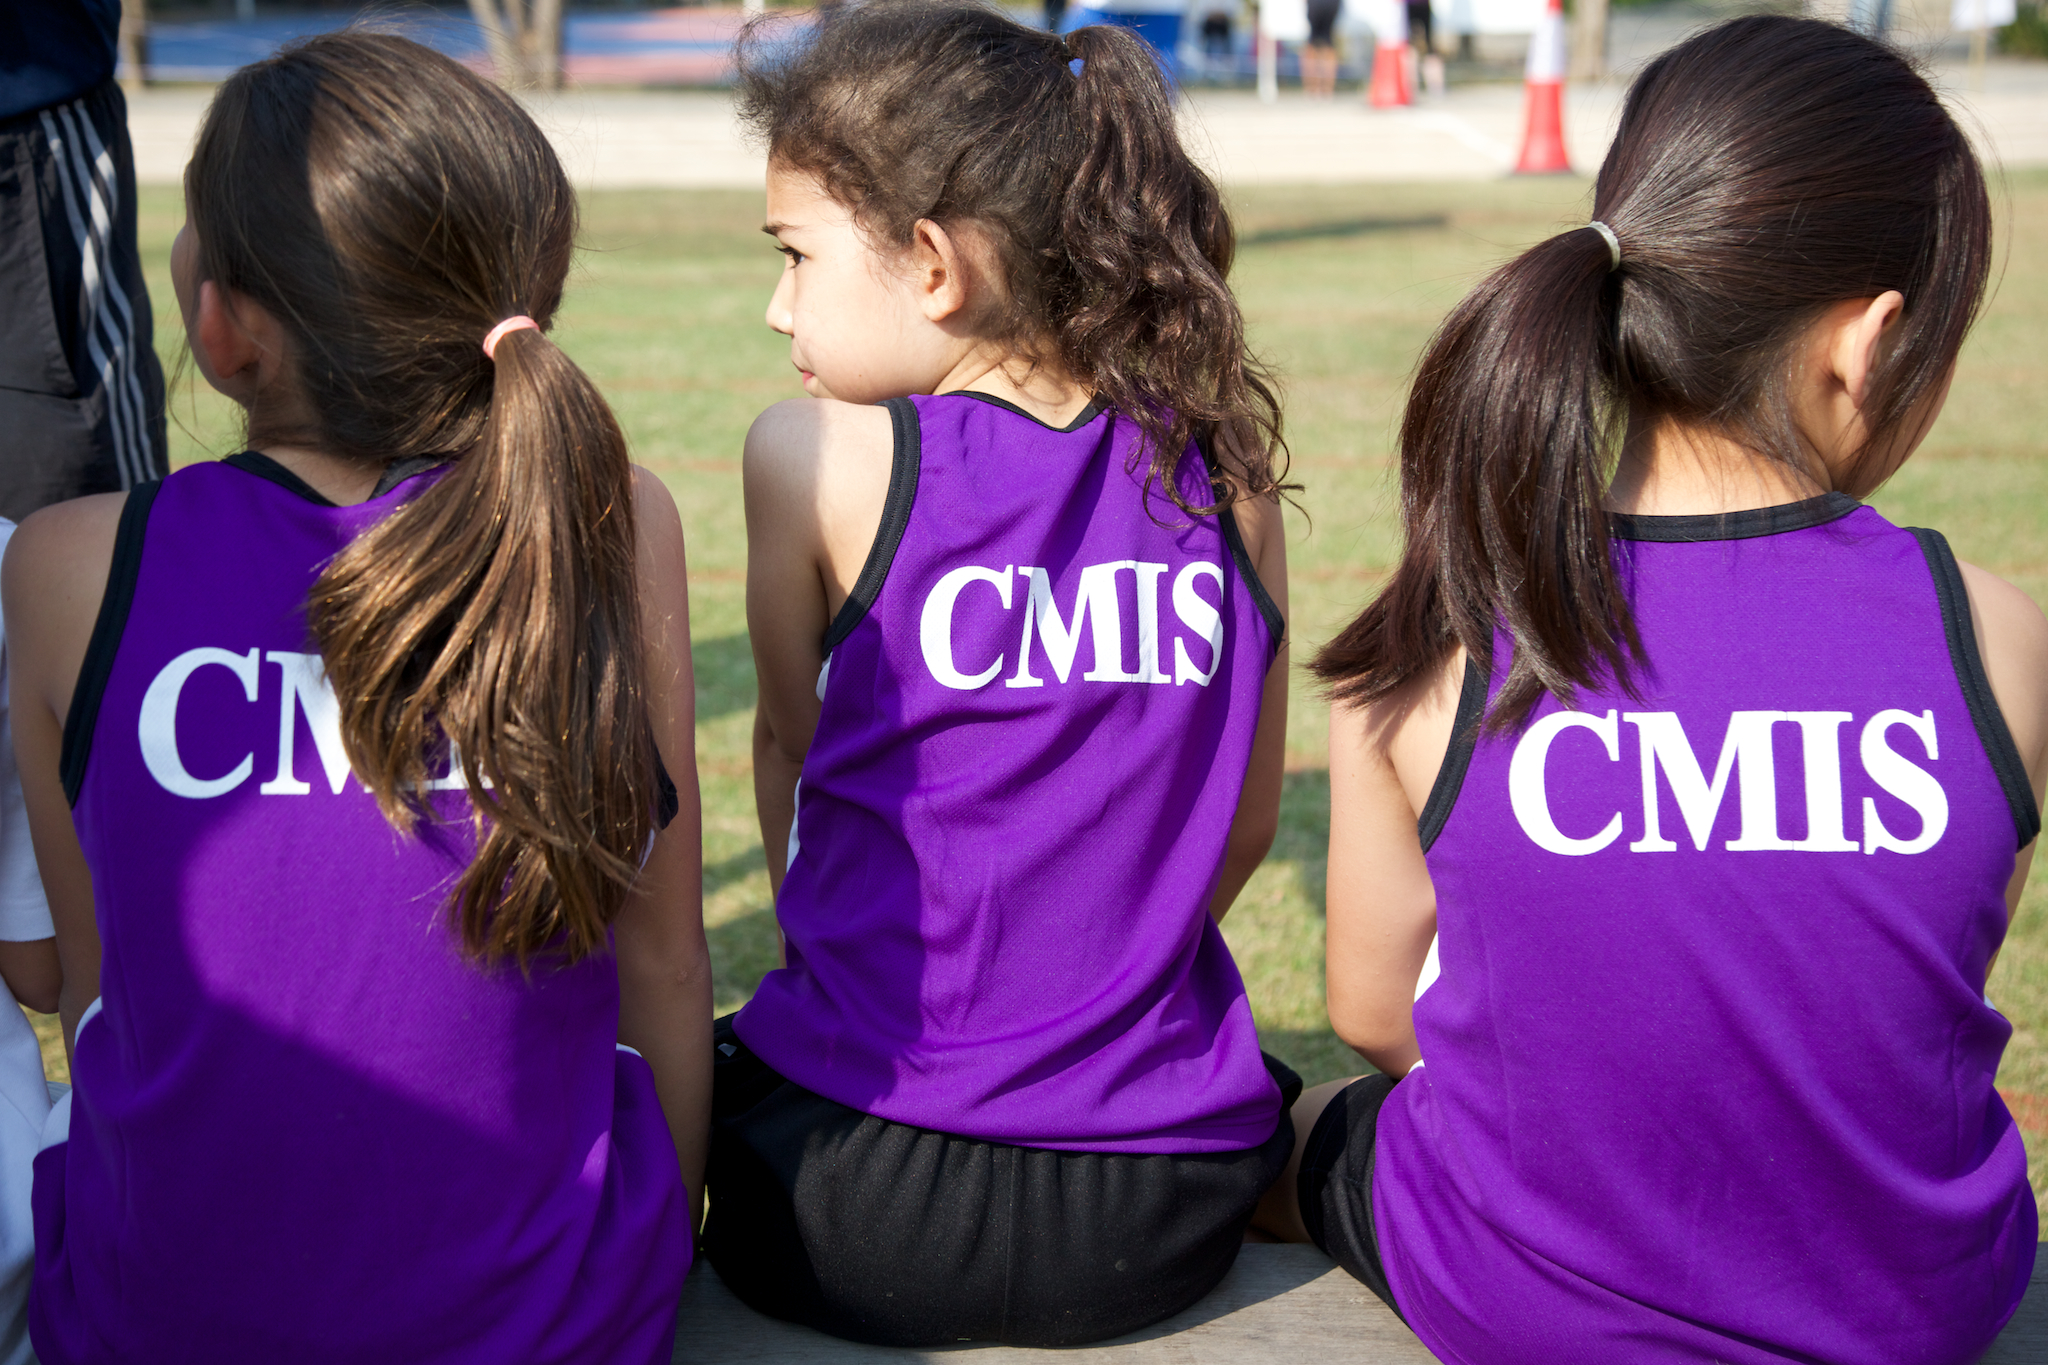
\includegraphics[width=\textwidth]{4_1_1_a.jpg}}

We use globally recognized, research-based standardized tests to identify and assess student needs (e.g, DRA, MAPS, PSAT, and SAT). 

CMIS extracurricular activities (Student Life Beyond The Classroom) emphasize the development of critical thinking skills, the ability to solve problems, and the utilization of effective communication skills. \href{http://blogs.cmis.ac.th/eagles/}{Student Life Beyond the Classroom}

CMIS students participate in community service projects at all three divisions (ES, MS and HS) to promote responsibly in action and service to improve conditions both locally and globally. Examples include Elementary School Thanksgiving Drive for Hope House (local orphanage), \href{https://drive.google.com/a/cmis.ac.th/file/d/0B7jcj1TRcFEGNEtqR3hUSW5QVHM/view?usp=sharing}{Middle School Activity Day} at Hope House and High School \href{http://blogs.cmis.ac.th/community-service/}{community service projects}.

\minor{So what...}

There are many ways in which our school can demonstrate how our vision, mission, and schoolwide learner outcomes have been impacted by pertinent student and community profile data, identified global competencies, and current educational research. 
As our student and community profile is constantly changing, we need to always ensure that we keep abreast of these changes and modify our goals accordingly.
\end{findings}

{\centering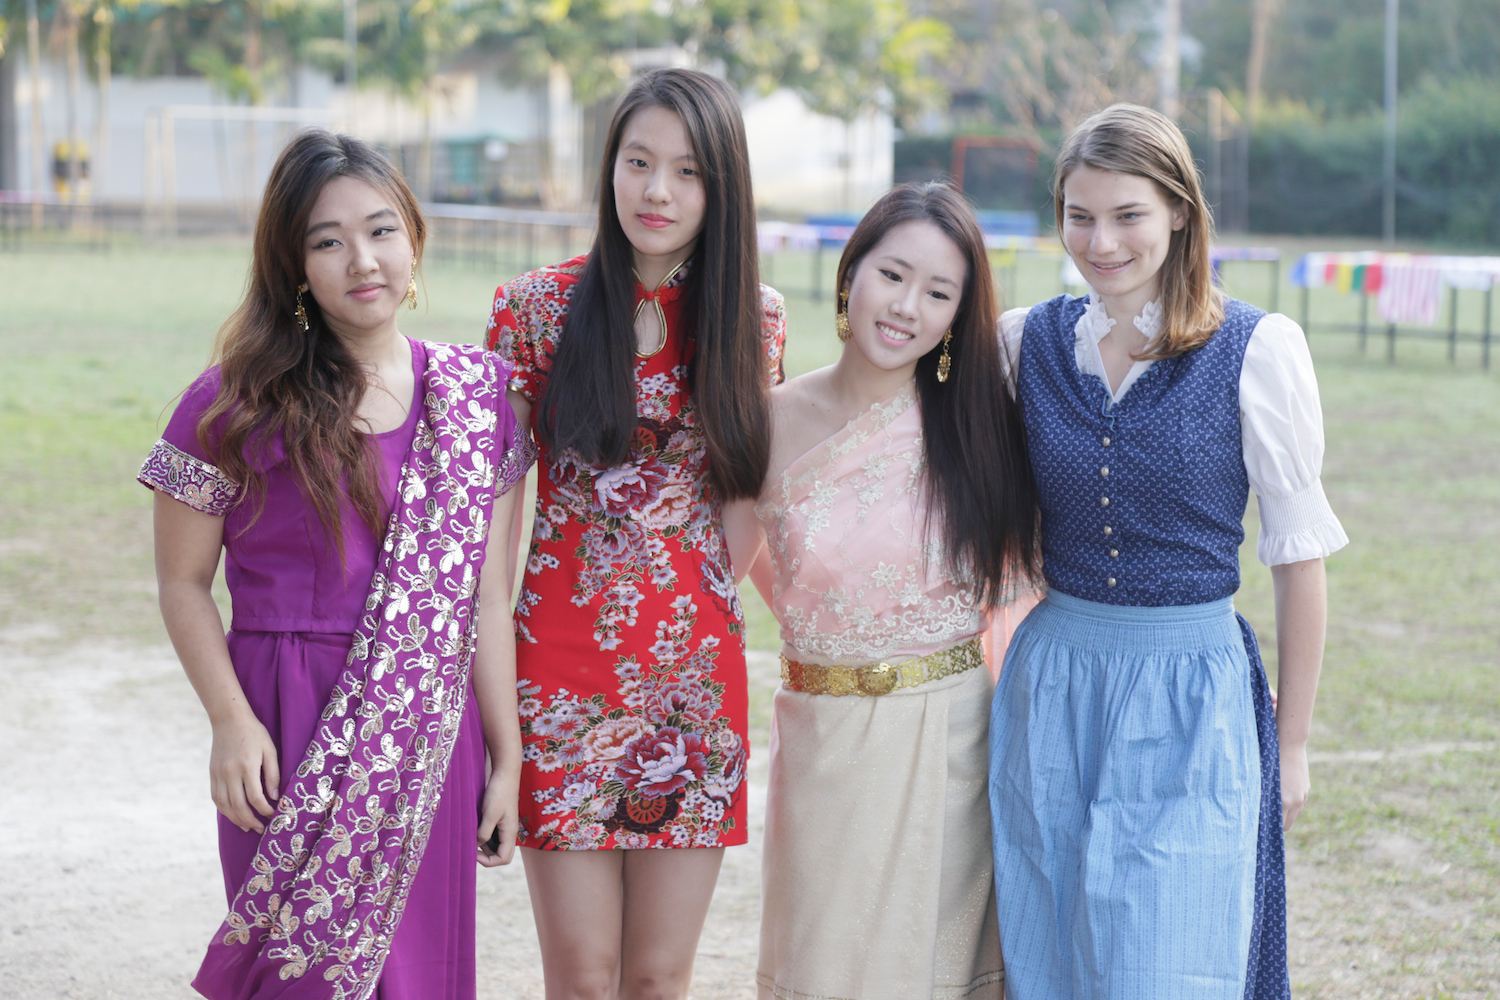
\includegraphics[width=\textwidth]{chapter4_A1.jpg}}

\subsubsection{Involvement of All}

\indicator{The school has a process for involving representatives of the entire school community in the defining of global competencies and in the development/refinement of the core values, mission, vision, and schoolwide learner outcomes.  }

\prompt{Evaluate the processes 1) to ensure the involvement of representatives from the entire school community in the defining of global competencies and the development/refinement of the core values vision, mission, and schoolwide learner outcomes and 2) to determine their effectiveness.}

\begin{findings}
CMIS has several processes for involving representatives of the entire school community in the development/refinement of the core values and schoolwide learner outcomes:

“Teacher Table Talk” sessions are often held during staff development, early release days to capture insights and suggestions about the effectiveness of the CMIS Mission and Student Learner Outcomes.  Example: \href{https://drive.google.com/a/cmis.ac.th/file/d/0ByVFfrm0zfolbHNvSWhVWmJYU3M/view?usp=sharing}{Teacher Table Talk Activity} 

ES students and staff create and participate in monthly \href{https://docs.google.com/a/cmis.ac.th/document/d/1Mv1xjTpbY36naur8SDt9GanKNfR7YtYVL-bWwGLPSHo/edit?usp=sharing}{virtue assemblies} that review and reinforce our school mission, vision and SLO’s. Parents are also invited to attend these events.

{\centering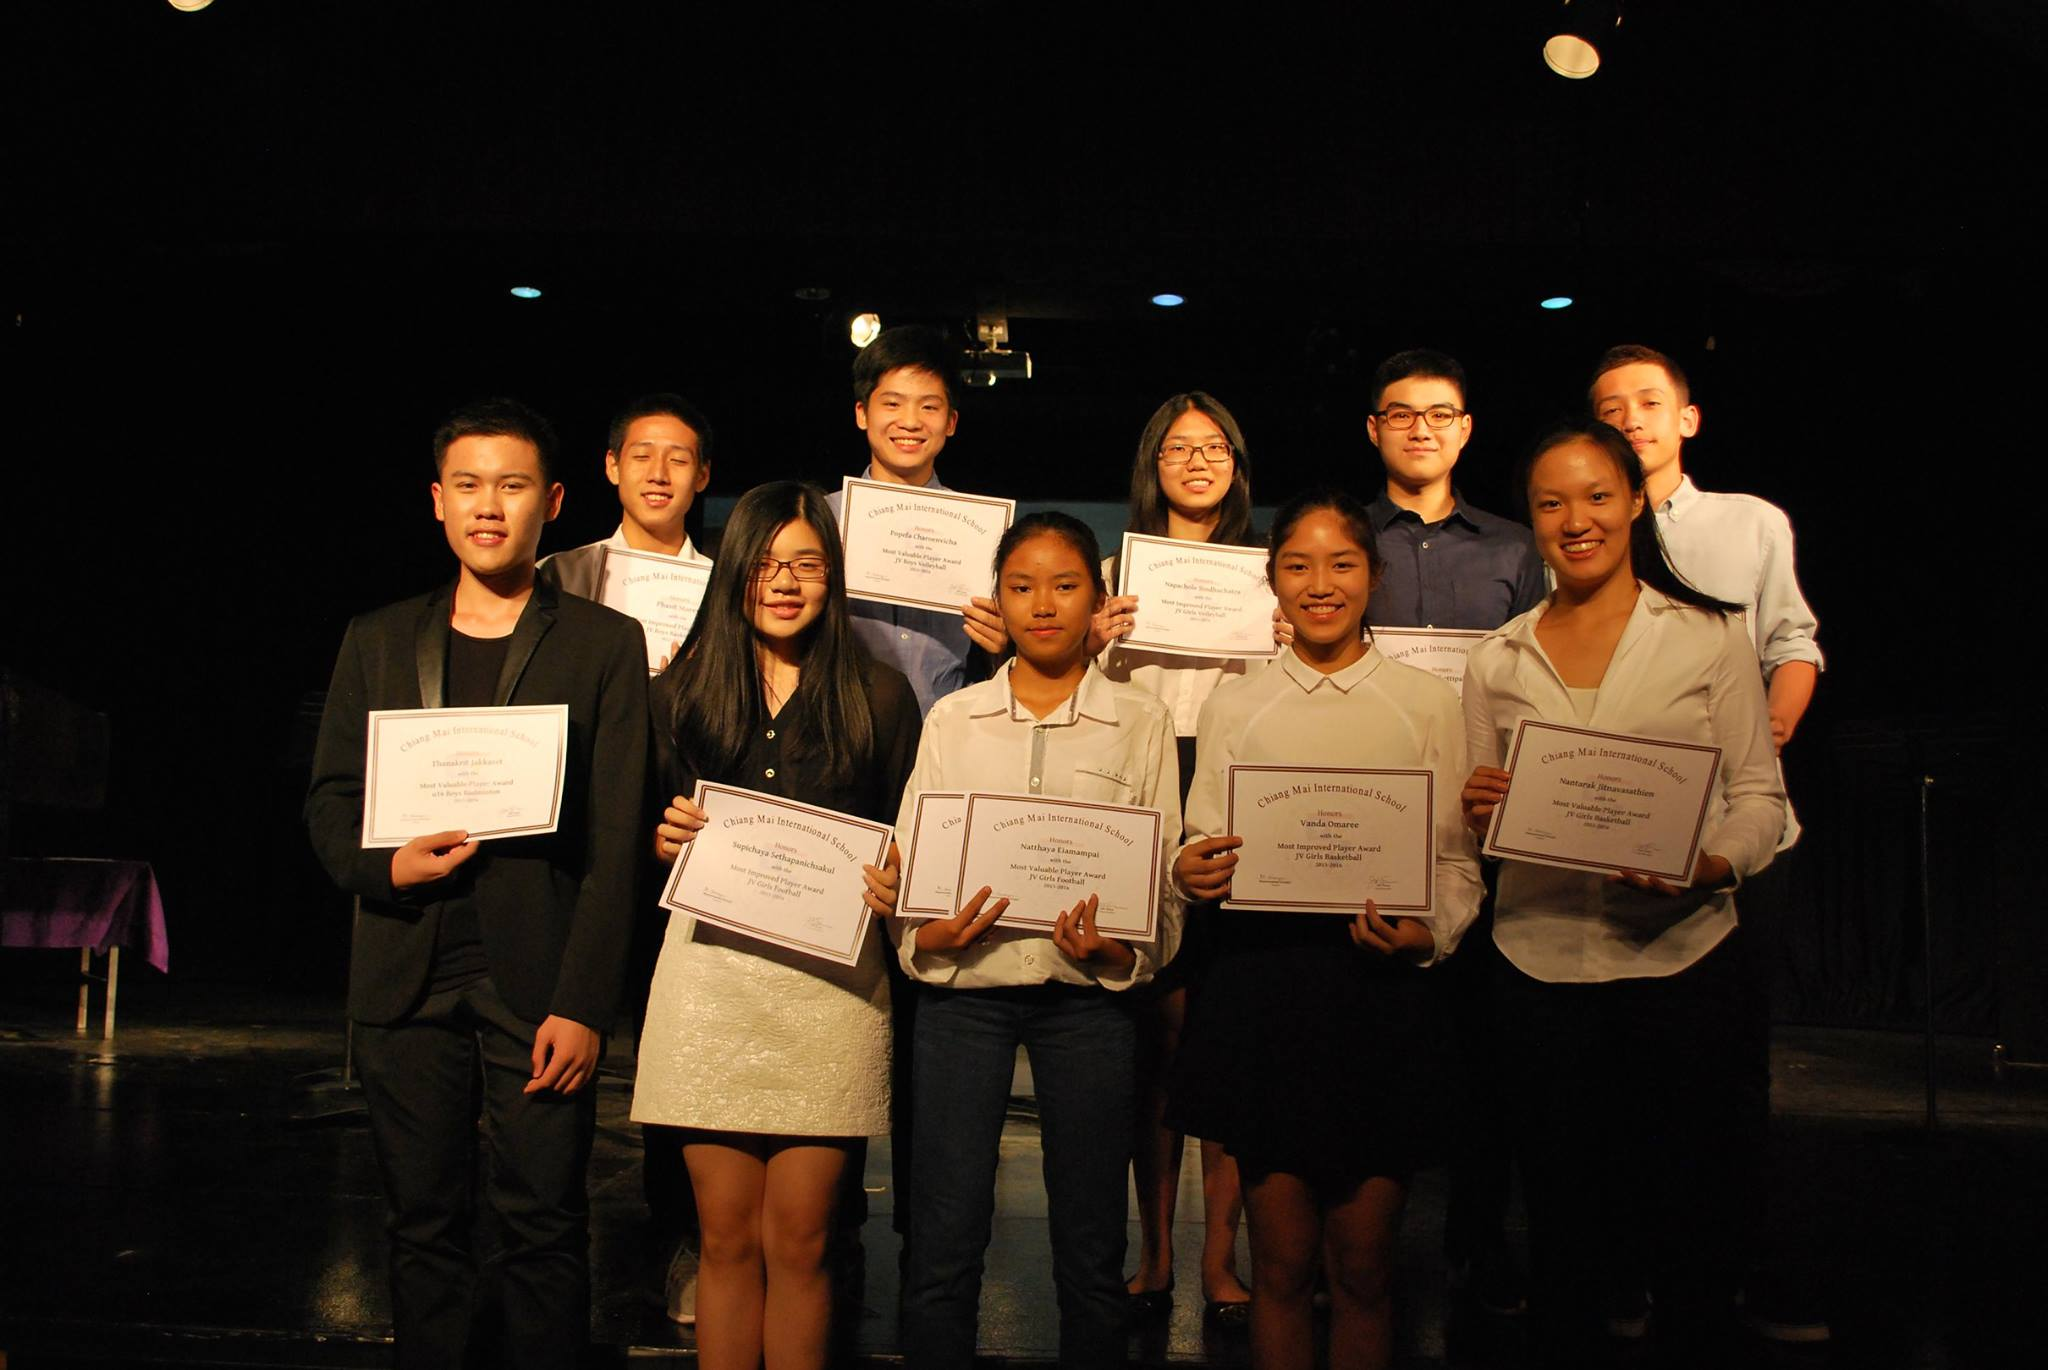
\includegraphics[width=\textwidth]{4_1_1_d.jpg}}

MS and HS Students are encouraged to review our vision, mission, and schoolwide learner outcomes during bi-weekly communication group activities. Communication group have approximately 5-7 students and a teacher leader. This group remains together as a team every year throughout MS and HS.
 
This year, our student learner outcomes posters displayed around campus were designed and created by our grade 6-12 students. \href{https://docs.google.com/a/cmis.ac.th/document/d/1x29XpA7Ro2Xav3JFY0k9F2O22qZi4Yo48hVTYkvhoGM/edit?usp=sharing}{Who We Are Student Poster Competition}.

Several of our student-led clubs involve the defining of global competencies, development/refinement of CMIS core values vision, mission, and schoolwide learner outcomes  (example: CMIS Environmental Club and National Honors Society).

CMIS \href{https://docs.google.com/a/cmis.ac.th/forms/d/16Gbd3MzQOXtjjZ2dG460xw5SHG_eohMIKet3lxYUdAY/prefill}{family surveys} are conducted once a year to solicit feedback from staff, students and parents. The survey gathers data to monitor the effectiveness of CMIS in relation to its mission, vision, and SLO’s. The survey data is analyzed, summarized and used to create goals for improvement. These goals are then shared with each constituency group at the beginning of the year and monitored for progress throughout the year. Example: \href{https://docs.google.com/a/cmis.ac.th/document/d/10w_OSr00xntX42ShaPk4PiNu9FjKP2OgA3g6CKjmEFc/edit?usp=sharing}{Student feedback about cafeteria}.

Our \href{http://blogs.cmis.ac.th/ptg/about/}{CMIS Parent Teacher Leadership Team}- assists and supports the school in the development/refinement of the core values, mission, vision, and schoolwide learner outcomes. This team focuses on this role during monthly meetings with the superintendent, as a leadership team, and during monthly parent meetings that the school management team always attends.

\minor{So what...}

CMIS strives to involve representatives of the entire school community in the development/refinement of the core values and schoolwide learner outcomes.

We believe that we can seek further involvement, and we are trying to reach out and include more involvement with our community-outside of our immediate parent group (examples of progress: reaching out to rotary club and US Consulate).
\end{findings}

\subsubsection{Consistency of Purpose, Schoolwide Learner Outcomes, and Program}

\indicator{There is a strong degree of consistency between the school core values, vision, mission, the schoolwide learner outcomes, and the school program that reflects the school’s explanation of global competencies.}

\prompt{Provide a range of examples that the school vision, mission, schoolwide learner outcomes, and program are consistent. with the school’s explanation of global competencies.}

\begin{findings}
CMIS believes that a global competency doesn't always have to be about world events or other countries, but rather about how to live in the world. Learning how to listen, how to disagree respectfully, how to encourage, and how to collaborate are several elements of a global education that all students need.

The CMIS \href{http://cmis.ac.th/about/vision}{Mission Statement}, \href{http://cmis.ac.th/about/vision}{Student Learner Outcomes}, and school programs are closely related to our goal to equip international students for lives of learning and positive contributions both locally and globally (See \href{http://cmis.ac.th/about/vision}{Who We Are} on website).

CMIS adopted K-12 standards in 2013 that are closely aligned with the school’s mission of academic excellence through rigor, coherence and focus. Our instruction is inquiry-based, which also supports the CMIS key learner outcomes for our students. 

Our grade 6-12 initiative of the 1:1 chromebook reflects our mission to enhance student global proficiency through hands-on, student-centered, and meaningful technology integration. 

Our 2016 \href{https://docs.google.com/a/cmis.ac.th/presentation/d/1xmLAJD96klLrjiBPwCoOMoKmbclYqpIMWaifytzFMgk/edit?usp=sharing}{chromebook survey} results indicated that 73\% of our students felt that the chromebooks increased their ability to demonstrate their learning and 77\% felt that the chromebooks helped them to be more productive. The survey also confirmed how the chromebooks were being used to support essential global competency skills (e,g, presenting, communicating, organizing, researching, and collaborating)

The results of our \href{https://drive.google.com/a/cmis.ac.th/file/d/0B71_pYxcTLo-RlZxQzQyc0NqUFU/view?usp=sharing}{community surveys} confirm that 95\% of our parents parents believe that CMIS provides a high quality education: educational excellence in a caring Christian community that respects and celebrates diversity.

CMIS believes that a global education is not a separate subject or a single lesson; it is a necessary part of all education, for all people. Global education allows a shift in perspective, which provides opportunities for both students and teachers to grow and develop as humans equipped with an understanding of their roles in a complex world.

Some specific teams and staff positions in place to help ensure the promotion of global competency:

\begin{itemize}
\item \href{http://blogs.cmis.ac.th/eagles/}{Student Life Beyond the Classroom} Team
\item Spiritual and Community Service Advisor
\item Spiritual Life Committee
\item \href{http://blogs.cmis.ac.th/ptg/about/}{Parent Teacher Group} Leadership Team
\item Middle School and High School Communication Groups
\item Elementary, Middle, and High School Counselors
\item ES, MS, and HS Student Success Team
\end{itemize}

\minor{So what...}

We have a strong degree of consistency between the school core values, vision, mission, the schoolwide learner outcomes, and the school programs that reflects the school’s explanation of global competencies.

We are trying to move away from the commercial definition of global competency and move towards a more student-centered definition that focuses on authentic opportunities for our community to grow together in a caring community as proactive human beings (i.e. \href{https://drive.google.com/a/cmis.ac.th/file/d/0B0TYmzaZNi3fOF9RQkRqLV9saUE/view?usp=sharing}{Great Kindness Challenge Week}).
\end{findings}

\subsubsection{Communication about Vision, Mission, and Schoolwide Learner Outcomes}

\indicator{The school has means to publicize the \href{http://cmis.ac.th/about/vision}{vision, mission, and schoolwide learner outcomes} to the students, parents, and other members of the school community.}

\prompt{Examine the effectiveness of the means to publicize the purpose and the schoolwide learner outcomes to the students, parents, and other members of the school community.}

\begin{findings}
CMIS has various means to communicate its Vision, Mission Statement and the Student Learner Outcomes to the entire school community:

The CMIS Student Handbook, part of the annual Student Planner, contains information that focuses on our school mission to develop learners who can pursue personal and academic goals, based on academic excellence and strong moral foundations. Link to \href{https://docs.google.com/document/d/1bIbV9pgGz2vpXYJdnRzL_Od5PS35egy7lgBOBuszgD4/edit}{Student Handbook}

Our Vision, Mission and Student Learner Outcomes are displayed prominently throughout campus (examples: student posters and Bible verse banners). 

CMIS publicizes the school vision, mission and student learner outcomes through the CMIS website, accessible to the public and a portal accessible to all parents, students and faculty. It is also included as a footer on all administrative e-mails.  Link to \href{http://cmis.ac.th/about/vision}{Who We Are} on website

School administration always reiterates the school philosophy at all school wide events (e.g. new family orientation, back-to-school night, assemblies). 

As a Christian school, we provide a variety of schoolwide and volunteer opportunities for our community to interact with the Christian ethos, while also respecting the religious diversity of our community (e.g. school-wide Christmas and Easter assemblies, lunchtime bible study groups, and Christian Club Picnic).

Our PTG team reinforces the school vision, mission and student learner outcomes throughout their coffee morning meetings for new families at the beginning of each school year. 

Our board of directors uses the vision and mission in their agenda planning template and uses it as a point of reference throughout their monthly meetings. These meetings are then \href{http://blogs.cmis.ac.th/ptg/public-board-minutes/}{summarized} and shared with our CMIS community on our website.

Our school management team regularly asks for feedback on the effectiveness of our school goals with parents at our PTG meetings, with our staff during our monthly professional development and divisional meetings.

We reflect upon our school goals with our grade 6-12 students during their bi-weekly communications groups and with our elementary students during their and monthly virtue assemblies.

Our teacher leadership team utilize the \href{https://drive.google.com/a/cmis.ac.th/file/d/0ByVFfrm0zfolT25VTjZZRzlXQjA/view?usp=sharing}{meeting wise agenda format} that requires participants to reflect on the objectives of the department meeting in relation to our school goals.

In September a \href{https://docs.google.com/a/cmis.ac.th/presentation/d/1bdi1LZUjWbGKOyB0XR9CGyoY2xLY39SZVKhiHTIJGxc/edit?usp=sharing}{student art competition} was initiated and the student illustration entries were used to better communicate the CMIS vision, mission and student learner outcomes.

Our CMIS weekly newsletter, blogs and \href{https://www.facebook.com/cmis.th/}{Facebook updates} are other effective ways we communicate our Vision, Mission, and Student Learner Outcomes to our community. 

\minor{So what...}

We work hard to publicize the vision, mission, and schoolwide learner outcomes to the students, parents, and other members of our school community.

We are trying to think of more ways of communicating our message in an easier to understand format. Having our students illustrate our philosophy has been very useful, especially with our community members whose english is not their first language.
\end{findings}

\subsubsection{Regular Review/Revision}

\indicator{The school has a process for regular review/revision of the school’s vision, mission, and  schoolwide learner outcomes based on current and future learner needs and other local and global trends and conditions.}

\prompt{Evaluate the effectiveness of the regular process for review/revision of the core beliefs, school vision, mission, and the schoolwide learner outcomes. Include the degree to which the review/revision process addresses current and future learner needs and other local and global trends and conditions.}

\begin{findings}
CMIS has a process for regular review of the CMIS core beliefs based on student needs, global, local needs, and other trends and community conditions.

Our school mission was updated in 2014 and the modified version was formulated by our staff based on current students needs, global and local needs, and other trends and community condition. 

Our Student Learner Outcomes were modified from their original format as Educational Objectives in 2015 to better recognize our diverse community, further embrace students future needs, and include updated global skills. These outcomes were reviewed with the whole community at the beginning of the 2016-2017 school year and student interpretations were displayed as posters across campus. \href{https://docs.google.com/a/cmis.ac.th/presentation/d/1bdi1LZUjWbGKOyB0XR9CGyoY2xLY39SZVKhiHTIJGxc/edit?usp=sharing}{Student Poster Competition}

Each year, CMIS sends an annual community survey (parents, teachers, and students grades 4-12) to solicit perception data related to our effectiveness of implementing our school mission and student learner outcome goals.

\minor{So what...}

As the school’s mission statement and SLOs were recently updated, there has not yet been any rigorous effort to revise them.  However, as CMIS continues to grow and identify innovative ways to enhance teaching and learning, the statement and the SLO’s will be re-evaluated and revised to mirror the diverse needs of our CMIS community.

The CMIS Board has been developing an evaluation instrument for administrators and board members to ensure fidelity to mission, vision, and schoolwide learner outcomes.  Concurrently, the CMIS Board is currently identifying indicators to determine the academic quality and fiscal health of the school. 
\end{findings}

\subsubsection{Conclusions}

\prompt{Comment on the degree to which this criterion is being addressed.}

\begin{findings}

The findings suggest that CMIS addresses this criterion to a high degree. In an effort to increase student achievement further in this area CMIS plans to:

\minor{Maintain and Monitor}

\begin{itemize}
\item Processes and policies that have a strong degree of consistency between the school core values, vision, mission, and the schoolwide learner outcomes.
\item Regular opportunities to continuously communicate school goals with the community
\end{itemize}

\minor{Investigate Better Practice}

\begin{itemize}
\item Ways to communicate CMIS goals in easy to comprehend formats
\item Keeping current with community profile and modifying CMIS goals accordingly.
\end{itemize}

\end{findings}



\subsection{A2 Governance}

The governing authority (a) adopts policies which are consistent with the school’s mission and vision and support the achievement of the schoolwide learner outcomes, i.e., global competencies, (b) delegates implementation of these policies to the professional staff, and (c) monitors results.

\subsubsection{Clear Policies and Procedures}

\indicator{There are clear policies and procedures with regard to the selection, composition, and specific duties of the governing authority.}

\prompt{Evaluate the clarity of the policies and procedures regarding the selection, composition, and specific duties of the governing authority.}

\begin{findings}
The CMIS Board of Directors (the board) has developed clear policies with regard to the selection, composition, and specific duties of the governing authority. 

The board is composed of nine members: four are appointed by the Church of Christ in Thailand (CCT) - our parent organization, three through their role at the school (Director, Manager, Superintendent), one teacher representative, and one parent representative. The teacher representative is elected by the staff and it is preferred (not required) that they serve in a school leadership role (e.g., team leader). They serve for a minimum of two years.

The PTG representative is elected through a process, described further in the \href{http://blogs.cmis.ac.th/ptg/bylaws/}{PTG Bylaws} and serves for a minimum of two years.

Board member roles and responsibilities are clearly outlined and described in the Policies and Procedures Handbook for Administration of the Institutions in the Church of Christ in Thailand

In order to remain current in professional practice, the CMIS Board invited outside consultant John Ritter in September, 2015 to facilitate the discussions on future decisions and outcomes. At this time, the board engaged in a review of its annual goals and the review resulted in a reflection of the school's strengths, weaknesses, threats, and opportunities. 

The board revisited these responsibilities in November 2016 and created a document entitled:  \href{https://docs.google.com/document/d/1EyIeD5g0RDANtZzH5rsCkvDp5ea_bQ2G9rWnhz4QbSc/edit?ts=5881d18d}{Principles of Good Practice}  to better align the board’s responsibilities with the school’s mission, vision, and to further support the achievement of the schoolwide learner outcomes. They also drafted a policy outlining individual board member responsibilities and duties: \href{https://docs.google.com/document/d/14e90Qr4edga9mEZuHIclWeraZ5jgq052IUwcnxTHQZw/edit?ts=5881b471}{Individual Board Member Principles of Good Practice}. These items will be finalized by the board and voted upon for adoption in the February 2017 board meeting.

The board is currently studying the the National Association of International Schools Trustee Handbook (\href{http://www.nais.org/Articles/Pages/NAIS-Trustee-Handbook-Resources.aspx}{NAIS}) together, and using it as a reference for creating future board development.

The board is currently creating a CMIS Board Handbook which is scheduled for compilation by September 2017. This initial version will used as a reference tool for future policies and procedures with regard to the selection, composition, and specific duties of the governing authority. 

\minor{So what...}

The board has focused strongly on adopting policies which are consistent with the school’s mission, vision, and support the achievement of the schoolwide learner outcomes.

Completing the CMIS Board Handbook will allow the BOD to identify additional ways to improve in this area and help to find effective means to communicate these out to our community.
\end{findings}

\subsubsection{Pretraining of Potential Board Members}

\indicator{Individuals who seek board membership or are being considered as appointees by the board will have some form of training in the principles and skills essential to the effectiveness of the school board.}

\prompt{Evaluate the effectiveness of the training that is offered to prospective or new school board members.}

\begin{findings}
CMIS became an official member of the \href{http://www.nais.org/Articles/Pages/NAIS-Trustee-Handbook-Resources.aspx}{National Association of Independent Schools} in 2016 in order to access the most recent research and trends on school governance. 

New CMIS Board members are given a copy of the “International Trustee Handbook of School Board Leaders” to prepare them for their initial tasks of being a CMIS Board member. 

Currently, the CMIS Board utilizes an informal mentoring system where new board members are provided insight and guidance through informal discussions from other senior board members. 

The board chair and newly appointed Superintendent are currently completing book studies together of \textit{Living From the Heart Jesus Gave You} and textit{Joy Starts Here}.Their studies review the Christian ethos, how it relates their own personal journey in Christianity and the Christian vision for CMIS. This mentorship relationship highlights the importance of a strong partnership between the chair and the head of the school,

``It is critical that the chair and head make every effort to establish a solid and mutually supportive relationship based on respect and trust, develop the capacity to be forthright and candid, and listen to and learn from each other's feedback. The board chair and the head share the same goal: providing effective leadership for the school.'' \textit{NAIS Trustee Handbook} p.125

Current and prospective board members have attended EARCOS workshops together for the past two years. Sessions attended by board member at the 2015 EARCOS Leadership Conferences:
\begin{itemize}
\item Learning from Lincoln Leadership
\item Strategic Planning for Effective School Boards 
\item Parent Teacher Organizations: Effective Communication
\item Effective Adoption and Resource Cycles 
\end{itemize}

All board members were asked to review and sign \href{https://docs.google.com/a/cmis.ac.th/document/d/1sVjFjeVtwbk0-n8GsM5K_XzZSn2wejtlJ3kurXUrKGU/edit?usp=sharing}{CMIS Board of Directors: Roles and Responsibilities} of the \href{https://docs.google.com/a/cmis.ac.th/document/d/1sVjFjeVtwbk0-n8GsM5K_XzZSn2wejtlJ3kurXUrKGU/edit?usp=sharing}{Board and CMIS BOD Code of Conduct} at the beginning of the 2016-2017 school year.

\minor{So what...}

The CMIS Board of Directors has worked hard to increase the pre-training and support for new board members but acknowledges that it can do more. The CMIS Board Handbook will include further strategies for new BOD training and support.
\end{findings}

{\centering\includegraphics[width=\textwidth]{chapter4_A2.jpg}}

\subsubsection{Relationship of Policies}

\indicator{The governing authority’s policies are directly connected to the school’s vision, mission and schoolwide learner outcomes that focus on student achievement of global competencies.}

\prompt{Evaluate the adequacy of the policies to support the school’s vision, mission, and schoolwide learner outcomes through its programs and operations.}

\begin{findings}
The CMIS Board models collaborative leadership that provides a unified direction to all leaders and members of the staff. This direction is clearly connected to the school’s purpose evident in its vision, mission, and \href{https://docs.google.com/document/d/1bIbV9pgGz2vpXYJdnRzL_Od5PS35egy7lgBOBuszgD4/edit}{student learner outcomes} (SLOs).

The effective involvement of all stakeholders, starting from the governing authority, in formulating and implementing the vision, mission, and SLOs, ensures that student achievement is the focus of all school decisions. The guidance and leadership of the governing authority provide the momentum necessary to effectively address our vision, mission, and SLOs.

The CMIS Board is responsible for providing the necessary learning programs and operations that support CMIS curriculum and resources, attracting and retaining quality employees, and ensuring the availability of learning materials and supplies. Through the budget funding process, the board also supports professional development for teachers, administrators, support staff, and the board.

At a summer 2016 Board Retreat, the current CMIS Board created a plan for areas of improvement that are based on the following topics: 

\begin{itemize}
\item Stakeholder communications
\item Funds development
\item Strategic planning
\item board handbook
\end{itemize}

The board also developed strategies and procedures to address these areas and are in the process of developing measurable goals to evaluate the effectiveness of these actions. The goals focus on the board’s responsibility to be good stewards of its resources, its fiduciary responsibilities, and on providing clear, strategic leadership to ensure CMIS is viable for years to come.

The CMIS mission, vision, and SLO are consistently integrated into the board agenda template. This is done to ground the meeting in the important work of school outcomes and focus members on our students and their achievement. 

\minor{So what}

CMIS acknowledges that the past decisions and proposals of the board have often been recorded in board minutes that can be difficult to locate and refine. This limits the current board’s ability to effectively evaluate the connectedness of CMIS Board practices, in relation to the the school’s vision and mission.

In an effort to address this challenge, the board has appointed a committee to facilitate the creation of a CMIS Board Handbook, which is scheduled for compilation by September 2017. This Handbook will make it easier for evaluation as the policies will be created in a common format and available in a central location. 
\end{findings}

\subsubsection{Involvement of Governing Authority}

\indicator{The governing authority is involved in the regular review and refinement of the school’s vision, mission, and schoolwide learner outcomes. The governing authority uses a variety of strategies to remain current in research-based knowledge about effective schools.}

\prompt{Evaluate the processes for the involvement of the governing board in the regular review and refinement of the school’s vision, mission, and schoolwide learner outcomes.}

\begin{findings}

The governing authority is involved in the regular review and refinement of the school’s \href{http://cmis.ac.th/about/vision}{vision, mission, and schoolwide learner outcomes}. It also uses a variety of strategies to remain current in research-based knowledge about effective schools.

As mandated by the ``Board of Directors Roles and Responsibilities of the Board'', the board reviews the mission, vision, and schoolwide learner outcomes at the beginning of each school year. For example, in May 2014 the board voted to revise the vision and mission statement, and in 2015 voted to revise the schoolwide learner outcomes so they were more measurable and in line with the Focus on Learning recommendations. 

In order to remain current in research based knowledge about effective schools, the CMIS Board invited outside consultant John Ritter in September, 2015 to facilitate board development  that reviewed the characteristics of effective school boards. In summary, the workshop focused on:

\begin{itemize}
\item Having a shared vision about high capabilities of both students and staff
\item Being policy and accountability driven
\item Engaging in goal-setting processes that can drive action in the school to improve
\item Aligning resources around those goals
\item Using data to diagnose problems and to monitor and drive continuous improvement efforts
\item Communicating and engaging with the community
\item Working well together as a team 
\end{itemize}

These characteristics have been used as the foundation for CMIS Board planning and will provide the framework of the CMIS Board Handbook. The board chair also studied the book, \href{https://www.amazon.com/Governance-Leadership-Reframing-Nonprofit-boards/dp/0471684201}{\textit{Governance as Leadership}}  which reviews the process of generative thinking in relation to strategic planning and plans to also use the guidelines from this research based book in the compilation of the CMIS Board Handbook.

CMIS is a member of The International School Association of Thailand (ISAT). ISAT works with government ministries to keep current of the benefits of international education in Thailand and promotes quality international school education.

The quality of education offered at the ISAT member schools has been recognized by accreditation organizations such as the \href{https://en.wikipedia.org/wiki/Western_Association_of_Schools_and_Colleges}{Western Association of Schools and Colleges} (WASC), and the \href{https://en.wikipedia.org/w/index.php?title=Council_of_International_Schools&action=edit&redlink=1}{Council of International Schools} (CIS).

The CMIS Superintendent and Manager serve on the CMIS Board and attend the \href{https://drive.google.com/a/cmis.ac.th/file/d/0Bwny3HLdIIS7LUtqTlR2REhsLVBkWHVib3k3V1hsWVFtUzIw/view?usp=sharing}{ISAT quarterly meetings} together. It is a great opportunity to review the CMIS vision, mission, and schoolwide learner outcomes in relation to other schools in Thailand. 

At the ISAT meetings there are often guest speakers (e.g., in November, Dr. Chaipreuk Sereerak, Permanent Secretary, Ministry of Education and Mr. Krittachai Aroonrat, Secretary General, Office of Private Education Commission) . Their expertise and guidance assist the board in remaining current about effective schools international school policy and educational trends in Thailand (\href{http://www.isat.or.th/members/announcement-updates/minutes-isat-general-member-meeting-22016}{sample minutes}).

CMIS Manager, \href{https://drive.google.com/a/cmis.ac.th/file/d/0Bwo-i12FeO0rY1V1SGtuSzJBd1U/view?usp=sharing}{Patcharin Jingkaojai} was elected in 2016 to the ISAT Management Committee which provides leadership and support to membership schools throughout Thailand. In September 2016 the Management Committee organized the \href{https://drive.google.com/a/cmis.ac.th/file/d/0Bwo-i12FeO0rQ0JOZ09JVTNEUTA/view?usp=sharing}{Regional Member Meeting} that was hosted at CMIS. 

In 2016, the CMIS Superintendent, Nel Capadona joined the ISAT Professional Development Committee and assists with supporting professional development, school development, and networking for ISAT member schools. In November 2016 they promoted the \href{https://drive.google.com/a/cmis.ac.th/file/d/0ByVFfrm0zfolSXFEZFJVN1VOaTQ/view?usp=sharing}{EARCOS Focus, Coherence and Rigor Math Workshop} that was hosted by CMIS.

\minor{So what...}

The CMIS BOD works hard to regularly review and refine the school’s vision, mission, and schoolwide learner outcomes. 

The board is currently completing a book study together of the \textit{International Trustee Handbook of School Board} (NAIS). The handbook has been a valuable resource on reflecting upon how to effectively review and refine school goals. The board plans to complete their own handbook by September 2017 and use it as the foundation for future BOD strategic planning.

\end{findings}

\subsubsection{School Community Understanding}

\indicator{ The school community understands the governing authority’s role.}

\prompt{To what degree does the school community understand the governing authority’s role?}

\begin{findings}
The CMIS Board ensures community understanding of their role through a variety of means. 

The board works hard to adhere to the best practice that, ``An effective board keeps its most important records of business up-to-date and ensures that they are accurate, concise, and timely'' (Devarics, 2011).

For example:

board agendas are planned by the school executive team with the board chair and sent out to all board members a week before the monthly board meeting for review and comment. 

board minutes are kept by the board secretary, approved at the next meeting and summarized for the community on the PTG website. The meeting summaries are also referenced by the superintendent at the monthly PTG meetings. \href{http://blogs.cmis.ac.th/ptg/public-board-minutes/}{Public board minutes on PTG Blog}

Currently, the CMIS Board is developing a CMIS Board Handbook to ensure a clearer understanding of the relationship between the governing authority and the community. The board is using the National Association of International Schools (\href{http://www.nais.org/Articles/Pages/NAIS-Trustee-Handbook-Resources.aspx}{NAIS}) Trustee Handbook as a research based reference for this project: Chojnacki, David. \href{https://www.nais.org/Bookstore/Pages/ProductDetail.aspx?productid=\%7B47CD9104-BC67-E111-9A8C-00505683000D\%7D}{INTERNATIONAL Trustee Handbook: A Guide for Effective Governance for Independent School Boards}. 

Though the board clearly understands the limits of the board/community relationship, the CMIS Board is working hard to increase opportunities to formally and informally interact with the community to ensure that, “...the school is fulfilling its mission with vision and energy, [and that] all  of the school’s constituents will be bound together by this mission (NAIS Trustee Handbook, Chojnacki, 139)  

Examples:

Formal opportunities to interaction with Parents include:
\begin{itemize}
\item board members attend parent \href{https://drive.google.com/a/cmis.ac.th/file/d/0Bwny3HLdIIS7d1FGeDhaZE1EcG1PMHlMX2NRZTdIYXlWZERB/view?usp=sharing}{coffee mornings} at start of the school year
\item board members attend and speak at \href{https://drive.google.com/a/cmis.ac.th/file/d/0Bwny3HLdIIS7NGpoVEtlWmw2RE0/view?usp=sharing}{Senior Graduation day}
\item board members welcome at New Family Orientation Day
\end{itemize}

Informal opportunities to interact with Parents include:
\begin{itemize}
\item board members attend monthly PTG Meetings
\item board members sponsoring student organizations (e.g. \href{https://drive.google.com/a/cmis.ac.th/file/d/0Bwny3HLdIIS7WXpial9KYjFlWFBBQW1YQ2thOVpsTTFCeGVr/view?usp=sharing}{Boy Scouts})
\item board members mingle with families during Welcome Back BBQ
\item board members attend Social school events (Latin Night, CMIS Invitational Basketball Tournament, etc.)
\end{itemize}


Recent CMIS \href{https://docs.google.com/a/cmis.ac.th/document/d/1_otvw47y3Z-1CSjXnKhgRTauVRqPl1S6nSdmsb00O2k/edit?usp=sharing}{family survey results} indicate that the majority of our community believe that the CMIS Board communicates effectively with the community and that our ratings have increased in this area over the last two years.

This year, in an effort to increase the board's communication efforts further CMIS has included photos and provided backgrounds of our board members and their board roles on our school website. We have generated \href{https://drive.google.com/a/cmis.ac.th/file/d/0Bwny3HLdIIS7MjJMX1ZIVS1zSXJOaTNZcFRmTWV1Q1VTc1hZ/view?usp=sharing}{annual community letters} from the board chair and our School Executive Team updating the community of our current goals and our appreciation for their support.

\minor{So what...}

The board has devoted time and resources to improve in this area but there is always room for additional communication. They plan to do this by:

Including more specific questions about the board’s effectiveness in next year’s community survey. 

Changing the response format to make data analysis easier to correlate and manipulate. The current ``neutral'' option makes responses difficult to interpret.
\end{findings}

\subsubsection{Relationship to Professional Staff}

\indicator{There is clear understanding about the relationship between the governing authority and the responsibilities of the professional staff. The governing authority limits its actions to policy making and strategic planning — authorizing the administration to implement its decisions.}

\prompt{Determine whether there is clear understanding about the relationship between the governing board and the responsibilities of the professional staff and how that understanding is developed and maintained.}

\begin{findings}
\href{https://docs.google.com/a/cmis.ac.th/document/d/1_otvw47y3Z-1CSjXnKhgRTauVRqPl1S6nSdmsb00O2k/edit?usp=sharing}{Data} indicates that there is a clear understanding about the relationship between the governing board and the responsibilities of the professional staff and how that understanding is maintained. 

During the 2016-2017 Board Retreat the board reviewed the Board of Directors Roles and Responsibilities and The Board Code of Conduct. These documents clearly define the board responsibilities in relation to the CMIS staff and community. In an effort to increase understanding these documents have been made available for review on the CMIS website.

Currently, the CMIS Board is developing a CMIS Board Handbook to ensure a clearer understanding of the relationship between the governing authority and the professional staff. The board is using the National Association of International Schools Trustee Handbook as a research based reference for this project: Chojnacki, David (\href{http://www.nais.org/Articles/Pages/NAIS-Trustee-Handbook-Resources.aspx}{NAIS}). \href{https://www.nais.org/Bookstore/Pages/ProductDetail.aspx?productid=\%7B47CD9104-BC67-E111-9A8C-00505683000D\%7D}{INTERNATIONAL Trustee Handbook: A Guide for Effective Governance for Independent School boards}. 

Though the board clearly understands the limits of the board/faculty relationship, the CMIS Board is working hard to increase opportunities to formally and informally interact with faculty to ensure that, “...the school is fulfilling its mission with vision and energy, [and that]  all  of the school’s constituents will be bound together by this mission (NAIS Trustee Handbook, Chojnacki, 139)  

Examples:
Formal opportunities to interact with Administrators and Faculty:
\begin{itemize}
\item board members participating in FOL/WASC focus groups (early release days)
\item board members attending New Teacher Orientation
\item board Chair providing Welcome Back Blessing at beginning of the school year. 
\item board presenting at Teacher Appreciation and Farewell Staff Luncheon 
\item board members leading prayer during school-wide assemblies.
\end{itemize}

Informal opportunities to interact with Administrators and Faculty: 
\begin{itemize}
\item board members attending school fundraisers (e.g., Latin night)
\item board members attending school performances
\item board members attending social and sporting events
\item board members providing spiritual guidance to volunteer staff members
\end{itemize}

\minor{So what...}

The board has worked hard to define the relationship between the governing authority and the responsibilities of the professional staff. The BOD has tried to limit its actions to policy making and strategic planning — authorizing the administration to implement its decisions.
\end{findings}

\subsubsection{board Evaluation/Monitoring Procedures}

\indicator{There is clarity of the evaluation and monitoring procedures carried out by the governing board, including the review of student performance, overall school programs and operations, and the fiscal health of the school.}

\prompt{Determine the degree to which there is clarity of the evaluation and monitoring procedures carried out by the governing board, including review of student performance, overall school programs and operations, and fiscal health of the school.}

\begin{findings}
The board participates in regular evaluation and monitoring procedures, including the review of student performance, overall school programs and operations, and the fiscal health of the school.

The CMIS School Executive Team (\href{https://drive.google.com/a/cmis.ac.th/file/d/0Bwny3HLdIIS7di1mY0xFMnJyWmQzNEhON09EREpvY0JRd0Jv/view?usp=sharing}{Manager, Superintendent, and Director}) present monthly \href{https://docs.google.com/document/d/1gz3SiCiPUMU9n-JgGqzGQhgl0r0qAdpSfQPtBK-rwyI/edit}{SET} reports to the board that include updates on specific elements of school performance, programs, development, operations, and fiscal health. The Superintendent focuses on clarifying admission trends, evaluating academic excellence, demonstrating achievement, reviewing professional development projects, and providing updates on accreditation. The Director focuses on sharing initiatives to ensure compliance with Thai regulations (i.e. ONESQA) and the CCT spiritual growth initiatives (example: \href{http://blogs.cmis.ac.th/spiritual-life/2017/02/03/the-lords-prayer-weekly-devotional-60217-100217/}{The CMIS Lighthouse: Weekly Devotion}). Finally, the Manager ensures that appropriate financial audits are completed for CCT monitoring, and that fiscal procedures and resources are being used with fidelity. 

Beginning in 2015, the board began to send out a \href{https://docs.google.com/a/cmis.ac.th/document/d/16DVRIWxzKBgzVMqk8coHlO97SFWthAA_DEx4z6WSHQs/edit?usp=sharing}{Community Report} that reviews student performance, overall school programs and operations, and the campus development of the school each semester.  

As part of the 2015 and 2016 annual board Retreat, a report and evaluation of student performance, programs, and teacher professional development was part of the board planning for the upcoming year. 

Currently, the CMIS Board is completing a book study together of the research-based (\href{http://www.nais.org/Articles/Pages/NAIS-Trustee-Handbook-Resources.aspx}{NAIS}) Trustee Handbook.  Based upon the findings of this reference tool, one of the 2016-2017 board goals is to communicate this evaluation to our community at the end of this year in the form of a CMIS Annual Report.

\minor{So what...}

Currently, the board implements monitoring and evaluation processes based upon perceptual data only. Though this is useful and helpful data, the board would like to begin collecting more quantitative data to help make governance decisions, such as: student data that is aligned to adopted standards and data that correlates to specific school programs and operations and fiscal health indicators. 
\end{findings}

\subsubsection{Complaint and Conflict Resolution Procedures}

\indicator{The established governing board/school’s complaint and conflict resolution procedures as they apply to the school’s stakeholders are effective.}

\prompt{Comment on the effectiveness of the established governing board/school’s complaint and conflict resolution procedures as they apply to the school’s stakeholders.}

\begin{findings}
CMIS has clear complaint and conflict procedures in place to work through unresolved situations, where an action or decision may be considered unfair or inappropriate.  

There is an anonymous process for teachers to share concerns with administration through the Teacher Administration Communication Team (\href{https://docs.google.com/a/cmis.ac.th/document/d/14nhwcw8xo3i-23Q-WUxo6KJ_c8yFKu-jTdCctt4MFcs/edit?usp=sharing}{TACT}) that meets monthly to review and address current staff concerns. The concerns are addressed collaboratively and a \href{https://docs.google.com/a/cmis.ac.th/document/d/1KLB4c5_LkxXzq4vP2EuNhBVPp2q_FT9qy1cBBwaS5JM/edit?usp=sharing}{summary} of the solutions and suggestions are e-mailed out to all staff.

If teachers have concerns related to their students, they are encouraged to reach out to the Student Success Team facilitated by our Student Service Coordinator.  There is a \href{https://docs.google.com/a/cmis.ac.th/forms/d/e/1FAIpQLScVtFtaEXarGOjwsiJyGdbLAMbeNzG9m44i1fWXFLbtMKZcUg/viewform}{Student Service Request Form} available on the teacher dashboard section of the CMIS website. This form activates immediate support from the divisional counselor to meet with the teacher and create a plan of action.

There is also a formal structure in place with regard to resolving internal conflicts between teachers and administration through the board of directors (\href{https://docs.google.com/a/cmis.ac.th/document/d/1RRBuWgqIb-BlwD8vTRrTG0u_FCHgQFD_oEbvseNdAPc/edit?usp=sharing}{Staff Grievance Policy}). This policy is included in the \href{https://docs.google.com/document/d/1fNreQp5yTOg_g9K4UnR8xvyQf-GcFOHo-6Onp4SqlKg/edit}{CMIS Faculty Handbook}.

Parents with student or school concerns are directed to page 26 of the Student Planner: Communication between School and Home, which contains the process of communicating issues with the school.
Parents are also encouraged to share their concerns or suggestions with the superintendent during the weekly '\href{http://blogs.cmis.ac.th/newsletter/2016/09/05/super-thursdays-starts-this-week/}{Super Thursdays}' or a \href{http://blogs.cmis.ac.th/ptg/about/}{PTG Leadership Team} member at any time. 

\minor{So what...}

The CMIS Board will continue to monitor and maintain the programs and processes that are in good standing. There are areas of growth in this section, for example: the community suggested creating a Sounding Board Session where members from the community (i.e. students, parents, teachers) can meet with the board in an informal setting to discuss concerns and suggestions. CMIS looks forward to piloting this process in March 2017
\end{findings}

\subsubsection{Evaluation Procedures}

\indicator{The governing authority carries out clearly defined evaluation procedures.}

\prompt{Comment on the clarity of the evaluation procedures carried out by the governing authority.}

\begin{findings}
The School Executive Team (Manager, Superintendent, and Director) presents monthly \href{https://docs.google.com/document/d/1gz3SiCiPUMU9n-JgGqzGQhgl0r0qAdpSfQPtBK-rwyI/edit}{School Executive Team Reports} to the board that include updates on specific elements of school performance, programs, professional development, operations, and fiscal health. 

As part of the 2015 and 2016 annual \href{https://drive.google.com/a/cmis.ac.th/file/d/0B-CVlEN-TDChSTJ6QzdQQUczT0k/view?usp=sharing}{Board Retreat}, a Strength, Weakness, Opportunities and Threats (\href{https://drive.google.com/a/cmis.ac.th/file/d/0B-CVlEN-TDChNVJudnJBNnZveTQ/view?usp=sharing}{SWOT}) analysis was completed. The purpose of a SWOT analysis is to identify:

\begin{description}
\item [Strengths] Factors that are likely to have a positive effect on (or be an enabler to) achieving the CMIS objectives.
\item [Weaknesses] Factors that are likely to have a negative effect on (or be a barrier to) achieving CMIS objectives.
\item [Opportunities] External factors that are likely to have a positive effect on achieving or exceeding CMIS objectives, or goals not previously considered.
\item [Threats] External factors and conditions that are likely to have a negative effect on achieving CMIS objectives, or making the the objective redundant or unachievable.
\end{description}

During the 2016 retreat the board also created goals based on feedback from a \href{https://docs.google.com/a/cmis.ac.th/document/d/1QoHZUrC_PbxitA2t_ZGH8DidxTLVe46HSl9otFPnE4k/edit?usp=sharing}{community perception survey} that was studied to evaluate what is effective and less effective CMIS programs, systems and procedures.

Beginning in 2015, the board began to send out \href{https://docs.google.com/a/cmis.ac.th/document/d/16DVRIWxzKBgzVMqk8coHlO97SFWthAA_DEx4z6WSHQs/edit?usp=sharing}{Community Plan Updates} that reviewed student performance, overall school programs and operations, and the fiscal health of the school each semester.  

\minor{So what...}

The CMIS Board has spent time and effort identifying the school’s strengths, weaknesses, opportunities, and threats. This year, the board has developed strategies and processes to maximize the strengths and opportunities and diminish the threats and weaknesses detailed from the SWOT analysis. The board is currently in the process of reviewing the implementation of these strategies. After the review, the board will monitor and maintain those strategies that are effective and modify those that could be improved. These committees are outlined in the section entitled: Relationship of Policies. 
\end{findings}

\subsubsection{Evaluation of Governing Authority}

\indicator{There is a process for evaluating the governing authority.}

\prompt{Review and assess the process for evaluating the governing authority}

\begin{findings}
The board currently uses \href{https://docs.google.com/a/cmis.ac.th/document/d/1_otvw47y3Z-1CSjXnKhgRTauVRqPl1S6nSdmsb00O2k/edit?usp=sharing}{CMIS community survey results} to evaluate the board’s effectiveness as a collective group as well as the Superintendent as a leader. 2016 data indicates that the majority of our parents believe that the CMIS Board and school leadership are effective.

The CMIS Board is currently completing a Due Diligence Checklist based on the guidelines included in the International Trustee Handbook: A Guide for Effective Governance for Independent School Boards (Chojnacki).The checklist will be used to complete an internal evaluation by the board that can be used in conjunction with the family survey results to create meaningful goals for for future board improvement.

The board chair and newly appointed Superintendent are working together to create a comprehensive Superintendent evaluation instrument and process. They plan to present the research based model to the board in April for review and adoption for the 2017-2018 school year.

\minor{So what...}

The board acknowledges that this is an area for future board improvement and that additional data sources should be used for board evaluation. It also realizes that the current community survey format should be modified to increase usefulness. Eliminating the “neutral “ option, preventing questions from being skipped and adding more specific questions related to the boards effectiveness are being implemented in this year’s April survey.
\end{findings}

\subsubsection{Conclusions}
\prompt{Comment on the degree to which this criterion is being addressed.}

\begin{findings}
The findings suggest that CMIS addresses this criterion to a high degree. In an effort to increase student achievement in this area the CMIS Board plans to:

\minor{Maintain and Monitor}
\begin{itemize}
\item Processes and policies that focus on the CMIS Vision, Mission, and Schoolwide Learner Outcomes
\item Compilation of the CMIS Board of Directors Handbook
\item Completion of the NAIS Trustee Handbook board book study
\end{itemize}

\minor{Continue to Improve}

\begin{itemize}
\item Increased communication with stakeholders regarding board roles and CMIS achievement
\end{itemize}

\minor{Investigate Better Practice}

\begin{itemize}
\item To find additional ways to evaluate board effectiveness outside of perceptual data. 
\end{itemize}
\end{findings}

\subsection{A3 School Leadership}
The school leadership (1) makes decisions to facilitate actions that focus the energies of the school on student achievement of the schoolwide learner outcomes, i.e., global competencies, (2) empowers the staff, and (3) encourages commitment, participation, and shared accountability for student learning in a global environment.

\subsubsection{Defined Responsibilities, Practices, etc.}

\indicator{The school has administrator and faculty written policies, charts, and handbooks that define responsibilities, operational practices, decision-making processes, and relationships of leadership and staff.}

\prompt{Evaluate these administrator and faculty written policies, charts, and handbooks. Determine the clarity and understanding of these by administration and faculty.}

\begin{findings}
CMIS has clear policies that define responsibilities, operational practices, decision making processes and relationships of leadership and staff. 

These policies and procedures can be found in the CMIS employment contracts and the \href{https://drive.google.com/a/cmis.ac.th/file/d/0ByVFfrm0zfolVm9uc19UNl82NVpPMUZ1ZEstZlFidEY1c2hn/view?usp=sharing}{CMIS Faculty Handbook}. They are reviewed annually during the administrative, new teacher, and returning staff orientations. 

Furthermore, a list of administrative teams is included in the Faculty Handbook and CMIS Student Planner. 

CMIS organized ``\href{https://drive.google.com/a/cmis.ac.th/file/d/0ByVFfrm0zfolbHNvSWhVWmJYU3M/view?usp=sharing}{Teacher Table Talk}'' sessions during early release days to capture insights and suggestions about the decision-making processes and relationships of leadership and staff. 

In November, 2016 the \href{https://docs.google.com/a/cmis.ac.th/document/d/1iW_tWIwRlWU2p0oIOvd3usDsxj9qYDt_2ROwNPBTHSc/edit?usp=sharing}{Teacher Leadership Team}  which is made up of teachers and administrators, participated in the revision of the handbook format and made it available in an electronic formatted version. We plan to make this an annual project as it was previously revised only by administrators.

CMIS Board governance requires the School Executive Team (i.e. Superintendent, Director and Manager) to maintain up-to-date operational handbooks and procedural guidelines.

Board member roles and responsibilities are clearly outlined and described in the \textit{Christian Churches of Thailand Board Handbook}.

\minor{So what...}

CMIS Leadership has clearly defined roles for teachers only through a variety of methods, most notably the Teacher Handbook. CMIS should continue to maintain, monitor, and modify, as necessary, the Teacher Handbook with stakeholder feedback and input. Additionally, CMIS should develop a Leadership Handbook to clearly outline the roles and responsibilities of principals, directors, and team leaders.
\end{findings}

\subsubsection{Existing Structures}

\indicator{The school has existing structures for internal communication, planning, and conflict resolution.}

\prompt{How effective are the existing structures for internal communication, planning, and conflict resolution?}

\begin{findings}

CMIS has many existing structures for internal communication, planning, and resolving differences.

Communication and Planning Examples:
The School Executive Team (SET) shares information from the monthly Board of Director Meetings to the School Management Team (SMT), and to the \href{https://docs.google.com/a/cmis.ac.th/document/d/1iW_tWIwRlWU2p0oIOvd3usDsxj9qYDt_2ROwNPBTHSc/edit?usp=sharing}{Teacher Team Leaders} who communicate the information to the teachers.

Internal communication is also highlighted through Weekly \href{https://docs.google.com/a/cmis.ac.th/document/d/1Jh_VpJ8rfb4_OwmpRw6VZCrIYAuV6A0SP_3NN82KD7A/edit?usp=sharing}{HS Principal Notes}, MS Principal Message and ES Principal Notes that are sent electronically to all staff.

The Superintendent and principals are out on campus every morning before school for personal communication with students, parents and staff.

The Superintendent and principals meet weekly to address any community concerns and plan.

Additionally, e-mails, memos, google docs are used to further enhance communication.

\minor{Communication Examples}

Internal communication and planning is included at \href{https://docs.google.com/a/cmis.ac.th/document/d/1tSEBD59kwf83Z0-m1Q4hzNrVwaJMHdracrghwqoSdW0/edit?usp=sharing}{monthly staff meetings} are held every Wednesday for K-12 Teams, ES, MS and HS Divisions, Teacher Leadership Teams, and Early Release Professional Development Trainings.

PTG Team Leaders meet with the Superintendent monthly to discuss parent concerns or suggestions for school improvement.

StuCo (Student Council) and the Superintendent meet for lunch each semester to discuss student suggestions and ideas for school improvement.

\minor{Conflict Resolution Examples}

CMIS organizes \href{https://drive.google.com/a/cmis.ac.th/file/d/0ByVFfrm0zfolWUs2RGMxczFXRXRqbDRjRlF2SGQ5cVZfV0FZ/view?usp=sharing}{Teacher Table Talk} sessions during early release days to capture insights and suggestions about the existing structures for resolving differences.

There is an anonymous process for teachers to share concerns with administration through the Teacher Administration Communication Team (\href{https://docs.google.com/a/cmis.ac.th/document/d/14nhwcw8xo3i-23Q-WUxo6KJ_c8yFKu-jTdCctt4MFcs/edit?usp=sharing}{TACT}) that meets monthly to review and address current staff concerns. The concerns are addressed collaboratively and a \href{https://docs.google.com/a/cmis.ac.th/document/d/1KLB4c5_LkxXzq4vP2EuNhBVPp2q_FT9qy1cBBwaS5JM/edit?usp=sharing}{summary} of the solutions and suggestions are e-mailed out to all staff.

If teachers have concerns related to their students they are encouraged to reach out to the Student Success Team facilitated by our Student Service Coordinator. There is a \href{https://docs.google.com/a/cmis.ac.th/forms/d/e/1FAIpQLScVtFtaEXarGOjwsiJyGdbLAMbeNzG9m44i1fWXFLbtMKZcUg/viewform}{Student Service Request Form} available on the teacher dashboard section of the CMIS Handbook. This form activates immediate support from the divisional counselor to meet with the teacher and create a plan of action.

There is also a formal structure in place with regard to resolving internal conflicts between teachers and administration  through the Board of Directors (\href{https://docs.google.com/a/cmis.ac.th/document/d/1RRBuWgqIb-BlwD8vTRrTG0u_FCHgQFD_oEbvseNdAPc/edit?usp=sharing}{Staff Grievance Policy}). This policy is included in the CMIS Faculty Handbook.

Parents with student or school concerns are directed to page 26 of the \href{https://docs.google.com/document/d/1bIbV9pgGz2vpXYJdnRzL_Od5PS35egy7lgBOBuszgD4/edit}{Student Planner: Communication between School and Home}. 

Parents are also encouraged to share their concerns or suggestions with the superintendent during the weekly \href{http://blogs.cmis.ac.th/newsletter/2016/09/05/super-thursdays-starts-this-week/}{Super Thursdays} or a \href{http://blogs.cmis.ac.th/ptg/about/}{PTG Leadership Team} member at any time. 

\href{https://docs.google.com/a/cmis.ac.th/forms/d/e/1FAIpQLScVtFtaEXarGOjwsiJyGdbLAMbeNzG9m44i1fWXFLbtMKZcUg/viewform}{Request For Support Forms} are used by staff via-the Student Success Team when in need for conflict resolution with students.

\minor{So what...}

CMIS clearly maintains structures for planning, communication, and conflict resolution. CMIS Leadership should maintain and monitor these process and evaluate their effectiveness. 

\end{findings}

\subsubsection{Involvement of Staff}

\indicator{The school leadership has processes and procedures for involving staff in shared responsibility, collaborative structures and actions, and accountability to focus ongoing improvement on student learning and teaching in a global environment.}

\prompt{How effective are the processes and procedures for involving staff in shared responsibility, actions, and accountability to support student learning in a global environment?}

\begin{findings}
CMIS has taken steps to develop effective processes and procedures to involve staff in shared responsibility, actions, and accountability to support student learning in a global environment.

\minor{Schoolwide Learner Outcomes (SLOs)}

Developing the modified \href{https://docs.google.com/document/d/1bIbV9pgGz2vpXYJdnRzL_Od5PS35egy7lgBOBuszgD4/edit}{Student Learner Outcomes} (SLOs) to include specific global competencies involved staff shared responsibility and accountability.  For more information on the CMIS Learner Outcomes see the section entitled: Purpose, Schoolwide Learner Outcomes, and Profile Data.

\minor{CMIS Ad Hoc Staff Committees}

Ad Hoc Staff Committees were initiated during the 2015-2016 school year to encourage collaboration and a shared accountability on increasing students success. The topics change each year and are developed from teacher feedback. Teachers are able to choose which committee they wished to participate in. Committees met until the initial challenge had been resolved. 

The Assessment Committee was developed to create a common assessment philosophy for HS teachers. It meets each semester for assessment review where teachers check one another’s assessments for validity (e.g. are they aligned to the standards? Are they at the appropriate DOK level? Are they related to our to SLOs?) 

The Teacher Resource Committee was created to increase CMIS teacher resource availability, check alignment to standards, and SLO’s. 

The \href{https://docs.google.com/a/cmis.ac.th/presentation/d/1wta0iJ57lCPiV0uJm9plaDBeCSll-VbBkMQUeGwpons/edit?usp=sharing}{Parent Conference} Ad Hoc Committee was created to review the purpose of parent conferences, plan ways to use them to better promote school mission and SLOs, increase parent participation and implement research based strategies to enhance effectiveness.

School wide activities are implemented such as \href{https://docs.google.com/a/cmis.ac.th/document/d/1Mv1xjTpbY36naur8SDt9GanKNfR7YtYVL-bWwGLPSHo/edit?usp=sharing}{Virtue Assemblies} (in elementary School), Bi-Monthly Communication Groups (in middle school and high school), and International Day (PK-12) to support student learning in a global environment and ensure shared responsibility and accountability of all staff.

UbD curriculum design and scope/sequence blueprints are utilized by all teachers and facilitated by our teacher leadership team. These team plans foster shared responsibility, and instructional accountability, and are directly related to our SLOs which support student learning in a global environment. 

In 2014 CMIS implemented a school-wide resource adoption and resource request process as an additional accountability measure that focus on shared responsibility and resource alignment. These accountability tools each involve teacher insight and input. 


{\centering\includegraphics[width=\textwidth]{chapter4_a3.JPG}}


\minor{Additional Structures for Collaboration}

In addition, monthly Team Meeting Time and \href{https://docs.google.com/document/d/1tSEBD59kwf83Z0-m1Q4hzNrVwaJMHdracrghwqoSdW0/edit?ts=589d238c}{Early Release Professional Developments Days} are held for all teachers to collaborate, review student work, and plan instructional practices to improve student achievement. In addition, the faculty regularly reviews the definition of global citizenship during their professional development meetings and brainstorm ways for our students to practice being responsible, proactive members of the global community (e.g. \href{https://docs.google.com/a/cmis.ac.th/document/d/1fJmuufIbXlGt7DGAuQ3OBW00VdOY_1QgqLzgEpmxdKQ/edit?usp=sharing}{Cultural Heritage Flag Communication Group Activity}).

\href{https://docs.google.com/document/d/1eDtOzhe_JnpVQmEIoF-IO0ejVrDalm8s0i6PaiDl9hs/edit}{Instructional Rounds process}: see Curriculum, Instruction, and Assessment Chapter for more information. 

The K-12 Student Success Team has implemented Response to Intervention (RTI) model as a way of supporting all students and teachers through the use of positive (academic and behavioral) interventions. See the \href{https://docs.google.com/document/d/16bGCvdQuhHquFdigvip3H5YgfubNVMStl7UpOfCRcFk/edit}{Behavior Management Plan} for evidence. 

The \href{https://docs.google.com/a/cmis.ac.th/document/d/1iW_tWIwRlWU2p0oIOvd3usDsxj9qYDt_2ROwNPBTHSc/edit?usp=sharing}{Teacher Leadership Team} was established during the 2015-16 school year. This team of ten teachers was created to increase staff leadership roles and promote a shared responsibility and accountability to support student learning in a global environment. The team meets 3-4 times a semester with the administrative team to collaborate on ways to support PK-12 teachers with: instructional best practices, curriculum planning, assessment design, and data analysis. Meetings also review specific leadership skills such as facilitating meetings, creating a plan of action, and monitoring team progress.

In all divisions, the \href{https://docs.google.com/document/d/15_5X5QtixmWVheEUBVO9N1aislsLDm_ZW4-4g4YQ7F4/edit?ts=589d25d9}{teacher evaluation process}, regular classroom walkthroughs and informal and formal observations have all been modified and increased to further ensure collaboration and accountability for enhanced student learning.

\minor{So what}

Though the CMIS Leadership has developed multiple  initiatives for staff to increase shared responsibility, accountability, and collaboration opportunities.  In the future, CMIS will be including a more frequent focus on looking at student evidence to help in evaluating the effectiveness of these current initiatives. 
\end{findings}

\subsubsection{Evaluation of Existing Processes}

\indicator{The school leadership regularly reviews the existing processes to determine the degree to which actions of the leadership and staff focus on successful student learning and global citizenship.}

\prompt{To what extent does the school leadership regularly review the existing processes to determine the degree to which actions of the leadership and staff focus on successful student learning? Evaluate the effectiveness of the school leadership and staff to work collectively as a learning community in order to promote the desired global competencies.}

\begin{findings}
CMIS leadership regularly review existing processes to determine the degree to which actions of the leadership and staff focus on successful student learning and global citizenship.

In 2014 all teachers were trained and have since participated in the year long \href{https://drive.google.com/a/cmis.ac.th/file/d/0B71_pYxcTLo-OExlV0Y5UVFBNVU/view?usp=sharing}{Datawise Process}. Datawise is a school improvement process that organizes and brings coherence to the work of improvement. It is a specific process that facilitates intentional thinking and utilizing a more disciplined way of looking at student data as a collaborative group. Datawise helps all educators in all positions to learn how to analyze data in a manner that contributes to improved instruction and increased student learning. \href{https://docs.google.com/document/d/1TmnCp5qZiZAUMnUmaU32PBn2UGvCMVtFO8r5OsxwNo4/edit}{CMIS 2016-17 Datawise Plan}

Since 2014 all staff  have incorporated the \href{https://docs.google.com/a/cmis.ac.th/document/d/1IFIRIT2wAu1GF2yZ5FSSOdFB3yBKxzx_eCZhdFtroC0/edit?usp=sharing}{Datawise} agenda template when collaborating with colleagues. This template includes reviewing the norms of engagement, that the objective is aligned to increasing student learning, and that there is an assessment of how useful the meeting was in accomplishing the goal.

During the 2015-16 school year CMIS organized Teacher Table Talk sessions during early release days for staff to capture insights and suggestions about successful ways to increase student learning and promote global citizenship.

\minor{\href{https://drive.google.com/drive/folders/0ByVFfrm0zfolLTd2WjVNX0pWZU0?usp=sharing}{Instructional Rounds}}

Instructional Rounds were implemented at CMIS in 2015. They are structured observations between teachers and during the instructional round period, a great deal of data is collected which focus on teacher deliberative practice and student achievement. See sections entitled: Congruence and Collaborative Work for more information on instructional rounds. 

\minor{So what...}

A great deal of evaluation of the processes to determine student achievement have taken place over the past three years. For example, the initial review of the teacher evaluation instrument and process was found not to be aligned with current research or student achievement. CMIS Leadership and volunteer staff collaborated in piloting a more inclusive model prior to training all new staff the following year. This allowed CMIS to modify and adjust the process and ensure that student learning was the focus. 

The \href{https://drive.google.com/a/cmis.ac.th/file/d/0B71_pYxcTLo-OExlV0Y5UVFBNVU/view?usp=sharing}{Datawise process} has enabled CMIS Leadership and Staff to identify authentic areas for instructional improvement. For example, during the 2015-2016 school year, lack of consistent assessments among divisions was identified as a need and has been the focus for this year’s \href{https://docs.google.com/a/cmis.ac.th/document/d/1ioGkUkxTr5hRC_Vn4TDy7FcKHwcaWzBYNEeIConfXA4/edit?usp=sharing}{Datawise Department Action Plan}. CMIS should continue to implement the Datawise process with fidelity in order to meaningfully identify further areas for future improvement in student achievement.
\end{findings}

\subsubsection{Interconnectedness of the School to the World}

\indicator{The school leadership involves staff in assessing the school’s interconnectedness to the world to promote a globally minded culture.}

\prompt{Evaluate these processes and the results in relation to the school’s interconnectedness to the world to promote a globally minded culture.}

\begin{findings}
CMIS Leadership, teaching staff, and community organize and implement an \href{https://docs.google.com/a/cmis.ac.th/document/d/1YGCBI_uQVVcvOvw4c_Q2GcoJQzadFou1_6WtBAMTTaE/edit?usp=sharing}{International Day} that rotates with Thai Day (i.e. every other year); other major events such as Model United Nations and \href{https://docs.google.com/a/cmis.ac.th/presentation/d/1U8ieEOjf4gWWTdg-IU8Twcm2qywiETSM0itGHsq7oTg/edit?usp=sharing}{National History Day} are also scheduled. Each of these events showcase and celebrate CMIS’s unique place on the globe and their diverse global community. 

For the last two years CMIS focused on re-evaluating our definition of global mindedness and thinking of additional ways students can connect to their peers and support their local community.

This resulted in CMIS grade level field trips and school-wide activities focusing more closely to our mission of giving back both globally and locally. For example, middle school students travel to the Hope House orphanage where they plan and present team building activities. The CMIS annual Harvest Festival at elementary level includes activities to support a the same orphanage in an effort to strengthen the bond and support already established. The school-wide kindness challenge was an internationally recognized project and included a fundraiser for Hope House.

Weekly college visits from around the world during our secondary lunch times provide different perspectives and an interconnectedness for our students to the world an a globally minded culture.

\minor{So what...}

CMIS Leadership adheres to the research that states: ``...[global] dispositions are developed through enculturation'' (Ritchart, Church, \& Morrison, 2011). 

CMIS believes that students cultivate dispositions not though occasional units, or annual school events, but through ongoing participation in classroom cultures where these dispositions are visibly valued and practiced. CMIS will continue to find more opportunities for teachers to embed global dispositions routinely and naturally in their curricular and unit planning. 

Furthermore, data indicates that most student’s awareness of global issues and dispositions come only from their view that they study in an international school. It is widely understood that just being in an international school does not automatically ask student to address global issue or use global dispositions.
\end{findings}

\minor{Conclusions}

The findings suggest that CMIS addresses this criterion to a high degree. In an effort to increase student achievement further in this area CMIS plans to:

\minor{Maintain and Monitor:}
\begin{itemize}
\item Structures for strategic planning, regular communication, and meaningful conflict resolution. 
\item Communication and practice theses structure with the community
\end{itemize}


\minor{Investigate Better Practice:}
\begin{itemize}
\item Additional (research based) ways for students to apply and refine their global skills by practicing cultural awareness, creativity, collaboration, communication, problem solving, and empathy.
\end{itemize}


\subsection{A4 Staff Criterion}

The school leadership and staff are qualified for their assigned responsibilities, are committed to the school’s purpose and engage in ongoing professional development that promotes student learning in a global society.

\subsubsection{Employment Policies/Practices and Qualifications of Staff}

\indicator{The school has clear employment policies/practices related to qualification requirements of staff.The school reviews all information regarding staff background, training, and preparation, including international expertise.}

\prompt{Evaluate the clarity of the employment policies and practices related to qualification/statutory requirements of current and potential staff for all programs, including all types of online instruction and specialized programs such as college/career preparation.}

\begin{findings}
CMIS has always recognizes the need to hire suitably qualified people to fill its administrative, teaching, and non-teaching positions. After extensive research from the educational organizations CMIS has membership to:

\begin{itemize}
\item The International School Association of Thailand (\href{http://gallery.cmis.ac.th/2016-2017/ISAT-Regional-Meeting/}{ISAT})
\item The East Asia Regional Council of Schools (\href{https://www.earcos.org/}{EARCOS})
\item Association of Christian Schools International (\href{https://www.acsi.org/}{ACSI})
\item The Association for Supervision and Curriculum Development (\href{http://www.ascd.org/about-ascd.aspx}{ASCD})
\item Academy for International School Heads (\href{http://aishbank.squarespace.com/}{AISH})
\item National Association of Independent School (\href{http://www.nais.org/Pages/default.aspx}{NAIS}) 
\end{itemize}

The School management team realized that some of their policies were outdated and did not reflect current research, especially in terms of global competency. Beginning 2016-17 school year they developed more defined employment policies and practices of potential staff:

Current Requirements:
\begin{itemize}
\item Current certification in home country
\item Original documentation verifying credentials
\item 3 confidential reference checks
\item First interview with immediate supervisor/team
\item Second interview with Superintendent and Principal
\item Third interview with SET
\item Clearance of criminal background check
\item Signed agreement to child abuse policy
\item Signed agreement to contractual obligations
\item Completion of new staff orientation
\item Completion of probationary period
\end{itemize}

These requirements are outlined in the \href{http://cmis.ac.th/about/employment}{employment section} of the CMIS website and on the our recruitment sites (e.g., The International Educator). CMIS believes that student learning benefits greatly from a highly qualified and trained team, and school leadership is committed to continuing to recruit highly qualified and effective staff to advance the school’s purpose and core values.

The updated expectations have required some of our existing staff to renew their certification and clearance documentation. ALL staff are currently in the process of doing so with the support and guidance of the Human Resources department.

\minor{So what...}

CMIS has worked hard to improve and strengthen their employment strategies. Their efforts have solidified the need to remain up to date with global employment practices that focus on recruiting practices that obtain and retain the most capable staff.
\end{findings}

{\centering\includegraphics[width=\textwidth]{chapter4_a4.JPG}}
 
\subsubsection{Maximum Use of Staff Expertise}

\indicator{The school has a process to assign staff members and provide appropriate orientation for all assignments, including online instruction and specialized programs so that the expertise of the staff members is maximized in relation to impact on quality student learning.}

\prompt{Evaluate the process to assign staff members and provide an appropriate orientation process to ensure all staff are qualified and prepared or their responsibilities including any type of online instruction}

\begin{findings}
In 2015-2016 school year an Human Resources and Registrar position was created to assist staff with additional support  and guidance.During the 2016-17 school year an additional Human Resources assistant position was enlisted to create an Human Resources department. As well as help with salaries and benefits, this department also assists staff and parents with visa, permit, and governmental requirements.

Last year, CMIS established a New Staff Welcoming Committee. The main objective of this committee  was to create a smooth transition for all new staff and help them prepare all necessary paperwork and documentation. In addition, new staff members were provided with 5 days accommodation at on-site housing in an effort to improve the transitional period especially as the majority of our new hires are travelling from different countries.

This year, CMIS created a New Hire Buddy Program where current staff volunteer to “adopt” a new hire in an effort to make the personal transition to Chiang Mai as seamless as possible. New staff  are also assigned a Team Leader to assist them with curriculum and instructional support. Starting last year, new hires begin the school year a week earlier than returning staff to participate in New Staff Orientation programs and a Thai Culture training curriculum.

Based on feedback from new staff, the 2016-17 New Teacher Orientation was extended to include more time to work in classrooms, plan with colleagues, and manage personal needs (e.g. accommodation and travel)

Based on feedback from new staff, the Returning Staff Orientation has been modified to include  more opportunities for returning staff to collaborate with new faculty, receive training updates (e.g. Data wise, Ubd, Powerschool etc.) and work within their departments.

\minor{So what...}

CMIS worked hard to increase the opportunities for appropriate orientation to all staff. We understand that this additional support increases the expertise of the staff members is maximized in relation to impact on quality student learning. CMIS leadership believes that they can increase these opportunities further and are currently working with staff to explore additional ways.
\end{findings}Findings

\subsubsection{Defining and Understanding Practices/Relationships}

\indicator{The school has clear administrator and faculty written policies, charts, and handbooks that define responsibilities, operational practices, decision-making processes, and relationships of leadership and staff.}

\prompt{Evaluate the administrator and faculty written policies, charts, pacing guides and handbooks that define responsibilities, operational practices, decision-making processes, and relationships of leadership and staff. Determine the degree of clarity and understanding of these by administration and faculty.}

\begin{findings}
CMIS has clear written policies and \href{https://drive.google.com/a/cmis.ac.th/file/d/0Bwny3HLdIIS7RF9veFk5UXB2Q2M/view?usp=sharing}{organizational charts} that define responsibilities, operational practices, decision-making processes, and relationships of leadership and staff. These policies and procedures are reviewed and updated at the beginning of the year with all staff during the staff orientation.

Additional procedures and expectations can be found in the \href{https://docs.google.com/a/cmis.ac.th/document/d/1DrXVXsgw4U62HCGOceOKsgC8V1LDQFhHKgDB35oq4wY/edit?usp=sharing}{Faculty Handbook} which is updated and made available to staff as a Google document on a yearly basis. Policy and procedural updates are communicated during staff orientations, department, team leader and divisional meetings.

\minor{So what...}

CMIS understands the importance of having clearly written policies, and handbooks that define responsibilities, operational practices, decision-making processes, and relationships of leadership and staff. 

The CMIS faculty handbook has grown considerably in volume over the last few years and recent staff feedback has indicated that it can be difficult to navigate. In an attempt to address this concern the administration and team leaders have been working together to create a more streamlined and useful  2017-18 edition. 

Staff feedback (from TACT) this year indicated that the \href{https://docs.google.com/a/cmis.ac.th/presentation/d/18ekiAcUSiwa7oJM9tdwe2OSfnC_47RkbLz8ZjEt6O9I/edit?usp=sharing}{policies update presentation} this year was overwhelming for some staff and when presented as a whole group it was not conducive to open discussion. The leadership appreciated this feedback and apologized in person to the staff and resolved to present next year's presentation in small groups and in segments. 
\end{findings}

\subsubsection{Staff Actions/Accountability to Support Learning}

\indicator{The school evaluates the effectiveness of the processes and procedures for involving staff in shared responsibility, actions, and accountability to support student learning throughout all programs. This includes an evaluation of the collegial strategies used to implement innovations and encourage improvement, such as shadowing, coaching, observation, mentoring, and group presentations.}

\prompt{How effective are the processes and procedures for involving staff in shared responsibility, actions, and accountability to support student learning throughout all programs? Provide representative examples and data regarding impact on student learning.}

\begin{findings}
CMIS Leadership has provided processes and procedures to address shared responsibility and accountability. 

\minor{Collaborative Structures}

CMIS Leadership provides time for professional development and collegial discussions through the scheduling of meetings throughout the calendar year. Teachers meet as whole staff, department, divisional, and a Teacher Leadership Team to discuss different topics (e.g. integration, looking at student work, unit planning, cohesion, best practices etc). Whole staff meetings are normally reserved for specific professional development training. 49 out of 59 responses to the last professional development survey responded that the topics presented: 

\begin{itemize}
\item positively challenged the way [they] approach instruction, assessment, and planning; 
\item strengthened [their] understanding and application of instruction, assessment, and planning or; 
\item provided [them] with a solid foundation in which to grow my understanding of the topics.
\end{itemize}

See \href{https://docs.google.com/a/cmis.ac.th/forms/d/1-00JLey-jyLuizymm8z8JGJ6iLp4l-ccsTgHJ_Ckcj8/viewanalytics}{Professional Development Reflection} for more information. 

During the 2014-2015 school year, a great deal of professional development time was used to discuss and unpack the new literacy standards. One of the most critical design considerations of the standards is that they are a shared responsibility of all staff members. Each teachers, regardless of what they teach, have literacy standards. This discussion manifested into practice by adding key literary elements to the UbD unit template that all teachers must complete. See \href{http://www.corestandards.org/ELA-Literacy/introduction/key-design-consideration/}{Key Design Considerations} for more information. 
		
\href{https://docs.google.com/a/cmis.ac.th/presentation/d/1j9DjUPHbIprWWbftcBxiF35BKmzU5C_lW9Z78f8CAeE/edit?usp=sharing}{\minor{Instructional Rounds}}
The peer observation process provides another opportunity to involve staff in actions to address and support student learning. Instructional Rounds asks teachers to collect observational data on their colleagues, based upon a focus question that the teacher being observed chooses. By keeping the process free from evaluation and judgements, many teachers were able to view their practice objectively. The feedback was very positive. Some of the comments from participants include:

``It was a positive experience seeing my colleagues teach for the first time in five years”
``Having feedback from co-teachers is always helpful''
``Thanks for creating an environment/atmosphere that is non-threatening''
``Great to see other classes, get ideas from colleagues on student engagement''
``Inspired more and deeper conversations on what’s ‘measurable’''
``It genuinely answered a question that I could not effectively answer myself'' 

\minor{So what...}

Though CMIS uses processes and procedures to engage staff in shared responsibility, actions, and accountability, more time should be devoted to obtaining examples and data regarding impact on student learning.
\end{findings}

\subsubsection{Support of Professional Development}

\indicator{The school effectively supports professional development/learning with time, personnel, material, and fiscal resources to facilitate all students achieving the academic standards and the schoolwide learner outcomes. Teachers are involved in experiences such as visits, exchanges, and professional development to strengthen their understanding of global competencies.}

\prompt{How effective is the support of professional development/learning with time, personnel, material, and fiscal resources to facilitate all students achieving the academic standards and the schoolwide learner outcomes? Provide evidence and examples.}

\begin{findings}
The CMIS Leadership Team supports teacher professional development in a variety ways and is guided by current research. 

See the sections in the Curriculum, Instruction, and Assessment category entitled, Professional Collaboration and the Professional Development for details on how CMIS promotes and implements professional development opportunities. Subsections of the Professional Development indicator includes:

\begin{itemize}
\item Backed by Research
\item Early Release Wednesday
\item Consistency 
\item Outside Presenters
\item Chiang Mai Circle of International School (CMCIS) 
\item Other Professional Development Opportunities
\item Outside Professional Development 
\item CMIS Professional Development Fund 
\end{itemize}

\minor{So what...}

As noted in the Curriculum, Instruction, and Assessment category, professional development at CMIS is a priority. Though CMIS Leadership and Staff will continue to focus on reflective, genuine, deliberate teacher training, how the leadership and staff transition this information to the classroom and what accountability measures should be in place will continue to be a goal in the near future.
\end{findings}

\subsubsection{MISSING SUBSUBSECTION TITLE}

\indicator{The school supports professional learning of the staff members that develops their use of important skills that are inherent in developing the global competencies of the students; these include collaboration, communication, creativity, and problem-solving.}

\prompt{Evaluate the effectiveness of the professional learning in relation to global competency skills being applied in individual classes and the learning results.}

\begin{findings}
CMIS Leadership supports professional development for staff that helps them support student collaboration, communication, creativity, and problem solving.

Teacher professional development at CMIS uses discussion protocol and structures to promote staff collaboration, communication, creativity, and problem solving. The facilitators review and encourage the teaching staff to use those protocols in their classrooms to promote the practice of these global competency skills. The following is just a sample of the different protocols that have been shared:

\begin{itemize}
\item save the last word,
\item appointment clock 
\item notices and wonderings
\item warm and cool feedback
\item passion profiles
\item hopes and fears
\item STR (Stop, Think, and React)
\item circle of voices
\item world cafe
\end{itemize}

The CMIS leadership have also provided professional development workshops to develop students problem solving skills. These workshops included What is Productive Failure? (2014), Language and Learning in Math (2015), and Focus, Coherence, and Rigor in Mathematics (2016)

\minor{So What...}

CMIS has been fortunate enough to have some teachers attend quality professional development.  CMIS will continue to monitor and maintain professional development requests to ensure that they are addressing not only the standards, but indicators of global learning.
\end{findings}

\subsubsection{Supervision and Evaluation}

\indicator{The school implements effective supervision and evaluation procedures in order to promote professional growth of staff in 21st century skills and thinking. Teachers regularly reflect on their approaches to develop global competencies in the students.}

\prompt{How effective are the school’s supervision and evaluation procedures?}

\begin{findings}
CMIS utilizes effective supervision and evaluation procedures in order to promote professional growth of staff in 21st century skills and thinking. Teachers regularly reflect on their approaches to develop global competencies in the students.

During the 2014-2015 school year the \href{https://docs.google.com/document/d/15_5X5QtixmWVheEUBVO9N1aislsLDm_ZW4-4g4YQ7F4/edit?usp=sharing}{CMIS Teacher Observation Tool} was modified and updated to include the findings of the research based report, \href{https://drive.google.com/a/cmis.ac.th/file/d/0Bwny3HLdIIS7bXJ0dEpCWG51MTQ/view?usp=sharing}{Essential Practices of High Quality Teaching and Learning}. The study analyzed recent educational literature an existing rubrics and frameworks that focus on the practice of effective teaching, and constructed a list of core, essential practices of high quality teaching and learning that cuts across all content areas and grade levels. 

The CMIS teacher evaluation process was also updated to include a more comprehensive self reflection and self-assessment component. These 21st century, critical thinking skills were added to reflect the CMIS understanding that, ``Research has clearly demonstrated that the effects of reflection improve teaching. Using a framework to guide such reflection enhances the value of the activity and makes teaching more purposeful, thoughtful, and rewarding.'' -\href{http://www.ascd.org/publications/books/106034/chapters/Using-the-Framework.aspx}{Charlotte Danielson} 

The updated CMIS teacher evaluation model focuses on the teacher reviewing observational data to identify student learning, increase student learning opportunities and promote desired student global competencies. The  model encourages CMIS teachers to reflect deeply on their practice through a common framework and vocabulary. It helps teachers determine the focus of their professional development based on what is actually occurring (or not occurring) in their classroom, and set meaningful goals for increased student achievement. (example).

Teacher feedback has indicated that they find the CMIS evaluation process to be meaningful and supportive,  

\blockquote{``This is the first school in my experience as an educator that makes the observation process feel natural, non-threatening, and meaningful. Rather than my whole year being "judged and critiqued" based on one class, I felt supported and encouraged. At previous schools, the observation process felt intimidating and was often just something checked off of a list. At CMIS, being involved in the process from the beginning to the end and having genuine conversations about future classroom goals felt like true growth.''}
                                                                                            -CMIS Middle School Teacher

\minor{So what...}

CMIS has a highly effective school supervision and evaluation process. The updated procedures promote professional growth of staff in 21st century skills and thinking. Teachers are asked to regularly reflect on their practices and develop global competencies in their students (i.e. student learner outcomes). 
\end{findings}

\subsubsection{Measurable Effect of Professional Development}

\indicator{There are effective operating processes that determine the measurable effect of professional development, coaching, and mentoring on student performance.}

\prompt{Comment on the effectiveness of the processes in determining the measurable effect of professional development, coaching, and mentoring on student performance. Provide evidence about whether the professional development/learning has had a positive impact on student learning, e.g., developing the students’ global competencies.}

\begin{findings}
For school wide opportunities, all professional development planning has been aligned to best practices and the existing adult learning research. 

\minor{Professional Development Efficacy}

CMIS Leadership adheres to current research which states that teachers who receive well-designed professional development, for an average of 45 hours (CMIS literacy/assessment focus was at approximately 40 hours in 2014-2015) spread over six to 12 months, can increase student achievement by as much as 21 percentile points (Yoon, Duncan, Lee, Scarloss, and Shapley, 2007). CMIS Leadership would like to encourage moving away from the one-shot, "drive-by," or fragmented, "spray-and-pray" workshops lasting 14 hours or less which show no statistically significant effect on student learning (Darling-Hammond, Wei, Andree, Richardson, \& Orphanos, 2009). Above all, CMIS Leadership would like to continue to move towards implementing effective professional development programs are job-embedded and provide teachers with five critical elements (Darling-Hammond et al., 2009)  which include: collaborative and active learning, linking professional development topics with content specific teaching, and deeper content knowledge (see section entitled Professional Development in the Curriculum, Instruction, and Assessment category).

\minor{Literacy/Assessment Professional Development of 2014-2015}

As mentioned, the only professional development the CMIS Staff has engaged in that was close to the 40 hour threshold was the Literacy/Assessment trainings of 2014-2015. Data from that time indicates that a majority of the participants have confidence in their ability to address the topics discussed, such as implementing the literacy standards (57\% stated confident or very confident), balancing literature with informational text (60\%), literacy standards in history and science (47\%), text complexity (34\%), academic vocabulary (72\%), and close reading (55\%). The Literacy/Assessment training of 2014-2015 was successful in improving the teachers confidence in using these shifts in instruction for most of the topics. 

\minor{Understanding by Design}

CMIS Teaching Staff are required to develop Understanding by Design plans for their content units. The CMIS UbD unit goes further than the traditional UbD template by adding a handful of modifications to ensure congruence between our skills/knowledge, our adopted standards, and the SLOs within the unit; see \href{https://docs.google.com/a/cmis.ac.th/document/d/1wwb5O3EmHNmzx7MOdHvi0TFjyYRWyELnyD1VRsmuj1Y/edit?usp=sharing}{Table 1}.  This has been adopted to ensure that the topics addressed during the professional development trainings (e.g. text complexity, close reading, formative assessment, DOK) are being applied during planning. 

\minor{So what...}

At CMIS professional development is a priority. CMIS Leadership should continue to develop and plan professional development opportunities that require over 45 hours of commitment to ensure a positive effect on student achievement. This 45 hours does not have to be seat time and can be planned as instructional rounds, PLCs, or datawise;  as long as the staff is focusing on one concept. Additionally, though elements have been added to the UbD units to address our professional development topics, time and resources need to be spent  to measure their effectiveness. 
\end{findings}

\subsubsection{Conclusions}

The findings suggest that CMIS addresses this criterion to a high degree. In an effort to increase student achievement further in this area CMIS plans to:

\minor{Maintain and Monitor}

\begin{itemize}
\item Employment strategies that remain up to date with global practices that focus on recruiting to obtain and retain the most capable staff.
\item Opportunities for appropriate orientation to all staff. 
\item Comprehensive, research based professional development opportunities for ALL staff
\end{itemize}

\minor{Investigate Better Practice}
\begin{itemize}
\item Additional (research based) ways for CMIS to continually hire qualified staff who are committed to the school’s purpose and engage in ongoing professional development that promotes student learning in a global society.
\end{itemize}




\subsection{A5 School Environment Criterion}

The school has a safe, healthy, nurturing environment that reflects the school’s purpose and is characterized by respect for differences, trust, caring, professionalism, support, and high expectations for each student.

\subsubsection{Caring, Concern, High Expectations}

\indicator{The school demonstrates caring, concern, and high expectations for students in an environment that honors individual and cultural differences.}

\prompt{To what extent does the school demonstrate caring, concern, and high expectations for students in an environment that honors individual differences and is conducive to learning?}

\begin{findings}
CMIS demonstrates caring, concern, and high expectations for all community members in an environment that honors individual and cultural differences.

The Virtues Project was established at the elementary level in 2013 and is a globally recognized initiative used to inspire kindness, justice, and integrity in schools worldwide. It highlights ways for educators to use character virtues as a foundation to create safe, caring, and high performing learning communities. 

During 2015 the virtues were highlighted at the MS level during Health and Wellness classes, where they reviewed virtues and initiated \href{https://docs.google.com/forms/d/e/1FAIpQLScP9Fpphz10qaY0S4RO3VLKBQ54RC3WQdP-FGIBbPOcXzMwpQ/viewform?c=0&w=1}{random acts of kindness campaign}. At the beginning of the 2016-17 school year the virtues were acknowledged and practiced school-wide.

\minor{Examples}

In September 2016, middle and high school students focused on the monthly virtues of respect  and trust  which are essential  components for creating a caring and respectful environment that honors individual differences.

In February 2017, the school counselors facilitated a school-wide \href{https://docs.google.com/a/cmis.ac.th/document/d/1PsHRple71FshloSGrqvYHgQQCYx9_CwCsbtlMAkb-Aw/edit?usp=sharing}{Great Kindness Challenge} (GKC) to highlight the monthly virtue of kindness.\href{https://dochub.com/roneldanelcapadona/gDPKV2/gkc?dt=ysuio255qfhtbryf}{ The Great Kindness Challenge} is a globally recognized, proactive and positive bullying prevention initiative that has been shown to improve school climate and increase student engagement. CMIS also used it as a fundraising opportunity to raise money for a local orphanage and as a meaningful way to promote the CMIS Virtues Project school-wide

\href{https://docs.google.com/a/cmis.ac.th/document/d/1Mv1xjTpbY36naur8SDt9GanKNfR7YtYVL-bWwGLPSHo/edit?usp=sharing}{Monthly Virtue Assemblies} at the elementary level are performed by each grade level and focus on the importance of each virtue and how they help CMIS to live harmoniously together. The Awesome Eagles Program was launched in the Fall of 2014 to foster teamwork and encourage CMIS elementary staff to recognize and reward students when they witness an act of kindness, cooperation, and empathy. The students work together to collect Eagle Bucks for their class. The grade level with the most Eagle  Bucks each month is announced at the Virtue Assembly after which they celebrate with a class trophy and an ice cream party.

Thai Day and \href{https://docs.google.com/a/cmis.ac.th/document/d/1YGCBI_uQVVcvOvw4c_Q2GcoJQzadFou1_6WtBAMTTaE/edit?usp=sharing}{International Day} are school-wide traditions that highlight the high expectations CMIS holds for all community members in terms of respecting global values and appreciating cultural differences. 

With the addition of a counselor position at the middle school level in 2014, CMIS now has a counselor available at each division: elementary, middle and high school. They are part of the CMIS Student Success Team and develop strategies with students, teachers, administrators, and parents to help students be academically, emotionally, and socially successful. Some of the ways they do this are by:

\begin{itemize}
\item Providing individual and small group counseling based on student needs
\item Working with students to develop effective organization, time management, and study habits
\item Helping students set realistic academic and career goals and develop a plan to achieve them
\item Teaching classes on topics such as bullying, parenting, health, and planning for college or careers after graduation.
\item Identifying and reporting possible cases of neglect or abuse
\item Referring students and parents to resources outside the school for additional support
\end{itemize}

With the addition of a Student Service Coordinator position in 2015, the \href{https://docs.google.com/a/cmis.ac.th/presentation/d/1sWhr1U3qZIGEu2aQdWOl0OQ5Rkd8iRGWmUlszEJLz2o/edit?usp=sharing}{CMIS Student Success team} was established. This team consists of the health officer, counselors, and the learning support teachers. They meet regularly to review student achievement,  safety and wellbeing. If teachers have concerns related to their students they are encouraged to reach out to the Student Success Team facilitated by the Student Service Coordinator. There is a \href{https://docs.google.com/a/cmis.ac.th/forms/d/e/1FAIpQLScVtFtaEXarGOjwsiJyGdbLAMbeNzG9m44i1fWXFLbtMKZcUg/viewform}{Student Service Request Form} available on the teacher dashboard section of the CMIS Handbook.This form activates immediate support from the team to meet with the teacher and create a plan of action.

\minor{So what...}

CMIS works hard to create a student centered environment that models genuine caring, concern, and high expectations for ALL. CMIS aims to always maintain an environment that honors individual differences and is conducive to learning. CMIS understands that a nurturing school climate is crucial for student learning and looks forward to finding additional ways to strengthen it.
\end{findings}

\subsubsection{Student Self-Esteem}

\indicator{The school fosters student self-esteem through high expectations for each student and recognition of successes.}

\prompt{To what extent does the school foster student self-esteem through high expectations for each student and recognition of successes?}

\begin{findings}
CMIS fosters student self-esteem through high expectations for ALL students and recognition of successes.
CMIS helps students to understand that self-esteem is how we value ourselves; it is how we perceive our value to the world and how valuable we think we are to others. The following are some outward student attributes of positive self-esteem that are described in our student learner outcomes and illustrated in our CMIS \href{http://cmis.ac.th/about/vision}{Vision Tree}. 

\begin{itemize}
\item Flexibility
\item Resilience
\item Courage
\item Self-direction 
\item An ability to make mistakes and learn from them 
\item An ability to accept mistakes from others 
\item An ability to solve problems 
\item An ability to trust others 
\end{itemize}

CMIS believes that publicly recognizing student’s thinking and accomplishments can benefit their learning and the overall school climate. It also believes that recognition needs to be authentic and meaningful.

Some examples are:
\begin{itemize}
\item Providing opportunities for students to voice their opinions (e.g. Stuco meetings with Superintendent, cafeteria student survey, communication group discussions etc.)
\item Weekly “shout outs” of students who have achieved outside of school on \href{http://blogs.cmis.ac.th/eagles/friday-september-16-2016/}{CMIS weekly announcements} (athletics, contests, performances etc)
\item\href{https://docs.google.com/a/cmis.ac.th/document/d/1DgY3NXB6m6qvmWnaRr2B2jswCGHRjaPFNPJA2Xzk1qw/edit?usp=sharing}{ Middle School Awards Assembly} for students that have demonstrated excellence in academics, athletics, the arts, and global citizenship
\item H\href{https://docs.google.com/document/d/1pxioSUeOgKZ4dT1jA9DiVzDjZjtrxuM-Gjqh7fRy0Us/edit?usp=sharing}{igh School Awards Evening} for students that have demonstrated excellence in leadership, academics, athletics, the arts, and global  citizenship.
\item ES and MS teachers recognize students of the month who have demonstrated resilience in their learning.
\item Student work is displayed on campus and on the website. 
\item Students encouraged to share their expertise by competing in local and international competitions (National History Day, MUN , poetry  etc.)
\end{itemize}

\minor{So what}

CMIS works hard to foster student self-esteem through high expectations for each student and recognition of successes. It understands the importance of having opportunities for students to reflect on how positive self-esteem gives them the strength and flexibility to take charge of their lives and grow from their mistakes without the fear of rejection. CMIS will continue to find new ways to encourage positive student self-esteem and recognize student achievement. 
\end{findings}

{\centering\includegraphics[width=\textwidth]{chapter4_A5.jpg}}

\subsubsection{Mutual Respect and Communication}

\indicator{Mutual respect and effective communication among and between staff, students, and parents is evident. There is understanding of the importance of cross-cultural communication in improving teaching, learning, and management.}

\prompt{What evidence supports mutual respect and effective cross-cultural communication among and between staff, students, and parents?}

\begin{findings}
CMIS believes that cultural awareness is the key to effective cross-cultural communications. 

CMIS defines cultural awareness as the ability to empathize that a person's behaviors and reactions can be culturally driven and that while they may not match our own, they are culturally appropriate. It believes that acceptance of all CMIS community members is essential and standards for respectable behavior need to be regularly revisited. 

\minor{Examples}

\begin{itemize}
\item During staff meetings the following Norms of Conduct are reviewed at every meeting:
\item Be present (mindful)
\item Respect time
\item Be adaptive
\item Be true
\item Assume positive intent
\item Ground statements in evidence
\end{itemize}

During CMIS staff and parent meetings the Pluses and Delta protocol is used to elicit feedback from the meeting participants about the meeting effectiveness. By using Plus/Delta, CMIS teams can continuously improve meetings and show respect for people by discussing the value of or ability to improve the time spent together. Providing an opportunity for constructive criticism demonstrates attentive listening, and mutual respect--skills that CMIS want to model positively to all  students.

When communicating with staff, students and parents the CMIS leadership tries to keep in mind that even though English is considered the international language of the school, the majority of the community who speak English are not native speakers.When communicating cross-culturally, CMIS makes particular efforts to keep communication clear, simple and unambiguous. It also ensures that translators are available at school events.

\minor{Examples}

There is a PTG meeting monthly that fosters communication between the parents and the school. Topics for discussion are \href{https://docs.google.com/a/cmis.ac.th/document/d/1kiwakkg8eKdtEexCxVNx-m1CfC3VqxhukDy8WXDPGKY/edit?usp=sharing}{parent generated}  and based on parent feedback. The school management and parent translators are always present for support.

Once a semester, there is a parent teacher conference where teachers, students, administrators, and parents come together and discuss the growth of their respective students. \href{https://docs.google.com/a/cmis.ac.th/document/d/1XA31w9WsFCzB3k9LcQnU46sTUmMeEiObDQ8yOqCPZdU/edit?usp=sharing}{CMIS National Honors Society} students are available as parent translators.

CMIS has a \href{https://docs.google.com/a/cmis.ac.th/document/d/1yZyHuHhAg7tHITOtlZQdX_w4kinRwL6J_Y_zco_7jSE/edit?usp=sharing}{Korean Liaison} fully devoted to communication across culture and language to Korean families.

\minor{So what...}

CMIS believes that mutual respect and effective communication among and between staff, students, and parents is crucial for a positive learning environment. It models cross-cultural communication to improve student achievement through teaching, learning, and management.
\end{findings}

\subsubsection{Teacher Support and Encouragement}

\indicator{There is a level of support and encouragement for teachers to use innovative approaches to enhance student learning.}

\prompt{How effective is the level of support and encouragement for teachers to use innovative approaches to enhance student learning?}

\begin{findings}
During CMIS professional development opportunities teachers learn different strategies to promote innovative teaching to enhance student learning.

\minor{Examples}

In 2015 CMIS hosted a region-wide workshop that focused on \href{https://docs.google.com/forms/d/e/1FAIpQLSdK2QvcDZyM_yfhT22BgModehhwhn3I8Ps6VoW2EIzaK-qing/viewform?c=0&w=1}{ Innovative Teaching and  ELL Learners} and invited educators from seven neighboring international schools to attend as well as all CMIS staff. 

In August 2016 all CMIS teacher received CMIS training on \href{https://docs.google.com/a/cmis.ac.th/presentation/d/1S1x1yEj7KDD6jM7u1RdTZJEt10_0r6mcJ-LmRb6iPWs/edit?usp=sharing}{Productive Failure}  based on the findings of Dr. Manu Kapur, Associate Professor of Curriculum, Teaching, and Head of Learning at Learning Sciences Lab in Singapore. CMIS teachers learned that productive failure affords better conceptual understanding, creative thinking, and helps students to transfer learning.

In November 2016 all CMIS all math teachers received research based training on \href{https://drive.google.com/a/cmis.ac.th/file/d/0ByVFfrm0zfolSXFEZFJVN1VOaTQ/view?usp=sharing}{Focus, Coherence, and Rigor in Math}: Reimagining Mathematics Instruction to Improve Access and Equity to all Students. The \href{https://docs.google.com/document/d/14wHOzYz9lk79YGv4aYLtMEkqAN0Z6vBBI3POYZPeIC4/edit?usp=sharing}{three day workshop} was sponsored by EARCOS and invited teachers from around Asia to attend. 

Each year CMIS teachers have a personal budget for professional development that encourages teachers to seek out their own learning, enrich their craft and enhance student achievement.

CMIS believes that providing teacher opportunities for self reflection in a safe, non threatening environment naturally promotes teacher innovation. In July, 2015 the \href{https://docs.google.com/document/d/15_5X5QtixmWVheEUBVO9N1aislsLDm_ZW4-4g4YQ7F4/edit?usp=sharing}{CMIS Teacher Observation Tool} was modified to a more coachable model that  focused on empowering the teacher to review and self reflect on instructional practice by reviewing observational data. Teacher feedback has indicated that they find the CMIS evaluation process to be meaningful and supportive,

\blockquote{``The teacher evaluation process we have in place at CMIS is comfortable and useful. Having discussed the framework ahead of time, I did not feel any nervousness or pressure that I have in past teaching positions when being evaluated. The feedback provided after my observation guided me to self-reflect and I was able to ask questions and see where I could focus my instruction to best assist my students.''} -CMIS Elementary Teacher

\minor{So what...}

CMIS will continue to foster teacher innovation by putting self-reflection, critical thinking, inquiry, and creative brainstorming at the center of CMIS professional development.

CMIS leadership is currently working with teachers to increase Project Based Learning. While most teachers have done projects, the majority do not use the defined set of methods associated with high-quality PBL. These methods include developing a focused question, using solid, well crafted performance assessments, allowing for multiple solutions, enlisting community resources, and choosing engaging, meaningful themes for projects.  (e.g, National History Day)
\end{findings}

\subsubsection{Safe, Clean, and Orderly Environment}

\indicator{The school has existing policies, regulations and uses its resources to ensure a safe, clean, and orderly place that nurtures learning, including internet safety.}

\prompt{Comment on your analysis of the effectiveness of a) the existing policies and use of resources to ensure a safe, clean, and orderly place that nurtures learning, and b) all aspects of the school with respect to safety regulations including effective operating procedures for internet safety.}

\begin{findings}
CMIS has several existing policies, regulations and uses its resources to ensure a safe, clean, and orderly environment that nurtures learning.

CMIS has a full time Health Officer as well as a fulltime nurse. The Health Officer provides a professional service utilizing knowledge and experiences in a caring and supportive manner to the students and staff in the promotion of health and well being. The Health Officer is in a unique position to provide the critical link between the school, students, teachers, administration, families, community and medical care. The health officer is part of the Student Success Team and promotes the optimal health status of students by: 
	 	 	
\begin{itemize}
\item Educating students through social and emotional health promotion classes.
\item Communicating relevant health alerts/promotion through the ‘CMIS Health Matters’ Newsletter. 
\item Promoting and assisting in the control of communicable diseases through monitoring immunization programs, early detection, surveillance, reporting and follow-up of contagious diseases.
\item Organizing and evaluating evacuation plans and lockdown procedures and implementation. 
\item Instructing in First Aid training and management of staff teams.
\item Implementing Individual Healthcare Plans for students with special health needs, including the administration of medication.
\item Overseeing school-wide health screening procedures (e.g. vision, body mass index, scoliosis) 
\item Coordinating between the school, parents and the cafeteria, lunch program, and healthy food choices.
\item Monitoring and assessing the air quality and heat index within Chiang Mai and facilitating decisions on any activity restrictions required. Sharing information with the community.
\item Participate in CMIS ‘Child Protection Committee’ to support and protect students from harm  or abuse. Keep Child Protection Handbook  for staff updated.
\item Monitoring Health and Safety within the school including playground safety, water quality, hygiene standards, and recording and acting upon any incidents reported at school. 
\end{itemize}

CMIS has a Child Protection Committee that includes the principals, health officer, counselors, student-service coordinator and superintendent. The committee members act as student advocates for the reporting of any social, emotional, or physical abuse of students.The committee created a \href{https://docs.google.com/a/cmis.ac.th/document/d/1NtJ-Yz1ra-dug9r6BmMGqTD3tE9TFxx5W1QhBzPYlxI/edit?usp=sharing}{Child Protection Manual} for staff that is available in the CMIS Faculty Handbook. In an effort to increase awareness and accountability, CMIS implemented a \href{https://docs.google.com/a/cmis.ac.th/forms/d/185Ul5UTdsOSC8btz8CWdIvklNYs6WdPdnzb7gUrOYyM/edit}{Child Protection Quiz} to all staff this year that reviewed the contents of the manual. It also included a \href{http://cmis.ac.th/about/employment}{Child Abuse Statement} to be advertised on the CMIS employment page and requires all permanent staff to complete a criminal background check prior to employment.

The school management team meets monthly to assess the structure and procedures in place to ensure a safe, clean, and orderly environment. The Assistant Manager is part of the management team and oversees the maintenance department. Staff are asked to assist in the the care and maintenance of school materials, equipment, and property by reporting any damage or safety concerns by completing a \href{https://docs.google.com/a/cmis.ac.th/forms/d/e/1FAIpQLSe3YhMowLuZm-HuEG2v_6M2HYfOmQJ5tQG5gB2nEAksooUQNA/viewform}{Job/Work Request Form} available on the school website.

The IT Department is committed to developing learners that can use information technology safely and effectively to improve their lives.To thrive as global citizens CMIS students need to be able to adapt to the rapid pace of technological change and leverage this to solve complex global problems.

The IT curriculum is aligned to the \href{https://www.csteachers.org/}{Computer Science Teachers Association standards} and is designed to integrate computer science fluency and competency. CMIS  aims to provide academic coherence to the rapid growth of computing and technology in the modern world, alongside the need for an educated public that can utilize that technology most effectively to the benefit of humankind.

The CMIS IT Department acts as the guiding resource for the CMIS community on digital safety and created the Acceptable Use Policy (AUP) that applies to all staff (including temporary staff), visitors, contractors, students, and guests of the school and to those using CMIS' IT resources.  CMIS definition of internet safety includes web services, chat rooms, bulletin boards, newsgroups, peer-to-peer file sharing and instant messaging software.  The IT Department also maintains the Email Acceptable Use Policy that applies to all users of CMIS IT resources including, but not limited to CMIS staff (including temporary staff), visitors, contractors, students and guests of the school.  

All of these policies are available in our student handbook available on the school website, in the CMIS Faculty Handbook and are communicated out regularly with the community through \href{https://docs.google.com/a/cmis.ac.th/presentation/d/1QRUmBmMM63pQlvP0Qemq272VPojLj5sZv3GuweO9J-Q/edit?usp=sharing}{presentations} and workshops.

\minor{So what...}

CMIS has worked hard to improve and strengthen existing policies, regulations and uses its resources to ensure a safe, clean, and orderly place that nurtures learning, including internet safety. 

Safety has always been a priority for CMIS but as with all initiatives, especially technology, procedures can become quickly outdated without regular evaluation and modification. With more streamlined practices in place, CMIS is committed to continuously bolstering the safety of our environment. 
\end{findings}

\subsubsection{Conclusions}
The findings suggest that CMIS addresses this criterion to a high degree. In an effort to increase student achievement further in this area CMIS plans to:

\minor{Maintain and Monitor}
\begin{itemize}
\item Structures for student care, respectful interactions, and campus/resource safety.
\item Communication and practice theses structures with the community
\end{itemize}
\minor{Investigate Better Practice}
\begin{itemize}
\item Additional (research based) ways for CMIS to continually update safety procedures.
\end{itemize}

\subsection{A6.	Reporting Student Progress Criterion}

The school leadership and staff regularly assess student progress toward accomplishing the schoolwide learner outcomes and report students’ progress to the rest of the school community.

\subsubsection{Reporting Student Progress}

\indicator{There are effective processes to inform the board, parents, and other stakeholders about student progress toward achieving the academic standards and the schoolwide learner outcomes, i.e., global competencies.}

\prompt{Evaluate the effectiveness of the processes that inform appropriate stakeholders (governing board members, teachers, students, and parents) about student achievement of the academic standards and the schoolwide learner outcomes, i.e., global competencies.}

\begin{findings}
CMIS has multiple processes to inform parents, students, and other stakeholders about student progress. Students and parents are our most important stakeholders, as such, they are provided with many options to keep informed, including: 

\begin{itemize}
\item Biannual family conferences and parent/teachers conferences 
\item Semester Report Cards at elementary
\item \href{https://docs.google.com/a/cmis.ac.th/document/d/1tKgWA7BvpUl5AtPuYD3R3l_bjcqtlilUjVF8mPIiwWA/edit?usp=sharing}{Quarterly Principal Newsletters}
\item As appropriate parent-teacher conferences: formal and informal
\item Bimonthly middle school and high school Communication Groups examine schoolwide learner outcomes and provide teachers with \href{https://docs.google.com/a/cmis.ac.th/presentation/d/1Vivhd6yh4v13MAs9SQlb1j-V6un3hyPROEjYk242zkg/edit?usp=sharing}{student feedback}
\item Monthly community service newsletter: \href{http://blogs.cmis.ac.th/community-service/}{Community Service Student Highlight} to promote global outreach and acknowledge student contributions.
\item Annual ISA, PSAT, and AP report on results to students and parents (MAP results will be available Fall, 2017)
\item Weekly elementary school teacher blogs about due dates, goals, and accomplishments.
\item Anytime parents access student progress in Powerschool  
\item Anytime access to Google Classroom portal for students and parents. 
\item Anytime access to CMIS Facebook page too keep parents and students updated on student initiatives. 
\end{itemize}


\minor{So what...}

The findings indicate that CMIS Leadership and Teaching Staff address this indicator by keeping parents and students updated on the student’s progresses through multiple means. Processes and protocols should be developed to more consistently keep the Board updated on school and student progress and initiatives. 
\end{findings}

\subsubsection{Monitoring of Student Growth}

\indicator{The school has an effective system to monitor all students’ progress toward meeting the academic standards and schoolwide learner outcomes.}

\prompt{Evaluate the effectiveness of the system used to monitor the progress of all students toward meeting the academic standards and schoolwide learner outcomes.}

\begin{findings}
CMIS has an effective systems to monitor all students’ progress toward meeting the academic standards and schoolwide learner outcomes.

\minor{Assessment}
 
All K-5 CMIS teachers use the diagnostic assessment, DRA (Developmental Reading Assessment), to help them inform and differentiate their reading instruction. The DRA also progress monitors students throughout the year. 

Many CMIS teachers develop pre assessments specific to their content areas. Teachers use this assessment information to determine where to begin instruction in certain units. 

All CMIS teachers were asked to give the CMIS Common Writing Pre assessment (during the 2015-2016 school year). The pre assessment was used to inform divisional and grade level planning. For example, the common writing pre assessment was used by the English and social studies department to construct a common argumentative rubric using the pre assessments as anchor papers.

ISA and PSAT assessments provide CMIS Leadership, Teachers, and Students norm referenced progress information. Starting in Spring, 2017, CMIS will introduce the MAP norm referenced assessment, in lieu of the ISA, to more rigorously align to our standards 

Used most regularly, teachers monitor progress through the use of their teacher created or curriculum provided, content specific assessments. CMIS has focused on providing students with quality assessment by providing time and resources for high school teachers to peer review their major tests of the semester. 

Finally, formative assessment has been a consistent topic at CMIS since 2014. Please see the section entitled Planning Processes, Professional Development, Student Understanding of Performance Levels in the How Students Learn section, Acceptable Student Achievement and Accessibility of all Students to Curriculum in the What Students Learn section, and Appropriate Assessment Strategies, Teacher Monitoring, and Student Feedback in the How Assessment is Used for more information about how CMIS uses formative assessment. 

\minor{Datawise}

CMIS Leadership and Teaching Staff have used the Harvard Graduate School of Education’s Datawise process to analyze student data to identify a learner centered problem (LCP) and a problem of practice (POP). This LCP and POP are used to help the staff select a research based instructional strategy that is aligned to the standards and is embedded in our instructional planning  throughout the year. 

\minor{Powerschool}
 
All 6-12 CMIS teachers use the Powerschool online platform to help them monitor their student progress. Teachers have a vast array of reports that can help them monitor student progress including: 

\begin{itemize}
\item Absentee	
\item Attendance Count	
\item Class Attendance Audit
\item Discipline Log	
\item Discipline Summary
\item Grade Count by Teacher	
\item Grades Distribution	
\item Graduation Progress Report 
\item Parental Access Statistics
\item At Risk Students	
\end{itemize}

\minor{Student Success Team}

The SSt meet regularly to discuss students of concern, whether it is academic, spiritual, physical or emotional. As mentioned in the Existing Structures section, if teachers have concerns related to their students they are encouraged to reach out to the Student Success Team facilitated by our Student Service Coordinator. There is a Student Service Request Form available on the teacher dashboard section of the CMIS Handbook.This form activates immediate support from the divisional counselor to meet with the teacher and create a plan of action.

\minor{So what...}

CMIS provides many processes and instruments to monitor student progress. Determining whether these processes and instruments are effective should be the next phase in the process. 
\end{findings}

\subsubsection{Modifications Based on Assessment Results}

\indicator{The school uses assessment results to make changes in the school program, professional development activities, and resource allocations demonstrating a results-driven continuous process.}

\prompt{Comment on how assessment results have caused changes in the school program, professional development activities, and/or resource allocations demonstrating a results-driven continuous process.}

\begin{findings}
CMIS uses assessment results to make changes to the school program, professional development activities, and resource allocations demonstrating a results-driven continuous process.
Examples:

In 2014  student data (ISA)  indicated that some of our students were having difficulty in writing, especially organization. In 2015 the Data Wise Process was implemented K-12 and using this data, each department developed a writing framework to improve writing in their grade level.

In 2016 student data (writing samples) indicated that some students had improved in their writing organization but it was difficult to be conclusive as departments were using different assessment formats. All departments are currently working on common assessment and grading practices to help address this need. 

At the beginning of the 2016-17 school year all parents were sent a \href{https://docs.google.com/a/cmis.ac.th/document/d/15NgGowXXl_-_PW3vi8Al-8O8ibZQfgWht9ywRgfjjCY/edit?usp=sharing}{questionnaire} from PTG that asked them to indicate concerns they had about their child’s learning. The Superintendent worked with the PTG Leadership team to use the compiled data to create an annual plan for topics at the monthly PTG meetings.

In 2016 the (\href{https://docs.google.com/a/cmis.ac.th/document/d/14nhwcw8xo3i-23Q-WUxo6KJ_c8yFKu-jTdCctt4MFcs/edit?usp=sharing}{TACT}) process indicated that several staff found the CMIS Faculty Handbook cumbersome. The administration  is currently working with team leaders to modify the format and condense the information to make it a more effective reference tool for staff. 

In 2015 a \href{https://docs.google.com/a/cmis.ac.th/document/d/1hh1nLUlJgg1hd7s6aG3u3We0L6o7Wg_ECdjc2f6DcT8/edit?usp=sharing}{Curriculum Review Cycle} was implemented to resulted in the adoption of Math and Science resources for K-12 standards based instruction.

\minor{So what...}

CMIS regularly uses assessment results to make changes in the school program, professional development activities, and resource allocations demonstrating a results-driven continuous process.There is currently no K-12 standardized tests to assess students across grade bands or tracking progress over time. Including standards based student data (e.g. MAPS) should be the next phase in the process.  
\end{findings}

\subsubsection{Conclusions}
The findings suggest that CMIS addresses this criterion to a high degree. In an effort to increase student achievement further in this area CMIS plans to:

\minor{Maintain and Monitor}

\begin{itemize}
\item Assessment results to make changes in the school program, professional development activities, and resource allocations demonstrating.
\item Ways to seek continual improvement
\end{itemize}

\minor{Investigate Better Practice}

\begin{itemize}
\item Processes and procedures for students to receive standards based feedback. 
\item Processes and procedures to communicate consistent student progress with parents
\end{itemize}




\section{A7 School Improvement Process Criterion}

The school leadership facilitates school improvement which (a) is driven by plans of action that will enhance quality learning for all students, (b) has school community support and involvement, (c) effectively guides the work of the school, and (d) provides for accountability through monitoring of the schoolwide action plan.

\subsubsection{Broad-based and Collaborative}

\indicator{The school’s planning process is broad-based, collaborative, and has commitment of the stakeholders, including the staff, students, and parents.}

\prompt{Comment on the effectiveness of the school planning process to ensure that it is broad-based, collaborative, and fosters the commitment of the stakeholders, including the staff, students, and parents.}

\begin{findings}
CMIS has several plans and processes in place that are broad-based, collaborative, and have commitment of the stakeholders, including the staff, students, and parents.

During the Curriculum Review Cycle CMIS work together to vet materials and resources to ensure standards alignment, instructional relevancy and high quality of material.

The\href{https://docs.google.com/a/cmis.ac.th/document/d/1iW_tWIwRlWU2p0oIOvd3usDsxj9qYDt_2ROwNPBTHSc/edit?usp=sharing}{ Teacher Leadership Team}  and administrative team collaborate on ways to support PK-12 teachers with: instructional best practices, curriculum planning, assessment design, and data analysis. 

UbD curriculum design and scope/sequence blueprints are utilized by all teachers and facilitated by our teacher leadership team. These team plans foster shared responsibility, and instructional accountability, and are directly related to our SLOs which support student learning in a global environment. 

The CMIS \href{http://blogs.cmis.ac.th/campus/}{Campus Development Team} works with students, teachers and parents to keep them updated and aware of campus restoration and development progress.

The  PTG monthly meeting fosters communication between the teachers, parents and the school. Topics for discussion are \href{https://docs.google.com/a/cmis.ac.th/document/d/1kiwakkg8eKdtEexCxVNx-m1CfC3VqxhukDy8WXDPGKY/edit?usp=sharing}{parent generated} and based on parent feedback. The school management and parent translators are always present for support.

\minor{So what...}
The findings indicate that CMIS addresses this indicator by using broad-based, collaborative opportunities to demonstrate commitment of the stakeholders, including the staff, students, and parents. Processes and protocols should be developed to include more example of collaborating with students.
\end{findings}

\subsubsection{School Plan Correlated to Student Learning}

\indicator{The school’s action plan is directly correlated to the analysis of student achievement data about the critical learner needs, schoolwide learner outcomes, and academic standards.}

\prompt{How does the school ensure that the analysis of student achievement about the critical learner needs, schoolwide learner outcomes, and academic standards impacts the development, implementation, and monitoring of the plan?}

\begin{findings}
The CMIS Action Plan is correlated to the analysis of student achievement data based on critical learner needs, schoolwide learner outcomes, and academic standards.
Increasing student achievement is always the center of CMIS efforts. The Mission and Vision was rewritten in 2015 to be aligned with the new SLOs. The process involved the review of the community profile, student achievement, and the identification of CMIS critical learner needs in a global environment.
Using research-based, CMIS adopted academic standards are at the center of all planning. CMIS Leadership and Teaching Staff have taken measures to evaluate program progress and implementation. The use of department meetings to discuss coherence between instruction, planning, and standards takes place regularly. The CMIS Teaching Staff use and modify, if necessary, Scope and Sequence Blueprints to identify instructional gaps. Teacher created UbD units also ask the designer to address primary and secondary standards that are aligned with the instructional goal. Feedback from the Teacher Leadership Team is provided to the teachers about the alignment of the unit areas (i.e. standards, essential questions, skills, knowledge, learning activities, and assessment). 

\minor{So what...}

Though the CMIS Teaching Staff have made great strides in maintaining and monitoring the academic standards, more work could be devoted to providing time and resources for a deeper analysis of the standards. Identifying the deep structures and pedagogical shifts in instruction also require attention in planning, instruction, and assessment.  

The first Future Focus Area directly addresses the challenge of analyzing data to make informed decisions about critical learner needs, schoolwide learner outcomes, and academic standards. 
\end{findings}

\subsubsection{Systems Alignment}

\indicator{Within the school there is evidence of systems alignment in areas such as professional goals, teacher evaluation, and strategic planning for the purpose of ongoing school improvement.}

\prompt{What evidence supports the systems alignment in areas such as professional goals, teacher evaluation, and strategic planning for the purpose of ongoing school improvement?}

\begin{findings}
CMIS incorporates several means to ensure systems alignment in areas such as professional goals, teacher evaluation, and strategic planning for the purpose of ongoing school improvement.

The CMIS \href{https://docs.google.com/a/cmis.ac.th/presentation/d/1sWhr1U3qZIGEu2aQdWOl0OQ5Rkd8iRGWmUlszEJLz2o/edit?usp=sharing}{Student Success Team} consists of the health officer, counselors, and the learning support teachers. They meet regularly to review and strategically plan ways to increase student academic achievement, physical safety, and emotional wellbeing. If teachers have student concerns they are encouraged to reach out to the Student Success Team led by the Student Service Coordinator. There is a \href{https://docs.google.com/a/cmis.ac.th/forms/d/e/1FAIpQLScVtFtaEXarGOjwsiJyGdbLAMbeNzG9m44i1fWXFLbtMKZcUg/viewform}{Student Service Request Form} available on the teacher dashboard section of the CMIS website.This form activates immediate support from the team to meet with the teacher and create a plan of action.

In 2014 all teachers were trained and have since participated in the year long, research based \href{https://drive.google.com/a/cmis.ac.th/file/d/0B71_pYxcTLo-OExlV0Y5UVFBNVU/view?usp=sharing}{Datawise Process}. Data Wise a school wide improvement process that organizes and brings coherence to the work of school improvement.  It is a specific and strategic process that facilitates intentional thinking and utilizing a disciplined way of looking at student data as a collaborative group. Datawise helps the CMIS Teaching Staff learn how to analyze data in a manner that contributes to improved instruction and increased student learning. CMIS creates an annual \href{https://docs.google.com/document/d/1TmnCp5qZiZAUMnUmaU32PBn2UGvCMVtFO8r5OsxwNo4/edit}{Datawise Plan} that identifies learner centered problems (LCP) at each department level and includes instructional strategies to address them as well as assessment practices to evaluate student progress.

The modified, research based CMIS teacher \href{https://docs.google.com/document/d/15_5X5QtixmWVheEUBVO9N1aislsLDm_ZW4-4g4YQ7F4/edit?usp=sharing}{evaluation process} focuses on the teacher reviewing observational data to identify student learning, increase student learning opportunities and promote desired student global competencies. The model encourages CMIS teachers to reflect deeply on their practice and align it to student achievement through a common framework and vocabulary. It helps teachers determine the focus of their professional development based on what is actually occurring (or not occurring) in their classroom, and set meaningful goals for increased student achievement. 

Since 2015, all CMIS teachers have been trained and have participated in the \href{https://drive.google.com/a/cmis.ac.th/file/d/0B0TYmzaZNi3fUzVFUEdzTURtakk/view?usp=sharing}{Instructional Rounds} protocol. Instructional Rounds are structured observations between teachers. During the Instructional Round period, student data is collected which focuses on teacher deliberative practice and student achievement. These opportunities support teachers to make professional goals, provide self-reflection, and align their teaching with the school focus of ongoing school improvement See sections entitled: Congruence and Collaborative Work for more information on instructional rounds. 

\minor{So what...}

Continue to monitor and maintain the instructional rounds process, datawise, and the teacher evaluation instrument to create professional development opportunities based on deliberative practice stemming from those processes.
\end{findings}

%% CURRICULUM, INSTRUCTION, AND ASSESSMENT
%%%%%%%%%%%%%%%%%%%%%%%%%%%%%%%%%%%%% What students learn %%%%%%%%%%%%%%%%%%%%%%5
\section{Curriculum, Instruction, and Assessment}
\subsection{B1 What Students Learn Criterion}
\subsubsection{Current Educational Research and Thinking}
\indicator{The comprehensive and sequential documented curriculum is modified as needed to address current educational research and thinking, other relevant international/national/community issues and the needs of all students.}

\prompt{Comment on the effective use of current educational research related to the curricular areas in order to maintain a viable, meaningful instructional program for students. Examine the effectiveness of how the school staff stay current and relevant and revise the curriculum appropriately within the curricular review cycle.}

\begin{findings}
CMIS Leadership and Teaching Staff continue to address and develop a comprehensive and sequential curriculum. 

\href{https://drive.google.com/drive/folders/0B71_pYxcTLo-NGJ4N0RQWXRTNE0?usp=sharing}{\minor{Standards}}

CMIS Leadership Team strongly believes that at the core of a rigorous, engaging, coherent curriculum are research-based standards. The  CMIS Teaching Staff use multiple, comprehensive, and appropriately sequenced standards that inform and provide the foundation of our curricular decisions (see section entitled, Academic Standards in Each Area). 

The 2013-2014 academic year saw a great deal of change to the standards which directly impacted and continue to influence curricular decisions. The CMIS Teaching Staff, with the support of the Leadership Team, adopted new standards in ELA, mathematics, and science, as well as finalizing the adoption of all other content standards (i.e. physical education, social studies, health, fine arts, world languages). 

The adoption of these standards, especially in ELA, mathematics, science, and 9-12 history  reflect \href{https://docs.google.com/a/cmis.ac.th/document/d/1XkW4kx-s2f5rP1zWNLqi14WBQ9fHp9aFRP2op2RPRQE/edit?usp=sharing}{significant shifts} in conceptual understanding of the content, have major implications on instruction and assessment, and illuminate real increases in depth of knowledge and rigor. All curricular decisions would have to be made based upon these new realities. Furthermore, CMIS has begun to view our adopted standards as the bedrock of all unit creation and planning. Standards also continue to help guide appropriate instruction and ensure rigor. 

Because of these conceptual shifts, the 2014-2015 saw a strong focus on professional development topics relating to the difference between curriculum and standards, and the shared responsibility of the CMIS Literacy Standards. Teachers, community members, and administrators were involved in multiple discussions and the CMIS Leadership Team believed this was an appropriate starting point for teachers and community members to begin understanding the standards and curriculum. See PTG Curriculum, Professional Development \href{https://drive.google.com/a/cmis.ac.th/folderview?id=0ByVFfrm0zfolWE0yenprdktGVlk&usp=sharing}{Folder} for community presentations. 

\href{https://docs.google.com/a/cmis.ac.th/document/d/1hh1nLUlJgg1hd7s6aG3u3We0L6o7Wg_ECdjc2f6DcT8/edit?usp=sharing}{\minor{Curriculum Review Cycle}}

Since curricular decisions should be made using clear standards and student outcomes as a guide, a new \href{https://docs.google.com/presentation/d/15ZhVBwOO3psFCM44ybsXFUNqrhpHmVHdekAzIXjRJ5U/edit?usp=sharing}{Curriculum Review Cycle/Resource Adoption strategic plan} had to be developed and implemented. The most important elements of the Curriculum Review process are the specific evaluations tools, rubrics, and vetting instruments that have been developed and used to narrow down vendors and products for curricular and resource materials. CMIS Leadership also provides the necessary \href{https://drive.google.com/file/d/0B4n_WCeTYd4_U2J0YnRWYVp4bk0/view?usp=sharing}{time} and \href{https://drive.google.com/file/d/0B4n_WCeTYd4_NjBfVm92blF6T00/view?usp=sharing}{space} required for teacher collaboration in vetting and evaluation of curricular items. 

Science curriculum was the first content to be vetted and evaluated based upon the Curriculum Review Cycle; science curriculum was purchased during the 2015-2016 school year. As with ELA curriculum decisions, science saw significant conceptual changes with the adoption of the the \href{https://drive.google.com/a/cmis.ac.th/file/d/0B71_pYxcTLo-eUtQZE9DLTFvYUE/view?usp=sharing}{Next Generation Science Standards}. Because of this, CMIS Leadership, developed \href{https://docs.google.com/a/cmis.ac.th/document/d/1u0crwv2uVJdfamGYP9NYsUvub7bkPO64dIu0uAAkSIo/edit?usp=sharing}{vetting and evaluation instruments} to ensure curriculum and resource alignment with the standards, as well as rigor and student engagement. This year, Mathematics undertook the same curriculum vetting process and ELA/social studies will be reviewed next year. 

In order to ensure that the resources we purchase outside of the normal adoption cycle are of the highest quality and they meet our three general criteria of: is it aligned to the standards? Is it rigorous? and is it engaging? \href{https://goo.gl/forms/715q4GLbzFj9JRPZ2}{Resource Request} and \href{https://goo.gl/forms/N2Oow0UnpUr7bOzw1}{Resource Renewal} forms were developed and implemented. 

\minor{Understanding by Design Units}

The past two years have also focused on the research-based planning tool Understanding by Design (UbD) as the primary framework for unit/curriculum development. A group of teachers attended a UbD workshop March 2014 and were encouraged by the process. In October, 2014, CMIS was fortunate to have UbD consultant Elizabeth Rossini provide a \href{https://drive.google.com/drive/folders/0ByVFfrm0zfolbDlqWjhobkhDZkk?usp=sharing}{two-day, 15 hour professional development workshop} on UbD essentials. Subsequent mini workshops have also been provided in targeted areas of UbD development; both expert teachers and the CMIS Leadership team have been involved in the development and delivery. Teachers are required to develop and submit at least two UbD units per year, with some departments requiring more. The UbD units for 2015-2016 have reflected the prior year’s professional development focus. In that, they have been central to ensuring that the literacy shifts and standard alignment have been met. CMIS Leadership team believe strongly in applying our professional development focus in everyday instruction and assessment; CMIS UbD units are one way to achieve this. Please see UbD Units folder for \href{https://drive.google.com/drive/folders/0ByVFfrm0zfolQkFTQjNQMDhBN1E?usp=sharing}{2014-2015}, \href{https://drive.google.com/drive/folders/0ByVFfrm0zfolfl9RaFBtSy1YLVM2LUJONGNVcDAxbTZIWTNKTXVFZnh6eEUybjIwQi1RR3M?usp=sharing}{2015-2016}, \href{https://drive.google.com/drive/folders/0ByVFfrm0zfolak8xTjQ3NVhCbmc?usp=sharing}{2016-2017} and UbD \href{https://drive.google.com/a/cmis.ac.th/folderview?id=0ByVFfrm0zfolfmUyZV9DbGoxZVhpVHpGdG9MeEt6MHZJaEtoT3VzTjM0bkk5NFQ5MVJldUU&usp=sharing}{Resources}, UbD \href{https://drive.google.com/drive/folders/0ByVFfrm0zfolcXpjOUJTSmdIT1k?usp=sharing}{Resource In House}, UbD \href{https://docs.google.com/a/cmis.ac.th/document/d/1kL1VjwfuMMa7NaWmwUrEah1BM-jJRmLAd4VJzR3HoPs/edit?usp=sharing}{Master List}, and UbD \href{https://docs.google.com/a/cmis.ac.th/document/d/11IXUy-YcnFG8dMzr42iBigOuh1GmLVjcu_Ulv19r9Yg/edit?usp=sharing}{Checklist}. 

The CMIS Google Drive is the primary method of organizing and archiving  of the curricular units. The Drive along with the the \href{http://www.cmis.ac.th/}{CMIS Teacher Dashboard}, found on the school website, is a place where teachers can access these resources. The Dashboard also contains the \href{https://drive.google.com/drive/folders/0ByVFfrm0zfolfmV1QTNuWFdUVHV3dDVrRFMzUFBMazY0VGs1eWc0cmFjVGcwNDdsQkdrZzA?usp=sharing}{CMIS Standards Blueprints}. Teacher feedback and anecdotal evidence suggested that greater alignment of the UbD units to the standards would be possible if the teachers had a general blueprint or pacing guide to help them visualize and map the whole year of standards. Department and grade level teams began the blueprint work at the beginning of the 2015-2016 year. All core subjects, with the exception of K-5 ELA and mathematics, have been completed. 

\minor{Scope and Sequencing-Standard \href{https://drive.google.com/drive/folders/0ByVFfrm0zfolfmV1QTNuWFdUVHV3dDVrRFMzUFBMazY0VGs1eWc0cmFjVGcwNDdsQkdrZzA?usp=sharing}{Blueprints} }

ELA blueprints posed a challenge as standards are addressed all year long. In order to address this challenge, small groups were scheduled for focused professional development using the Partnership for Assessment of Readiness for College and Careers ELA Model Frameworks (PARCC, 2016) . Collaboration time was given to ELA teachers in grades 6-12 to complete this work. 

\minor{So what...}

The combined teamwork of all stakeholders: the CMIS Leadership Team, the community, outside research, vetted educational organizations, and, most importantly,  the teachers themselves, ensure that CMIS staff at all levels stay current in educational research. Though CMIS ensures we stay current, there are questions about whether the current research in standards, understanding by design, and researched based resources transfers to actual classroom instruction. 
\end{findings}

\subsubsection{Academic Standards for Each Area}

\indicator{The school provides a comprehensive and sequential documented curriculum that is articulated within and across grade levels for the improvement of programs, learning, and teaching.}

\prompt{ Evaluate to what extent there are defined academic standards for each subject area, course, and/or program (e.g., online instruction) that meet state or national/international standards.}

\begin{findings}
CMIS is in the process of developing a comprehensive and sequentially  documented curriculum that is articulated within and across grade levels by combining vetted resources, research-based standards, sound pedagogical practices, and addressing fidelity to the adopted standards. 

Though it is a work in progress, many elements that make up a coherent curriculum are beginning to take place, this includes  quality resources, structured, teacher-developed units, and research-based standards.   

\minor{\href{https://drive.google.com/drive/folders/0B71_pYxcTLo-NGJ4N0RQWXRTNE0?usp=sharing}{CMIS Academic Standards}}

CMIS Leadership and Teaching Staff strongly believe in the importance of the school’s academic standards. CMIS Staff use a common understanding of academic standards: 

Academic standards define the concepts, skills, and knowledge that students should know and be able to do in each curricular area, the level at which students are expected to demonstrate this knowledge, and grade-level expectations for performance. In a standards-based educational system, schools determine the benchmarks for student work that meet these standards, provide appropriate instruction, and use multiple assessment measures to identify the level of achievement for all students. This approach assists the schools in defining the quality accomplishment of the complementary schoolwide learner outcomes and the degree to which all students are achieving them. Standards do not describe any particular teaching practice, curriculum, or assessment method (\href{https://docs.google.com/a/cmis.ac.th/document/d/1ApZ_fARdmcK_9fEeb8uoWyGa50572P8z-sM9JeTQygQ/edit?usp=sharing}{Abbot, 2013})

\minor{CMIS Standards} 

\begin{itemize}
\item Common Core State Standards \href{https://drive.google.com/a/cmis.ac.th/file/d/0B71_pYxcTLo-Y1FGYl9JeUotbXc/view?usp=sharing}{ELA} (Reading, Writing, Foundational Skills, Language, Speaking and Listening)*
\item Common Core State Standards \href{https://drive.google.com/drive/folders/0B71_pYxcTLo-MkJPLU5tQk1ySWM?usp=sharing}{Mathematics}
\item \href{https://drive.google.com/drive/folders/0ByVFfrm0zfolN01lX0hnejZ4Q0U?usp=sharing}{Next Generation Science Standards} (NGSS)*
\item \href{https://drive.google.com/drive/folders/0ByVFfrm0zfolMjlnc0JtcVRVYjA?usp=sharing}{AERO Standards} (aligned to \href{http://www.socialstudies.org/standards/strands}{NCSS framework}) grades K-8*
\item National Standards for History (from UCLA) grades 9-12 (\href{http://www.nchs.ucla.edu/history-standards/world-history-content-standards}{World} and \href{http://www.nchs.ucla.edu/history-standards/us-history-content-standards}{US})
\item \href{https://drive.google.com/a/cmis.ac.th/file/d/0ByVFfrm0zfolbG9hN21kR2FXZVU/view?usp=sharing}{C3 Framework} (piloted 2016-2017)*
\item \href{https://drive.google.com/drive/folders/0B71_pYxcTLo-NDhTcTJLQU82WVU?usp=sharing}{National Coalition for Core Arts Standards} (music, art, theater)  (NCCAS)
\item \href{https://drive.google.com/a/cmis.ac.th/file/d/0B71_pYxcTLo-U1BYR3JXMUZhUW8/view?usp=sharing}{Computer Science Teachers Association Framework} (CSTA)
\item \href{https://drive.google.com/a/cmis.ac.th/file/d/0ByVFfrm0zfolakw5TUstQ1ZrVDFCRjR1d1JQSUpQbkZaVDBr/view?usp=sharing}{ISTE for Students and Teachers} (ISTE)
\item \href{https://www.iste.org/standards/standards/standards-for-administrators}{ISTE for Administrators} 
\item \href{https://drive.google.com/drive/folders/0ByVFfrm0zfolfk9CLWctcnk2RlJYX1RaWGpkZktWRTR2MVQ5aEQ0SGg0R280VGV5Tm81bm8?usp=sharing}{World Readiness Standards for Learning Languages}
\item \href{https://drive.google.com/a/cmis.ac.th/file/d/0ByVFfrm0zfolOE8wcTR5Y19BZms/view?usp=sharing}{Physical Education Model Content Standards} for California Public Schools 
\item \href{https://drive.google.com/drive/folders/0ByVFfrm0zfolfmJGZ3B1anNJc0hNTTZobHlKMXBFbTlDQUVvMXNQQVhUWklocUd0VGY3eTg?usp=sharing}{National Health Education Standards} (Center for Disease Control)
\item \href{https://drive.google.com/a/cmis.ac.th/file/d/0ByVFfrm0zfolM0VpbFNHNXlfbGs/view?usp=sharing}{Standards for the 21st Century Learner} (American Association of School Librarians)
\item \href{https://drive.google.com/a/cmis.ac.th/file/d/0ByVFfrm0zfolMTU1cXlocHR0dGs/view?usp=sharing}{Wisconsin’s Model Academic Standards for Business}  
\item AP Course Topics and Indicators  (Overviews)
\end{itemize}
* standards are internationally benchmarked 

Research indicates CCSS (both ELA and Mathematics), NGSS, C3, and NCCAS are standards that are considered rigorous, world class, and allow for deeper engagement around fewer concepts/topics.

\minor{Sound Pedagogical Practices}
 
In order to address the prior visiting team’s 2011 observation that some teachers did not feel that they understood the standards or “little understanding of the “next steps” needed to unpack the standards”, CMIS has provided professional development for the CCSS ELA, NGSS, and CCSS Mathematics.. Starting from the critical conceptual shift found in the CCSS that literacy is a “shared responsibility” of ALL staff, K-12, all contents, the CMIS Leadership Team devoted a majority of 2014-2015 to unpacking and analyzing the newly adopted ELA standards with the whole staff.  Since ALL teachers have literacy standards, the professional development ensured that teachers not only focused on their own grade-level standards (i.e “...within the grade level”), but also worked with the anchor standards that addressed vertical progression of outcomes (i.e. “...across grade levels”). See Action Plan Curriculum and Instruction 2014-2017 for more information on professional development at CMIS.

\minor{Fidelity to Standards}

Depending on the grade level, division, and/or department, \href{https://docs.google.com/a/cmis.ac.th/document/d/1kL1VjwfuMMa7NaWmwUrEah1BM-jJRmLAd4VJzR3HoPs/edit?usp=sharing}{UbD plans}, mid/end of year assessment, peer reflection, and administrative observational walkthroughs are all methods to ensure instructional fidelity to the standards. 

\href{https://drive.google.com/drive/folders/0ByVFfrm0zfolfmV1QTNuWFdUVHV3dDVrRFMzUFBMazY0VGs1eWc0cmFjVGcwNDdsQkdrZzA?usp=sharing}{Course and grade level blueprints} have also been developed to use as a guide for vertical and horizontal integration discussion and collaboration to determine if modification is necessary. Areas that have been discussed are standards overlap, skill/content gaps. 

\minor{Vetted Instructional Resources}

As mentioned earlier, CMIS Leadership Team believe that all curricular decisions should be based on three basic questions: is it aligned to the standards, is it rigorous, and is it engaging? During the 2015-2016 school year, the CMIS Middle and High School Science department, representative teachers from K-5, and CMIS Leadership team vetted and evaluated science materials using \href{https://docs.google.com/a/cmis.ac.th/document/d/1u0crwv2uVJdfamGYP9NYsUvub7bkPO64dIu0uAAkSIo/edit?usp=sharing}{CMIS developed rubrics} and instruments based upon \href{https://drive.google.com/a/cmis.ac.th/file/d/0ByVFfrm0zfolWmtFbld4MExkdGc/view?usp=sharing}{EQuIP} (Educators Evaluating the Quality of Instructional Products) Rubric. The outcome was the purchase of \href{https://drive.google.com/drive/folders/0ByVFfrm0zfolVERNZUJiX2pYNjA?usp=sharing}{FOSS Kit science materials} that met and exceeded our criteria for grades K-5. FOSS Kits for science have been purchased and CMIS will continue to provide time and assistance to help teachers utilize and implement this curriculum resource. 

During the 2016-2017 school year, mathematics curriculum was reviewed and and resources were vetted. Through the use of \href{https://drive.google.com/drive/folders/0ByVFfrm0zfolWHVZRlNuYWppWGM?usp=sharing}{Instructional Materials Evaluation Tool} (IMET) developed by Achieve the Core, the K-5 group adopted two resources that aligned strongly with the standards and the instructional shifts in mathematics (Focus, Coherence, and Rigor). The first resource from Great Minds Inc. is entitled Eureka Math. \href{https://greatminds.org/math}{Eureka Math} not only aligns with the standards, it provides appropriate coherence, focus, and rigor. The second resource vetted and purchased was \href{http://help.k12.mhedu.com/connected/}{My Math} published by McGraw Hill. Again, the adoption committee  found good alignment to the standards and the instructional shifts. Both programs provide a balance of rigor- application and conceptual knowledge in Eureka and procedural skills in My Math. 

Curricular decisions are also made as a result of our professional development.  After CMIS workshops on the CCSS conceptual shifts and with discussions with teachers, it was determined that the school lacked appropriately complex informational text in grades 9-12. Because of this discovery, plans and funds were set aside to purchase informational text, for example the science department ordered class sets of the informational text, Stuff Matters and the English/Language Arts department ordered informational titles such as Hiroshima, I Am Malala, and Night for example. 

AP courses have appropriately rigorous and cognitively challenging key concepts that are addressed throughout the sequence of an AP course.  

\minor{So what...}

CMIS has made great strides in unpacking and analyzing some standards, especially CCSS ELA  and Mathematics. More time and resources need to be committed to ensure CMIS teachers become experts in all their standards. Also, though having fidelity to the standards and ensuring that the standards are being addressed in instruction is an important first step, more work needs to be committed to creating clear curricular sequencing through multiple grade level blueprinting. 
\end{findings}

\subsubsection{Embedded Global Perspectives}

\indicator{The school leadership and certificated staff ensure that global education concepts, perspectives, and issues are embedded within the curricular areas.}

\prompt{Examine the curricular documentation and observe the delivered curriculum to determine the extent to which there is integration of global concepts, perspectives, and issues.}

\begin{findings}
The CMIS Leadership and Teaching Staff ensure that global education concepts, perspectives, and issues are embedded within the curricular areas.

CMIS Leadership and Teaching Staff wanted to describe evidence that goes beyond the traditional list of events that international schools normally cite for embedding global perspectives. Though CMIS Leadership, teaching staff, and community still organize and implement an \href{https://drive.google.com/drive/folders/0B0TYmzaZNi3fbnhzMzNNT3hKNm8?usp=sharing}{International Day} which rotates with Thai Day (i.e. every other year); other major events events such as \href{https://drive.google.com/drive/folders/0B0TYmzaZNi3fdlJuWDFxb0NpemM?usp=sharing}{Model United Nations} and \href{https://drive.google.com/drive/folders/0B0TYmzaZNi3fUkdpR1hLaDVaekk?usp=sharing}{National History Day} are also scheduled. Each of these events showcase and celebrate our unique place on the globe and our diverse community. There is also evidence of more routine and implicit examples of how CMIS promotes and embeds global perspectives. 

\minor{Internationally Benchmarked Standards}

Most importantly, and generally overlooked, are our adopted standards. Of the core courses (ELA, Mathematics, Social Studies, and Science), all four set of standards are internationally benchmarked. This benchmarking  ensures CMIS students are exposed to global perspectives. As \href{https://docs.google.com/a/cmis.ac.th/document/d/1ApZ_fARdmcK_9fEeb8uoWyGa50572P8z-sM9JeTQygQ/edit?usp=sharing}{Achieve (2014)} states about our adopted ELA and Mathematics standards, 

“As part of the Common Core State Standards Initiative, Achieve helped collect and analyze standards from a number of countries. These studies helped inform the choices made by the writers of the common standards.”

For Next Generation Science Standards, \href{https://docs.google.com/a/cmis.ac.th/document/d/1ApZ_fARdmcK_9fEeb8uoWyGa50572P8z-sM9JeTQygQ/edit?usp=sharing}{Achieve} stated: 

“The overall goal of Achieve’s study on international standards is to inform the development of the NRC framework and next-generation science standards.”

And finally, \href{https://docs.google.com/a/cmis.ac.th/document/d/1ApZ_fARdmcK_9fEeb8uoWyGa50572P8z-sM9JeTQygQ/edit?usp=sharing}{College, Careers, and Civics Framework (C3)} states: 

“...standards (including C3) suggests that all standards should be rigorous, world class, and internationally benchmarked, while also allowing for deeper engagement around fewer concepts/topics.” 

CMIS Leadership feel confident that as we remain focused on aligning appropriate standards to our assessments, lessons, and instruction, we can be assured that we are providing standards with a global perspective 

\minor{Staff Diversity}

The diversity of our Leadership Team and Teaching Staff ensure multiple perspectives, concepts, and issues are embedded in CMIS lessons and discussions. Diversity of not only nationality, but age, gender, and experiences makes CMIS a dynamic and engaging global workplace. See \href{https://docs.google.com/a/cmis.ac.th/document/d/1xv5c4vDAjs6UksU69e5l8UEZu0kYYJblDoKUj-29iXE/edit?usp=sharing}{Chapter 1: Student/Community Profile and Supporting Data} for more information on staff diversity. 

\minor{Strategically Adopted Globally Minded Resources}

Finally, resources are adopted, especially text in the library, that provide perspectives on multiple global issues from authors such as Linda Sue Park and Grace Lin. Choices from Brown University and Facing History and Ourselves are globally minded resources that ask students to engage in global minded dispositions such as developing a sense of personal agency and belief in the capacity to affect outcomes in the future. 

\minor{So What...}

CMIS Leadership and Teaching Staff would benefit from taking a more explicit approach to embedding global perspectives in both the curricular,  instructional, and school climate decisions. Student perceptions indicate that a vast majority believe that as they are learning in an “international school”, they are automatically getting global perspectives, as if through osmosis.  CMIS should dedicate time and resources in developing units that address global dispositions and provide student discussion in Communication Groups. 
\end{findings}

\subsubsection{Congruence}

\indicator{There is congruence between the actual concepts and skills taught, the academic standards, and the schoolwide learner outcomes.}

\prompt{Evaluate if there is congruence between the actual concepts and skills taught, the academic standards, and the schoolwide learner outcomes.}

\begin{findings}

CMIS Leadership and teaching staff continue to address congruence between the actual concepts and skills taught, the academic standards, and the schoolwide learner outcomes through a variety of methods. 

\minor{Vetted and Evaluated Resources}

CMIS vets and evaluates adopted resources to ensure alignment to the academic standards. For example, FOSS kits adopted for science and Eureka math adopted for math both have been measured to have strong alignment to the standards and the instructional shifts found within those standards. See section entitled: Academic Standards for Each Area for more information. See adoption resources: Adoption Resources: \href{https://drive.google.com/drive/folders/0ByVFfrm0zfoleXEyU3I0cTBXMVk?usp=sharing}{Science 2015-2016}, \href{https://drive.google.com/drive/folders/0ByVFfrm0zfolakRsUVNBaXhWcjQ?usp=sharing}{Math 2016-2017}, \href{https://drive.google.com/drive/folders/0ByVFfrm0zfolLUN5UThPTG5wQlE?usp=sharing}{AP Human Geography 2016-2017}, \href{https://drive.google.com/drive/folders/0ByVFfrm0zfolfkhGeTFZSVRmSFNEZmhlaWZneEE5T0lwWjNQVnlFYVVWVlljU1RBTDZQc1k?usp=sharing}{World Language 2014-2015} 

\minor{Understanding by Design (UbD)}

The \href{https://docs.google.com/a/cmis.ac.th/document/d/1kL1VjwfuMMa7NaWmwUrEah1BM-jJRmLAd4VJzR3HoPs/edit?usp=sharing}{Understanding by Design} is one of the curricular instruments used to ensure congruence. The UbD design ensures that developers first determine the standards that the unit of instruction will address. The design also asks developers to address what knowledge and skills will be taught during the unit. The CMIS UbD unit goes further than the traditional UbD template by adding a handful of modifications to ensure congruence between our skills/knowledge, our adopted standards, and the SLOs within the unit; see \href{https://docs.google.com/a/cmis.ac.th/document/d/1wwb5O3EmHNmzx7MOdHvi0TFjyYRWyELnyD1VRsmuj1Y/edit?usp=sharing}{Table 1}.  

\minor{\href{https://drive.google.com/drive/folders/0ByVFfrm0zfolMkE4OEhyVHBNbmM?usp=sharing}{Datawise}}

Secondly, CMIS Leadership and Teaching Staff have implemented the Datawise Process. Using this process, CMIS has created school data teams of teachers and administrators who make use of performance data and other information to target educational questions to pursue, identify major gaps in student understanding, identify target areas called learner-centered problems (LCP), reframe learner-centered problems as problems of practice (POP), target solutions to problems of practice, and write action plans pinpointing solutions. 

CMIS Leadership and Teaching Staff used 2014-2015 ISA data to develop a CMIS specific school wide LCP, created a schoolwide POP, each department created a strategy to address the POP, and assessed throughout the 2015-2016. Based upon teacher feedback and achievement data, the 2016-2017 year Datawise program was modified to allow each department to determine their LCP and POP based upon department specific data. The departments’ Datawise plan is currently being implemented. By using the Datawise process, the CMIS Leadership Team and Teaching Staff have ensured academic outcomes (i.e. standardized test data) are used to make instructional decisions that are based upon students’ skills/ concepts, and the academic standards. 

\minor{Looking at Student Work}

CMIS will continue to increase the amount of  dedicated time and resources to looking at student work, vertically and horizontally. The limited time CMIS has looked at student work and assessment, we have focused entirely on alignment to the standards. 

\minor{\href{https://drive.google.com/drive/folders/0ByVFfrm0zfolLTd2WjVNX0pWZU0?usp=sharing}{Instructional Rounds}}

Instructional Rounds are structured observations between teachers. During the Instructional Round period, a great deal of data is collected. One of these pieces of data that observers collect is the indicator:  “Instruction appropriate to grade level standard(s) ”. Observers answered “yes” to this  indicator in vast majority of the classrooms observed during the instructional round period (61\%). See \href{https://docs.google.com/a/cmis.ac.th/document/d/1cRvL50iIDvo8s1Gnxoczm82LhSVmEOvCrFksxzHD7ko/edit?usp=sharing}{Table 2} for more Teach for Success data. 

\minor{So What...}

Quality resources, modified UbD units, datawise, looking at student work protocols, and instructional rounds are beginning to move CMIS towards stronger congruence between SLO, standards, and skills/concepts. Teacher perception data indicates that more time and resources need to be spent on ensuring congruence between grade levels. This work will begin, in earnest, during the 2017-2018 school year. 
\end{findings}

\subsubsection{Student Work — Engagement in Learning}

\indicator{The school’s examination of representative samples of student work and snapshots of student engagement in learning demonstrates the implementation of a standards-based curriculum and the schoolwide learner outcomes.}

\prompt{Evaluate to what extent the examination of representative samples of student work and snapshots of student engagement in learning demonstrate the implementation of a standards-based curriculum and the addressing of the schoolwide learner outcomes.}

\begin{findings}
CMIS Leadership and Teaching Staff have begun a process of looking at student work in a more structured and systematic way. Though it is in beginning phase, CMIS will continue to use student work to make informed instructional and assessment decisions. 

\minor{\href{https://drive.google.com/drive/folders/0ByVFfrm0zfolWW5aWGZOUjVJTm8?usp=sharing}{Looking at Student Work}}
 
Though it is at the beginning stages, CMIS Leadership has implemented multiple research-based instruments to examine student work to ensure  alignment to student learner outcomes and CMIS standards; also to ensure effective collaboration. 

The CMIS Teaching Leadership Team members, these are staff members who facilitate department meetings, have been given guidance on use of department meeting time. At the beginning of the 2016-2017 year, CMIS Leadership asked that \href{https://docs.google.com/a/cmis.ac.th/presentation/d/11Wq8TM-_m7aCMtXKXjWWx5iQ52lH1EOPMP0RmcLnmTA/edit?usp=sharing}{30\% of meeting time} be devoted to looking at student work. CMIS will review the procedure at the end of the year to determine modifications or adjustments. 

CMIS Teaching Staff have used the adapted \href{https://docs.google.com/a/cmis.ac.th/document/d/1aobA3IksQDoGJ-JKci0YDfFDCgT2ugHM7r_T4i_CL7o/edit?usp=sharing}{Longfellow Slice} as well as CMIS teacher created protocol-called the CMIS Slice (still in development). CMIS Leadership uses norms from National School Reform Faculty and \href{https://drive.google.com/a/cmis.ac.th/file/d/0ByVFfrm0zfoleTBsYnhNUFZHbVE/view?usp=sharing}{Annenberg Learner’s Critical Friends Group}. Student Learner Outcomes were also examined in context of examining student work. See the \href{https://docs.google.com/a/cmis.ac.th/document/d/1En9qeldzNSJDHs7m_jRRqNUx6v1EMKD_5MRH0GJsFQM/edit?usp=sharing}{Purpose of the Longfellow Slice} for more information.  

Professional discussions about looking at student work  balance professional development about how and why looking at student work is important and the opportunity to actually examine student work.  CMIS continues to discuss the importance of looking at data critically, without judgement, over interpretation, or ”taking it” personally. See \href{https://docs.google.com/a/cmis.ac.th/document/d/18fMo-Cvgh0C2YHZjvZf71VkU5JehPuZDzFPQofcLUuI/edit?usp=sharing}{Guidelines for Looking at Student Work}. 

Additionally, CMIS has spent time analyzing student work based on cognitive complexity (i.e. Norman Webb’s DOK level). Please see student samples organized by department levels and DOK here: \href{https://drive.google.com/drive/folders/0ByVFfrm0zfoldHoxR0plT3dSNVE?usp=sharing}{K-2}, \href{https://drive.google.com/drive/folders/0ByVFfrm0zfolRVhuOFRoblRyVnM?usp=sharing}{3-5}, \href{https://drive.google.com/drive/folders/0ByVFfrm0zfolTnhLUU9iVVkxakU?usp=sharing}{social studies}, \href{https://drive.google.com/drive/folders/0ByVFfrm0zfolcUo4dDZYWkgwTEE?usp=sharing}{mathematics/computers}, \href{https://drive.google.com/drive/folders/0ByVFfrm0zfolb2ZYU0JBSnV2MFE?usp=sharing}{science}, \href{https://drive.google.com/drive/folders/0ByVFfrm0zfolVFVtT0luRUd0MlU?usp=sharing}{ELA}, \href{https://drive.google.com/drive/folders/0ByVFfrm0zfolV3VMR0JlNzhWSVU?usp=sharing}{PE}, and \href{https://drive.google.com/drive/folders/0ByVFfrm0zfolMTg0WFNPSzFsZnc?usp=sharing}{arts}. 

\minor{So what...}

Though CMIS has gotten off to a good start with using critical friends, Longfellow Slice protocol, and DOK analysis, data also indicates that Student Learner Outcomes could be more explicitly addressed in student work. Also, a teacher and leadership discussion suggests that CMIS teachers and students would benefit from utilizing one student work protocol to be consistent. Finally, data indicates that CMIS needs to provide time and resources for  looking at student work more consistently and frequently. 
\end{findings}

\subsubsection{Accessibility of All Students to Curriculum}

\indicator{A rigorous, relevant, and coherent curriculum that prepares students to be global citizens is accessible to all students through all courses/programs offered. The school examines the demographics and situation of students throughout the class offerings. The school’s instructional practices and other activities facilitate access and success for all students.}

\prompt{What has been learned about the accessibility of a rigorous, relevant and coherent, and globally focused curriculum to all students through the various courses/program offered, e.g., online instruction? What has been learned from examining the demographics and situation of students throughout the class offerings? Evaluate how the instructional practices and other activities facilitate access and success for all students.}

\begin{findings}

At CMIS, students have access to a challenging, relevant, and coherent international curriculum. It begins with the academic  standards CMIS has adopted. The curriculum is developed around these standards and CMIS has adopted standards that specifically address rigor and relevance through college and career readiness. For example: 

The standards (both mathematics and ELA)...include high-level cognitive demands by asking students to demonstrate deep conceptual understanding through the application of content knowledge and skills to new situations. High-level cognitive demand includes reasoning, justification, synthesis, analysis, and problem-solving.

The (CCSS)standards must be reasonable in scope in defining the knowledge and skills students should have to be ready to succeed in entry-level, credit-bearing, academic college courses and in workforce training programs.

NGSS calls for students to develop proficiency with the practices and use crosscutting concepts, which adds to the rigor... The demanding and rigorous content in the NGSS can provide a solid foundation for students entering a variety of STEM fields. Many teachers and schools, however, may choose to provide additional and advanced expectations for students

The primary purpose of the College, Career, and Civic Life (C3) Framework for Social Studies State Standards is to provide guidance to states on the concepts, skills, and disciplinary tools necessary to prepare students for college, career, and civic life. In doing so, the C3 Framework offers guidance and support for rigorous student learning.

\minor{\href{https://docs.google.com/a/cmis.ac.th/document/d/1ai2pHgN5LfMH39fHhyltSgoXu4mHXESIZJy8zxWwnTQ/edit?usp=sharing}{UbD Units}}

CMIS will continue to utilize the research-based UbD framework and its components to help teachers develop meaningful integrated units of study  that are developmentally appropriate, relevant, and challenge students to think deeply and critically about what they are learning. All students have access to these learning experiences and are encouraged to develop global mindedness as a result of their instructors structured planning using the Understanding by Design unit planning process. 

\minor{ELL Services}

Demographic data indicated that CMIS has a growing ELL  population and their successful access to the standards and curriculum is essential. Leadership and Teaching Staff have addressed this trend by different means. To ensure accurate and appropriate placement, CMIS Leadership eliminated the previously used screening assessment and replaced it with a WIDA, research-based test. Prior to this, CMIS did not use a research- based assessment and lacked a criteria with which to place students appropriately. The new assessment results are used to determine what services and interventions are appropriate. To ensure effective ELL  services are being met, CMIS Leadership and Teaching Staff also began implementing an ELL hybrid, push-in/pull-out instructional program. Though ELL professional development is continuing, CMIS Leadership did have WIDA consultant John Nordmeyer provide focused professional development in the area of English language learning. 

\minor{Student Support}

The CMIS Student Support team has also ensured that students who need special interventions have equal access to the standards and curriculum. The Support team has implemented:

\begin{itemize}
\item Wilson Reading System to support students reading below grade level.
\item Read Naturally reading fluency program
\item CK-12 and BrainGenie math skills support
\item Academic Lab - teacher is available for 1:1 tutoring and support during Guided Study and Planning periods at the secondary level
\item \href{https://docs.google.com/a/cmis.ac.th/spreadsheets/d/1JIQuOTYKcg2-y5Mi9wyM2RJpjW4RhCMfMmdPbrNycK8/edit?usp=sharing}{After-school homework/tutoring groups} are available weekdays for students in grades 1 - 12
\item In-class ESL and Learning Support teaching staff to provide additional teaching of vocabulary or problem-solving skills in grades 1 - 6
\item The library has a wide range of reading levels and is accessible to all students.  Students are encouraged to check out materials based on both their reading level and their interests.
\item \href{https://docs.google.com/a/cmis.ac.th/spreadsheets/d/15ipMxaVhlYTso-qKvMgiyaEIvFXVe_ikZ91zQGL9-zU/edit?usp=sharing}{Einstein Club} with HS mentoring 
\item ES Homework Club 3-5
\end{itemize}

\minor{Course Offerings}

\debug{AP 5 Year School Data link is broken}
CMIS Leadership  and Teaching Staff use demographic data to regularly modify and  adjust course offerings. For example, the past three years has seen an additional AP course offered based on student interest/situation. Also, CMIS Leadership has used course offerings to analyze student demographics and situations. For instance, the Curriculum, Instruction, and Assessment Focus group used current perceptual data to conclude that though there are more AP course offerings, students need to begin preparing for them in lower grades. See the \href{https://docs.google.com/a/cmis.ac.th/document/d/1STNnTK40gDSLMNVTWNALp5JVE1Ma_h73U5FFuqlJSlc/edit?usp=sharing}{AP Course List} and \href{https://mail.google.com/mail/u/0/#inbox/15a1b3f5b8512705?compose=159f21229ffc3396\%2C15a12dafa0e1a993\%2C15a1b67d1582073c&projector=1}{AP 5 Year School Data} for more information. 

\minor{Global Citizenship}

The CMIS Teaching Staff provides the students with numerous opportunities to act and study as global citizens. Being in an international school environment, students have a natural and genuine awareness of one's own cultural, political, geographical, or socioeconomic perspectives, assumptions, and traditions. These awarenesses are strengthened by a real curiosity about other cultures and geographical perspectives and traditions. CMIS promotes this awareness and curiosity by using curriculum that encourages global awareness and agency  (e.g. Choices, Facing History and Ourselves, a Community Service requirement that provides students with a sense of responsibility of others, and teacher created activities (i.e. Skype with distant classrooms) the encourages thinking of the world as interconnected. The 2017 - 2018 school year will provide students with the opportunity to take a Current Events course that will help students develop concern for fairness, justice, and progress disposition. 

Student interviews and observations suggest that the students themselves feel  that CMIS is preparing them to be global citizens. A random sampling of comment include: 

\blockquote{"CMIS is an international school with student and teacher form different cultures and backgrounds. Being in a learning environment, learning, and  interacting with different  people help me to have a broader perspective." -10 grade student} 

\blockquote{"An international student body and teaching staff provides a variety of perspectives and intriguing discussions" -9th grade student}

\blockquote{"Overall, I think it's the diverse peer groups we have at CMIS that provide this, rather than the classes [themselves]." - 11 grade student}

\minor{So what...}

All students have easy accessibility to a rigorous, relevant, and coherent curriculum.  As the CMIS Leadership adheres to the research that argues that   "...[global] dispositions are developed through enculturation (Ritchart, Church, \& Morrison, 2011). Students cultivate dispositions not though occasional lessons, units, or annual school events, but through ongoing participation in classroom cultures in which these dispositions are visibly valued and extensively practiced" Mansilla, 2017). CMIS Students could benefit from spending more time embedding global dispositions routinely and without fanfare in curricular and unit planning. 

Furthermore, data indicates that most student's awareness of global issues and dispositions come only from their view that they study in an international school. It is widely understood that just being in an international school does not automatically ask students to address global issues, or use global dispositions. CMIS Leadership should continue to address how, when, and where to embed and implement dispositions.  
\end{findings}

\subsubsection{Acceptable Student Achievement}

\indicator{The school demonstrates acceptable student learning of the academic standards and the schoolwide learner outcomes through defined performance indicators.}

\prompt{What evidence demonstrates acceptable student achievement of the academic standards and the schoolwide learner outcomes through defined performance indicators?}

\begin{findings}
CMIS makes informed decisions using evidence collected and communicated through a variety of internal and external, summative and formative assessment results to determine acceptable student learning, including, but not limited to:

\begin{itemize}
\item Individual, teacher-created class/course formative  assessment (K-12)
\item Individual, teacher-created class/course summative assessment (with peer reflection for grades 9-12)
\item \href{https://drive.google.com/drive/folders/0ByVFfrm0zfolLU9Vb0ZBeF9uZjQ?usp=sharing}{common writing diagnostic} (K-12)
\item progress reports (K-12)
\item report cards, 
\item student portfolios, 
\item admission placement assessment 
\item Developmental Reading Assessments (DRA, grades 1-3)
\item \href{https://drive.google.com/drive/folders/0ByVFfrm0zfolfm8tU3BMY1BpVjZaSmpUbUs5aFp5UmM3dm14QXIwV0hEVnhKVGRMV2g4ZU0?usp=sharing}{International School Assessment} (ISA, grades 3, 5, and 7) 
\item \href{https://drive.google.com/a/cmis.ac.th/file/d/0Bw0VZdQtZdSRZkI0bElJZDRuUGg5ZEtaa1ZyWDBwdk5vYWtV/view?usp=sharing}{Advanced Placement} (AP)
\item PSAT (grades 9 and 10)
\item WIDA Measure of Developing English Language) and 
\item W-APT (WIDA-ACCESS Placement Test)
\item (ELL placement)
\item MAP (Measure of Academic Progress) implemented in 2017. 
\end{itemize}
Standardized assessments used at CMIS have provided valuable data. For example, the ISA assessment data, administered in grades 3, 5, and 7, indicate that CMIS students meet the standard or exceed the standards in mathematics, reading, and writing. ISA data also suggest that CMIS student academic performance in those subjects are at or above “like” schools internationally. CMIS Leadership has decided to discontinue the ISA in favor of the Measure of Academic Performance (MAP) test in Spring, 2017 as the MAP assessment more closely align to the adopted CMIS standards. 

CMIS Leadership and Teaching Staff have spent a considerable amount of time for teacher development of their own assessments to measure student achievement. 

Assessment alignment to the standards remain central to this endeavor.  As standards were vetted and selected during the 2013-2014 school  year, teachers continue to create formative and summative assessments that are aligned to standards. Summative and formative assessments embedded in the \href{https://docs.google.com/a/cmis.ac.th/document/d/1kL1VjwfuMMa7NaWmwUrEah1BM-jJRmLAd4VJzR3HoPs/edit?usp=sharing}{UbD units} (i.e. performance task) are aligned to the standards. 

Teacher created \href{https://drive.google.com/drive/folders/0ByVFfrm0zfolfmV1QTNuWFdUVHV3dDVrRFMzUFBMazY0VGs1eWc0cmFjVGcwNDdsQkdrZzA?usp=sharing}{blueprints} detailing the scope and sequence of the grade level content standards have also been developed during the 2015-2016 school year. These are located on the \href{http://www.cmis.ac.th/}{Teacher Dashboard} on the CMIS website. 

The \href{https://drive.google.com/drive/folders/0ByVFfrm0zfolMkE4OEhyVHBNbmM?usp=sharing}{Datawise process} adopted by CMIS also ensures that teachers start with data from the adopted standards before developing a learner centered problem and problem of practice. 

Formative assessment has played the central role in all discussions about student mastery. Professional development sessions (including one by a CMIS teacher at a regional conference) were provided during the 2014-2015 year and continue intermittently. Since then, formative assessment used to measure student achievement has increased as evident through department discussions, use of the “formative assessment” function on Powerschool (which allows teachers and students to check for completeness, but not include in the final grade), observational walk-throughs, and instructional rounds. CMIS Leadership and Teaching Staff will continue to hone their understanding and use of formative assessment. See \href{https://docs.google.com/a/cmis.ac.th/document/d/1yPhINDe21ApcJp3psbSCgmS9PHEBbxrCflrR2Adnwho/edit?usp=sharing}{Formative Assessment Snapshots} for anecdotes on how the CMIS Teaching Staff use formative assessment. 

Teacher created summative assessment also plays an important role in how CMIS measures student achievement. As with the work with formative assessment, professional development has been provided on summative assessment practices once a semester, to all teachers providing final exams. Teachers are also given the time and guidance to reflect on their colleagues’ final exams. Authentic collaboration, including mandatory engagement, is ensured with the use of meeting norms and discussion protocols such as: electronic chalk talk, notices and wonderings, and warm/cool feedback. See Peer Reflection of Summative Assessment \href{https://drive.google.com/a/cmis.ac.th/folderview?id=0ByVFfrm0zfolTHY0dmtURG5pcGs&usp=sharing}{Fall 2014} (feedback only), \href{https://drive.google.com/a/cmis.ac.th/folderview?id=0ByVFfrm0zfolaWQzeWxCTlVyUFU&usp=sharing}{Spring 2015} (protocol), \href{https://drive.google.com/a/cmis.ac.th/folderview?id=0ByVFfrm0zfolRjQzTDhmT0dyYzg&usp=sharing}{Fall 2015} (presentation, protocol, and feedback), \href{https://drive.google.com/a/cmis.ac.th/folderview?id=0ByVFfrm0zfolT29vQXpQeXp3VlU&usp=sharing}{Spring 2016} (presentation, protocol) for more information about how the CMIS Teaching Staff collaborate to improve summative assessment practices. 

\minor{So what...}

Data indicates that CMIS uses multiple assessments and evaluation measures containing defined performance indicators to determine student learning of the academic standards. MAP Assessment data will provide student achievement data that is more tightly aligned to the standards. Though CMIS ensures student learning of the academic standards, we could spend more time and resources measuring fidelity to our school wide learner outcomes and standards (i.e. blueprints) Finally, CMIS should also find time and resources to create a Data Sandbox or other central location of academic data to make access more convenient thus making administrator and teacher use more consistent. This consistency would allow CMIS Staff to better analysis the assessment data (e.g. comparing student grades with assessment results). 
\end{findings}

\subsubsection{Integration Among Disciplines}

\indicator{There is integration among disciplines at the school and, if applicable, integration of outsourced curriculum into the program for which curricular integrity, reliability, and security is maintained.}

\prompt{Evaluate to what extent is there integration among disciplines and, if applicable, integration of outsourced curriculum into the program for which curricular integrity, reliability, and security is maintained.}

\begin{findings}
CMIS Leadership and Teaching Staff ensure a high degree of integration among disciplines. 

\minor{Adopted Standards}

The adopted CMIS standards are at the heart of the systematic  integration the disciplines. The CMIS Literacy Standards are designed to be used as an “Integrated Model of Literacy” in that though the “...Standards are divided into Reading, Writing, Speaking and Listening, and Language strands for conceptual clarity, the processes of communication are closely connected, as reflected throughout this document.” 

Reading informational text, reading literature, writing, language, and speaking and listening standards are designed to be embedded into existing content units or new units. The design of the standards encourages increased coherence in instruction and assessment. CMIS teaching staff have designed units that address more than one standard by implementing multiple “rich” tasks. For example, during an extended literacy block, a CMIS teacher might have a NGSS standard displayed as the primary objective, but students will be given opportunities to read informational text about the science concept (reading informational), discuss in small and large groups (speaking/listening), write a short opinion piece as a formative assessment (writing argument). Finally, CMIS Leadership and Teaching Staff have committed to the idea that student achievement in literacy is a shared responsibility of all teaching practitioners. CMIS 6-12 content teachers address their specific literacy standards found in the Literacy in History/Social Studies, Science, and Technical Subjects standards which include reading and writing standards unique to history/social studies and science. K-5 teachers have reading, writing, and speaking/listening standards on a wide range of subjects, including, but not limited to ELA. According to the standards, ``Part of the motivation behind the interdisciplinary approach to literacy promulgated by the Standards is extensive research establishing the need for college and career ready students to be proficient in reading complex informational text independently in a variety of content areas.'' Using standards that have been designed to integrate literacy, focus on single ``rich'' tasks to address multiple standards, and emphasize literacy as a shared responsibility ensure that CMIS is integrating ELA and content effectively and successfully. 

Two other CMIS sets of adopted standards, \href{https://drive.google.com/a/cmis.ac.th/file/d/0B71_pYxcTLo-eUtQZE9DLTFvYUE/view?usp=sharing}{Next Generation Science Standards} (NGSS) and \href{https://drive.google.com/a/cmis.ac.th/file/d/0ByVFfrm0zfolbG9hN21kR2FXZVU/view?usp=sharing}{College, Career, and Civic Life (C3)}, when implemented with fidelity, insure systematic integration between disciplines. NGSS standards were designed to integrate disciplinary core ideas, with scientific/engineering practices, and crosscutting concepts (relevant to all subjects). Teachers at CMIS that are responsible for science instruction (all K-5 teachers and content teachers 6-12) were provided with \href{https://drive.google.com/drive/folders/0B7TDqZfXoqRrTjh1UFNhZjdqN28?usp=sharing}{Integrating the NGSS Three Dimensions} training by CMIS science teacher, Dr. Graeme Ritchie. As with the professional development and unpacking of the other standards (CCSS and C3), the CMIS Leadership and, in this case,  Dr. Ritchie believed strongly in providing the teachers with an overview of the research backing the standards, the key instructional shifts embedded in the standards, and the architecture of the documents before looking at specific grade level standards. As Jay McTighe (2012) makes clear when developing a plan to unpacking any standards, ``...we advise against zeroing in on the grade-level standards before a careful examination of the goals and structure of the overall documents'' Not providing teachers with this initial intellectual foundation could lead some teachers into an attitude characterized by statements like, ``we are already doing this'' or ``oh, here we go again''. 

Similar to the NGSS, the C3 standards, when faithfully implemented, for grades 9-12, are also specifically designed to be integrated with other disciplines. Though CMIS is piloting the use of the C3 in some of its high school history classes, CMIS Leadership would like to use in middle school. The authors of the C3 have provided \href{https://drive.google.com/drive/folders/0ByVFfrm0zfolN1pEVER5dW9zY0U}{crosswalks for shared language of the CCSS} and the C3. As the Connections to English and Language Arts document states:

``Language and concepts from the ELA/Literacy Common Core Standards were deliberately used in specific Indicators across the C3 Framework Dimensions. For example, the terms argument and explanation; claim and counterclaim; information and evidence; and point of view and opinion appear regularly in the ELA/Literacy Common Core Standards and throughout the Dimensions of the C3 Framework''

\minor{Understanding by Design} 

Adopting these research-based standards is only the first step in ensuring that their integration designs are implemented. CMIS Leadership and Teaching Staff have ensured integration of disciplines in instructional units by using the Understanding by Design (UbD) framework that includes primary and secondary standards. CMIS Leadership modified the standard UbD planning template to include the inclusion of primary and secondary standards. CMIS Teaching Staff was asked to include secondary standards from different disciplines that will be addressed during the unit. For example, a tenth grade world history unit might primarily focus on the Cold War (UCLA Era 9, Standard 1a, 1 b, and 1c), but also carefully planned activities that address Reading Informational Text and Writing in History/Social Studies are included as secondary standards. For another example, a fifth grade science unit might focus on NGSS standard, 5ESS1, on the relationship between the earth and the sun. The secondary standards for that unit include Reading Informational Text (5.RI.1, 5.RI.9), Writing Arguments (5.W.1), and Mathematical Practices (5.MP.2, 5.MP.4). Through the carefully planned and aligned activities and learning events, each CMIS UbD Unit addresses content integration by including multiple  standards to create one ``rich'' unit. CMIS Leadership and Heads of Department ensure that primary and secondary standards are included in each unit. See the \href{https://docs.google.com/a/cmis.ac.th/document/d/1ai2pHgN5LfMH39fHhyltSgoXu4mHXESIZJy8zxWwnTQ/edit?usp=sharing}{UbD Master List} and specific examples of exemplar UbD units that successfully integrate content and skills: 5th grade Science \href{https://docs.google.com/a/cmis.ac.th/document/d/1MleNZcfzTrFoaZjuZ3KUoHXVj-M4iUok1Z-Kn7J89ig/edit?usp=sharing}{Sun and Stars} and 10th grade World History \href{https://docs.google.com/a/cmis.ac.th/document/d/1frGo6cvCkAkRJxEjcVsD9Ta9NOePFbclZCZFzOqbVPw/edit?usp=sharing}{Cold War and Decolonization}.

\minor{\href{https://drive.google.com/drive/folders/0ByVFfrm0zfolfmV1QTNuWFdUVHV3dDVrRFMzUFBMazY0VGs1eWc0cmFjVGcwNDdsQkdrZzA?usp=sharing}{CMIS Blueprints}}

CMIS Leadership and Teaching Staff have done a great deal of work during the 2015-2016 school blueprinting the adopted standards. As a result of this work, all courses have been planned by determining which standards are addressed during which semester. A deeper result of this planning at this level has resulted in K-5 teachers being able to determine which standards naturally ``fit together'' to integrate. Further work on \href{https://drive.google.com/drive/folders/0ByVFfrm0zfolfmV1QTNuWFdUVHV3dDVrRFMzUFBMazY0VGs1eWc0cmFjVGcwNDdsQkdrZzA?usp=sharing}{ELA blueprints using the Partnership for Assessment of Readiness for College and Careers Content Model Frameworks}, CMIS Leadership and Teaching Staff have followed the CCSS Publisher’s Criteria, that asks that planning be focused on the, ``...careful examination of the text itself. In aligned materials, work in reading and writing, as well as speaking and listening, must center on the text under consideration'' (Pimentel, 2011). This blueprinting work and focus on the text used in the classroom has created ELA blueprints that integrate reading informational, literature, writing, and speaking/listening. Companion text are a required part of the planning, many times these text introduce students to other contents in the process of ELA instruction. 

\minor{\href{https://docs.google.com/a/cmis.ac.th/presentation/d/1I-K9yHuwh3bskjd4JqSZtGLQh0DIlcQv8-GE8JYYaPY/edit?usp=sharing}{Datawise}}

CMIS Leadership and Teaching Staff have addressed content integration through the CMIS Datawise Process. Datawise is a structured process of preparing, inquiring, and acting on achievement data for school improvement developed by the Harvard Graduate School of Education (City, Boudett, Murnane, 2007). One of the essential elements found in Datawise is a schoolwide inquiry into student achievement data to develop a focus question, learner-centered problem, and problem of practice. The 2015-2016 focus question revolved around ELA and writing, the learner-centered problem focused on students' low test scores in developing an appropriate structure in their writing, and the problem of practice was found to be that teachers were not explicitly teaching appropriate text structures across the disciplines. All CMIS departments were asked to develop an instructional plan with researched based instructional strategies that addressed the problem of practice. These plans were asked of all departments, including those that normally do not spend a great deal of instructional time on explicit teaching of writing (i.e. mathematics, fine arts, PE). The feedback from teachers indicated that they appreciated having a schoolwide focus on improvement and literacy and that they appreciated the involvement of departments that normally tend to be outside of the discussion on achievement data. Other teachers indicated that schoolwide data focus was too unwieldy, and suggested to let departments use relevant data to develop their own Datawise plan. 

A schoolwide argumentative writing pre-assessment was also developed and implemented at the beginning of the 2015-2016 school year that increased integration and teacher collaboration especially among teachers at the same grade level and the ELA  and social studies departments. Results of the pre assessment were used by some teachers to develop a writing goal for their individual classes. Exemplars were used to develop a common argumentative rubric used by ELA and Social Studies teachers in grades 9 through 11. 

\minor{National History Day}

Finally, CMIS introduced National History Day (NHD) officially into the social studies curriculum during the 2015-2016 school year. NHD is a student competition based in College Park, MD. Students are asked to choose a history topic, conduct research and present their findings. NHD students successfully and at a high level, integrate history/social studies and ELA. At the very minimum, NHD projects require the use of evidence, the reading of primary and secondary sources, speaking/presentation skills, and writing of explanatory pieces. CMIS was fortunate to have  10 students compete at both the regional level (NHD Jakarta) and the national/international level (NHD, University of Maryland). CMIS Leadership would like to continue to expand the program to the middle school level. 

\minor{Middle School Integrated Social Studies and ELA}

All middle school students are scheduled a two period course with the same teacher to address social studies and ELA standards. Blocking these periods encourages systematic integration of the standards. 

\minor{So what...}

Though CMIS has programs in place to ensure integration among disciplines, gaps and overlaps remain. CMIS will continue to spend time and resources to allow teachers to have professional conversations on the standards and integration of those standards throughout the grade levels. For example, social studies and ELA will meet this month to map content and skills to ensure students are prepared in the higher grades. Also, though the standards are the first and most important tool in ensuring integration among the disciplines, the CMIS Teaching Staff need to have more time and resources available to unpack, analyze, and understand their standards. 
\end{findings}

\subsubsection{Curricular Review, Revision, and Evaluation}

\indicator{The school assesses its curriculum review, evaluation, and review processes for each program area, including graduation requirements, credits, grading policies, and homework policy regarding the impact of these processes on providing a challenging, coherent, and relevant curriculum for all students.}

\prompt{Comment on the effectiveness of the school’s curriculum review, evaluation, and review processes for each program area and its impact on providing a challenging, coherent, and relevant curriculum for all students. Evaluate the effectiveness of the processes to assess curricular gaps and modify the curriculum to ensure that specific student needs are being met.}

\begin{findings}
CMIS Leadership provide regular time and space for formal and informal curricular review, evaluations, and have put structures and tools in place to facilitate those processes. 

\minor{Standard Unpacking and Analysis}

CMIS Leadership felt strongly that before effective curricular review and evaluation could be put into place, schoolwide and content-specific standards needed to be discussed, adopted and, in a handful of cases, unpacked and analyzed (for a number of standards unpacking is still a work progress). As newly adopted standards had been  put in place relatively recently (2013-2014 school year), a majority of teacher training has been focused on understanding the standards, especially in ELA as CMIS views these standards and student achievement in literacy as a shared responsibility. NGSS, C3 Framework, and CCSS Mathematics are also standards that have been given time and space for grade specific analysis. Due to the fundamental shifts in instruction and pedagogy that many of these standards require, it is widely recognized that full implementation of these standards takes on average 4 to 5 years. Additionally, staff who teach AP courses are encouraged to attend specific AP course training. 

Though the CMIS Teaching Staff is continuing to better understand the standards and their implications to instruction and learning, CMIS Leadership has put into place several structures to ensure that curriculum purchasing decisions get an appropriate review and evaluation. CMIS resource adoption is guided by three questions: does it align to our standards, does it address student engagement, and is it rigorous?

\minor{\href{https://docs.google.com/a/cmis.ac.th/document/d/1hh1nLUlJgg1hd7s6aG3u3We0L6o7Wg_ECdjc2f6DcT8/edit?usp=sharing}{Resource Adoption Cycle }}

The CMIS Resource Adoption Cycle provides all stakeholders information and a timeline on which departments should focus on adoption. This Resource Cycle allows CMIS Leadership to be transparent to staff and community and have a written, strategic plan to address changes in standards/research, assess our needs as related to mission/vision, and make informed decisions about curriculum and resources. 

During the adoption year, all CMIS Teaching Staff that are responsible for teaching that particular content will be involved in the adoption processes, if possible. In general, the process involves teacher groups completing a need analysis, unpacking of the standards, depth of knowledge analysis (to address rigor), and resource evaluation using content specific evaluation tools and rubrics (to address standard alignment). 

Though the CMIS Resource Adoption Cycle clearly outlines which academic year each department should expect a formal resource analysis, some departments, such as music, art, and physical education, have yearly budgets due to the consumable nature of their resources and materials. See Adoption Resources: \href{https://drive.google.com/drive/folders/0ByVFfrm0zfoleXEyU3I0cTBXMVk?usp=sharing}{Science 2015-2016}, \href{https://drive.google.com/drive/folders/0ByVFfrm0zfolakRsUVNBaXhWcjQ?usp=sharing}{Math 2016-2017}, \href{https://drive.google.com/drive/folders/0ByVFfrm0zfolLUN5UThPTG5wQlE?usp=sharing}{AP Human Geography 2016-2017}, and \href{https://drive.google.com/drive/folders/0ByVFfrm0zfolfkhGeTFZSVRmSFNEZmhlaWZneEE5T0lwWjNQVnlFYVVWVlljU1RBTDZQc1k?usp=sharing}{World Language 2014-2015} for more information. 

Two years after the adoption of materials and resources, the departments are scheduled to reflect on the curriculum usage and effectiveness. CMIS Teaching Staff will use this information to determine the continued use of curriculum. 

In addition to the evaluation and vetting instruments used during the formal adoption period, CMIS Leadership have developed a Resource Request Form, for single, off-year resource requests and a Resource Renewal Form, for resources that require maintenance or renewal. Both forms ask the submitter to reflect on the rigor and standard alignment of the proposed resource. See \href{https://docs.google.com/a/cmis.ac.th/forms/d/1hBKsxgHpPSOT0MtUTsZBoVX2t3ztxeGVY4R4BVNeVL8/edit}{Resource Request Form}, \href{https://docs.google.com/a/cmis.ac.th/forms/d/1hBKsxgHpPSOT0MtUTsZBoVX2t3ztxeGVY4R4BVNeVL8/edit#responses}{Resource Data All Responses}, \href{https://drive.google.com/a/cmis.ac.th/folderview?id=0ByS3bptlVBHAejQ4NzU1N1N3czg&usp=sharing}{Individual Requests Folder}, and the \href{https://docs.google.com/a/cmis.ac.th/forms/d/1i6EnhitZ2yJZh-1OjL8jsJ2pFa7oRJCP0VcA50b_D6g/edit}{Resource Renewal Form}, \href{https://docs.google.com/a/cmis.ac.th/forms/d/1J9Q6VJRMvQKeRbV8gyk7xpHedNJdHU5Cw6Eozh6VEyA/viewanalytics}{Example 1} and \href{https://docs.google.com/a/cmis.ac.th/forms/d/1iTpwUI7XPqV5xIkZhTrpfsY5-K4vU8GkVbr0SKKZdJ8/viewanalytics}{Example 2}.

\minor{Grading Policy Revision and Review}

Though CMIS officially uses a standard percentage scale grading policy,  a great deal of professional development was devoted to formative assessment, specifically how to define it, how it should be used, and how to implement it without including it in the summative grade. This focus on formative assessment has resulted in modified grading policies for some, but not all, teachers. 

Based on teacher feedback, CMIS Leadership provided an ad hoc committee that addressed inconsistencies in electronic gradebook collection that resulted in teachers using different methods of grade collection, and confusion with parents. The ad hoc committee discussions resulted in consistent elementary division gradebook practices. CMIS Leadership and Teaching Staff hope to review system capacity, organize appropriate groups, and take action on implementing a hybrid standards-based, grading system/process for grades K-12 during the 2017-2018 school year. See Electronic Grade Book Ad Hoc Committee \href{https://docs.google.com/a/cmis.ac.th/document/d/1Zj6EgudBwl-ifOguUDN-bHM8avJbFEZEFGwERJfVRbk/edit?usp=sharing}{Agenda}  Electronic Grade Book Ad Hoc \href{https://docs.google.com/a/cmis.ac.th/document/d/1087Xf0H6-vlwR7qYB2zhzWwBThQR4PQKffTVP3CaEis/edit?usp=sharing}{Next Steps} for more information. 

Based on teacher feedback and to address student relevancy, CMIS Leadership and the CMIS Middle School Teachers discussed Middle School homework policy. See \href{https://docs.google.com/a/cmis.ac.th/document/d/16b9QZYYXoRK-nJdFtCsW13NB9IwzAu8rlmTMnJ6usdo/edit?usp=sharing}{Homework Policy-Middle School} for outcomes of those discussions. 

CMIS Leadership and Teaching staff work on course blueprinting, continued development of Ubd units, and resource adoption (needs assessment/unpacking the standards) has had the impact of addressing curricular gaps. For example, blueprinting using the Content Model Frameworks in ELA grades 9-12 revealed the lack of appropriately complex informational text for these grades levels. Time was reserved to discuss appropriate informational text that aligned with the rigor of the standards and the grade level complexity; text were immediately ordered to “fill” this gap. Another example of ensuring a relevant, coherent, and challenging curriculum came out of the work done on the K-12 Science Adoption. Through multiple discussions with science teachers on the fundamental shifts embedded in the NGSS and unpacking the standards, it was concluded that time and space to harvest and vet free and online science resources for grades 6-12 would ensure rigor, alignment, and relevance. On the other hand, the Science Adoption Committee concluded that since CMIS did not have any science content specialists in the K-5 levels, a purchased, publisher-based resource would be more appropriate. 

Finally, regular and consistent staff meetings, at the divisional and department levels, provide informal time for teachers to discuss changes to their standards and curriculum. For example, informal discussions among teachers in the social studies department lead to the scheduling of a more formal meeting time to discuss the implementation of the C3 standards.

\minor{So what...}

CMIS has taken a great deal of effort into assessing its curriculum and standards by providing time and resources in unpacking the standards and providing a strategic plan for future curricular decisions (i.e. Adoption Cycle). More time be devoted to standards analysis as much of this work is vital to the progress of the curriculum and the CMIS Leadership will continue to adjust and modify to maintain research-based policies. More time needs to be scheduled to continue to understand the standards, effectively utilize the new resources, and embed these insights into new and existing instructional units. End-of-year department reflection of curricular effectiveness should be added to the schedule. Finally, though the graduation credit requirement is fully implemented, there are other non-curricular programs that CMIS will continue to improve, such as grading and homework policies.
\end{findings}

\subsubsection{Collaborative Work}

\indicator{The administrators and teachers use various collaborative strategies to examine curriculum design and student work in order to refine lessons, units, and/or courses.}

\prompt{Comment on the collaborative strategies used to examine curriculum design and student work and its effect on refining lessons, units, and/or courses.}

\begin{findings}

CMIS Leadership and Teaching Staff use a variety of collaborative structures and protocols to ensure maximum engagement of appropriate stakeholders when examining curriculum. 

\debug{Will this work better as a table?}
Collaborative structures include: 

Wednesday Early Release (2.5 hours)
When: Standing meeting, once a month 
Who: full staff whole and in small groups; facilitator 
What: professional development/training, curriculum/standard design. 
Why: Various objectives, continue to foster congenial focus group working relationships
See: \href{https://docs.google.com/a/cmis.ac.th/document/d/1RoLU6YF794M-w835lARCN-PAiZ18xGDlbtLd93Qvkqc/edit?usp=sharing}{Early Release Sample agenda}

Department (1- 2 hours)
When: Standing meeting, once a month, determined by Teacher Leadership Team member for that content. 
Who: Teaching staff in traditional department divisions, including K-2 and 3-5. ELA and social studies meet together; facilitator 
What: various content specific topics, curriculum/standards design. CMIS time allocations guidelines for department meetings: 5\% celebrations, 5\% administrative, 20\% looking at student work with protocol, 65\% content focused professional development, 5\% plus/deltas. 
Why: Various objectives, continue to foster congenial focus group working relationships
See: \href{https://docs.google.com/a/cmis.ac.th/document/d/1umDrBbwhE8UFXVo4s6ytS6Ykxf4uJRs0MFSvgQewjys/edit?usp=sharing}{Department Meeting Sample agenda}

Divisional (1 - 2 hours) 
When: Standing meeting, once a month 
Who: Teaching staff in traditional grade level divisions (ES, MS, HS); facilitator 
What: various division specific topics, including administrative, survey, professional development, curriculum/standard design discussions. 
Why: Various objectives, develop divisional cohesion, continue to foster congenial focus group working relationships
See: \href{https://docs.google.com/a/cmis.ac.th/document/d/1xT0xZBYBEuu4zlg_DwGHZVET8WsdoTLphRXPJUNN6_o/edit?usp=sharing}{Divisional Meeting Sample agenda} 

Teacher Leadership Team (1 - 1.5 hours)
When: Standing meeting, once a month
Who: Leadership team members, selected and interviewed, if necessary, prior to the start of the year; facilitator 
What: Provides finer grained, secondary school leadership of CMIS initiative, Datawise, administrative, professional development focus. 
Why: Various objectives, continue to foster congenial focus group working relationships
See: \href{https://docs.google.com/a/cmis.ac.th/document/d/1M88mpMIEkx65JUSplvQMWfN6l8ur3fwpKrgzN97Hq8g/edit?usp=sharing}{Teacher Leadership Team Sample agenda} 

Ad Hoc Structure 1 (Policies/Procedures)
When: When needed and appropriate, organized on stakeholder feedback
Who: Teacher volunteers and facilitator
What: Whole school improvement, follow review existing structures/procedures, discuss research-base, brainstorm improvements, and outline steps to take action. 
Why: Various objectives, continue to foster congenial focus group working relationships
See: \href{https://drive.google.com/drive/folders/0ByVFfrm0zfolfjVOamtmQjRQSkRwV0cyX3prVnJaV3g4cHFkS1c5dkEtZE1idS12ZWpRcXc?usp=sharing}{Ad Hoc Committee Folder}

Ad Hoc Structure 2 (Content/Instruction)
When: When needed and appropriate, organized on stakeholder feedback 
Who: Teaching staff and facilitator 
What: Professional development, curriculum/standards, planning, evaluation of curriculum focus.
Why: Various objectives, continue to foster congenial focus group working relationships, science adoption, C3 unpacking,  UbD unit creation as examples. 
See: \href{https://docs.google.com/a/cmis.ac.th/document/d/1PWUPZmm2vR4IJ7SX3x5nhWWZvAfZ6Krz9QMHi78HCNA/edit?usp=sharing}{Ad Hoc Structure 2 sample agenda} (grade level UbD work)

Instructional Rounds 
When: Standing meeting, once a semester, multiple times. 
Who: Teaching staff and facilitators 
What: Discussion on focus questions, data focus, peer observation
Why: Data collection, individual goal setting, continue to foster congenial focus group working relationships
See: \href{https://drive.google.com/drive/folders/0ByVFfrm0zfolQ3FRNWNSVmpCUUk?usp=sharing}{Instructional Rounds Folder}

Focus on Learning (Home, Focus, and Leadership Teams)
When: Embedded in Wednesday, Early Release time or in case of Leadership team scheduled at various times throughout the process.
Who: Teaching staff; facilitators.  Focus group-interdisciplinary and cross grade level; home group-similar to department group (see prior description).
What: Focus on Learning Self Study brainstorming, crafting narrative, analysis of indicator/prompt.
Why: Various objectives, continue to foster congenial focus group working relationships
See: \href{https://docs.google.com/a/cmis.ac.th/document/d/16YqTcAhgTRg8LaIyVsV3moEB8PXdObg2IW2e_7fB3Fk/edit?usp=sharing}{FOL Sample agenda}

UbD Development
When: Varies, during department and divisional meetings. UbD’s should be included at a stand-alone point. It seems that a great deal of our 
Who: Teaching staff, divided into departments 
What: Collaboration via CMIS UbD documents and the CMIS UbD 
Why: Various objectives, interrater reliability, peer review, feedback, clarification, continue to foster congenial focus group working relationships

\minor{Space}

CMIS Leadership re-organized teacher work areas in department clusters to encourage informal, collaborative  discussion. 

Both standing and ad hoc committees utilize various spaces appropriate to meeting size and goal.

\minor{Protocols (i.e  collaborative strategies)}
 
CMIS Leadership believes strongly in using protocols to ensure maximum participant engagement; including ensuring all voices are heard and participation is balanced. CMIS Leadership understands that “...meetings called to address serious problems frequently fail because of under regulated talking” (White, 2003)  and that “Often those leading the meeting talk too much, and often they let others talk too much. Together the talkers choke off real listening, and the kind of distributed and beyond-your-comfort zone learning that solving serious problems usually requires.” The following is just a sample of the different protocols that are used at CMIS: save the last word, appointment clock, three levels of text, notices and wonderings, warm and cool feedback, passion profiles, hopes and fears, seance, STR (Stop, Think, and React), circle of voices, and world cafe/   

Using and reinforcing our norms for every meeting is also important to the CMIS Leadership Team and Teaching Staff. Norms, or ground rules for how members would participate in meetings and discussions, ensure accountability and engagement. General CMIS Norms include: Be Present or give full attention to  the team by resisting the temptation to complete alternate tasks (answering emails, grading, preparing lesson materials, texting etc), Respect Time, our teams use a timekeeper to respect time; participants respect the team by monitoring group discussion, and refraining from off-task conversations, Be Adaptive, a CMIS team is flexible in their thinking and able to support one another to adapt/modify current practices, and we ask that participants Be True, in other words, our teams build trust by suspending judgment (ladder of inference), presuming positive intent and inviting  honest/constructive feedback. It is important to note that the meeting facilitator must also agree to the norms, especially respecting time. 

CMIS Leadership also recognizes that special norms are necessary for particular meetings and tasks. For collaborative groups that use data, especially our datawise management team, CMIS adds three specific norms, based upon the ACE Habits of Mind (Boudett, 2013): Assume positive intentions, take an inquiry stance, and ground statements in evidence. These norms help make the process less intimidating, limits taking the data personally, and lessens the “culture of nice” that is sometimes endemic in international school. The first norm asks us to start by assuming “everyone in the group is acting out of a desire to work toward our shared goal of helping all students learn.” Taking an inquiry stance asks all participants to ask questions to understand insights and points of view. Finally, sticking to evidence means making conscious decision to cite data or offer a rationale when making judgements about data. 

In order to ensure consistent use of protocols, as well as the meeting norms, CMIS Leadership has required the Datawise common agenda, including the use of next steps and plus/deltas, for all meetings. The  Next Steps section of the  agenda ensures meeting follow up to address the objectives and the plus/delta section assesses what worked well in the meeting and what the participants would like to change. 

Along with utilizing the common, Meeting wise meeting agenda, during the 2016-2017 year, academic teams were also required to reflect on the content of the meeting by asking, “How have the decisions/plans we have made in this meeting helped our students’ achieve further?”

Finally, CMIS Leadership and Teaching Staff have particular protocols for looking at student work. These include, the modified Longfellow Slice and the \href{https://docs.google.com/a/cmis.ac.th/document/d/1vC3OD8DgzLVl3_FikEvwSYsbSwEngsDfMOKV6fl7k9M/edit?usp=sharing}{collaborative assessment protocol} and the \href{https://docs.google.com/a/cmis.ac.th/document/d/1cVbpi_Fs4PP7foojiq3we0WA3RK4TuYiI9ConlNRPtI/edit?usp=sharing}{ATLAS Data Protocol}. As mentioned below, more time needs to be spent becoming familiar with the looking at student work protocol. 

\minor{So what...}

Though CMIS utilizes collaborative strategies to improve and refine curriculum, instruction, and assessment, and has taken efforts to improve consistency and engagement, more time and resources should be spent on looking at student work to refine lessons and units school-wide.

Additionally, CMIS Leadership would benefit from reviewing with staff on why the use of protocols and agendas are vital to productive staff communication during meetings and remind them of the staff at hand (e.g. team leaders, principals, TACT reps, BOD teacher rep, or school executive team) to always assist them with specific issues or concerns.
\end{findings}

\subsubsection{Accessibility of all Students to Curriculum}

\indicator{All students have accessibility to a challenging, relevant, and coherent curriculum.}

\prompt{ What have you learned about the accessibility of a challenging, relevant and coherent curriculum to all students? What have you learned from examining the demographics and distribution of students throughout the class offerings, e.g., master class schedule and class enrollments?}

\begin{findings}
CMIS Leadership and Teaching Staff have ensured multiple access points for students to a challenging, relevant, and coherent curriculum. 

\minor{CMIS Adopted Standards as a Framework for Accessibility}

The first access point for a diverse learning community, like CMIS, is ensuring that the standards are addressed with fidelity. The CMIS Literacy and Mathematics standards are designed with the results in mind, not the means. Our adopted standards provide the flexibility and appropriate scope to allow teachers to differentiate the instructional process, product, content, or the instructional environment. 

Since differentiation should be a “...constant best practice in classrooms, not an occasional event...and also systematic” (Maker and Nielson, 1990), data indicates that the CMIS Teaching Staff is sporadic when implementing differentiation principles. Sporadic in that some teachers fully embrace the differentiation philosophy, by consistently and strategically planning varied approaches to what students need to learn, how they will learn it, and/or how they will show what they have learned in order to increase the likelihood that each student will learn as much as he or she can, as efficiently as possible (Tomlinson, 2003). Though differentiation looks different in every class, the following are examples of practices that have been verified by observation and anecdotal evidence:
 
Content:
\begin{itemize}
\item For higher achievers- student inquiry and the use of expert levels of inquiry is strongly encouraged in middle school science (scientific practices) and high school social studies (thinking/acting like a historian). In elementary mathematics higher achievers engage with content which provides them with an appropriate challenge..
\item For struggling achievers- elementary students are provided graphic organizers and thinking maps to make sense of more complex concepts. Alternatively in elementary math, struggling achievers are in groups in which they have access to the support they need
\end{itemize}
Process:
\begin{itemize} 
\item For higher achievers- in many classes, open-ended, text dependent, and essential questions are used regularly to promote divergent thinking among student groups. 
\item For struggling achievers- many teachers match individual student interest with their assignments. In high school, the NHD projects asks students to research and develop a project of their choice (both process and product). In the elementary division, a few teachers use small, flexible student grouping to address gaps in understanding. 
\end{itemize}
Product:
\begin{itemize}
\item For higher achievers- many high school classes tie some of their summative products to presenting to authentic audiences (NHD, Le Cafe, MUN, Junior Achievement-2017-2018 school year) 
\item For struggling achievers- a majority of our courses at all grade levels provide rubrics to match and extend students' varied skills levels.
\end{itemize}
Learning Environment:
\begin{itemize}
\item For higher achievers- some classes strategically create a learning environment that is open which encouragingly permitting the introduction of new people, varied materials, and critical/unpopular ideas to be discussed. In many of these classes, non-academic and interdisciplinary connections to be made are consistently made. 
\item For the struggling achiever- many classes, especially in the elementary divisions, designate sure places in the room to work quietly and without distraction, as well as places that invite student collaboration.
\end{itemize}
See \href{https://docs.google.com/a/cmis.ac.th/document/d/1-1JJSv17D_c977S9eurKz7ciZOyoZOscboWPTEE3hAs/edit?usp=sharing}{Differentiation Snapshots} for CMIS Teaching Staff anecdotes on how differentiation is planned. 

\minor{Differentiation of Curriculum}

Along with the flexibility of the CCSS, NGSS, and C3 standards that emphasize the results rather than the means, recent curriculum acquisitions aligned to those standards also encourage multiple student access to the curriculum. For example, FOSS Science Kits were recently purchased and they encourage hands-on learning, scientific inquiry, and the localization of their science experiments. Though work on the C3 Framework is ongoing, the framework contains Four Dimensions (Developing Questions/Planning Inquiries, Disciplinary Tools/Concepts, Evaluating/Using Evidence, Communicating Conclusions) and ask students (and teachers) to consider teaching social studies through different lenses rather than solely on the traditional disciplinary concepts; the C3 opens up access to many students, especially those who might have had limited success in the past. The recent mathematics adoption in K-5 saw the vetting and purchase of two different programs that can utilized to assist the teacher with differentiation. For example, McGraw Hill’s My Math can be used as an intervention to help students with fluency and Great Minds Eureka math can be used for an enrichment for those students who shown mastery of particular math concepts and vise versa. 

\minor{Understanding By Design }

To complement the curriculum that we have purchased and acquired, the CMIS Teaching Staff have worked very hard creating solid Understanding by Design units. These units address student access to the curriculum in multiple ways; first, as providing abstraction is an effective differentiation of content, all units are designed to have students’ consider an essential question, one that is open ended, can be viewed from multiple perspectives, and transcends a single discipline. Secondly, many units contain a performance task that has either an authentic audience or real world application (which is a differentiation method for product modification). Finally, formative assessment was a section that was added to our CMIS UbD template as a modification to the original Wiggins template. As one of the keystones of differentiation is continual assessment, CMIS Leadership and Teaching Staff felt strongly that students and teachers needed to be provided data measuring student progress toward a goal that was separate from their summative grade. 

\minor{Technology}
 
Technology plays a key role in widening access for CMIS students to the curriculum. Chromebooks have been provided  for all 6 through 12 grade students. The some CMIS Teaching Staff use technology skillfully to differentiate. 

\minor{Examples of how Technology Makes the Curriculum more Accessible}

Chromebooks have provided students access to resources at their current readiness level or in a first language. In high school science, one teacher fiips his instruction by providing content focused online videos that allow students to move ahead when ready and, most importantly, take more time at areas in the video that are challenging for them.  

CMIS connects members of a class so they can work together beyond the school day. Data indicates that a majority of teachers in MS and HS use \href{https://classroom.google.com/u/0/h}{Google Classroom} to help students collaborate with each other outside the school day. Another teacher allows for students to create video presentations rather doing it in front of the class  which some students find intimidating and stressful. Feedback on the presentation is given to the presenter via a Google document anonymously.  

CMIS uses technology to make abstract ideas more accessible to all learners by using vivid graphics, animations, videos, or interactive models. A middle school teacher will use various interactives to help students visualize complex concepts such as fossilization and plate tectonics. Elementary teachers make abstract ideas more accessible with math manipulatives. Our My Math program has tech math manipulatives. Teachers are able to show concepts on the screen while the students  have their own at their desk. They also share videos or songs of complex topics that are discussed in ES language arts that involve science, social studies, and math. 

CMIS provides a variety of technological  tools that support learning tasks such as writing, spelling, or studying; CMIS teachers are able to provide interventions and enrichments as needed. Readtheory.com is used by grade levels 3-5 to provide teachers with text at their students appropriate reading level. Also, the online site, Braingenie is popular with some CMIS staff as an intervention for students needing specific scaffolding in mathematics. Finally, a 5th grade teacher consistently uses ReadWorks which has an Article-A-Day section that has 5-8 short nonfiction articles about similar topics. It separates them by lexile and interest. It gives a suggestion for how to use them. Newsela also provides high interest text that can be adjusted by Lexile. 

\minor{Course Scheduling}
 
Finally, CMIS Leadership creates a middle, and high school schedule that values some student choice, intellectually challenges, and/or provides academic interventions.For example, high school students who would benefit from more intensive Tier 2 interventions (according to data) are provided with a Writing with Style course that has a stronger focus on foundational reading and writing skills.The CMIS Student Support Team provides expanded instruction for students who are failing to make adequate progress with Tier 1 classroom lessons and strategies. The additional instruction is personalized to the student’s needs and must improve upon, and/or extend the classroom lessons. This additional instruction can be provided by the classroom teacher, support services teacher, or trained paraprofessional. For those students who wish to challenge themselves, Advanced Placement (AP) courses are offered. As most know, AP courses are rigorous, college-level classes in a variety of subjects that give students an opportunity to gain the skills and experience colleges recognize. We offer 19 different AP courses and over 45\% of our students take at least one AP course. High school students are also given the opportunity to choose multiple elective courses that match their interests. 

\minor{Data Analysis}
 
Data collection and analysis plays a central role in classroom differentiation and interventions. Teachers use a variety of research-based assessment to determine readiness and appropriate intervention or enrichment. CMIS uses the Developmental Reading Assessment (DRA), the WIDA ACCESS Placement Test (W-APT), and the Engage NY common writing pre assessment prompt. Data indicates that most classroom teachers provide teacher-created pre assessment and formative assessment to assist in differentiation in content and process. 

\minor{So what...}

Many members of CMIS Teaching Staff make concerted efforts to differentiate and create access for students with the curriculum and standards. CMIS students would benefit from more consistent and strategic differentiation that is planned and embedded within instructional units. Additionally, it would be advantageous for staff to be provided with more training on what a differentiated class looks and feels like. Finally, more time needs to be devoted to new resource (i.e. FOSS Kits, Eureka, and My Math) for teachers to have more confidence in their differentiation decisions. 
\end{findings}

\subsubsection{Policies: Rigorous, Relevant, Coherent Curriculum, Curricular Review, Revision, and Evaluation}

\indicator{The school assesses the curriculum and its rigor, relevancy, and coherency after examination of policies regarding course completion, credits, grading policies, homework, use of technology, etc.}

\prompt{Evaluate the effectiveness of the process through which key stakeholders assess the curriculum in relation to the school’s policies.}

\begin{findings}
Curriculum that has been adopted in the past two years and that will be adopted in the future will have been vetted and evaluated for rigor, alignment to the standards (coherence), and engagement (relevance). 

\minor{Resource Adoption Cycle}

The \href{https://docs.google.com/a/cmis.ac.th/document/d/1hh1nLUlJgg1hd7s6aG3u3We0L6o7Wg_ECdjc2f6DcT8/edit?usp=sharing}{CMIS Resource Adoption Cycle} provides all stakeholders information and a timeline on which departments in what school year should focus on adoption. This Resource Cycle allows CMIS Leadership to be transparent to staff and community and have a written, strategic plan to address changes in standards/research, assess our needs as related to mission/vision, and make informed decisions about curriculum and resources. 

During the adoption year, all CMIS Teaching Staff that are responsible for teaching that particular content will be involved in the adoption processes, if possible. In general, the process involves teacher groups completing a need analysis, unpacking of the standards, depth of knowledge analysis (i.e. to address rigor), and resource evaluation using content specific evaluation tools and rubrics (i.e.to address standard alignment). The evaluation tools must be research based and aligned with the standards in mind. 

Though the \href{https://docs.google.com/a/cmis.ac.th/document/d/1hh1nLUlJgg1hd7s6aG3u3We0L6o7Wg_ECdjc2f6DcT8/edit?usp=sharing}{CMIS Resource Adoption Cycle} clearly outlines which academic year each department should expect a formal resource analysis, some departments, such as music, art, and physical education, have yearly budgets due to the consumable nature of their resources and materials. 

CMIS has used the Adoption Process for two years. Last year science teachers K-12 engaged in the process and this year, all math teachers completed it. 

Two years after the adoption of materials and resources, the departments are scheduled to reflect on the curriculum usage and effectiveness. CMIS Teaching Staff will use this information to determine the continued use of curriculum. 

\minor{Other Instructional, Curriculum, and Assessment Processes }

CMIS Leadership and Teaching Staff use other methods to ensure academic rigor, relevance, and coherence. These methods include \href{https://drive.google.com/drive/folders/0ByVFfrm0zfolfmV1QTNuWFdUVHV3dDVrRFMzUFBMazY0VGs1eWc0cmFjVGcwNDdsQkdrZzA?usp=sharing}{standards blueprints}, \href{https://docs.google.com/a/cmis.ac.th/document/d/1kL1VjwfuMMa7NaWmwUrEah1BM-jJRmLAd4VJzR3HoPs/edit?usp=sharing}{UbD units}, \href{https://docs.google.com/document/d/1AlY83UtysbjvAIvfp4hKRa1Ktu0FhEHAOAMKYI9ai1M/edit?usp=sharing}{formal evaluation}, and \href{https://docs.google.com/a/cmis.ac.th/presentation/d/1j9DjUPHbIprWWbftcBxiF35BKmzU5C_lW9Z78f8CAeE/edit?usp=sharing}{instructional rounds}.  Professional development on \href{https://drive.google.com/a/cmis.ac.th/file/d/0ByVFfrm0zfolNVJmeEJwcHUxbjg/view?usp=sharing}{Norman Webb’s Depth of Knowledge} was provided in 2016 to help CMIS Staff and Leadership analyze rigor and cognitive complexity more accurately. 

\minor{Administrative Policies}

CMIS Leadership outline many policies regarding course completion, credits, grading policies, homework, use of technology in the CMIS Planner. Many of these processes are fully implemented, are being maintained, and in good standing. Others are in review and have been modified. The homework policy for middle school is one policy that has been modified in response to student and parent feedback.  After analyzing the data from our student homework surveys we found that several of our middle school students were having difficulty with:

\begin{itemize}
\item recording their homework assignments (in a way that made sense to them)
\item understanding their homework assignments (once they got home) 
\item turning in assignments on time (either forgotten or unable to find in binder)
\end{itemize}

At subsequent staff meetings, teachers brainstormed the ideas to help their students with these challenges. See \href{https://docs.google.com/a/cmis.ac.th/document/d/16b9QZYYXoRK-nJdFtCsW13NB9IwzAu8rlmTMnJ6usdo/edit?usp=sharing}{Homework Policy-Middle School} for outcomes of those discussions. 

\minor{Other Policies}

CMIS Teaching Staff has also individually developed clear policies and written expectations regarding course completion, grades, and homework that inform and guide both parents and students. To ensure that parents receive this important information, the CMIS Teaching staff uses a variety of methods, including: \href{https://cmis.powerschool.com/teachers/pw.html}{Powerschool}, \href{https://drive.google.com/drive/folders/0B0TYmzaZNi3fZTFCbmEtZzdVZnM?usp=sharing}{Back-to-School Night}, \href{https://drive.google.com/drive/folders/0ByVFfrm0zfolNmdnMzU2S2xRSWs?usp=sharing}{course syllabi}, student work is sent home to sign, and parent/teacher conferences. 

\minor{So what...}

CMIS Staff and Leadership regularly examine policies regarding course completion, credits, grading policies, homework, use of technology, etc. and modify and adjust as needed. Curriculum and instructional priorities have gone through a tremendous amount of change in three years. Understandably, teachers need time to effectively interact with the new resources, time to plan with the resources, create deliberate practices, and apply the resources during a safe, non evaluative period of time. 

Once the CMIS Staff feel this has been sufficiently complete, a thorough examination of the policies regarding course completion, credits, grading policies, homework, and use of technology can be made and how it relates to curriculum can be made. 
\end{findings}

\subsubsection{Articulation and Follow-up Studies}

\indicator{The school conducts student follow-up studies that provide insight to the effectiveness of the instruction to prepare students for pursuing further education, entering the workforce, or meeting their personal goals.}

\prompt{Share examples of articulation with feeder schools and local colleges and universities, including comments on the regularity of their occurrence. What has been revealed through the follow-up studies of graduates and others regarding the effectiveness of the curricular program?}

\begin{findings}
Though the CMIS Counseling Department tracks graduating students and their college admissions and specific matriculations of the student body for some colleges and universities, CMIS has yet to adopt and implement a systematic approach for collecting and analyzing data on the effectiveness of the curricular program to prepare students for pursuing further education or entering the workforce. Anecdotal evidence, based on informal interviews,  indicate that students leave prepared and ready for college and career, CMIS does not have objective data indicating this. See 
CMIS Graduate University Admissions for \href{https://docs.google.com/a/cmis.ac.th/document/d/1M7BROvkK3R77OdA72Ki5pvfYoB2icgE0Q3hEeFLE5T0/edit?usp=sharing}{2013-2014}, \href{https://docs.google.com/a/cmis.ac.th/document/d/1zw64gEZHVkJ_9B9-Gg3vSRzOMfmSo9-WBJLWPOm0DXI/edit?usp=sharing}{2014-2015}, \href{https://docs.google.com/a/cmis.ac.th/document/d/1HZgueYnVPvIi645E2ZaxqHpwtzVN9zyEyP8XcOibPyY/edit?usp=sharing}{2015-2016}. 

\minor{Standards as Preparation for College and Career}

Adopting, unpacking, and implementing the CCSS for English/Language Arts and Mathematics, NGSS for grades K-12,  and C3 for grades 9-12, NCCAS for fine arts, and CSTA
NETS is the first step, and in our view, the most important step in preparing students for pursuing further education and entering the workforce. The CCSS, NGSS, and C3 are all initiatives of the  National Governors Association Center for Best Practices (NGA Center) and the Council of Chief State School Officers (CCSSO) each of the standards, “...have made careful use of a large and growing body of evidence. The evidence base includes scholarly research, surveys on what skills are required of students entering college and workforce training programs…” (Myth vs. Facts, 2011), also, “The standards must be reasonable in scope in defining the knowledge and skills students should have to be ready to succeed in entry-level, credit-bearing, academic college courses and in workforce training programs.” (\href{https://drive.google.com/drive/search?q=standards\%20criteria}{Standard Criteria}, 2009). See Academic Standards for Each Area section for greater detail of the CMIS adopted standards that prepare students for college and career. 

\minor{Senior Seminar}

Along with rigorous standards that prepare CMIS students for college and career, the CMIS Teaching Staff has provided all grade 12 students a semester course entitled Senior Seminar. Based upon anecdotal parent and alumni discussions, CMIS Leadership created the course to help students transition from high school to college-- academically, personally, and culturally. Learning tasks include providing time management strategies, completing career interest inventories, and discussing what to expect when moving from Thailand to another country. Discussions and follow ups with CMIS parents suggest that this transition unit is especially helpful for our “third culture” students. Equally as important is that time is embedded into each learning unit that provides students uninterrupted focus on completing essential, required, and, if applicable, college entrance documents such as the application, general college essay, the Free Application for Federal Student Aid (FAFSA) application, and their resume. See the \href{https://docs.google.com/document/d/18kR5KtmfaH0cXUem7C2YUkeOWLfFMl_x3ekP-plvyRk/edit}{Senior Seminar syllabus} for more student outcomes. 

\minor{Other Transition Programs and Partnerships }

A partnership with Lee University in Tennessee, USA where student teachers in their fourth year complete their final teaching assignment. The superintendent collaborates with their Dean and acts as their supervisor.

CMIS has a preschool (3 and 4 year old) program that serves as the primary feeder school for the ES campus.  Alignment between programs and campuses is facilitated by transition activities. These include a elementary school to middle school “bridging ceremony” and a kindergarten graduation.

\minor{So what...}

As mentioned in the introduction, CMIS needs to adopt and implement a systematic approach for collecting and analyzing data on the effectiveness of the curricular programs to prepare students for pursuing further education or entering the workforce. Once collected, CMIS Staff could make data-based decisions and evaluations on program effectiveness. 
\end{findings}

\subsubsection{Conclusions}
\
prompt{Comment on the degree to which this criterion is being addressed.}

\begin{findings}
The findings suggest that CMIS addresses the What Students Learn criterion to a high degree. Though CMIS has made a great deal of progress since the last self study visit and the mid term report, much more work needs to be done. In addition to the specific places of growth found “so what” section of each indicator, below is an further analysis of the What Students Learn criterion findings:

\minor{Maintain and Monitor}

\begin{itemize}
\item Adopted curriculum that is aligned to adopted standards. Maintain curriculum in cycle to be reviewed, vetted, and updated.  
\item Adoption review cycle, resource request form, resource renewal form.
\item Course offering to ensure rigor, relevance, and coherence. 
\item CMIS adopted standards 
\item CMIS Adoption Protocol. Newly adopted curriculum vetted for rigor, alignment, and engagement. Cannot be said for older curriculum. 
\item Structures to ensure alignment of standards to actual concepts through vetted curriculum, adjustments to UbDs, instructional rounds, formal evaluations, and blueprints. 
\item Special needs students using the protocols in place. 
\item Assessment alignment to standards and rigor of standards. 
\item Programs, curriculum, and planning that requires authentic integrations among disciplines (NHD, PARCC, UdD, disciplinary literacy, literacy blocks, new curriculum etc.)
\item Adoption review cycle. 
\item Curriculum design/adoption cycle. Continue to emphasize looking at student work as data to make curricular and instructional decisions. 
\end{itemize}

\minor{Continue to Improve}

\begin{itemize}
\item Student accessibility based on research based practices 
\item Process that invites all stakeholders to assess curriculum (i.e. parents and students)
\item Programs that strengthen ties with other educational institutions and continue to look for new opportunities. 
\item Frequency of looking at student work protocols.
\item Vetting curriculum for emphasis on global concepts, perspectives, issues
\end{itemize}

\minor{Investigate Better Practice}

\begin{itemize}
\item Workflow platform to improve resource request and renewal processes. 
\end{itemize}

\minor{Proposals for Improvement}

\begin{itemize}
\item Course offering decisions based upon updated demographic of students. 
\item Professional development opportunities based on deliberative practice for teachers. 
\item Follow up studies in college and career preparedness. 
\end{itemize}

\end{findings}

%%%%%%%%%%%%%%%%%%%%%%%%%%%%%%% How students learn %%%%%%%%%%%%%%%%%%%%%%%%%%%%%%%%%

\subsection{B2 How Students Learn Criterion}
\subsubsection{Research-based Knowledge}

\indicator{The administrators and teachers use a variety of approaches to remain current in research-based professional knowledge and apply the knowledge to improve teaching and learning. All students regardless of background and ability are actively involved in the learning that is based on the schoolwide learner outcomes and academic standards.}

\prompt{ Provide a range of examples that demonstrate teachers are current in the instructional content taught and research-based instructional methodology.}

\begin{findings}
CMIS Leadership and Teaching Staff use a variety of approaches to remain current in research-based professional knowledge.

\minor{Standards, UbD, and Datawise}

Three broad themes are the cornerstone of professional development to keep CMIS Leadership and Teaching Staff current in research-based professional knowledge: \href{https://drive.google.com/drive/folders/0B71_pYxcTLo-NGJ4N0RQWXRTNE0?usp=sharing}{standards}, \href{https://docs.google.com/a/cmis.ac.th/document/d/1kL1VjwfuMMa7NaWmwUrEah1BM-jJRmLAd4VJzR3HoPs/edit?usp=sharing}{Understanding by Design}, and \href{https://docs.google.com/a/cmis.ac.th/presentation/d/1omzyjfwf5fazGCSuvw7dDQn4eqhpOIaldeLXY7-6PYQ/edit?usp=sharing}{Datawise}. As these three topics are the umbrella of professional development, underneath this umbrella contained numerous micro topics in which the staff focused on. See \href{https://docs.google.com/a/cmis.ac.th/document/d/1Xi1oHSwcvMUAaFtHW9SU3m1QJpIRRrmdphVHokoJsI8/edit?usp=sharing}{Table 3} for an outline of these topics, note that complete fluency in and fidelity to these topics is ongoing. Each major topic encompasses both content and methodology. 

Though each major topic is interrelated with each other, there were additional research-based concepts that were embedded in the professional development. These include \href{https://drive.google.com/drive/folders/0ByVFfrm0zfolQ3FRNWNSVmpCUUk?usp=sharing}{instructional rounds}, \href{https://drive.google.com/drive/folders/0ByVFfrm0zfolaFNZMDVFZnFLazA?usp=sharing}{formative}/\href{https://drive.google.com/drive/folders/0ByVFfrm0zfolczUtZFkzUldXQnM?usp=sharing}{summative} best practices, \href{https://drive.google.com/drive/folders/0ByVFfrm0zfolWW5aWGZOUjVJTm8?usp=sharing}{looking at student work}, and \href{https://drive.google.com/drive/folders/0ByVFfrm0zfolWFNfWGRuWDlxUDQ?usp=sharing}{SMART goals}. Each of these topics complemented the work of the major goals. 

CMIS Staff are provided with a variety of approaches to access the major/micro goals. Early release, scheduled professional development meetings are held once a month. During this time, whole/small, and department, mixed, or interdisciplinary groups are organized for collaboration. Separate department and division meetings are also scheduled once a month where a percentage of the time is devoted to current, research-based topics. Other organizational structures are used to access research. See Professional Collaboration indicator in What Students Learn section for a detailed list of collaboration models at CMIS and the CMIS Curriculum/Instruction Action Plan for a list of professional development trainings since 2014. 
 
\minor{Research Based Resources}

Numerous vetted and juried journals and organizations are used for the CMIS Leadership and Staff to remain current on both research-based content and methodology. See \href{https://docs.google.com/a/cmis.ac.th/document/d/1xIQ3-59L8c4iTP9yB2HinT_vkMM5EzrZw17NmjZSzOE/edit?usp=sharing}{Figure 4} for a breakdown of these organizations. 

CMIS Staff that have an Advanced Placement assignment have remained current, not only of the unique elements of AP class methodology and content, but of the regular updates in specific AP courses and exams. 

\minor{Outside Professional Development}

For a number of years, CMIS has organized or has been a participating member of the yearly Chiang Mai Circle of International School Conference (CMCISC). The conference  theme changes each year and provides CMIS Staff an opportunity to work in collaborative teams, network with peers (in job share-alike discussions), and take brief workshops mostly lead by teachers on topics that align with the yearly theme. Along with 100\% staff attendance at the CMCISC conference, the past two Conferences saw five CMIS staff members present on topics such as text complexity, formative assessment, and classroom management. See 2015 CMCIS Conference Presentation \href{https://docs.google.com/document/d/1dFBXhPjlnErh-Sd2tAF0o2A8gXC37B4h2dEWAnCKhOY/edit?usp=sharing}{Catalog} and the 2016 CMCIS Conference Presentation \href{https://docs.google.com/document/d/1mT0c3_-WV7xRc-BbgpTU6cae63VlS3sN9sr-8q1Lid0/edit?usp=sharing}{Catalog} for more information. 

CMIS has had the opportunity for our Head of Department for Science, Graeme Ritchie, to secure an EARCOS Action Research grant. His research, entitled \href{https://drive.google.com/file/d/0B7TDqZfXoqRrLThkSjg0MFRvWkk/view?usp=sharing}{Inside the Engine Room of Learning}, studied the frequency, quality, and categories of student-to-student interaction in the middle school science classroom.  

\minor{So what...}

Using researched based information to inform our decisions is a strong area for CMIS. The focus on using research-based strategies and process  involves jargon and processes that the CMIS Leadership sometimes assumes the staff understand and/or have used in the past. CMIS Leadership should ensure that steps are embedded in the professional development and training to access prior knowledge and experience of the participants. This would enable them to provide the PD at a level that would be most beneficial to the teachers, and differentiate it to best meet their individual needs and abilities.
\end{findings}

\subsubsection{Planning Processes}

\indicator{The planning processes, including the use of formative assessment results, focus on the engagement of all student activity at a high level of learning consistent with the academic standards and schoolwide learner outcomes, i.e., global competencies.}

\prompt{Comment on the effectiveness of the planning processes, including the use of formative assessment results, to engage all students actively at a high level of learning consistent with the academic standards and schoolwide learner outcomes.}

\begin{findings}
The use of data by CMIS Leadership and Teaching Staff has played a central role in the planning processes to ensure rigor and alignment to the standards. 

\minor{Datawise a Data Analysis Process}

CMIS Teaching Staff and content departments use data to make planning decisions. CMIS Teaching Staff and departments use department meetings, divisional meetings, and early release meetings to make decisions about the effectiveness of instructional planning. In the past, decisions made in these meetings have focused on the purchase of resources, assessment creation/results, student achievement and behavior. 

As described in other indicators, CMIS Leadership and Teaching Staff have used the Harvard Graduate School of Education’s \href{https://docs.google.com/a/cmis.ac.th/presentation/d/1omzyjfwf5fazGCSuvw7dDQn4eqhpOIaldeLXY7-6PYQ/edit?usp=sharing}{Datawise} process to analyze student data to identify a learner centered problem (LDC) and a problem of practice (POP). This LDC and POP are used to help the staff select a research based instructional strategy that is aligned to the standards and is embedded in our instructional planning  throughout the year. The goal of Datawise is to use a research-based structure to make data analysis and data decisions a consistent, continual practices at CMIS; to make a school culture of using using data, rather than a singular event to fulfill the WASC self-study requirements. 

\minor{Formative Assessment Focus}

Formative assessment has been a regular focus for the past two years. CMIS Leadership and Teaching Staff have spent time clarifying and defining what formative assessment is and is not. Though some CMIS teachers use formative assessment regularly to evaluate student understanding of a concept,  using formative results to differentiate students in small group based on skill deficiency or using the results to adjust the learning strategies is still a work-in-progress. Though a continuing focus, some CMIS teaching staff have skillfully used interactive formative tools such as Quizlet, Kahoot, and Google Forms to effectively collect student data. See \href{https://docs.google.com/a/cmis.ac.th/presentation/d/1S1x1yEj7KDD6jM7u1RdTZJEt10_0r6mcJ-LmRb6iPWs/edit?usp=sharing}{Formative Assessment and Productive Failure} workshop and the \href{https://drive.google.com/drive/folders/0ByVFfrm0zfolaFNZMDVFZnFLazA?usp=sharing}{Formative Assessment Resources} folder for more information. 

CMIS has made strides in ensuring that formative assessment is central part of any discussion about planning and instruction; for example, CMIS has made modifications to the UbD template  to include a stand alone, formative assessment section and HS has created a non-graded category on the Powerschool online student grade platform to track formative assessments. When asked to describe how they formatively assess their students, CMIS teachers will describe how they:

``Practiced skills in a review game to give the students an opportunity to discuss areas that they did  not fully understand and to focus on reviewing those skills.''

``Use exit tickets based on the goals of the week [which] help to highlight who understood the key ideas we explored and who is still processing the content.''

``Asked the students to write down sentences using their spelling vocabulary and could see which words they understood and which words they need to understand more.''

``Did the mid-year datawise assessment that showed that while progress has been made, not all of the students in the class were able to effectively design an experiment, or did not yet understand some of the critical components of experimental design and need additional review/practice.''

Based upon 2015 teacher perception data, 65\% of the CMIS Teacher respondents felt confident or very confident using formative assessment. See \href{https://docs.google.com/a/cmis.ac.th/forms/d/1-00JLey-jyLuizymm8z8JGJ6iLp4l-ccsTgHJ_Ckcj8/viewanalytics}{Professional Development Reflection} for more information. 

For more insight on formative assessment at CMIS, see the section entitled: Acceptable Student Achievement, Modifications/Decisions Based on Assessment Data, and Appropriate Assessment Strategies. See \href{https://docs.google.com/a/cmis.ac.th/document/d/1yPhINDe21ApcJp3psbSCgmS9PHEBbxrCflrR2Adnwho/edit?usp=sharing}{Formative Assessment Snapshots} for anecdotes on how CMIS Teachers use formative assessment. 

\minor{Diagnostic Assessment}

All KG-5 use two diagnostic assessments to ensure quality planning: \href{https://drive.google.com/drive/folders/0ByVFfrm0zfolV29lcmM1WXVQOXc?usp=sharing}{DRA} (Developmental Reading Assessment) and the \href{https://drive.google.com/drive/folders/0ByVFfrm0zfolLU9Vb0ZBeF9uZjQ?usp=sharing}{CMIS Common Writing Pre assessment} (during the 2015-2016 school year). Both assessments are used by some of the CMIS Teaching Staff to inform divisional and grade level planning. For example, the common writing pre assessment was used by the English and social studies department to construct a common argumentative rubric using the pre assessments as anchor papers. This rubric was also used in planning of the UbD units in both departments. 

\minor{So what...}

CMIS has made significant strides in the understanding of formative assessment and a handful of teachers use the formative data skillfully and strategically. Data also indicates that formative assessment is used more frequently than in previous years. CMIS would benefit from time and resources used to train some teachers on transitioning from good formative assessment to great formative assessment. Good formative assessment is giving it and using the data to inform your (i.e. the teacher’s) future instruction. Great formative assessment is involving the students in the data results to make achievement for all students in all courses/grade levels a reality. Additionally, planning processes should be designed with an emphasis on global competencies and the schoolwide learner outcomes more explicitly. 
\end{findings}

\subsubsection{Professional Collaboration}

\indicator{ Administrators and teachers use various collaborative strategies to examine curricular design and student work to improve learning and teaching, including demonstrating critical thinking, problem solving, knowledge, and application. This would include examples of the selection of the instructional approaches based on the learning purpose(s) desired.}

\prompt{ Comment on how administrators and teachers use various collaborative strategies to examine curricular design and student work to improve learning and teaching, including demonstrating critical thinking, problem solving, knowledge, and application. Include examples of the selection of the instructional approaches based on the learning purpose(s) desired.}

\begin{findings}
CMIS Teaching Staff and Leadership use a variety of collaborative strategies to examine curricular design and student work. 

CMIS Leadership strongly believe in the use of protocols during staff collaboration to promote participation, build trust, and ensure equality (McDonald, 2007)

Prior to using any data, general meeting norms are reviewed as well as the three special data norms: assume positive intent, take an inquiry stance, and ground statements in evidence (City, 2007). When looking at student work and curriculum, the use of protocols and norms is important for a variety of reasons. Not only does it ground and focus our work to the meeting objectives, it also provides common expectations and routines which all participants follow. Most importantly, using norms and protocols maximizes participation and ensures all voices are heard. 

Beginning in the Spring of 2016, CMIS began experimenting with using a structured and research-based protocol for looking at student work that would provide more specific information to the teachers and more school-wide data (e.g. alignment to the standards, curriculum gaps/redundancies, problems solving, SLOs). CMIS Leadership asked the Teaching Staff to use the \href{https://docs.google.com/a/cmis.ac.th/document/d/1aobA3IksQDoGJ-JKci0YDfFDCgT2ugHM7r_T4i_CL7o/edit?usp=sharing}{Longfellow Slice}, the CMIS Leadership added a handful of focus question to align it more with our SLOs, so it became the Modified Longfellow Slice. During early release meetings, department groups were organized to look at students work with this new modified protocol. Participant feedback suggests that more modifications are required to continue to increase teacher relevancy. 

Other protocols have also been utilized to ensure maximum engagement and that “all voices are heard”. These include ATLAS Data Protocol, Warm/Cool Feedback, Notices and Wonderings, and Collaborative Assessment Conference. 

Other strategies used to examine curricular design and student work to improve learning and teaching include:
\begin{itemize}
\item Inter-rater reliability-used on numerous occasions to ensure reliability in grading (e.g. common argumentative rubric meetings) and in unit construction (e.g. UbD Interrater meeting). See UbD Interrater Practice \href{https://docs.google.com/presentation/d/18f8rB_VHa8vQhp-cbmgXFCCJEZ0QB3QkEIp2BiChwyM/edit#slide=id.gd6a9d401a_3_0}{Agenda/Presentation} 
\item Peer review-used consistently for the CMIS Summative Assessment/Final Exam feedback meetings organized once a semester. Protocols become more structured as time progresses. See Summative Assessment Peer Review: \href{https://drive.google.com/a/cmis.ac.th/folderview?id=0ByVFfrm0zfolTHY0dmtURG5pcGs&usp=sharing}{Fall 2014}, \href{https://drive.google.com/a/cmis.ac.th/folderview?id=0ByVFfrm0zfolaWQzeWxCTlVyUFU&usp=sharing}{Spring 2015}, \href{https://drive.google.com/a/cmis.ac.th/folderview?id=0ByVFfrm0zfolRjQzTDhmT0dyYzg&usp=sharing}{Fall 2015}, \href{https://drive.google.com/a/cmis.ac.th/folderview?id=0ByVFfrm0zfolT29vQXpQeXp3VlU&usp=sharing}{Spring 2016} 
\item \href{https://docs.google.com/a/cmis.ac.th/presentation/d/1GDBfSgHVsW5KKXvlBzm-JipLzBO_tWI0R1TlEOwIZ88/edit?usp=sharing}{Depth of Knowledge (DOK)}- Focuses on complexity of content standards, assessment items, or instructional tasks The outcome (product) is the focus of the depth of understanding. Training began in Fall, 2016. 
\item Teach for Success (T4S)- observation protocol; WestEd' s Teach for Success is a focused, collaborative, research-based framework and process that improves K-12 student achievement by improving classroom instruction. The T4S provides a common vocabulary for discussing good teaching. See T4S \href{https://docs.google.com/a/cmis.ac.th/spreadsheets/d/1ACz3l3DPUgIqRhmZ1LWk9RwVBjo0iLsbJAupJoic5Dg/edit?usp=sharing}{Classroom Observation Protocol}.
\item Resource Vetting Instruments- allow teachers and leaders to to focus on understanding the adopted standards and align resources to the rigor found with the standards. 
\end{itemize}
See indicators entitled Collaborative Work for more information on collaborative structures and Challenging and Varied Instructional Strategies for Teacher for Success data on the frequency of use observed.   

\minor{So what...}

CMIS  uses a variety of collaborative strategies and tools to look at student work, evaluate resources, unpack standards, and analyze rigor. CMIS should continue to maintain and monitor these structures for consistency and frequency. 
\end{findings}

\subsubsection{Professional Development}

\indicator{The school uses ongoing professional development to enhance the curriculum and improve learning and teaching. This includes learning through worldwide partnerships with other teachers and schools.}

\prompt{Comment on how the school uses ongoing professional development to enhance the curriculum and improve learning and teaching.}

\begin{findings}
CMIS Leadership and Teaching Staff are continuing to find the right balance of in-house vs outside and school-wide vs  individualized professional development opportunities. CMIS professional development philosophy revolves around two questions:

\begin{enumerate}
\item Is the professional development backed by research, including does it involve enough time to have an effect on student learning?
\item Is the professional development consistent with our standards and current initiatives? 
\end{enumerate}

\minor{Backed by Research}

For school wide opportunities, all professional development planning has been aligned to best practices and the existing adult learning research. CMIS Leadership adheres to current research which states that teachers who receive well-designed professional development, for an average of 40 hours (CMIS literacy/assessment focus was at approximately 50 hours in 2014-2015) spread over six to 12 months, can increase student achievement by as much as 21 percentile points (Yoon, Duncan, Lee, Scarloss, and Shapley, 2007). CMIS Leadership would like to encourage moving away from the one-shot, "drive-by," or fragmented, "spray-and-pray" workshops lasting 14 hours or less which show no statistically significant effect on student learning (Darling-Hammond, Wei, Andree, Richardson, \& Orphanos, 2009). Above all, CMIS Leadership would like to continue to move towards implementing effective professional development programs are job-embedded and provide teachers with five critical elements (Darling-Hammond et al., 2009):

\begin{description}
\item [Collaborative learning] Teachers have opportunities to learn in a supportive community that are normally organized by content department or grade level. CMIS would like begin scheduling more professional development opportunities for K-12, that are organized in small-flexible groups, across grade levels and contents. Currently, depending on the focus of the training, groups are organized homogeneously by content or grade level band, or heterogeneously, cross disciplinary or grade level (e.g. science curriculum meetings 6-8 and NGSS unpacking)
\item [Links between curriculum, assessment, and professional-learning decisions in the context of teaching specific content] Though developing curriculum is still a work in progress, CMIS Leadership has continued to ensure that the analysis of adopted standards and assessment has been discussed hand-in-hand and in the context of the teachers’ content. For example, the CMIS math department understands that research has emphasized the importance of developing math content knowledge, as well as pedagogical techniques for math (Blank, de las Alas, and Smith, 2008; Blank and de las Alas, 2009; Heller, Daehler, Wong, Shinohara, and Miratrix, 2012). Members of the Mathematics department, along with the elementary heads of department, attended Linking Learning and Language mathematics workshop. The objective of this workshop was to deepen their understanding of the challenges and opportunities for sense-making, reasoning, and academic language development of relevant  mathematics concepts in the Common Core mathematics standards (see section entitled Outside Presenters for a description of another, more intense math training at CMIS). Furthermore, the CMIS mathematics department was given some autonomy to work on the unique shifts of the math standards and collaborate on specific pedagogical challenges when the department planned their UbD units. Other examples of linking professional development within the content include: continued unpacking of the NGSS standards during the adoption process, deeper analysis of the literacy standards and shifts during ELA blueprinting, collaborative discussion about content/standards during small group UbD unit study sessions, and developing certain pedagogical moves during C3 social studies training. 
\item [Active learning] CMIS Leadership continues to address how teachers apply new knowledge and receive feedback with ongoing data to reflect how teaching practices influence student learning over time. With the introduction of the Data Wise and Instructional Rounds process in the 2015-2016 and the full implementation in the 2016-2017 school year, CMIS teachers will be able to apply their understanding of the school wide professional development foci, including literacy standards, formative assessment, understanding by design. During Instructional Rounds CMIS Teaching Staff can receive non-evaluative feedback from their peers. Similarly, Data Wise allows the entire CMIS staff to concentrate on collecting and acting on a  specific learner centered problem (LCP) and problem of practice (POP). Part of the process involves specific professional development involving searching for research-based instructional strategies to address the LCP and POP. 
\item [Deeper knowledge of content and how to teach it] CMIS understands that the research does not support training teachers solely in new techniques and behaviors. CMIS Leadership continues to work towards professional development that centers on techniques and behaviors is rooted in disciplinary content. A seemly small, but powerful example of how this is addressed is in the use of our meeting norms, especially the Be Adaptable norm (the others are: Respect Time, Be Present, Be True), at the beginning of every meeting, CMIS teachers are asked to reflect on how each professional development focus relates to their own specific content and/or grade level band. 
\item [Sustained learning, over multiple days and weeks] CMIS Leadership understands that professional-development efforts that engage teachers in 30 to 100 hours of learning over six months to one year have been shown to increase student achievement. CMIS Leadership would like to continue to address sustained professional development. As mentioned previously, the CMIS literacy/assessment focus of the 2014-2015 year engaged teachers in approximately 50 hours of sustained professional development in the Literacy standards. 
\end{description}

Note: the bolded continue(s) in the narrative are meant to emphasize that CMIS Leadership is progressing toward meeting these critical elements. 

\minor{Early Release Wednesday}

Since August 2014, CMIS Leadership has emphasized the early release dates as time to receive professional development. By a large degree, the early release time is CMIS’ biggest investment in professional development. Topic ranging from the close reading process to formative assessment have been presented during this time. Please see CMIS Curriculum/Instruction Action Plan for details on each training. 

During the 2016-2017 year CMIS Staff will have an opportunity to receive certificates for attending early release professional development training since August 2014. This is an effort to encourage a shift in thinking that professional development can happen on-site. 

\minor{Adoption of Curriculum}

Professional development opportunities are embedded into all adoption meetings. Unpacking standards, discussing essential shifts, alignment of standards to curriculum each involve training and collaboration. See adoption folders for \href{https://drive.google.com/drive/folders/0ByVFfrm0zfoleXEyU3I0cTBXMVk?usp=sharing}{Science} and \href{https://drive.google.com/drive/folders/0ByVFfrm0zfolakRsUVNBaXhWcjQ?usp=sharing}{Math} for more information. 

\minor{Consistency}

The CMIS system for PD funding and application was reviewed in the 2014-2015 school year and a new PD funding system is now in place (see PD Request Forms). The review revealed that on some occasions, professional development was being approved that did not align with our standards or did not address the school-wide instructional or assessment focus, or that it was not content-focused. The revised PD funding process and application was developed to clarify these issues. For example, professional development opportunities have been approved for teachers facilitating a new AP course (AP Computer Science, EARCOS 2015), new to the AP (AP World and US history, on-line, summer, 2016), or away from the course for a number of years, (AP Biology, summer, 2016). PD has also been approved for teachers new to a school-wide initiative (National History Day, Jakarta, 2016). Finally, teachers have gone to training opportunities that center on their content: mathematics, (Linking Language and Learning in Math,  2015), elementary physical education and music best practices (EARCOS, 2016),  In the past two years, CMIS has had five teachers take AP sponsored Summer Institutes for five different classes. The summer of 2017 a staff member will participate in a Daily 5 and Math Daily 3 including CAFE Assessment Workshop (Boushey and Moser, Pittsburgh USA) and a high school social studies teacher is participating in Brown University’s Choices (Chapel Hill, USA) training and has applied for the James Madison Foundation Fellowship (Alexandria, USA).  Each of these examples highlights the emphasis on professional development that is consistent with our current standards and initiatives. 

\minor{Outside Presenters}

CMIS has organized two outside consultant presentation opportunities since 2014. Elizabeth Rossini (from McTighe Associates, October, 2014) provided a two training on \href{https://drive.google.com/drive/folders/0ByVFfrm0zfolbDlqWjhobkhDZkk?usp=sharing}{UbD essentials} and Barbara Parker (from the Western Association of Schools and Colleges, November 2015) held a one day, essentials of the \href{https://docs.google.com/a/cmis.ac.th/document/d/1EMtUkUmaH1t4nhMe6lage73ITakAjX1REvLkAu5Yukg/edit?usp=sharing}{Focus on Learning Self Study} presentation. Additionally, During the 2016-2017 year, CMIS received an EARCOS professional development grant to assist in organizing a weekend workshop. We were fortunate enough to bring Melissa Hosten, the Director of the Retention of  Mathematics Teachers at the University of Arizona and the President of Women in Mathematics organization. The three day workshop was entitled \href{https://drive.google.com/a/cmis.ac.th/file/d/0ByVFfrm0zfolSXFEZFJVN1VOaTQ/view?usp=sharing}{Focus,  Coherence, and Rigor in Mathematics} and highlighted the essential instructional shifts in the CCSS Mathematics standards. Through our contacts with other heads in Chiang Mai, teachers from other local international schools attended, as did teachers from our sister-Thai school, Prince Royal’s College. Teachers from throughout Asia were in attendance; international schools from Bangkok, Beijing, and Seoul were able to send teachers. Participating teachers attended either one, two, or three days of instruction on topics such as implementing the mathematical practices, the modeling cycle, low floor/high ceiling tasks, and right side up instruction. 

\minor{Chiang Mai Circle of International School (CMCIS)}
 
As stated in a previous indicator, all  CMIS teachers attend the yearly Chiang Mai Circle of International School (CMCIS) conference.  As mentioned in the Research Based Knowledge section, there is a different yearly theme. The 2014-2015 theme was The English Language Learner and saw four staff members provide presentations to local educators. The 2015-2016 conference saw the theme change to Technology in Education. One staff member presented during this conference. The number and quality of the presentations make it clear that CMIS is considered the instructional leader of international schools in northern Thailand. See \href{https://docs.google.com/a/cmis.ac.th/document/d/19oynokmtSbfGSbxQty71a1z3-sd_QGBngaBAVtS0W90/edit?usp=sharing}{CMIS CMCIS Presentations} for more information. 

\minor{Other Professional Development Opportunities}
 
Finally, CMIS Leadership would like to continue to emphasize that professional development happens in a variety of settings and environment.  Not only are early release Wednesdays or formal conferences examples of places where professional development happens. The following are examples of where professional development has been observed:
\begin{itemize}
\item Secondary offices are clustered by content and elementary workroom; 
\item Teacher Leadership Team and department meetings
\item School-wide functions, International Day \href{https://drive.google.com/drive/folders/0B0TYmzaZNi3fbnhzMzNNT3hKNm8?usp=sharing}{(2016)}, Thai day \href{https://drive.google.com/drive/folders/0B0TYmzaZNi3ffjNvUG85bU12TExQR1ZjMGtqcVZ1UFZrYWpwNHFGbDg2NFdrcDVmRmxkMmM?usp=sharing}{(2015)}, and National History Day \href{https://drive.google.com/drive/folders/0B0TYmzaZNi3fUkdpR1hLaDVaekk?usp=sharing}{(2016)};
\item Small, working groups organized for UbD planning;
\item Working groups on standards, interrater reliability, adoption. 
\item Individual meetings with the ES/MS principal
\item Instructional Rounds (2015, \href{https://drive.google.com/drive/folders/0B0TYmzaZNi3fbFVYTXpySHNDLUU?usp=sharing}{2016})
\item Cafeteria 
\end{itemize}

\minor{Professional Development Fund}

CMIS provides a Professional Development Fund for all teaching staff. Teachers receive 10000 baht per year to attend off- site professional development opportunities. Teachers are asked to submit a \href{https://docs.google.com/document/d/1zDwr8diiahPkrMQktXVF2-Us5eL-uVJDvdQLrbDNo8Q/edit}{Professional Development Application} which outlines how the professional development they plan to attend aligns with the CMIS Standards, their instructional round/deliberative practice goal, and how they plan to share the information with the staff. To date, since 2014, over 40,000 USD has been spent on teacher requested professional development. 

\minor{So what...}

Professional development at CMIS is a priority and CMIS Leadership will continue to fund the Professional Development fund. CMIS Leadership and Staff should continue to focus on reflective, genuine, deliberate teacher training, both in-house and outside. How the Leadership and Staff transition this professional development information to actual classroom practice and what accountability measures should be in place to ensure implementation of the concepts will be continue to be a goal in the near future. 
\end{findings}

\subsubsection{Challenging and Varied Instructional Strategies}

\indicator{The teachers strengthen student understanding and achievement of the learning outcomes, including targeted global competencies, through the use of a variety of instructional strategies that are selected on the basis of the learning purpose(s) and effectively engage students at a high level of learning. This includes the integration of multimedia and technology as appropriate and the linking of students’ experiences to the world.}

\prompt{Provide a range of examples from examining students working and their work that give insight to the degree to which all students are actively engaged in learning to achieve the academic standards and the schoolwide learner outcomes. This includes students demonstrating critical thinking, problem solving, knowledge, application and the development of a wide range of technological skills and global competencies.}

\begin{findings}

CMIS Staff use a variety of research based instructional strategies. As well as practices that strengthen student understanding, consistently engage students, and provide learning tasks at a variety of complexities. 

Using instructional rounds, the CMIS Leadership Team used the Teach for Success (T4S) observation protocol to make interpretations about instructional strategies used at CMIS. See \href{https://docs.google.com/a/cmis.ac.th/spreadsheets/d/1ACz3l3DPUgIqRhmZ1LWk9RwVBjo0iLsbJAupJoic5Dg/edit?usp=sharing}{T4S Classroom Observation Protocol}, the \href{https://docs.google.com/a/cmis.ac.th/document/d/1cRvL50iIDvo8s1Gnxoczm82LhSVmEOvCrFksxzHD7ko/edit?usp=sharing}{T4S Data}, and \href{https://docs.google.com/a/cmis.ac.th/presentation/d/1LWASWS2DRPSgW6N4jZdZI4vuHiNOm3UoWzfGe91JdOs/edit?usp=sharing}{Instructional Rounds presentation} for more information. The data is separated into the following indicators:

\minor{Instructional Practices to Engage and Support All Students in Learning}
% (...effectively engage students)

This section describes how instruction at CMIS is delivered and/or supported within the classroom to engage all students in learning. Findings indicate that a majority of instruction is either teacher led (83\% of observed instruction) or student seatwork with teacher engaged (81\%).  Both practices are backed by research to be engaging for students if done in the context of the Teach for Success attributes.  See “so what…” section for areas of improvement. 

\minor{Student Engagement Throughout the Learning}
% (...effectively engage students)

This section describes how students at CMIS are engaged and the level of engagement. Data was collected two ways: charting teacher talk vs. student talk and the observing of the attributes of student engagement via the research provided by Teach for Success. Data indicates that overall, students engagement is high and that most teachers balance teacher talk vs. student talk. Of the Teach for Success engagement attributes, the CMIS teaching staff were observed Eliciting engagement, engaging all students at the same time, and maintaining engagement throughout the lesson most. See “so what…” section for areas of improvement. 

\minor{Level of Cognition}
% (...high level of learning)

This section describes the level of thinking reflected in the questions and activities from the lesson. Data indicates that CMIS provides students with an appropriate wave of complexity throughout the observational period. DOK 4 activities were observed least, followed by DOK 1. Most observed, which is to be expected, were activities representing levels of complexity at DOK 2 and 3. See “so what…” section for areas of improvement.

\minor{Instructional Practices Related to Standards, Curriculum, and Students}
% (... in learning to achieve the academic standards and the schoolwide learner outcomes)

This section describes how instruction is aligned to the CMIS standards, adopted curriculum, and the identified needs of students. Data indicates over half of the lessons observed ensured that Instruction was appropriate to grade level standard(s) (61\%) and the learning objective(s) communicated to all students (56\%).  Indicators in this section that had had high observation rates, included: Opportunities for interaction and discussion to elaborate between teacher/student and among students (89\%), regularly provides specific feedback to students on their output  (78\%) all teacher input, activities, questions and responses are related to objective(s) (78\%). See “so what…” section for areas of improvement. See “so what…” section for areas of improvement.


\minor{Instructional Practices to Enhance and Extend Learning}
% (...strengthen student understanding and achievement of the learning outcomes...)

This section describes types of support provided by the CMIS Teaching Staff to enhance and extend learning for all students. Data indicates that teachers use the Questions, cues, and/or advance organizers practice (26 times observed) most, followed by the Homework and/or practice (18). Both practices, if observed with the research based attributes,  are effective in enhancing and extending learning. See “so what…” section for areas of improvement. Note Taking (11) and Identifying Similarities and Differences (11) were the next most used practices.  See “so what…” section for areas of improvement.
                
\minor{Creating and Maintaining Effective Learning Environments for 
Student Learning}
% (...strengthen student understanding and achievement of the learning outcomes...)

This section describes how the CMIS Teaching Staff use the classroom environment to support student learning. Findings include: observing a Climate of fairness, caring, and respect that is maintained by the teacher (100\%), Standards for behavior are maintained by teacher (100\%), and 
Reinforces effort and/or provides recognition (83\%). See “so what…” section for areas of improvement.

\minor{Student Work}

Samples were requested from departments. Each sample was analyzed to determine “...the academic standards and the schoolwide learner outcomes” as well as rigor (i.e. using DOK measurement). See Student Sample folder for \href{https://drive.google.com/drive/folders/0ByVFfrm0zfolVGJzdXpvLV9reVk?usp=sharing}{K-5} and  \href{https://drive.google.com/drive/folders/0ByVFfrm0zfolMkF5aThoSzZxa1E?usp=sharing}{6-12}. 

\minor{Using Authentic Audiences}

CMIS Leadership and Teaching Staff have also continued to address student understanding and achievement, as well as engagement and rigor by encouraging instruction and assessment by focusing on using authentic audiences. According to Levy, “The most effective way to engage  students in learning is to create an authentic audience, giving them a sense that someone else (besides teachers and parents) cares about their work. They need to have a vision of a product that matters. They need to learn content and develop skills to complete the product.” (2008)  Events organized by the CMIS Teaching Staff have included the use of authentic audiences as well as addressing global competencies.  CMIS music, drama, and dance events are held at least once a semester and are consistently some of the most attended events of the year. CMIS sporting events, especially the many interscholastic tournaments held on site, attract a sizable audience to watch students compete. 

National History Day (NHD), for example, asks students to choose a historical  topic that is aligned with the yearly theme. During our own on-site History Day students present their product and are interviewed by teams of teachers, parents, and community members who provide feedback and encouragement

The 8th Grade Science Fair also gives an opportunity for students to share their experimental questions and finding to groups of parents and community members. 

\href{https://drive.google.com/drive/folders/0Bwo-i12FeO0rVmRhaGd4QlE5ek0?usp=sharing}{Model United Nations (MUN)} is another example of students engaged in work that includes an authentic audience and global competencies. CMIS MUN were successful during the 2015-2016 year and will host the regional competition during the 2016-2017 school year. 

History Bowl and Bee provided students with an opportunity to test their knowledge of world history through a competitive format. 
During the 2017-2018 school year, the CMIS Teaching Staff would like to expand our focus on using authentic audiences by implementing the Google International Science Fair and Junior Achievement’s International Trade Challenge and  Company Program of the Year programs. 

\href{https://drive.google.com/drive/folders/0B0TYmzaZNi3fMGp2X0xiMk52alk?usp=sharing}{National Honor Society} and the \href{https://drive.google.com/drive/folders/0B0TYmzaZNi3fSVVEd0VWTkcwVU0?usp=sharing}{CMIS Student Council} are other non-classroom opportunities that exist for students to engage with authentic audiences and address global competencies. 

\minor{So what...}
 
The CMIS Teaching staff effectively engage students in high levels of learning. Though the data indicates that CMIS is addressing this indicator, there are areas of improvement; CMIS Leadership understands that the methods that were observed the fewest might be occurring outside of the observation window. In order to address this, CMIS should utilize the Teach for Success observation protocol more consistently and frequently. Other areas of growth by indicator include: 

\minor{Instructional Practices to Engage and Support All Students in Learning}

% (...effectively engage students). 
The CMIS Teaching Staff has expressed a great deal of interest in determining levels of engagement in their classrooms, differentiating between engagement and compliance, and utilizing effective engagement strategies during the instructional rounds period. Resources and time should be devoted to practicing two methods to engage and support learners that were observed the least: active learning and facilitating student conversation. 

\minor{Student Engagement Throughout the Learning}

% (...effectively engage students)
Eliciting engagement, ensuring that all students were prompted to be engaged, and maintaining engagement were indicators that were observed frequently, making engagement mandatory is an area that could be explored for improvement. 

\minor{Level of Cognition}

% (...high level of learning) 
CMIS Teaching Staff should continue to maintain and monitor a variety of levels of complexity as the data shows. See section entitled: Evidence of Results based upon Challenging Learning Experiences for explanation of DOK levels. 

\minor{Instructional Practices Related to Standards, Curriculum, and Students}

% (... in learning to achieve the academic standards and the schoolwide learner outcomes)
CMIS is currently addressing the indicators that deal directly with stating the objective and the standards: Instruction was appropriate to grade level standard(s) (61\%) and the learning objective(s) communicated to all students (56\%) by asking the Teaching Staff to post or state the objective during each lesson. Two indicators that were observed the least: 
Key vocabulary emphasized and Use of scaffolding techniques to assist/support student understanding could be areas that the staff focus in the future. 

\minor{Instructional Practices to Enhance and Extend Learning}

% (...strengthen student understanding and achievement of the learning outcomes...)
The research based instructional practices that were observed the fewest times could be possible professional development topics for next year: 
Summarizing observed 3 times, Generating and/or testing hypotheses observed 3 times, Cooperative learning 4 times, and the use of  Nonlinguistic representations 6 times. 

\minor{Creating and Maintaining Effective Learning Environments for 
Student Learning}

% (...strengthen student understanding and achievement of the learning outcomes...)
The CMIS Teaching Staff truly and genuinely create and maintain classroom climates of fairness, caring, and respect. Effective standards for behavior are also maintained by teacher as the data indicates. 
\end{findings}

\subsubsection{Technological Integration}

\indicator{Teachers systematically integrate technology within the school so that all students develop a wide range of technological skills.}

\prompt{Comment on the integration of technology within the school so that all students develop a wide range of technological skills.}

\begin{findings}
CMIS Teaching Staff use technology consistently and frequently. Data collected during instructional rounds and through staff survey indicate that computer technology is an important part of the instructional process in grades K-12. 

\minor{Technology Integration}

CMIS students in grades 6-12 participate in a 1:1 Chromebook program. CMIS Leadership implemented this program in the 2013-2014 school year to facilitate the integration of the \href{https://drive.google.com/a/cmis.ac.th/file/d/0ByVFfrm0zfolakw5TUstQ1ZrVDFCRjR1d1JQSUpQbkZaVDBr/view?usp=sharing}{International Society for Technology in Education (ISTE)} in all middle and high school classes. These research based standards help empower students to take more control of the learning and progress and encourage inquiry based instruction. 

\textit{Students recognize the rights, responsibilities and opportunities of living, learning, and working in an interconnected digital world, and they act and model in ways that are safe, legal and ethical.} For example, CMIS students have frequent digital citizenship lessons to guide them to make responsible digital decisions in the elementary computer classes in elementary and middle school. Starting in the 2016-2017 school year, students have been assigned to electronic classrooms where they will receive additional digital citizenship modules (e.g. plagiarism, piracy, and cyber bullying). These learning modules will be embedded in their Communication Group curriculum. Please see \href{https://docs.google.com/a/cmis.ac.th/document/d/1TRVPFDs7fyAcRDXcuaha4E4jx53zryfG155vC8Sd-sk/edit?usp=sharing}{Plagiarism Mini Lessons} and \href{https://docs.google.com/a/cmis.ac.th/document/d/1xBZgw3vpW2UPOx_kEWC0oCk34H1OWDri1o4hcQS5VQc/edit?usp=sharing}{Digital Citizen Websites} 

\textit{Students critically curate a variety of resources using digital tools
to construct knowledge, produced creative artifacts and make
meaningful learning experiences for themselves and others.} For example, CMIS students create online peer assessments, peer evaluations, and projects-large and small (e.g. National History Day in which CMIS has a institutional account for \href{http://www.noodletools.com/}{Noodletools}). Additionally, CMIS elementary school students participates in the yearly Hour of Code initiative. This program exposes students to basic coding concepts and demonstrates creative problem solving models. 

\textit{Students use digital tools to broaden their perspectives and
enrich their learning by collaborating with others and working
effectively in teams locally and globally.} A CMIS middle school teacher partners with a school in Kuwait as her students are studying that region of the world.  These CMIS students  created three Vlogs to foster cross-cultural understanding.  They are also using the Screencastify app to make the videos.

\textit{CMIS Students use collaborative technologies to work with others, to examine issues.} For example, high school chemistry students are reading the informational text, \textit{Stuff Matters} and have organized a Google Hangouts session with the author to discuss topics related to material science. See \href{https://docs.google.com/a/cmis.ac.th/document/d/15hsNNTonRewyDmMCelG2aVxweUJhej15h627tCAQBXg/edit?usp=sharing}{Technology Snapshots} for other anecdotes on how CMIS teachers and students use computer technology. 

\minor{Embedded Integrated Technology Standards}

Starting in the 2016-2017 school year, all teacher created Understanding by Design units have a section which asks the designer to embed the International Society for Technology in Education (ISTE) standards. Teachers will be encouraged to reflect on previous plans to embed ISTE standards during the 2017-2018 year.  

\minor{Technology Integration Professional Development}

The CMIS Teaching Staff have been provided with a number of opportunities to assist in integrating technology. Middle and high school teachers have participated in two Google Apps for Education Conferences(G-Suite) in 2013 and 2014, CMCIS Technology Conference (March, 2015), Grace International School IT PD Day (November 2015) , Lanna International School Technology Weekend (2015). Additionally, CMIS has devoted financial resources to allow interested teachers to complete the Google Certified Educator Level 1 certificate. 

\minor{Teacher Technology Chromebook Survey}

Data indicates that 6-12 teachers utilize the Chromebook to facilitate student collaboration and communication and to encourage digital citizenship with the most frequency. In the collaboration and communication questions, all teachers surveyed  indicated that they had students “Interact, collaborate, and publish with peers, experts, or others employing a variety of digital environments and media” in many or most classes. In the digital citizenship question over 75\% of the teachers responded that they use the Chromebooks in many or most classes to: “Exhibit a positive attitude toward using technology that supports collaboration, learning, and productivity” and to “Advocate and practice safe, legal, and responsible use of information and technology”. See Chromebook \href{https://goo.gl/forms/QsbCBzfO0psqcbXQ2}{ISTE Survey}, Chromebook \href{https://goo.gl/forms/1mda4plq0tzQiTed2}{Student Survey}, and \href{https://docs.google.com/a/cmis.ac.th/presentation/d/1xmLAJD96klLrjiBPwCoOMoKmbclYqpIMWaifytzFMgk/edit?usp=sharing}{Chromebook Surveys - Student and Teacher Responses} for more information. Also, see the so what… section for areas of improvement.

\minor{Instructional Rounds}

Observational data from the Instructional Rounds sessions between September and November 2016 indicates that most instruction in grades 6-12 utilized the student’s Google Chromebook in various ways. Students were observed creating and revising work on a shared Google document, having synchronistic discussions,  using Slide presentation to facilitate reciprocal teaching, accessing Google Classroom, analyzing data sets, and researching were the most observed applications of the Chromebook. See \href{https://drive.google.com/drive/folders/0ByVFfrm0zfolUkxUSmg2VGJCTGc?usp=sharing}{Instructional Rounds Data} for archive.

\minor{So What...}

Many CMIS Staff members use computer technology to facilitate instruction skillfully and CMIS Leadership understand that true technology integration is still a work in progress. Based on the limited data on how teachers use the Chromebooks, two indicators scored low with respondents stating they do not use the Chromebooks “at all”  to: Collect and analyze data to identify solutions and/or make informed decisions and Use multiple processes and diverse perspectives to explore alternative solutions. Resources and time could be spent on coaching teachers on how to implement and embed those indicators in instruction.

Time and resources should be devoted to creating a CMIS Technology Vision, which should include a common understanding of how technology should be integrated systematically. 

Finally, CMIS Community Survey indicated areas of for improvement in regards to teachers having adequate IT support and resources. The CMIS IT Department will continue to address these areas for improvement. 
\end{findings}

\subsubsection{Evidence of Results based upon Challenging Learning Experiences }

\indicator{Students working and their work demonstrate critical and creative thinking, problem solving, knowledge attainment, and application skills.}

\prompt{Comment on the student work and how it demonstrates critical and creative thinking, problem solving, knowledge attainment, and application skills.}

\begin{findings}
Student work and observations of students working indicate that CMIS provides students with a balance of challenging learning experiences as well as activities and assignments that require practice with fluency and application.  

\minor{Depth of Knowledge }

In order to measure if students were working demonstrate critical and creative thinking, problem solving, knowledge attainment, and application skills, CMIS Leadership and Teaching Staff used the  \href{https://drive.google.com/a/cmis.ac.th/file/d/0ByVFfrm0zfolNVJmeEJwcHUxbjg/view?usp=sharing}{Depth of Knowledge (DOK)} tool to measure the rigor of the  instructional task. 

Webb (1997) developed a process and criteria for systematically analyzing the alignment between standards and standardized assessments. Since then the process and criteria have demonstrated application to reviewing curricular alignment as well. This body of work offers the Depth of Knowledge (DOK) model employed to analyze the cognitive expectation demanded by standards, curricular activities and assessment tasks (Webb, 1997). Please see \href{https://docs.google.com/a/cmis.ac.th/document/d/1cZlDn-POZCJs2XZ1SLF-CL_DtiO4GscppQ71QZJtFGg/edit?usp=sharing}{Table 10} reflects the version of the model CMIS used during our analysis of  students’ working along with the WASC FOL terms used in the indicator. 

The observers during instructional rounds were asked DOK when analyzing student work. Between September and November, 2016, data was recorded from 36 classrooms with a total of 53 different learning tasks observed; 41 of the 53 tasks were either Level 2, 3, or 4. This data initially indicates that the CMIS Teaching Staff provides an appropriate mix of complexity levels appropriate for their grade levels and contents. See \href{https://docs.google.com/a/cmis.ac.th/document/d/1cRvL50iIDvo8s1Gnxoczm82LhSVmEOvCrFksxzHD7ko/edit?usp=sharing}{T4S Data} for more information. 

Though CMIS will  continue to emphasize looking at student work more consistently and with more guided structures, the time we have in department meetings and divisional meetings reveal a appropriate balance of DOK levels. Some descriptions of student work that are at a DOK 3 and 4 level include: 
\begin{itemize}
\item High school science engaging their students in the development of a series of experiments to test their hypothesis.
\item Middle school physical education assigning an exercise in which the students create their own game, develop the rules, and teach it to their peers. 
\item Kindergarten students sequencing a series of life events from oldest to most recent and describe verbally how we know about these events and decide which event is most important. 
\item Eleventh grade ELA students writing an argumentative essay using a literary criticism “lens”. Students then have to respond to the essay from the opposite “lens” 
\item Third grade students devise a plan to use the distributive property of multiplication to find the number of toys in a toy shop in a large array, and then again to find the total price for all of the toys.
\item 7th grade students asked to develop a string of PEE sentence structures to provide evidence and justification of thematic and characterization elements from the short story Old Man from the South by Roald Dahl. 
\end{itemize}

See Student Sample folder for \href{https://drive.google.com/drive/folders/0ByVFfrm0zfolVGJzdXpvLV9reVk?usp=sharing}{K-5} and  \href{https://drive.google.com/drive/folders/0ByVFfrm0zfolMkF5aThoSzZxa1E?usp=sharing}{6-12} for student samples of DOK levels and individual \href{https://docs.google.com/a/cmis.ac.th/document/d/1kL1VjwfuMMa7NaWmwUrEah1BM-jJRmLAd4VJzR3HoPs/edit?usp=sharing}{UbD Unit} plans for other assignments measured for DOK 

\minor{So what...}

Data indicates that CMIS students are provided multiple and consistently challenging learning experiences in all grade levels and content areas. Further time and resources to look at student work more frequently would be beneficial data to continue to maintain and monitor instructional, curriculum, and assessment decisions.  
\end{findings}

\subsubsection{Student Understanding of Performance Levels}

\indicator{The students know beforehand the standards/expected performance levels for each area of study.}

\prompt{Examine and evaluate the extent to which students know the standards/expected performance levels before beginning a new area of study.}

\begin{findings}
CMIS Teaching Staff communicates the expected performance levels based on adopted standards for each area of study and grade level in a variety of ways:

\minor{Communication of General/School Wide Performance Levels}

Teachers in, grades 3 through 12, are required to review all relevant sections of the \href{https://drive.google.com/file/d/0B8vOjwyFoCioQ2tNak04WGd3Mm8/view?usp=sharing}{CMIS Planner} that explain expected performance levels with their students at the beginning of the year. The relevant section entitled, Reporting Academic Progress (p. 16-17), details the elementary academic reporting policy and report card information. Middle and high school information begins on page 17 and contains information relating to Powerschool use and the grading scale. Time is provided for 9-12 teachers to review the CMIS Planner during the first Communication Period. 

\minor{Syllabus/class information}

Many teachers in grades 6 through 12 provide their students with a syllabus. At a minimum, each syllabus is required to contain the following elements: course objectives/learning outcomes which are aligned to the CMIS adopted standards, attendance policy, late work policy, grading scale, assignments with points possible or percentage grade weight. See \href{https://drive.google.com/drive/folders/0ByVFfrm0zfolNmdnMzU2S2xRSWs?usp=sharing}{CMIS Syllabus} folder for examples. 

Other means of communicating school-wide performance levels include parent/teacher conferences and back-to-school night.  

\minor{Communication of Specific Standard Aligned Performance Levels}

All CMIS Teaching Staff use a combination of grading criteria, answer keys, and rubrics in varying frequency to communicate mastery or non-mastery of performance levels based on adopted standards. See Student Sample folder for \href{https://drive.google.com/drive/folders/0ByVFfrm0zfolVGJzdXpvLV9reVk?usp=sharing}{K-5} and  \href{https://drive.google.com/drive/folders/0ByVFfrm0zfolMkF5aThoSzZxa1E?usp=sharing}{6-12} for teacher samples of assessments aligned to the standards. 

There are also a number of other methods the CMIS Teaching Staff use to communicate specific standards aligned performance levels to students. CMIS Teaching Staff use Google Apps,  especially Google Classroom and Google Sites, blogs, and Powerschool to communicate performance levels to students and parents.

\minor{Communicating Performance}

Beginning in the 2016-2017 academic year, CMIS Leadership will request that all teachers communicate the learning goal or standard. Teachers will have flexibility on how to communicate as well as how to implement this practice. First, the CMIS Teaching Staff can decide if they communicate the academic standards, using student friendly language, to the students or if they would like to develop or have the students develop academic goals  based on the standards or essential  question. Secondly, Teachers can post or display the goal or standard, explicitly and verbally state them, or ask the students to refer to them before, during, or after instruction. Initial communication of the standard or goal and consistent  and regular reference to them will also be emphasized. 

During instructional round sessions between September and November, 2016 data was collected regarding students ability to explain the objective of their work. Data indicated that positive student responses to the questions: “Can you explain what you are doing?” or “What are you doing” was high. 12 of 14 students asked this question could answer completely and accurately. 

It is clear to CMIS is the research suggesting that communicating the learning goal or standard has a positive effect to enhance learning (Marzano, 2007). Effective standards based instructional practice requires the teacher to provide students with the instructional goal as part of the lesson; as a point of departure (Saphier, 1997).  Finally, as Hunter found, students usually will extend more effort and consequently increase their learning if they know what it is they will learn and why it is important to them (1982). 

Instructional rounds, informal walk throughs, and formal observations will continue to be used to determine if the practice is being implemented successfully.  Practitioner reflection of the practice in May 2017 will be scheduled to determine if the implementation had a positive effect on learning and achievement. See \href{https://docs.google.com/a/cmis.ac.th/document/d/1cRvL50iIDvo8s1Gnxoczm82LhSVmEOvCrFksxzHD7ko/edit?usp=sharing}{Teach for Success Data CMIS September - November 2016} for more information. 

\minor{Student Understanding of the Performance Levels and Standards}

When asked if they knew of how they were graded in their classes a vast majority of the high school students responded with an answer that outlined tests, homework, participation, quizzes, and GPA. This data suggest that they have an understanding of grades, not necessarily of performance levels or standards. 

\minor{So what...}

Though overall, CMIS Students know what is expected of them and the CMIS Teaching Staff communicated expectations in a number of ways, the data also indicates that students equate performance levels with letter grades. When interviewed about if they know the how their grades are determined, a vast majority of students state that the grade is based on homework, activities, tests, labs, and projects--though this is accurate, it is also superficial as they have less awareness of performance levels based upon rubrics and formative assessment. CMIS should continue to implement the posting or verbally stating of the objective and or standards to increase student understanding of their class or course performance levels and standards beyond letter grades and/or percentages. 
\end{findings}

\subsubsection{Student Perceptions }

\indicator{ Interviews and dialogue with representative students inform the degree to which learning experiences are relevant in preparing students for college, career, and life.}

\prompt{Using interviews and dialogue with students, evaluate the extent to which students understand the expected level of performance based on the standards and the schoolwide learner outcomes. Evaluate the effectiveness of the student-teacher interaction based on student feedback.}

\begin{findings}

Student survey data and interview responses indicate that a majority of the students feel that their learning experiences are relevant in preparing students for  college, career, and life. 

End-of-year student survey data indicates that of the questions that relate to learning being relevant to college, career, and life such as, “CMIS helps students become responsible”, “My teachers are helping me to become a better student”, and “My teachers set high standards for learning in their classes” a majority (over 51\%) of students respond favorably by agreeing or strongly agreeing with the statement.  See \href{https://docs.google.com/document/d/1DO6UYDibCyF0wjGx1Pi7tgKJYMqpfjzTcICvsf8UUWM/edit}{Figure 12} and Student surveys for  \href{https://docs.google.com/a/cmis.ac.th/forms/d/1EbMhxXKv9boAXmuwqmldZCbHKNY-aREq56IW2N-eviI/viewanalytics}{2013-2014}, \href{https://docs.google.com/a/cmis.ac.th/forms/d/1qbAnJ69O0ZRUPmBFvQaglObvnyoUkVd4hQiyaAFO7_I/viewanalytics}{2014-2015} and \href{https://docs.google.com/a/cmis.ac.th/forms/d/1n7vFCQbPQmF6pEPJKPBsu4rzdiW4KQ_DrBcjTMUbLH4/edit?ts=587d7b50#responses}{2015-2016} for more information. 

Other data indicates the same. When asked explicitly, “How is your learning at CMIS relevant to your future goals?” a majority of the high school students stated that learning was relevant.  A snapshot of student comment include: 

``CMIS is giving me the basic skills I need to be able to pursue a successful career and thrive in life'' -10th grade student
 
``I find learning at CMIS more like a tool to guide me where I want to go rather than taking me there.'' - 9th grade student 

``Learning at CMIS give me opportunities to challenge myself in different field to figure out what I am really interest in or passionate about'' - 11th grade student

``CMIS prepared me for university by  providing me with opportunities  to take advanced classes'' -12 grade student 

\minor{So what...}

CMIS is data rich with current student perceptions. Though the collection and capturing of current student perception data is thorough, more time could be devoted to analyzing the gradual down tick in some data and post graduation readiness data- this data is where CMIS feels it can accurately respond to this indicator. Also, greater time should be spent on modifying the student perception questions to align with more current goals.  
\end{findings}

\subsubsection{Student Needs}

\indicator{ Teachers address student needs through the instructional approaches used.}

\prompt{ How do teachers address the variety of ways in which students learn and their individual needs through instructional approaches appropriate for the subject?}

\begin{findings}
As detailed in the Accessibility of All Students to Curriculum section, the CMIS Teaching Staff provide a variety of access points for students to engage with the curriculum. Through the use of differentiation practices in content, process, product, and learning environment provided by some teachers, the CMIS Teaching Staff addresses the majority of CMIS student needs. 

\minor{Schoolwide Student Needs }

However, there are specialized, individual, and school-wide students needs that the CMIS Teaching Staff addresses with a high degree of efficacy. 

\minor{English Language Learners }

For those students who have student needs that involve English language learner (ELL) or special support services (both for learning and/or behavior), CMIS Leadership has made changes in the procedures to ensure that services are provided based upon quantitative and qualitative data. This data is collected from an age appropriate, research based measurements or  tests.  For ELL, this is the WIDA created W-APT Assessment administered by our Student Support department. For those who might benefit from special education services, CMIS Leadership uses a combination of child study, classroom teachers notes, outside advocates, and previous school reports to make placement decisions. Other research-based measures used to make instructional decisions based on student needs are the DRA and  Early Screening Inventory (ESI). Elementary teachers use the DRA data to make instructional decisions and identify skills which require further focus in areas such as oral fluency and comprehension. Data also indicates that progress monitoring is routine. For student support, CMIS Leadership and Student Support team have emphasized well written IEP reports and well organized IEP meetings to ensure accurate placement and appropriate interventions. 

\minor{Interventions}

For all students, including ELL and student support students, a majority of the CMIS Staff utilize standard Tier 1 processes to meet student needs such as differentiation of content, process, product, affect, learning environment, classroom discussion and opportunities to speak and listen, use of feedback and formative assessment, student choice, strategic accommodations (e.g. preferential seating), and the use of  Gardner’s Multiple Intelligences for planning and instructional adjustments. 

In the elementary division, some teachers effectively meet student needs by organizing homogeneous small groups based on skill deficit. CMIS  recognizes that the level of evidence for this intervention is considered strong (i.e. consistent evidence supporting this practice as an intervention) and is directly related to improved student achievement. 

\minor{Student Perception Survey Data}

Student survey evidence indicates that 50\% of CMIS students agree or strongly agree that they are “in charge”  of what they learn on the last student survey, which is an increase of 7\% from the previous two years. Alternately, the percentage of students who feel that they are not “learning how [they] learn best” has increased the past year. These two indicators were chosen as they most align with addressing individual student needs. See Table 12 for more information. 

\minor{Teach for Success Observational Data }

The instructional rounds scheduled between September and November, 2016 provide a great deal of observational data on varied instructional approaches. Table 6 briefly describes the instructional approaches used in one week of instructional rounds, September 5 to September 9, 2016. Though a snapshot of only one week, analysis of the data suggests CMIS teachers use a variety of instructional approaches to address student needs. 

Other instructional approaches used can be found on the Instructional Strategies Snapshot. 

\minor{So what...}

The observational and perceptual data indicate that CMIS is meeting student needs by using a variety of methodologies. Greater time and resources could be devoted to developing and planning more strategic interventions and enrichments based on data and embedded into the unit planning (e.g. disengaged, high achieving, struggling students). Of the indicators from the student survey that could be targeted for improvement, student perceptions of how teachers are able to meet their needs is one that could use additional time and resources to address. 
\end{findings}

\subsubsection{Student Use of Resources}

\indicator{Students use resources for learning beyond the limits of the textbook such as effective use of collaborative activities, technology, library/media resources and community resources and information from various cultures and languages.}

\prompt{To what extent do students use resources for learning beyond the limits of the textbook such as effective use of technology, collaborative activities, and community resources?}

\begin{findings}
CMIS Teaching Staff use a variety of resources to ensure collaboration, technology, and community resources. 

Generally, the elementary classrooms contain a variety of resources, including a book library, math manipulatives, projector, screen, a computer, document cameras, educational games; some classrooms have a tablet and dongle to project the tablet. 

Tables and desks can be rearranged to facilitate student discussion, varying learning styles, and effective management

Collaborative tools include Google Classroom, Google Apps (Docs, Slides, Forms). CMIS utilizes many community resources, such as and Rotary Club volunteers for student judging, guest speakers, parent helpers, and consular employees. 

Students regularly check out books from the library both for research purposes and  because they are interested in a topic or for free reading.  For example, grade 5 has students using the library for research assignments every quarter. 

Instructional/Content resources are varied and rich. The examples below are in no way represent an exhaustive list of resources the CMIS Staff uses to go beyond the textbook. 
 
\minor{Science}

\href{https://pogil.org/}{Process Oriented Guided Inquiry Learning}, non traditional/informational text- Stuff Matters, \href{http://sciencecases.lib.buffalo.edu/cs/}{National Center for Case Study Teaching in Science}, \href{https://docs.google.com/a/cmis.ac.th/document/d/16TR92UNODi6qAM_vZkqFmqV_NGde5JCabfIoimXw8EM/edit?usp=sharing}{FOSS Science Modules}, Kahoot, \href{http://www.ck12.org/}{CK12}

\minor{Social Studies}

\href{http://www.gilderlehrman.org/programs-exhibitions/for-students}{Gilder Lehrman Institute of American History}, \href{http://www.digitalhistory.uh.edu/}{Digital US History},  \href{https://www.docsteach.org/}{DOCSTeach}, \href{http://nhd.org/}{National History Day}, \href{http://www.mindsparks.com/c/mindsparks.web?nocache@1+s@wS_b7B8iF3AX2}{MindSparks}, Opposing Viewpoints series, \href{http://www.welkerswikinomics.com/home.html}{Welker's Wikinomics}, Scoop It, Facing History, Facing Ourselves, Quizlet 

\minor{English/Language Arts}

\href{https://newsela.com/}{NewsELA}, \href{https://www.gutenberg.org/}{Project Gutenberg}, Ted Ed, No Red Ink, Flocabulary, EdPuzzle, \href{https://www.learninga-z.com/}{Learning A-Z}, \href{https://www.raz-kids.com/}{Raz Kids}, \href{http://www.abcteach.com/}{abcteach}, CK12, National Geographic Online 

\minor{Mathematics}

\href{https://www.illustrativemathematics.org/}{Illustrative Math}, \href{https://www.engageny.org/}{EngageNY}, NCTM, 

\minor{Student Support}

\href{http://www.wilsonlanguage.com/programs/wilson-reading-system/}{Wilson Reading System} 

\minor{World Language}

Confucius Institute at CMU, Chinese Consulate in Chiang Mai , Duolingo
\href{http://www.bbc.co.uk/languages/}{BBC Languages}, Youtube, \href{http://coerll.utexas.edu/coerll/materials}{University of Texas, Austin - Language Department} 

For a list of other curriculum resources the CMIS Teaching Staff uses, see \href{https://docs.google.com/a/cmis.ac.th/document/d/1lgeGB0P5Y9FtDV_dacRy5qcta6My6I2HbSK-ukVlxUs/edit?usp=sharing}{Curriculum Snapshots}.

\minor{So what...}

The CMIS Teaching Staff go beyond the use of the textbook consistently and frequently. Though being untethered to the a textbook program is natural and frequent for veteran teachers and/or content specialist (i.e. usually found in grades 9-12), to a teacher new to the profession or an experienced teacher new to a grade level or content, this freedom to choose what you like can be overwhelming. This focus on teacher created planning and resource development can lead to unintended content or skill gaps. CMIS would benefit from developing and maintaining a balance between published planning resources and teacher developed resources. Finally, because the CMIS Staff use a myriad of quality instructional resources, time should be committed to organizing and cataloging the resource information. 
\end{findings}

\subsubsection{Conclusions}
\prompt{Comment on the degree to which this criterion is being addressed.}

\begin{findings}

The findings suggest that CMIS addresses the How Students Learn criterion to a high degree. Though CMIS has made a great deal of progress since the last self study visit and the mid term report, much more work needs to be done. In addition to the specific places of growth found “so what” section of each indicator, below is an further analysis of the How Students Learn criterion findings:

\minor{Maintain and Monitor}
\begin{itemize}
\item Multiple research based school instruments/processes
\item Datawise, instructional rounds, CCSS, NGSS, T4S, Marzano, UbD etc. 
\item Consistent use of norms, meetingwise template, department meeting guidelines, meeting protocols, DOK analysis to determine critical thinking, problem solving.
\item Consistent posting and/or stating of the objective AT ALL grade levels
\item Instructional Rounds to observe students working w/ T4S tool
\item Research-based, internationally benchmarked, college and career calibrated standards, 
\item Vetted and aligned curriculum
\item ELL and student support services, small group intervention. 
\end{itemize}

\minor{Continue to Improve}

\begin{itemize}
\item Alignment of 6-8 social studies instruction to C3 standards
\item Continued and sustained use of formative assessment data by teachers and students to make instructional decisions
\item Continued and consistent emphasis on looking at student work. 
\item Individualizing and differentiated professional development opportunities based on data such as instructional rounds (e.g. focus questions), deliberate practice, or datawise. 
\item Continued and consistent emphasis on looking at student work. 
\item Use of Longfellow Slice, Critical Friends or other looking at student work protocols 
\item Engage in inter rater reliability study for common rubrics
\item Peer review of UbD units and assessments  to ensure appropriate alignment of the assessment to the rigor of the standards. 
\end{itemize}
\end{findings}

\subsection{B3 How Assessment is Used}
Teacher and student uses of assessment are frequent and integrated into the teaching/learning process. The assessment results are the basis for (a) measurement of each student’s progress toward the schoolwide learner outcomes and academic standards, (b) regular evaluation, modification, and improvement of curriculum and instructional approaches, and (c) allocation of resources.

\subsubsection{Appropriate Assessment Strategies}

\indicator{The teachers regularly use appropriate assessment strategies to measure student progress toward acquiring understanding of a specific body of knowledge or skills, such as critical thinking and communication skills; examples of assessment strategies include essays, portfolios, individual or group projects, tests, etc. (This includes the global competency areas of students being able to investigate the world, recognize multiple perspectives, communicate ideas effectively to diverse groups, and take action to improve the situation.)}

\prompt{To what extent do teachers use appropriate assessment strategies to measure student progress toward acquiring a specific body of knowledge or skills, including global competencies?}

\begin{findings}
Assessment and the evaluation of student assessment data is a central and essential focus at CMIS. The CMIS Teaching Staff use a variety of appropriate assessment strategies to measure student achievement throughout the school year. The CMIS Leadership Team acknowledges that the words regularly and appropriate are the key terms in this indicator. 

Though data indicates that CMIS uses a variety of assessment formats, teachers focusing on just the variety of assessments are only addressing one element of effective assessment practice. Questions such as, “Am I using assessment data consistently and regularly” and “Does this assessment align with the conceptual elements and complexity level of my standards (appropriateness)? ” and, simply, “Is this a formative or summative assessment?” are encouraged and can be regularly heard at CMIS. Though the appropriate assessment methods, tools, strategies, and formats may vary from one grade level, division, or content area, there are foundational elements of assessment that are practiced at CMIS regardless of grade level or department; elements such as informing instruction, immediacy of feedback, and used regularly. 

\minor{Formative Assessment Data}

Since 2014, formative assessment continues to play a central role in measuring student progress. Through formal and informal professional development (November 2014, January 2015, August 2016), CMIS Teaching Staff has developed a deeper, more conceptual understanding of formative assessment’s purpose, frequency, and its relationship to grading and instruction. See \href{https://docs.google.com/document/d/1a7yAmVFIAjZcKHqivOLhF-RYoxJitoF7buq27Ck9sZM/edit?usp=sharing}{CMIS Formative Assessment Research Base} for a detailed definition of formative assessment use at CMIS. See CMIS Professional Development Action Plan for professional development on formative assessment. 

The \href{https://docs.google.com/a/cmis.ac.th/spreadsheets/d/1ACz3l3DPUgIqRhmZ1LWk9RwVBjo0iLsbJAupJoic5Dg/edit?usp=sharing}{Teach for Success Observational Protocol}, and instructional rounds, a two month snapshot of assessment practices indicates that formative assessment is used regularly and monitoring and adjusting instruction are used consistently. 

\href{https://docs.google.com/a/cmis.ac.th/document/d/1cRvL50iIDvo8s1Gnxoczm82LhSVmEOvCrFksxzHD7ko/edit?usp=sharing}{Teach for Success data} indicated that formative assessment was used 8 times out of 36 observations. Though this seems like a low percentage (22\%), teachers who were observed utilizing formative assessment accomplished the entire formative cycle: by providing immediate feedback, involving the learner, and using the results to inform their instruction; this is usually difficult to observe during a one learning segment observation. 

Teacher-to-teacher interviews, corroborated by administrative walk throughs, formal evaluations, and instructional rounds, provided a wealth of information about the formative assessment practices in the CMIS classroom. A representative sample of responses found strong alignment between the CMIS Teaching Staff use of formative assessment and the attributes of quality formative assessment found in the Formative Assessment Research Base. Teachers stated that they use formative assessment to:

``...reassess a unit plan and make adjustments for future lessons''
``...provide instant feedback with Google Forms''
``...in music and PE, instant verbal feedback is used'' 
``...to focus on a learner centered problem [in Datawise] and step back a bit with a mini lesson to address the problem.'' 
``...provide detailed information on individual achievement and the grouping of students''
``...[assess effectiveness of the test by] changing a question or taking out a question''
``...reteach concepts''
``...rewrite unit plans, this happens all of the time. You think they’ve got something, but they don’t.'' 
``...[for] sight words, student struggles and I adjust instruction.''
``...quiz scores indicated low comprehension assigned materials; adjusted by providing a teacher made reading guide.''
``...[use as] a preassessment and I base units on results''

Though the CMIS Teaching Staff understand that it’s not the design of a test, technique, strategy, activity, or self-evaluation, per se, that makes a formative, but the way it is used, there are a handful of strategies that most CMIS teachers use, including: exit slips, graphic organizers, quizzes, discussion protocols, and anecdotal notes. 

Additionally, since 2015, a formative assessment section was added to all teacher created Understanding by Design plans to continue to build capacity and understanding of formative assessment. Discussions that have arisen from this section of the UbD plan, in divisional and department gatherings, have provided valuable professional conversations. Please see the CMIS \href{https://docs.google.com/a/cmis.ac.th/document/d/1PsJDkNbtYw-tEd96wM6tFjMWQ2xNZaiwhJAbfQvlNxI/edit?usp=sharing}{UbD Template 3.0} and the \href{https://docs.google.com/a/cmis.ac.th/document/d/1kL1VjwfuMMa7NaWmwUrEah1BM-jJRmLAd4VJzR3HoPs/edit?usp=sharing}{UbD Menu} for more information. 

\minor{Monitoring and Adjusting Instruction}

At CMIS, monitoring and adjusting instruction is viewed as different from formative assessment. At CMIS, monitoring and adjusting is defined as:

When monitoring and/or adjusting individually or collectively, the teacher observes student progress during instructional time or during an activity, and makes appropriate adjustments in teaching, provides recognition or offers additional support, prompts, cues or assistance as needed. The teacher walks about, looks about, and talks to students regarding their progress. Monitoring learning and adjusting teaching or providing immediate assistance promotes correct learning (Hunter, 1982, Cotton, 2002, and Marzano, 2003). Teacher attributes of monitoring and adjusting include: 

\begin{itemize}
\item Observe student progress
\item Respond to student progress appropriately
\item Provide recognition or offers support, prompts, cues or assistance
\item Adjust teaching as needed
\end{itemize}

Using these attributes as indicators, over 90\% of the CMIS Teaching Staff used monitoring and adjusting during their instructional time between September and November, 2016. See \href{https://docs.google.com/a/cmis.ac.th/document/d/1cRvL50iIDvo8s1Gnxoczm82LhSVmEOvCrFksxzHD7ko/edit?usp=sharing}{Teach for Success Instructional Data}. 

\minor{Summative assessment}

By becoming more familiar with formative assessment, the CMIS Teaching Staff also developed a deeper, more conceptual understanding of summative assessment’s purpose, frequency, and its relationship to grading and instruction.

At CMIS, summative assessments are used to evaluate student learning, skill acquisition, and academic achievement at the conclusion of a defined instructional period—typically at the end of a project, unit, course, semester, program, or school year. 

Generally speaking, summative assessments at CMIS are defined by three major criteria:

\begin{itemize}
\item The tests, assignments, or projects are used to determine whether students have learned what they were expected to learn. In other words, like formative assessment, what makes an assessment “summative” is not the design of the test, assignment, or self-evaluation, per se, but the way it is used—i.e., to determine whether and to what degree students have learned the material they have been taught.
\item Summative assessments are given at the conclusion of a specific instructional period, and therefore they are generally evaluative, rather than formative—i.e., they are more appropriately used to determine learning progress and achievement, evaluate the effectiveness of educational programs, measure progress toward improvement goals, or make course-placement decisions, among other possible applications.
\item Summative-assessment results are often recorded as scores or grades that are then factored into a student’s permanent academic record, whether they end up as letter grades on a report card or test scores used in the college-admissions process. 
\end{itemize}

The CMIS 9-12 Teaching Staff have paid special attention to summative assessments through the Summative Assessment (Final Exam) Peer-to-Peer Meetings. Though different protocols have been used to promote discussion in department level peer groups, all of these protocols have provided participants with a structure to ensure that everyone has opportunity to participate, limit unfocused participation, and, depending on the structure, build on previous professional development. 

Since 2014, the Peer-to-Peer Summative Assessment Meetings have used the following protocols:  warm/cool feedback, notices and wondering, Collaborative Assessment Conference. During these meetings, participants must bring a copy of their summative assessment along with the grading criteria and rubric along with their assessment blueprint. A requirement since 2014, the assessment blueprint outlines the aligned of each question to a standard and the Depth of Knowledge level. The blueprint is a tool help facilitate discussions on assessment alignment to the standards and if the question is at the level of complexity required by the standard.  Follow up with representative participants have indicated that many use the descriptive feedback provided during the meetings to improve their summative assessments. See Summative Assessment Peer Review: \href{https://drive.google.com/a/cmis.ac.th/folderview?id=0ByVFfrm0zfolTHY0dmtURG5pcGs&usp=sharing}{Fall 2014}, \href{https://drive.google.com/a/cmis.ac.th/folderview?id=0ByVFfrm0zfolaWQzeWxCTlVyUFU&usp=sharing}{Spring 2015}, \href{https://drive.google.com/a/cmis.ac.th/folderview?id=0ByVFfrm0zfolRjQzTDhmT0dyYzg&usp=sharing}{Fall 2015}, and \href{https://drive.google.com/a/cmis.ac.th/folderview?id=0ByVFfrm0zfolT29vQXpQeXp3VlU&usp=sharing}{Spring 2016} for more information. 

Though types and frequency of summative assessments vary depending on the grade level and content, the CMIS Teaching Staff use a number of assessments for summative outcomes; these include end unit tests, final and midterm tests, culminating products, and performance tasks. 

\minor{Standardized Testing}
 
CMIS Teaching Staff also use norm referenced, standardized summative assessments to measure curriculum effectiveness and student achievement. Traditionally, CMIS has used the International School Assessment (ISA) in grade 3, 5, and 7. ISA provided CMIS Leadership and Teaching Staff with important data such as comparison of like schools (program efficacy) and mathematical literacy, writing, and reading (student achievement). After a review during the 2016-2017 year, CMIS Leadership wanted to provide students, teachers, and the CMIS community with a standardized test that was more strongly aligned to our adopted standards. The Measures of Academic Progress (MAP) test produced by the Northwest Evaluation Association (NWEA) was vetted and implemented. Using the MAP test will provide CMIS with data that not only includes a comparison of like schools, but will also aligned to our ELA and mathematics standards to help measure student achievement. The CMIS Leadership and Teaching Staff look forward to using the assessment data to continue our work with Datawise and evaluate program efficiency. 

Other criterion-referenced, standardized test used by CMIS are the Advanced Placement (AP) exam and the Preliminary Standardized Achievement Test (PSAT 8/9, PSAT NMSQT) and the Standardized Achievement Test (SAT).
  
\minor{Global Competency and Assessment}

CMIS does not provide stand alone assessments that include explicit questions about  the world, multiple perspectives, communicating ideas etc. If those competencies are found within these content standards,  disciplinary frameworks, or habits of mind, then those competencies will be assessed. Social studies, science, English, and math assessments have student questions about that ask the students to consider global competencies. Additionally, many examples of authentic and performance assessments in all grade levels and all contents ask students to communicate ideas effectively, consider multiple perspectives, take action etc. 

\minor{So What...}

CMIS uses a variety of assessments to measure  student progress and achievement. As mentioned in the Planning Process indicator in the How Students Learn: CMIS has made significant strides in the understanding of formative assessment and a handful of teachers use the formative data skillfully and strategically. Data also indicates that formative assessment is used more frequently than in previous years. CMIS would benefit from time and resources used to train some teachers on transitioning from good formative assessment to great formative assessment. Good formative assessment is giving it and using the data to inform your (i.e. the teacher’s) future instruction. Great formative assessment is involving the students in the data results to make achievement for all students in all courses/grade levels a reality
\end{findings}

\subsubsection{Basis for Determination of Performance Levels}

\indicator{The school staff has determined the basis upon which students’ grades and their growth and performance levels are determined and uses that information to strengthen high achievement of all students.}

\prompt{Evaluate the impact and effectiveness of the basis for which students’ grades, their growth, and performance levels are determined.}

\begin{findings}
The CMIS Teaching Staff use many different measures to determine both student grades and achievement. The Staff also uses assessment data to address student achievement. 

The basis for how traditional student grades (i.e. number codes in K-5, letter grades based on percentages in 6-12) are determined differ in the K-5 and 6-12 division. 

\minor{Context for Grades in Elementary School Division}
 
The elementary school division operates on a two semester system. 

There are two reporting periods at the elementary school where report cards are sent home to families. In addition to report cards there are mid-semester updates and Family-Teacher Conferences. A mid-semester update is shared during our Family-Teacher Conferences for all students that are scheduled in October. First Semester Final Grades – are issued in December as part of each student’s annual Report Card. A mid-semester update is shared during our Family-Teacher Conferences for all students that are scheduled in March. Second Semester Final Grades - are issued in June as part of each student’s annual Report Card.

CMIS Leadership strongly encourages teachers will contact parents if they feel that a student is struggling. CMIS Leadership and the Parent Teacher Group encourage parents to contact the teachers, counselors, or the administration any time they concerns about their child, their progress, or anything to do with the class or school. It is not necessary for parents to wait for a grading period or Family Conference to contact a teacher. CMIS staff are available and are here to work in conjunction with parents to help our students succeed. Academic progress is assessed through a variety of ongoing assessments, and is reported informally through work sent home and notes in the student planner, and formally through report cards and family conferences.
All students from K-5 are assessed regularly by their teachers, formatively and summatively. These assessments provide evidence of achievement and also help teachers in their planning of future lessons. The CMIS report cards have two major sections for reporting this information achievement and effort. See the Grading section of \href{https://docs.google.com/document/d/1bIbV9pgGz2vpXYJdnRzL_Od5PS35egy7lgBOBuszgD4/edit#heading=h.2vxh95cg5cjg}{student handbook} for more information. 

\minor{Context for Grades in Middle/High School Division} 

Like the Elementary School division, the Middle and High School operate on a two semester system. There are two main reporting periods on a student’s official school transcript; First Semester Final Grades (December) and the Second Semester Final Grades (June).

Like many schools, final grades are issued at the end of each semester, and become part of each student’s official transcript. Grade-to-date academic progress in all subject areas is available for viewing through the Powerschool online platform throughout the grading period. CMIS Leadership strongly encourages students and parents to access Powerschool on a regular basis to track student progress. CMIS Leadership provides two scheduled times for  Family-Teacher Conferences in October and March for all students, but teachers are expected to contact parents  if they feel that a student is struggling at any time of the year. Likewise, parents are encouraged to contact the teachers, counselors, or the administration any time they have concerns about their child, his/her progress, or anything to do with the class or school. CMIS Leadership emphasize It is not necessary for parents to wait for a grading period or conference to contact a teacher. 

The CMIS Academic Standards are the baselines for grades and measurement of growth/performance levels. Each content has specific standards that are outcome focused, progressive, and rigorous. Achievement and letter percentage grades are determined using summative assessments (which include the use of performance tasks, checklists, and rubrics), as well as evaluated learning tasks and activities that are aligned to the academic standards.

CMIS uses multiple measures to determine student growth and performance levels. As mentioned previously, the CMIS Teaching Staff use rubrics, checklists, anecdotal notes, as well as traditional pencil/paper tests that incorporate selected response, short answer, multiple corrects, and essay questions. 

Efforts have been made to strengthen the alignment of the assessments to the adopted standards and to address the appropriate rigor of the assessment questions, especially in grades 9-12. As addressed in the Professional Collaboration sections, other strategies are used to examine assessment to improve learning and address student achievement. These structures include:

\begin{itemize}
\item Inter-rater reliability-used on numerous occasions to ensure reliability in grading (e.g. common argumentative rubric meetings) and in unit construction (e.g. UbD Interrater meeting) 
\item Peer review-used consistently for the CMIS Summative Assessment/Final Exam feedback meetings organized once a semester. Protocols became more structured as time progressed. 
\item Depth of Knowledge (DOK)- Focuses on complexity of content standards, assessment items, or instructional tasks The outcome (product) is the focus of the depth of understanding. Training began in Fall, 2016 and continues throughout the year.
\end{itemize} 

Finally, a number of diagnostic assessments are used to ensure appropriate intervention and/or placement of students. The Developmental Reading Assessment (DRA), WIDA Access Placement Test, and the admission placement assessment are all examples of diagnostic assessment used by the CMIS Teaching staff. 

\minor{So What...}

As in the Student Understanding of Performance Levels section: Data indicates that students equate performance levels with letter grades. When interviewed about if they know the how their grades are determined, a vast majority of students state that the grade is based on homework, activities, tests, labs, and projects--though this is accurate, they have less awareness of performance levels based upon rubrics and formative assessment. CMIS should continue to implement the posting or verbally stating of the objective and or standards to increase student understanding of their class or course performance levels and standards. The CMIS Teaching Staff could encourage this by providing opportunities for students to demonstrate understanding beyond letter grades and/or percentages.
\end{findings}

\subsubsection{Demonstration of Student Achievement}

\indicator{A range of examples of student work and other assessments demonstrate student achievement of the academic standards and the schoolwide learner outcomes, including those with special needs.}

\prompt{Examine and evaluate how student work and other assessments demonstrate student achievement of the academic standards and the schoolwide learner outcomes.}

\begin{findings}
As mentioned in the Student Work- Engagement in Learning section, the CMIS Teaching Staff has used a number of protocols to help structure a discussion that focuses on student achievement and alignment to academic standards. CMIS Teachers look at student work to make informed instructional decisions and use as a basis for discussions about alignment to standards and schoolwide learner outcomes. Discussion about academic coherence, focus, and rigor also are generated from these opportunities. 

CMIS Leadership has implemented research-based instruments to examine student work to ensure  alignment to student learner outcomes and CMIS standards; also to ensure effective collaboration. 

\minor{Summative Assessment Peer Review}

Peer review is used consistently for the CMIS Summative Assessment/Final Exam feedback meetings organized once a semester. Protocols became more structured as time progressed.

\minor{Looking at Student Work}

CMIS Teaching Staff have used the adapted \href{https://docs.google.com/a/cmis.ac.th/document/d/1aobA3IksQDoGJ-JKci0YDfFDCgT2ugHM7r_T4i_CL7o/edit?usp=sharing}{Longfellow Slice} as well as CMIS teacher created protocol-called the CMIS Slice (in development). CMIS Leadership uses norms from National School Reform Faculty and \href{https://drive.google.com/a/cmis.ac.th/file/d/0ByVFfrm0zfoleTBsYnhNUFZHbVE/view?usp=sharing}{Annenberg Learner’s Critical Friends Group}. Student Learner Outcomes were also examined in context of examining student work. See the \href{https://docs.google.com/a/cmis.ac.th/document/d/1En9qeldzNSJDHs7m_jRRqNUx6v1EMKD_5MRH0GJsFQM/edit?usp=sharing}{Purpose of the Longfellow Slice} for more information. 

\minor{So what...}

Though CMIS has initiated resources and times for looking at student work. The CMIS Teaching Staff would like to continue to focus on it with more regularity and with a different focus each session  (i.e. progression, coherence, rigor etc.). Consistent analysis of student work and assessments will provide data on  student achievement of the academic standards and the schoolwide learner outcome.
\end{findings}

\subsubsection{Correlation}

\indicator{The teachers correlate assessment to schoolwide learner outcomes, academic standards, course competencies, and instructional approaches used.}

\prompt{Comment on the correlation of assessment of schoolwide learner outcomes, academic standards, course competencies, and instructional approaches used.}

\begin{findings}
See Demonstration of Student Achievement 
\end{findings}

\subsubsection{Modifications/Decisions based on Assessment Data}

\indicator{Assessment data is collected and analyzed and used to make changes and decisions about curriculum, instruction, professional development activities, and resource allocation. Teachers modify and revise the curriculum and instruction as a result of student assessment, both collectively and individually.}

\prompt{Evaluate the effectiveness of how assessment data is collected, analyzed, and used to make changes and decisions about curriculum, instruction, professional development activities, and resource allocation.}

\begin{findings}
Assessment data is used consistently by the CMIS Teaching Staff and Leadership to make curriculum/resource, instructional, and professional development. 

\minor{Data for Curriculum/Resources}

All curriculum and adoption decisions are based on the \href{https://docs.google.com/a/cmis.ac.th/document/d/1hh1nLUlJgg1hd7s6aG3u3We0L6o7Wg_ECdjc2f6DcT8/edit?usp=sharing}{Curriculum Resource Adoption Cycle}. The adoption of curriculum/resources is a multiple month process that entails teams of teachers who are provided time, usually during the school day, for professional development on:

\begin{itemize}
\item The standards and the necessary instructional shifts they require. 
\item The research-based vetting instruments. 
\end{itemize}

As it is widely understood that: 

Evaluating instructional materials requires both subject-matter and pedagogical expertise. Evaluators should be well versed in the Standards for all grades in which materials are being evaluated. This includes understanding not only the individual standards statements, but also the overall structure of the standards itself, as well as the expectations of the Standards with respect to conceptual understanding, procedural skill and fluency, and application.

One half of the CMIS Adoption Process involves unpacking and working with the standards
                                  
The CMIS Adoption Process begins with a \href{https://goo.gl/forms/wV2k8Nef218a8Tcq2}{needs assessment} which asks teachers to reflect on the current curriculum and resources CMIS currently utilizes in that particular content and the gaps in curriculum. Using this data as a starting point, teams of teacher use the vetting instruments to ensure that all resources and curriculum purchases are:

\begin{itemize}
\item Aligned to the CMIS Standards (including essential shifts required by some standards)
\item Engaging- provides teachers with structures that allow students to use inquiry, speaking and listening, and/or differentiation. 
\item Rigorous- though the rigor resides in the standards, the vetting instruments ensure that a range of complexity levels (DOK) are embedded in the program and that it does not encourage instructional practices that are not research based. 
\end{itemize}

Final decisions for purchasing are based upon the data from the vetting instruments which are made up of research-based rubrics with a scoring criteria. The 2015-2016 school year focused on science adoption. Discussions with teacher teams and the needs assessment data revealed that science teachers in grades 6-12 used multiple online resources that were mostly vetted for NGSS alignment, engagement, and rigor, so it was decided that they will not purchase publisher-created curriculum and resources. Data from teachers in grades K-5 revealed a different needs. Through analysis of the needs assessment and discussion with teacher teams, teachers in grades K-5 needed a much more structured science program.  Though appropriately certified and qualified, none of our K-5 teachers had a background in science so vetting and purchasing a publisher-based science program was not only appropriate, but necessary as it would provide teachers with accurate content knowledge and practices that would align to the critical shifts in their new science standards. 

Mathematics for grades K-12 went through the same process during the 2016-2017. Social studies/ELA are planned for the adoption process during the 2017-2018 year. 

The CMIS Adoption Cycle and Process was created to ensure that CMIS purchases quality resources for major adoptions. As with other schools, CMIS does have to purchase smaller orders of curriculum and resources. These are usually on increased class sizes, replacement of damaged resources, addition of courses to the catalog etc. In order to ensure the same high quality purchases, a Resource Request and Resource Renewal process was created. For convenience, each request is an online Google Form, teacher respond to brief questions about the extent the resource aligns to standards and addresses student achievement.

\minor{Data for Instructional Decisions}

Observational and survey data indicate that the CMIS Teaching Staff use assessment data to make adjustments and modifications to instruction  consistently 

Instructional rounds, conducted between September and November indicate that over 95\% of the instruction was monitored and adjusted during the observational period. 
 
In order for this to be observed, individually and/or collectively, the teacher must observe student progress during instructional time or during an activity, and make appropriate adjustments in teaching, provide recognition or offer additional support, prompts, cues or assistance as needed. Monitoring learning and adjusting teaching or providing immediate assistance promotes correct learning (Hunter, 1982, Cotton, 2002, and Marzano, 2003). The following attributes had to be observed by the participants: 

\begin{itemize}
\item Observes student progress
\item Responds to student progress appropriately
\item Provides recognition or offers support, prompts, cues or assistance
\item Adjusts teaching as needed
\end{itemize}

Monitoring and adjusting during this period could be classified into three categories: circulating among students and responding to and asking questions, impromptu working with small groups or individual students to assist, and “pausing” instruction to adjust. See \href{https://docs.google.com/a/cmis.ac.th/document/d/1cRvL50iIDvo8s1Gnxoczm82LhSVmEOvCrFksxzHD7ko/edit?usp=sharing}{Teach for Success Data} for more information. 

Survey data also suggests CMIS teachers consistently collect data to make instructional decisions. A representative sample of responses include:

``I use pretests and pre writes to see where the students are starting'' 
``I rewrote a quiz because of poor results and started from there''
``I adjusted instruction and reviewed my activities with sight words. I tried internet-based resources and hands on approaches''
``I often do that in math, not ready to progress until mastery is achieved. A new lesson or method [is what I] most frequently [use]''
``Last year I realized none of the elementary kids could skip, so I added it into my instruction on a regular basis.''
``On multiple occasions on observational data I have to back up and teach prerequisite skills that they didn’t have'' 
``Online multiple choice quizzes help assess if students can move or if they all need to review''

Because analyzing and using assessment data to make changes and decisions about instruction is also the definition of formative assessment, see Appropriate Assessment Strategies section for more teacher examples of the practice. 

Please see section entitled Challenging and Varied Instructional Strategies for more detailed data about how instructional data is used.

\minor{\href{https://docs.google.com/a/cmis.ac.th/presentation/d/1omzyjfwf5fazGCSuvw7dDQn4eqhpOIaldeLXY7-6PYQ/edit?usp=sharing}{Datawise}}

As mentioned in the section entitled Congruence, CMIS Leadership and Teaching Staff have implemented the Datawise Process. Using this process, CMIS has created school data teams of teachers and administrators who make use of performance data and other information to target educational questions to pursue, identify major gaps in student understanding, identify target areas called learner-centered problems (LCP), reframe learner-centered problems as problems of practice (POP), target solutions to problems of practice, and write action plans pinpointing solutions. 

CMIS Leadership and Teaching Staff used 2014-2015 ISA data to develop a CMIS specific schoolwide LCP, created a schoolwide POP, each department created a strategy to address the POP, and assessed throughout the 2015-2016. Based upon teacher feedback and achievement data, the 2016-2017 year Datawise program was modified to allow each department to determine their LCP and POP based upon department specific data. The departments’ Datawise plan is currently being implemented. By using the Datawise process, the CMIS Leadership Team and Teaching Staff have ensured academic outcomes (i.e. standardized test data) are used to make instructional decisions that are based upon students’ skills/ concepts, and the academic standards. 

\minor{Data for Professional Development}

\href{https://docs.google.com/a/cmis.ac.th/document/d/1cRvL50iIDvo8s1Gnxoczm82LhSVmEOvCrFksxzHD7ko/edit?usp=sharing}{Instructional Rounds data} will be used for elements of future professional development decisions in the future. One of the strengths of the Rounds process is asking teachers to reflect on their own practice and create a personalized focus question to help guide the other members of the Rounds group in their data collection tasks. The focus question must relate to instruction or assessment and must be answered by data collection. This focus question is sometimes called a deliberate practice and is one that teachers would like to continue to learn more about. In analyzing the focus question data,  55\% of the teachers developed a question about engagement. For example, are my students engaged? Or, how many of my students are engaged? Or, when I am doing small groups, are the other students engaged? 20\% of the questions dealt with assessment, like Do my students understand the content? And, How do I check for understanding? Finally, 10\% centered on standards and objectives, such as Am I communicating the objective effectively? And, How do I communicate in my class? CMIS Teaching Staff will use the Instructional Rounds focus question as the nexus of professional improvement and professional development. CMIS will continue to encourage professional development that is grounded in data individually (Instructional Rounds) or collectively (Datawise). 

\minor{So what...}

CMIS uses data to make decisions about curriculum, instruction, professional development, and resources. CMIS Leadership will monitor and maintain these  processes. As mentioned in previous sections, CMIS would gain additional  
\end{findings}

\subsubsection{Student Feedback}

\indicator{Student feedback is an important part of monitoring student progress over time based on the schoolwide learner outcomes and the curricular objectives.}

\prompt{To what extent is student feedback an important part of monitoring student progress over time based on the schoolwide learner outcomes and the curricular standards?}

\begin{findings}
The CMIS Teaching Staff elicit and use student feedback regularly. For findings in greater detail about formative assessment, please refer to sections entitled: Planning Processes, Professional Development, and Students Needs. Student feedback at CMIS can be categorized in the following ways:

\minor{Powerschool and elementary report cards}

For grades 6 through 12, Powerschool is secure web-based student management system designed to strengthen communication between the school and home by providing parents and legal guardians immediate access to their child's attendance records and academic progress online. Data indicates that teachers update student progress in terms of activity, assignment grades/completion, summative assessments, and in some cases, formative assessments on Powerschool regularly--at least once a week. This provides students an opportunity to monitor their own progress and parents to monitor their child’s progress. 

The elementary school teachers provide students and parents with report cards that indicate:
\begin{enumerate}
\item  Working Above Expectations
\item  Meeting Expectations
\item  Working Towards Expectations
\item  Working Below Expectations
\end{enumerate}

The CMIS Teaching Staff  use other methods to provide feedback, including comments in the grade book, on student work, and email communication home. Observational and interview data also indicates that the CMIS Teaching Staff also when possible return an assessment or activity as soon as possible (i.e. the next school day), provide immediate right/wrong (e.g. Kahoot, Socrative, LinguaFranca etc.), and immediate oral responses, especially in music and physical education. 

\minor{Formative, teacher-created feedback}

To the CMIS Teaching Staff and Leadership, providing students with quality, teacher-created feedback has the most impact on student achievement. Like John Hattie, CMIS believes that “The most powerful single modification that enhances achievement is feedback. The simplest prescription for improving education must be “dollops of feedback” (1992). Teacher-student feedback at CMIS can be organized into three categories:

\begin{description}
\item [Criterion referenced] Though they might differ in frequency and quality, all CMIS teachers use  rubrics at varying levels of frequency to assist in providing feedback. 
\item [Feedback for specific types of knowledge and skills] the instructional rounds process revealed that feedback is a practice with a high frequency. Between September and November, 2016 over 90\% of the instruction observed, some kind of specific feedback was provided to students either individually or collectively. Typically this type of feedback sounded like the following:
\begin{itemize}
\item ``good, looks like most of you…'' (MS science)
\item ``What do you think I’m going to say next…?'' (MS PE)
\item ``I think you should read this first…'' (HS PE)
\item ``...right, what would your next sentence be then?'' (HS math)
\item ``...have you thought about what your next step would be?'' (MS math)
\item ``...we need that to be a little sharper, okay let’s do that again'' (HS band)
\item ``...that’s probably why it's squeaking (recorder)'' (ES music)
\item ``...you need to make come from your stomach'' (MS drama)
\item ``...that’s right, now say it again.'' (ES ELA)
\end{itemize}

\end{description}

     
\minor{Student led feedback/self reflection}
 
Teacher interviews and survey data indicates that a majority of CMIS teachers provide consistent opportunities a year for students to lead their own feedback activity or self reflect. The following examples reflect this process: 

\begin{itemize}
\item Elementary PE teacher using laminated stars to ask student to reflect on their level of engagement for the period by counting starts-- student counted up to five stars together, five out of five was considered high engagement. 
\item High school ELA teacher provides his students with a peer review handout to help focus them when they pair up and peer edit each other’s writing
\item Middle school teacher asks her student groups to evaluate how well they worked in the group together. Feedback was only shared with student in the same group. 
\item High school science teacher provides students with a Google Document which allows collaboration and peer feedback to be completed synchronistically. 
\item High school social studies teacher provides time for his students to share +/- after student presentations. 
\end{itemize}

\minor{So what...}

As mentioned in the previous section: CMIS has made significant strides in the understanding of formative assessment and a handful of teachers use the formative data skillfully and strategically. Data also indicates that formative assessment is used more frequently than in previous years. CMIS would benefit from time and resources used to train some teachers on transitioning from good formative assessment to great formative assessment. Good formative assessment is giving it and using the data to inform your (i.e. the teacher’s) future instruction. Great formative assessment is involving the students in the data results to make achievement for all students in all courses/grade levels a reality. Additionally, planning processes should be designed with an emphasis on global competencies and the schoolwide learner outcomes more explicitly. 
\end{findings}

\subsubsection{Teacher Monitoring}

\indicator{Teachers monitor student progress over time and use student feedback as appropriate to determine whether course objectives and standards have been met.}

\prompt{Evaluate the effectiveness of the teacher monitoring process over time and the use of student feedback as appropriate to determine whether academic standards have been met.}

\begin{findings}
CMIS teachers monitor their student’s progress over time and use student feedback to determine if course objectives and standards have been met. 

As mentioned in the prior section, in grades 6 through 12, the Powerschool online platform provides students and parents the opportunity to monitor student progress, especially grades and/or assignment completion. In grades K-5, teacher-created report cards are the primary, formal means of monitoring student progress to the standards and objectives. This division also uses parent conferences, student planners, and are currently piloting electronic report cards to more efficient monitoring. 

The CMIS Teaching Staff use other, more effective, means to monitoring student progress. At CMIS, monitoring can be organized into three categories:

\begin{description}
\item [Small group] this monitoring strategy involves the teacher working in student groups of three to four to provide more focused instruction. Though usually used  as an intervention, data indicates that the CMIS Elementary Teaching staff use small groups to check for progress with an ongoing concept and provide targeted instruction for a new concept. Some other small group structures observed at CMIS include: small group discussions using a protocol, synchronistic- online discussions, silent discussions. 
\item [Individual] data suggests that the CMIS Teaching Staff use a variety of individual monitoring strategies, including: teacher/student and teacher/parent/student  conferences and taking anecdotal notes on individual students. Progress monitoring is also a systematic part of of our DRA reading inventory. 
\item [Collective] this monitoring type is the most used by the CMIS Teaching Staff. Collective monitoring, like formative assessment described in the previous indicators, take on many forms. The CMIS Teaching Staff use their formative assessments to monitor student progress, share with with students (so they can self monitor), and make necessary modifications to instruction. As was mentioned in Appropriate Assessment Strategies section, what makes an assessment “formative” is not the design of a test, technique, strategy, activity, or self-evaluation, per se, but the way it is used. Though that said, data indicates that the CMIS Teaching Staff use paper/pencil quizzes, exit tickets, oral-whole group assessments, whiteboards, online resources (e.g. Kahoot, Plickers, Socrative, Google Forms), and quick writes to monitor student progress collectively.
\end{description}
 

\minor{So what...}

CMIS will continue to implement the effective use of formative assessment and will maintain the level of feedback CMIS Teachers provide students. As mentioned in prior sections, CMIS would benefit from time and resources used to train some teachers on transitioning from good formative assessment to great formative assessment. Good formative assessment is giving it and using the data to inform your (i.e. the teacher’s) future instruction. Great formative assessment is involving the students in the data results to make achievement for all students in all courses/grade levels a reality.

Additionally, data indicates that the use of small groups based on formative assessment results is rare in the middle and high school classes. Middle and high school students would benefit from more small group instruction based on formative assessment results for intervention or enrichment. Data suggests that a majority of instruction in high school is whole group. 
\end{findings}

\subsubsection{Conclusions}
\prompt{Comment on the degree to which this criterion is being addressed.}

\begin{findings}
The data indicates that CMIS addresses this criteria to a high degree. Every school can improve their assessment practices. Assessment research is constantly evolving and CMIS will continue to utilize research based assessment practices. 

\minor{Maintain and Monitor}
\begin{itemize}
\item Continued and sustained use of formative assessment data by teachers and students to make instructional decisions
\item Continued and consistent emphasis on looking at student work. 
\item Continue formative assessment discussions (e.g. what it is, how to use it) These have become common in many department and divisional meetings. CMIS will continue to focus on using formative assessment effectively. 
\item Continue work on standard alignment to assessments. This has been a priority for the past three years and will continue to be a focus for departments and divisions. 
\item Continue to provide opportunities for students using feedback to track progress 
\item Continue to emphasize academic standards as the appropriate baseline to monitor student progress.
\item Continue monitoring through Powerschool platform, small groups, individual, and collective structures. 
\end{itemize}

\minor{Continue to Improve}
\begin{itemize}
\item Continue the use and effectiveness of formative assessment. 
\item Continue to align teacher-created summative assessment to research-based, best practices. Expand summative assessment analysis to elementary division. 
\item Continue to emphasize looking at student work to demonstrate student achievement and alignment to standards 
\end{itemize}
\end{findings}

%% SUPPORT FOR STUDENT PERSONAL AND ACADEMIC GROWTH
\section{Support for Student Personal and Academic Growth}

\subsection{C1 Student Connectedness}

\subsubsection{Adequate Personalized Support}

\indicator{The school has available adequate services, including referral services, to support all students in such areas as health, career and personal counseling, and academic assistance.}

\prompt{Evaluate the availability and the adequacy of services, including referral services, to support students in such areas as health, career and personal counseling, and academic assistance.}

\begin{findings}
All seniors are enrolled in Senior Seminar to ensure they have information on graduation requirements, coaching on assembling application portfolios, and choose target colleges to which they’ll submit applications or have identified a career of interest.

After school academic assistance is available grades 3 - 12, free and on campus throughout the school year. This program allows high school students to earn required community service hours and provides effective peer tutoring for students.  \href{http://blogs.cmis.ac.th/newsletter/2015/09/17/einstein-eagles-starts-monday-get-involved/}{Einstein Eagles Homework Club} is one example of assistance available.

Academic Lab is available to all secondary (MS/HS) students on an as-need basis as well as for identified students whose need is identified through regular review of earned grades. A teacher is assigned duty in this room to assist with organization, review of assignments, and oversee individualized computer-based foundational skills support/review to ensure academic assistance is provided to all at-risk students. High school students with identified learning needs and English Language learners are placed in a semester-long foundational course called \href{https://drive.google.com/open?id=100aj_4W2p7cnSRhdpkEhTtGRoBIBMe6Uy8JgKBVyofk}{Writing With Style} in order to provide academic assistance. A biweekly review of all MS/HS grades in PowerSchool is done with Department Administrator oversight.

Elementary teachers identify students with specific learning needs through classroom work and DRA reading assessments done twice each school year. Intervention strategies are recommended and implemented in a program of tiered support designed to help teachers differentiate lessons and provide adequate academic assistance that affords all students opportunities to access and meet learning skills and standards. Examples of these are DRA,Strategies and Resources Guide, Elementary ESL teaching in small groups in and out of the classroom, Instructional aides assist with teaching in small groups, 1:1 and whole class learning activities in grades pre K - 3, interning student teachers assist with teaching in small groups, 1:1 and whole class learning activities in grades 4 - 5. 

Individual and group personal counselling sessions are available at all grade levels through the ES, MS and HS counselors. The elementary school counselor visits each class twice monthly to provide support of school wide behavior norms and expectations in our Virtues program and PBIS elementary system; the middle school counselor teaches weekly Wellness classes that address issues of personal development, academic readiness and study skills, community service activities; the high school counselor maintains daily office hours for drop-in and scheduled personal and college/career counselling services, use of the Overgrad planning system for all high school students, reviews all high school students’ schedules to ensure graduation requirements are met and oversees the Senior Seminar class. CMIS also offers a Course planning \href{https://docs.google.com/document/d/16eIB9M_ucfMOXqUCxWzIenWzrnKBg2kegjcK8XHlTqI/edit#heading=h.6sft8ugn206j}{handbook}, college visits, college fair days on and off campus, a Korean parents information night and the \href{http://cmis.ac.th/}{School website}.

\begin{itemize}
\item The \href{https://sites.google.com/a/cmis.ac.th/cmis-health-office/home}{CMIS Health Office} implements and communicates school wide wellness initiatives such as immunizations.
\item Provides first aid and emergency care for students in need and first aid cover for extra-curricular activities.
\item Manages communicable diseases within the school and coordinates school response. 
\item Provides annual Health Checks including vision testing, scoliosis exams, weight and height recording. 
\item Reviews health and safety policies and procedures school wide, and manages recording of accidents
\item Oversees cafeteria menu and standards 
\item Tests water quality and manages control of mosquito population. 
\item Manages emergency procedures including fire, evacuation and lockdown drills.
\item Gathers medical information and immunization records for all students and manages students with chronic diseases and allergies through Individualised health-care plans.
\item Provides teachers with health alerts for students with health needs via Powerschool
\item Provides first aid and CPR training to staff and students and provides health-related lessons to elementary school.
\end{itemize}
 
English Language Learners are identified with a standardized test (WIDA) administered on entrance and at the start and end of each school year (WIDA-MODEL) until they’re able to demonstrate near-mastery levels of English in the four strands of speaking, listening, reading and writing.  Qualified ESL teachers provide segregated small group skills teaching in pull-out classes as needed as well as in-class assistance and scaffolding for students in grades K-12 so that all students have access to and are able to make progress in our curriculum. The \href{https://docs.google.com/document/d/1j2Z1tLgRgfX9CH3dzoYtU_GOhPOVWKPl6iFlvWqd6wM/edit}{fee schedule} for this support has been changed so that there is a one-time fee paid in a student’s first year at CMIS and all Student Services, including English language supports, are offered at no cost from a student’s second year in our school in order to more effectively provide universally available academic assistance. 

\href{http://blogs.cmis.ac.th/eagles/faith-service/spiritual-life/}{Spiritual Advisor} position is a paid, full-time position established to implement programs such as \href{http://blogs.cmis.ac.th/eagles/faith-service/spiritual-life/}{Weekly Bible Study Groups} open to students of all faiths that address the school’s focus on Christian values and virtues and respect for people of all faiths and to provide help and support for students’ required community service work.

\minor{So what...}

CMIS provides a range of support services to serve diverse community and student needs but because not all needs can be met, must work to identify those students with needs that cannot be adequately addressed.
\end{findings}

\subsubsection{School Support Systems}

\indicator{The school coordinates a system of support services that provides for maximum effectiveness, including the processes for intervention and referral. }

\prompt{Is the level of school coordination of the system of support services allowing for maximum effectiveness? Are the processes for intervention or referral effective?}

\begin{findings}
The Student Services Coordinator position was created in 2015 to oversee admissions, identification, referrals, interventions and support services for all students, grades preK -12.

We are now using a norm-referenced standardized assessment tool (WIDA) with all student applicants to identify incoming students who may need English language support or learning support services and to monitor program’s effectiveness through regular re-assessments.
 
We have developed a ‘teacher toolkit’ of applicable classroom interventions such as differentiation techniques, accommodations that promote universal planning and presentation of lessons, adaptive skills practice and behavior management protocols to help classroom teachers as they work with our diverse student population. In order to more effectively support more students, including those with identified learning needs and English Language learners, the Student Success team have developed a \href{https://docs.google.com/spreadsheets/d/16Kq5H0YlZLT2VsB8hPi5RM9Bgs-yFhhX5hK2WfC2Bos/edit#gid=0}{tracking sheet} to help teachers identify struggling students and implement intervention strategies in the classroom, following a protocol outlined in our \href{https://docs.google.com/document/d/1FvbhAOYQPLcjfpqeQcBfziPMPqsBziHEfL_HGnidN_A/edit}{services flow chart} that is designed to identify and address student needs.

\minor{So what...}

CMIS has resources available to help teachers more successfully address diverse learners, but teachers need to be made aware of these resources and coaching in the implementation of the resources in their classroom.
\end{findings}

\subsubsection{Strategies Used for Student Growth/Development}

\indicator{Strategies are used by the school leadership and staff to develop personalized approaches to learning and alternative instructional options which allow access to and progress in the rigorous standards-based curriculum. Examples of strategies include: level of teacher involvement with all students, a curriculum that promotes inclusion, processes for regular review of student and schoolwide profiles, and processes and procedures for interventions that address retention and redirection.}

\prompt{Evaluate the effectiveness of the types of strategies used by the school leadership and staff to develop personalized approaches to learning and alternative instructional options which allow access to and progress in the rigorous standards-based curriculum.}

\begin{findings}
High school students who need a personalized course of study to earn credits required for graduation may pursue independent study options that include coaching athletic teams, online courses with US accredited programs or may propose other \href{http://www.ck12.org/}{alternative instructional options}. Students with non-standard academic backgrounds, such as children of missionary families who have been home-schooled, are provided with support to scaffold their access to and progress in our rigorous, standards-based curriculum through programs such as \href{http://www.wilsonlanguage.com/programs/wilson-reading-system/}{Wilson Reading}, \href{https://www.readnaturally.com/}{Read Naturally} or other online curricula.

All students, including those with identified learning needs and English Language Learners, are placed in general classrooms to the greatest possible extent in order to ensure access to and measurable progress in our standards-based curriculum. Exceptional learners with diagnosed, documented learning needs are placed on a \href{https://drive.google.com/drive/u/0/folders/0B_rFN7xA3AUNdlVaY2E1WGo1bUE}{Student Support Plan}, a \href{https://drive.google.com/drive/u/0/folders/0B_rFN7xA3AUNdlVaY2E1WGo1bUE}{504 Accommodations Plan} or an \href{https://drive.google.com/drive/u/0/folders/0B_rFN7xA3AUNdlVaY2E1WGo1bUE}{Individualized Education Plan} that follow US standards, so that such students can receive Learning Support services if they move to another school or be granted accommodations when taking the SAT or AP examinations. 

Effectiveness is measured by regular reviews of student grades, teacher reports and student self-evaluations.

\minor{So what...}

All CMIS students are challenged to work to their best ability in the general school population but given support as needed but not all staff are aware of all of these options.
\end{findings}

\subsubsection{Support Services and Learning}

\indicator{The school leadership and staff ensure that the support services and related activities have a direct relationship to student involvement in learning, e.g., within and outside the classroom, for all students.}

\prompt{Evaluate the extent to which the school leadership and staff ensure that the support services and related activities have a direct relationship to student involvement in learning, e.g., within and outside the classroom. Evaluate the processes that are used to identify under-performing or struggling students and the interventions to address these identified student learning needs.}

\begin{findings}
All support services, including learning support, counselling services and ESL teaching, provide instruction that is linked to teaching and learning standards used in students’ classrooms and Co-curricular activities. All support services are meant to address clearly identified learning needs and reinforce the values of the \href{http://cmis.ac.th/about/vision}{School Mission Statement}. 

Students are identified and referred by evaluation of grades, scores on standardized placement tests (WIDA) and teacher evaluations (Power School comments and grades).  Interventions for English Language Learners, struggling or under-performing and gifted students are collaboratively agreed on by teachers, family and school support staff and tailored to address individual needs. Regular progress reports evaluate the effectiveness of the interventions and are shared with the teacher, family and student to assess progress and refine instruction and intervention strategies to better address need.

\minor{So what...}

Though CMIS identifies and provides services for our diverse student population, structures should be developed to more effectively communicate student progress to teachers and parents. 
\end{findings}

\subsubsection{Co-Curricular Activities}

\indicator{School leadership and staff link curricular and co-curricular activities to the academic standards and schoolwide learner outcomes, i.e., global competencies. Students have the opportunity to communicate with diverse audiences locally and worldwide. Students contribute to local and/or global actions and service opportunities.}

\prompt{Evaluate the extent of the availability and link of curricular and co-curricular activities for all students to the academic standards and schoolwide learner outcomes, i.e., the global competencies. How effective are these efforts?}

\begin{findings}
\minor{Background and Timeline on the Development of Student Life at CMIS}

The following timeline makes clear that CMIS has been committed to providing meaningful co-curricular activities for students that have the support and backing of administration and the appropriate faculty/staff resources, time, and expertise to carry out these activities in a way that aligns with the school vision, mission, and student learner outcomes.

\minor{2012-2013}
\begin{itemize}
\item HS/MS Student Council Adviser becomes a 20\% faculty work assignment
\item \href{https://docs.google.com/document/d/1sTrMTOsEmYo4TcWgqYYYepmbt43RhWDNO9Juxo3xS20/edit?usp=sharing}{Athletic Department Philosophy} adopted to align with CMIS Mission and Vision Statement
\item \href{http://blogs.cmis.ac.th/eagles/athletics/}{CMIS Athletics website} launched
\end{itemize}

\minor{2013-2014}
\begin{itemize}
\item \href{http://blogs.cmis.ac.th/eagles/clubs-activities/policies-forms/}{HS/MS Student Organization Foundational Form} adopted
\item HS/MS Student Organization Fair added to the annual \href{http://blogs.cmis.ac.th/eagles/calendars/events-calendar/}{School Events Calendar}
\end{itemize}

\minor{2014-2015}
\begin{itemize}
\item Athletic Director becomes Director of Activities and Athletics, shift from a part-time teaching, part-time admin position to a full-time admin position
\item ES Activities Fair added to the annual \href{http://blogs.cmis.ac.th/eagles/calendars/events-calendar/}{School Events Calendar}
\item Community Service Coordinator/Spiritual Adviser created as a half-time position to provide oversight of community service projects and pursue cooperative service opportunities and activities fostering Christian virtues and respect for diverse faith traditions      
\end{itemize}

\minor{2015-2016}
\begin{itemize}
\item Office of Student Life (OSL) founded to focus on the following “beyond classroom” areas: faith/service, clubs/activities, the arts, and athletics
\item CMIS Athletics website expanded to become \href{http://blogs.cmis.ac.th/eagles/}{Student Life website}
\item HS/MS \href{http://blogs.cmis.ac.th/eagles/clubs-activities/ms-hs/stuco/}{Student Council} structure revised
\item Activities policies, procedures, and forms adopted
\end{itemize}

\minor{2016-2017}
\begin{itemize}
\item Athletic Department budget expanded and revised to be an Office of Student Life budget
\item Community Service Coordinator/Spiritual Adviser position becomes a full-time position
\item HS/MS Student Council Adviser becomes HS/MS Activities Coordinator; HS/MS Activities Coordinator a 20\% faculty work assignment and HS/MS Student Council Adviser an annual stipend assignment
\item Position descriptions adopted with budgetary support:
\begin{itemize}
\item HS/MS Activities Coordinator
\item ES Activities Coordinator
\item MUN Adviser
\item Honor Society Adviser
\item Student Council Adviser
\item Varsity Head Coaches
\item Varsity Assistant Coaches
\item Junior Varsity Coaches
\item MS/ES Coaches
\end{itemize}
\item \href{https://drive.google.com/open?id=1xqBFIjl7jeaT2qJR0Fxga71sfk0juq6pZzDbk8EOibI}{Student Life Handbook} written for first time
\end{itemize}

\minor{Curricular Activities at CMIS}

CMIS school leadership and staff have made an active effort to link curricular activities to the academic standards

\begin{itemize}
\item \href{http://blogs.cmis.ac.th/newsletter/2016/03/16/earth-science-expo-2016-march-30/}{Earth Science Expo}
\item \href{http://blogs.cmis.ac.th/newsletter/2016/03/21/cmis-student-take-top-awards-in-the-south-asia-division-of-the-national-history-day-competition/}{National History Day Competition}
\item \href{http://gallery.cmis.ac.th/2016-2017/Elementary-Sports-Day/}{ES Sports Day}
\item \href{http://gallery.cmis.ac.th/2016-2017/science_waterfall_fieldtrip/}{Class Field Trips}
\item Thai Department HS Field Trip
\end{itemize}

CMIS school leadership and staff have made an active effort to link curricular activities to schoolwide learner outcomes.

\begin{itemize}
\item Courageous Learners
\begin{itemize}
\item \href{http://gallery.cmis.ac.th/2015-2016/graduation/}{Graduation}
\item \href{http://blogs.cmis.ac.th/newsletter/2016/05/12/save-the-date-may-24-hsms-awards-events/}{HS Awards Evening and MS Awards Assembly}
\item 8th Grade Annual Retreat
\item \href{http://gallery.cmis.ac.th/2015-2016/bridging_ceremony/}{ES Bridging Ceremony}
\item ES Assemblies
\end{itemize}
\item Responsible Global Citizens
\begin{itemize}
\item \href{http://blogs.cmis.ac.th/newsletter/2016/11/04/cmis-proud-to-be-a-member-school-of-the-national-honor-society/}{National Honor Society}
\item \href{http://blogs.cmis.ac.th/newsletter/2015/02/18/cmis-thai-day-2015/}{Thai Day}
\item \href{http://blogs.cmis.ac.th/newsletter/2016/02/05/cmis-international-day-friday-february-19/}{International Day}
\item ES Assemblies
\item Virtues Program
\end{itemize}
\end{itemize}

\minor{Co-Curricular Activities at CMIS}

CMIS school leadership and staff have made an active effort to link co-curricular activities to schoolwide learner outcomes
\begin{itemize}
\item Faith/Service
\begin{itemize}
\item  HS Service Hours Requirement
\item  MS Service Trips to Hope House
\item  \href{http://blogs.cmis.ac.th/eagles/faith-service/spiritual-life/}{Weekly Bible Study Groups}
\item  Philosophy Club
\end{itemize}
\item The Arts
\begin{itemize}
\item  \href{https://www.youtube.com/watch?v=x4ScCitmSXU&t=3646s}{HS/MS Music Concerts}
\item  HS Band Festival Trip
\item  \href{https://www.youtube.com/watch?v=_S2R2jLdJOU}{MS Band Festival}
\item  \href{http://gallery.cmis.ac.th/2016-2017/Elementary-Christmas-Concert/}{ES Christmas Show}
\item  \href{http://blogs.cmis.ac.th/newsletter/2016/11/15/upcoming-drama-event-the-best-christmas-pageant-ever/}{Drama Productions}
\item  \href{http://gallery.cmis.ac.th/2016-2017/dance_show/}{Dance Shows}
\item  Visual Art Shows
\item  \href{http://blogs.cmis.ac.th/newsletter/2016/03/15/cmis-art-and-music-show-march-17/}{ES Art and Music Recital}
\item  \href{https://www.youtube.com/watch?v=yG677dWZqpw}{HS/MS Talent Show}
\end{itemize}
\item  Clubs/Activities
\begin{itemize}
\item  \href{http://blogs.cmis.ac.th/eagles/clubs-activities/ms-hs/}{HS/MS Student Organizations}
\begin{itemize}
\item Student-Driven Organizations
\item \href{http://blogs.cmis.ac.th/eagles/clubs-activities/ms-hs/stuco/}{Student Council}
\item \href{http://blogs.cmis.ac.th/newsletter/2016/11/04/cmis-proud-to-be-a-member-school-of-the-national-honor-society/}{National Honor Society}
\item \href{http://gallery.cmis.ac.th/2016-2017/MUN/}{Model United Nations}
\item History Bowl
\item Art Club
\item Music Clubs
\item Fencing Club
\item Dance Club
\item Boy Scouts
\end{itemize}
\item \href{http://blogs.cmis.ac.th/eagles/clubs-activities/es/}{Elementary ECAs}
\begin{itemize}
\item Adviser Organized Clubs
\item Chess Club
\item Gymnastics Club
\item Music Club
\item \href{http://gallery.cmis.ac.th/2016-2017/respect_the_beat/}{Dance Club}
\item \href{http://blogs.cmis.ac.th/newsletter/2016/09/16/cub-scouts-returning-to-cmis/}{Cub Scouts}
\end{itemize}
\item \href{http://blogs.cmis.ac.th/eagles/athletics/}{Athletics}
\begin{itemize}
\item Grade 1-12 Athletic Programs, Teams, Practices, and Competitions
\item HS Athletic Team Trips
\end{itemize}
\item Other
\begin{itemize}
\item Christmas and Easter Assemblies
\item Senior Trip
\item MS Teambuilding Activities/Trips
\end{itemize}
\end{itemize}
\end{itemize}

\minor{Students Communicating with Diverse Audiences}

Students at CMIS have the opportunity to communicate with  diverse audiences locally and globally and to contribute to local and global actions and service opportunities.

\minor{Locally}
\begin{itemize}
\item MS Service Trips
\item Thai Department HS Field Trip
\item Thai Day
\item MS Service Trips to Hope House
\item HS Community Service Requirement
\item \href{https://www.youtube.com/watch?v=3Mb6RadmBkA}{Teacher Appreciation Day}
\item \href{http://blogs.cmis.ac.th/newsletter/2015/05/08/cmis-sala-sale-saturday-may-16th/}{Sala Sale}
\item Regular Fundraising Efforts for Communities in Need
\begin{itemize}
\item \href{http://blogs.cmis.ac.th/newsletter/2016/06/07/wow-thank-you-for-your-donations-pitakkiat-school-chiang-rai-update/}{Chiang Rai School Devastated by Fire}
\item \href{http://blogs.cmis.ac.th/newsletter/2016/11/07/angel-tree-project-2016-help-make-christmas-better-for-children/}{Angel Tree} - Christmas Gifts and Winter Clothes Drive for Local Orphans
\item MS T-Shirt Design Contest and Fundraising for Local Orphanage
\end{itemize}
\end{itemize}

\minor{Worldwide/Global}
\begin{itemize}
\item \href{http://blogs.cmis.ac.th/newsletter/2016/03/21/cmis-student-take-top-awards-in-the-south-asia-division-of-the-national-history-day-competition/}{National History Day Competition and Trip}
\item Athletic Trips
\item Band Festival Trips
\item \href{http://blogs.cmis.ac.th/newsletter/2016/02/05/cmis-international-day-friday-february-19/}{International Day}
\item Visiting Author
\item \href{http://gallery.cmis.ac.th/2016-2017/MUN/}{MUN Conferences}
\item College Visits and College Fairs
\item HS Community Service Requirement
\item Fundraising Efforts for Communities in Need
\begin{itemize}
\item \href{http://blogs.cmis.ac.th/newsletter/2015/06/05/elementary-school-fundraiser-for-nepal-raises-30000-baht/}{Nepal Earthquake Response Fundraiser}
\item\href{http://blogs.cmis.ac.th/newsletter/2014/02/07/cmis-fundraising-for-typhoon-haiyan-victims/}{ Philippines Typhoon Response Fundraiser}
\end{itemize}
\end{itemize}

\minor{So what...}

CMIS offers a wide variety of extracurricular activities that are closely linked to schoolwide learning outcomes for all levels (K-12) but these ECAs could be more closely linked to academic standards and participation in sports activities should be more closely linked to GPA requirements.
\end{findings}

%% RESOURCE MANAGEMENT AND DEVELOPMENT
\tcbsection{Resource Management and Development}

\subsection{D1 Resource Criterion}

The resources available to the school are sufficient to sustain the school program and are effectively used to carry out the school’s purpose and student achievement of the schoolwide learner outcomes, i.e., global competencies.

\subsubsection{Allocation Decisions}

\indicator{There is a relationship between the decisions about resource allocations, the school’s vision, mission and student achievement of the schoolwide learner outcomes and the academic histandards. The school leadership and staff are involved in the resource allocation decisions.}

\prompt{To what extent are resources allocated to meet the school’s vision, mission, and student achievement of the critical learner needs, the schoolwide learner outcomes and the academic standards? Additionally, comment on the extent to which leadership and staff are involved in the resource allocation decisions. What impact has the process for the allocation of resources made on student learning?}

\begin{findings}
Chiang Mai International School (\href{http://cmis.ac.th/}{CMIS}) continues to develop procedures and processes to ensure that the allocation of resources is in line with the \href{http://cmis.ac.th/about/vision}{school vision, mission statemen}t, student learning objectives (SLOs), curricular standards, and core values. 

The School Manager is responsible for the financial affairs of the school, human resources, purchasing, maintenance, gardening, and security with the help of the Assistant Manager. The Manager also oversees the functions of the office and management of the school budget along with the School Executive Team (SET). Through a standardized budgeting process, The School Executive Team (SET) prioritizes the most important education areas based on school-wide initiatives and divisional needs. The School Management Team (SMT), Teacher Leadership Team, and Directors are involved in the resource allocation decisions. 

CMIS Leadership has developed a \href{https://docs.google.com/document/d/1hh1nLUlJgg1hd7s6aG3u3We0L6o7Wg_ECdjc2f6DcT8/edit}{Curriculum Review process} in which specific evaluations tools, rubrics, and vetting instruments are used used to narrow down vendors and products for curricular and resource materials. CMIS Leadership also provides the necessary time and space required for teacher collaboration in vetting and evaluation of curricular items. CMIS Leadership will only allocate money for resources that are aligned to the standards, rigorous, and engaging and directly related to student achievement.  

The primary areas of \href{https://drive.google.com/a/cmis.ac.th/file/d/0B-CVlEN-TDChaEYxLWdWdHhqM3J6RzdGVlpFYmhIZnRvR3J3/view?usp=sharing}{budgetary allocation and expense} (in the General Fund) are Salary and Benefit (70\%), Instructional Expenses (7\%), Education Support (6\%), Utilities and Maintenance (5\%), Furniture and Equipment (2\%), and Student Welfare (1\%). 

CMIS is aligned with \href{https://drive.google.com/a/cmis.ac.th/file/d/0B-CVlEN-TDChaEYxLWdWdHhqM3J6RzdGVlpFYmhIZnRvR3J3/view?usp=sharing}{The Church of Christ in Thailand (CCT)} to establish the budget cycle, every October for the preliminary budget for the next school year and for the Final budget for the current school year.

Tuition and fees account for 99\% of annual income. For the past three years, tuition has increased at approximately 6-7\% annually for Standard and Discount Groups and 5\% for the Missionary Group. CMIS is a not-for-profit school; our tuition and fees are in the average range compared to other international schools in Chiang Mai for the Standard category and in the low range for the Missionary category.

The annual community survey, which is sent to parents, teachers, and students, is closely aligned with the school mission. This survey is given to all internal stakeholders (students, staff, and parents). The result of the survey showed that 42\% of ES teachers and 64 \% of MS and HS teachers have adequate IT support and resources.  In an effort to increase this area, the IT department has added Chromeboxes in the upper elementary classrooms and is sponsoring a Google Certified Educator Level 1 certification support for all staff. In addition, the IT working with the ES division to identify other ideas of how to further support them. At the time of the survey Middle School and High School students in grades 7, 8, and 9 received Chromebooks (as the second year of a three year implementation of 6-12). From the 2016-17 academic year forward, grades 6-12 receive school-provided Chromebooks. The 6-12 Chromebook program brings technology opportunities into all secondary classrooms and reduces the load on the elementary computer lab (previously used for middle school computer classes), allowing more access time to elementary students. Additionally, the IT department has moved to a ticketing system for support requests. These changes and additions should bring a positive impact to the need for IT support and resources.

{\centering\includegraphics[width=\textwidth]{Chapter4_D1.jpg}}

\minor{So what...}

CMIS Leadership continues to involve multiple stakeholders in the resource allocation process. Steps have been taken to ensure resources are of high quality and are aligned to our standards. Though CMIS will continue to focus on resource allocation transparency, data indicates that more time and resources could be spent on improving the purchasing process and communication between teachers, leadership, and the purchasing department.  
\end{findings}

\subsubsection{Practices}

\indicator{The school develops an annual budget, has an annual audit, and at all times conducts quality business and accounting practices, including protections against mishandling of institutional funds.}

\prompt{Evaluate the school's processes for developing an annual budget, conducting an annual audit, and at all times conducting quality business and accounting practices, including protections against mishandling of institutional funds.}

\begin{findings}
CMIS has a clearly articulated, standardized budget process, ranging from August to July to comply with the Church of Christ in Thailand’s policy. 

\minor{Annual Budget}
 
The annual budget development is the responsibility of the School Manager and approved by the SET and the Board. During the budgeting process, the Manager seeks input from SMT, HODs, and Directors. The Preliminary Budget for the next school year has to be approved by the SET and sent to the Board for approval and then to the Foundation of the Church of Christ in Thailand (CCT) for approval in October. The Final Budget of the current school year has to be approved by the SET, then sent to the Board, and finally to the CCT in the same month.

Within this budget process, the Board has a long-term projection on enrollment that determines the staffing of full-time equivalent (FTE) and part-time teacher and staff. The revised organization structure for the next school year is presented to the Board in February - March. For foreign staff, the Superintendent normally sends a letter of intent in December and asks them to reply by January the next year which allows foreign hire employment contracts to be issued by late January in order to finalize the school’s recruiting needs. The job posting will be started from February until the positions are filled.

Once the budget is approved by the CCT, the SET is responsible for its implementation and the Manager monitors day-to-day budget expenditures and other financial matters. Monthly Financial Reports are sent to the Board for approval. The Board is not involved in the day-to-day financial or operational affairs of the school.

The Finance Advisory Committee is approved by the Board every three years. The committee meets and makes a recommendation to the Board to approve tuition and fees for the three-year scheme. After the Board approves, the Tuition scheme will be announced to parents. The Finance Advisory Committee is comprised of the SET, one parent representative from Missionary group, one parent representative from a non-Missionary group, Head of Finance Department, and one Board member.

The School Executive Team search data from member schools of East Asia Regional Council of Schools (\href{https://www.earcos.org/}{EARCOS}), International School Association of Thailand (\href{https://www.isat.or.th/index.php}{ISAT}), and Chiang Mai Circle of International Schools (CMCIS, ISCN) for salary and benefits data from benchmark schools to determine that CMIS’s salary and benefits (S\&B) are fair and equitable. 

For salary and benefits, the SET discusses and finalizes the next two-year plan with Teacher and Administrative  Communication Team (\href{https://docs.google.com/document/d/14nhwcw8xo3i-23Q-WUxo6KJ_c8yFKu-jTdCctt4MFcs/edit}{TACT}) for foreign staff and with the Head of Departments for Thai staff. Then the SET recommends it to the Board to approve before sending an announcement to all staff in December.

\minor{External and Internal Audits}

Annually, CMIS conducts external audits by an external firm approved by the CCT in October and by the CCT Internal Auditor in November. After both groups approve the audit, the SET will recommend to approve the allocation of Net Income Over Expenses to the Board. Net Income Over Expenses is then reinvested into the CMIS Specific Funds (i.e. retirement, human resources, and emergency)and Plant Fund (i.e. building, furniture, and technology). The external and internal audits also prevent unintentional misuse of CMIS funds. 

\minor{Quality Business and Accounting Practices}

The Board performs the following duties to safeguard the financial stability of CMIS:
\begin{itemize}
\item approves monthly and annual financial reports 
\item approves clear policies recommended by the SET and changes in any policies
\item approves school-wide investment
\item monitors processes and procedures for business operations to comply with the CCT policy.
\end{itemize}

\minor{So what...}

CMIS has several internal and external structures in place to ensure the development of an annual budget, an annual audit, and at all times conducts quality business and accounting practices, including protections against mishandling of institutional funds.

CMIS Leadership should continue to maintain and monitor CMIS auditing, budgetary, and accounting practices. 
\end{findings}

\subsubsection{Facilities}

\indicator{The school’s facilities are adequate, safe, functional, and well-maintained and support the school’s mission, desired learner goals, and educational program.}

\prompt{Evaluate the adequacy of the facilities in relation to the health and safety needs of students and supporting the school’s mission, desired learner goals and educational program.}

\begin{findings}
CMIS facilities are safe, functional, and well maintained. 

\minor{Current Location and \href{http://blogs.cmis.ac.th/campus/}{New Development Plan}}

The CMIS Board of Directors approved to stay on current CMIS campus in March 2014 and it was announced to the CMIS community by the Board Chairman. The community survey was conducted in April 2015 and included the topic of a Campus Development Plan to seek input and priorities from the community. The \href{http://blogs.cmis.ac.th/campus/}{CMIS Campus Development Plan} was approved by the Board in July 2015 and shared with community at the beginning of 2015-16 school year. The plan covered both the renovation of existing facilities and the construction of new buildings and facilities which is estimated to finish during the 2018-2019 school year.

Facility and furniture planning is factored into the long-term financial planning and budgeting process. To ensure the facilities and furniture remain adequate, money is set aside in the Capital Fund to support future needs.

\minor{Safety, Functionality and Security}

\begin{itemize}
\item CMIS considers safety and security as top priorities for its students and employees. We contain and/or maintain the following:
\item Yearly emergency plan; \href{https://docs.google.com/document/d/1bWb3k7yCv7oRx52dS9tLZe_e0DhaAsxz8f1OxJD2-is/edit}{periodic fire and lockdown drills}; fire alarms testing; fire extinguisher system; new school-wide PA system; a new CCTV system at Specific Point (IT Office and Guard Box); contracted G4S guard service.
\item Playgrounds that are multi-age appropriate that encourage interaction between all students and promote the school mission of creating a caring and welcoming environment.
\item Safety report for playground equipment
\item Several annual maintenance contracts with professional contractors for air-conditioning, and CCTV network.
\item In 2016 CMIS constructed a security fence around the school, changed a guard box and added more CCTVs, with a \href{http://blogs.cmis.ac.th/newsletter/2016/05/13/service-of-thanksgiving-for-the-security-wall-grant-given-by-the-united-states-of-america/}{grant from the US government}.
\item The facilities for instructional programs include classroom space for each teacher, a library, a gym and playing field. 
\end{itemize}

\minor{Site Adequacy }

In general, CMIS’s current facilities are adequate to meet current student involvement in both curricular and co-curricular programs. CMIS enrollment is close to capacity and as student numbers grow, there will be an increasing demand to find additional classrooms, more space in the library, additional laboratories, a larger PE field, and play area. The CMIS campus development plan for the next three years will address these needs.

In the last three years, significant funding has been allocated to develop, upgrade, and maintain the quality of the buildings, infrastructure, and furniture. The master plan for campus development and renovation is periodically reviewed and shared to community to best support education program and the continued growth of the school at all levels.

\minor{So What...}

Though the CMIS site is currently adequate for the current student population, the campus would benefit from a larger playing fields, additional covered play spaces, as well as an aquatics facility. Additionally, data suggests that CMIS Leadership could study the feasibility of improving the learning environment of some of the high school classrooms by improving wall space and furniture. 
\end{findings}

\subsubsection{Instructional Materials and Equipment}

\indicator{The policies and procedures for acquiring and maintaining adequate instructional materials and equipment, such as textbooks, other printed materials, audio-visual, support technology, manipulatives, and laboratory materials are effective.}

\prompt{Evaluate the effectiveness of the policies procedures for acquiring and maintaining adequate instructional materials and equipment, such as technology tools and software, the support systems for technology, software, textbooks, other printed materials, manipulatives, and laboratory materials for instruction including online.}

\begin{findings}
CMIS Leadership maintains and monitors policies and procedures for acquiring and adequate instructional materials. 

\minor{\href{https://docs.google.com/document/d/1hh1nLUlJgg1hd7s6aG3u3We0L6o7Wg_ECdjc2f6DcT8/edit}{Curriculum Review Cycle}}

Since curricular decisions should be made using clear standards and student outcomes as a guide, a new Curriculum Review Cycle/Resource Adoption strategic plan had to be developed and implemented. The most important elements of the Curriculum Review process are the specific evaluations tools, rubrics, and vetting instruments that have been developed and used to narrow down vendors and products for curricular and resource materials. CMIS Leadership also provides the necessary time and space required for teacher collaboration in vetting and evaluation of curricular items. 

Science curriculum was the first content to be vetted and evaluated based upon the \href{https://docs.google.com/document/d/1hh1nLUlJgg1hd7s6aG3u3We0L6o7Wg_ECdjc2f6DcT8/edit}{Curriculum Review Cycle}; science curriculum was purchased during the 2015-2016 school year. As with ELA curriculum decisions, science saw significant conceptual changes with the adoption of the the Next Generation Science Standards. Because of this, CMIS Leadership, developed vetting and evaluation instruments to ensure curriculum and resource alignment with the standards, as well as rigor and student engagement. This year, Mathematics undertook the same curriculum vetting process and ELA/social studies will be reviewed next year. 

In order to ensure that the resources we purchase outside of the normal adoption cycle are of the highest quality and they meet our three general criteria of: is it aligned to the standards? Is it rigorous? and is it engaging? \href{https://docs.google.com/a/cmis.ac.th/forms/d/e/1FAIpQLSfyvc6GwQkO6mVo-x6Lani_ezs_ZnHfgG_EgiPXXJbmkxt19g/viewform?c=0&w=1}{Resource Request} and \href{https://docs.google.com/a/cmis.ac.th/forms/d/e/1FAIpQLSd7lRTi5wYEb9tdis-jbgqyoo3poS_TdJCWU_2BQkKJknAvFA/viewform?c=0&w=1}{Resource Renewal forms} were developed and implemented. 

To acquire new resources outside of the normal adoption cycle, teachers submit a Resource Request form. The information submitted on the form is used by the Curriculum Director, Superintendent, and the School Manager to determine quality: alignment to standards, rigor, and engagement. 

For non-instructional materials and resources, teachers fill out a \href{https://docs.google.com/document/d/1X2HU8VcgV48m1ZY_-3AztVdD8j5VwBu6O319_9W825M/edit}{School Supply Form}  (for supplies on site) or the  \href{https://docs.google.com/document/d/125eFGQt3dRQkHOhyhMHIx6Eup4jG9Zc4B2mYjvgxpqg/edit}{Supply Requisition Form} (for supplies purchase outside of CMIS) The information on the form is used by the Principal and School Manager to evaluate. If approved, the form is given to the Purchasing Supervisor to begin the purchasing process.

All delivered resources (i.e. textbooks, \href{https://docs.google.com/spreadsheets/d/1T_vMmATtxHEartDVy76fRwgws8cWChwxHOLEDzgGyEc/edit?ts=589d58a6#gid=0}{IT inventories}, musical instruments), the Purchasing Officer will label them before distributing them to teachers. Textbooks and IT inventory (i.e. Chromebooks) are also catalogued online using the \href{http://library.cmis.ac.th/}{Koha system}. 

\minor{Resource and Technology Budget}
 
The budgets for instructional materials and technology purchases are developed annually in order to support the school’s purpose and student achievement. CMIS allocates 7\% of its annual budget to the instructional expenses. Through the annual budgeting process, the SET seeks input from \href{https://docs.google.com/document/d/1iW_tWIwRlWU2p0oIOvd3usDsxj9qYDt_2ROwNPBTHSc/edit}{Teacher Leadership Team} members, Principals, and Curriculum Director to establish an estimated budget for textbooks, instructional materials, and resources.

CMIS has gone through a great deal of improvement in technology since the last self study. For example, CMIS Leadership has addressed some technology needs through the 1:1 Chromebook initiative. All students in grades 6 through 12 have been assigned Chromebooks for the academic year. All classrooms have an LCD projector and wireless access. All teachers have laptops since 2014-15 school year giving them the mobility in the classroom and allowing them to participate in professional development effectively,  assisting in the delivery of instruction, and managing data. The budget for technology is a part of the overall resource budget and plans are in place to satisfy future technology needs.

\minor{So what...}

CMIS has several policies and procedures in place for acquiring and maintaining adequate instructional materials and equipment.

Though processes and policies are in place to address resource and material adoption, there has been a lack of understanding of certain budgetary, ordering, and approval process by teachers and staff. This has caused some confusion and delay in resource allocation. CMIS Leadership is in the process of clarifying, simplifying, and communicating these procedures.
\end{findings}

\subsubsection{Well-Qualified Staff}

\indicator{Resources are available to enable the hiring, nurturing, and ongoing professional development of a well-qualified staff for all programs such as online instruction and college/career.}

\prompt{Determine if the resources available enable the hiring, nurturing, and ongoing professional development of a well-qualified staff for all programs, such as online instruction and college/career.}

\begin{findings}
CMIS believes that teachers and staff are our most important resources. We also understand that maintaining faculty and staff is a year-round process. Consequently, CMIS utilizes a number of resources for hiring and nurturing a well-qualified staff. More specifically, CMIS has increased resources for hiring as well as improved the professional development program (Faculty Handbook pp 46-47) and the \href{https://docs.google.com/document/d/1dN2nFzb_NHUekvrnmY0A3ttMZoVuJKn4iRhvfT4j6go/edit}{new staff orientation program}. A consistent and rigorous interviewing process is applied during recruitment via both Skype and in-person interviews if possible.  

CMIS has made it a priority to ensure that new hired teachers are appropriately qualified and certified in their home countries. CMIS Leadership is currently ensuring that those teacher certifications and qualifications are maintained and in good standing. Furthermore, CMIS Leadership has also ensured that all new hired teachers go through a criminal background check and/or fingerprint clearing from their home countries. 
 
CMIS offers \href{https://docs.google.com/a/cmis.ac.th/forms/d/1zUFhXdeDp45qEERn_zrdiv0whW8qaKVmAy51M27IGu4/edit}{letters of early intent} which results in the school having advanced notice of vacancies for the upcoming school year. This allows administrators to start the recruitment process in February. 

\minor{Attracting and Retaining Qualified Staff}

To attract and retain qualified staff, CMIS realizes that compensation, benefits, and professional development funds are important and ensure that 70\% of the operating budget allocated for Salary and Benefit. With that in mind, the SET has researched information from many sources (i.e. international schools in Chiang Mai and Bangkok and EARCOS salary survey) to verify that our salary and benefit package are comparable and competitive. 

The Board approved and announced the salary increase for foreign staff (i.e.certified /licensed counselors and certified /licensed teachers) by one and a half steps for two school years (2016-2017, 2017-2018). One new benefit also was approved: an Attendance Incentive (i.e. CMIS pays for personal days that are not used - maximum 5 days). Teacher Leadership Team members stipend per semester was also increased 33\% from 7,500 baht to  10,000 baht per semester. Other benefits that will be maintained at an appropriate and acceptable level are: the housing allowance, outpatient and inpatient insurances, and tuition benefit for staff children.

\minor{Professional Development}

CMIS reserves around 43,000 USD for Professional Development Fund annually. This fund is used for schoolwide needs. Staff can choose the professional development they are interested to join and send to the Superintendent to approve. The school also provides in-house professional development during our Wednesday Early Release Day monthly. See sections on Collaborative Work, Research Based Knowledge, Professional Collaboration, and Professional Development for more information on CMIS professional development findings. High-quality professional development opportunities are identified and disseminated to the faculty both in-house and from outsource trainings. 

\minor{Nurturing Staff}

During the last school year, CMIS has established the New Staff Committee. The main objective of this committee is to create a smooth transition for all new staff and help them prepare all necessary paperwork to get their visas and work permits. CMIS Leadership as also created the New Hire Buddy Program make the personal transition to Chiang Mai as seamless as possible. New staff begin the school year earlier than returning staff to participate in \href{https://docs.google.com/document/d/1dN2nFzb_NHUekvrnmY0A3ttMZoVuJKn4iRhvfT4j6go/edit}{New Staff Orientation} programs and Thai Culture training curriculum.  The SET and the Director of Curriculum plan for new and returning teacher orientations. The Sunshine Committee also helps in promoting congenial work relationship by acknowledging birthdays and other significant events in the CMIS Staff community.  

CMIS Leadership is currently analyzing teacher workloads to ensure an acceptable balance between teaching and preparation time. \href{https://docs.google.com/document/d/18CUFZg0GClP-o7cAknyvsH9G6yivTofi1E_OwdvHHt4/edit}{Exit Interviews and Surveys} are also used for future improvements.
 
\minor{So what...}

CMIS has worked hard to ensure that appropriate resources are available to enable the hiring, nurturing, and ongoing professional development of a well-qualified staff. CMIS Leadership understands the need to continuously evaluate and prioritize foreign teacher  compensation and benefits to encourage them to extend their stay in CMIS. Professional development opportunities are a priority at CMIS and will be emphasized in the future planning process. Finally, CMIS Leadership will continue to hire only teachers that are appropriately certified, qualified, and have been thoroughly vetted for child safety positions. 
\end{findings}

\subsubsection{Conclusions}
\prompt{Comment on the degree to which this criterion is being addressed.}

CMIS addresses this criterion to a high degree. The processes of training, hiring, nurturing, and vetting highly qualified teaching candidates will be monitored and maintained, as will the current resource management and adoption procedures. CMIS Leadership will continue to work to develop processes with stakeholders on teacher workload balance and compensation. 

\minor{Maintain and Monitor}

\begin{itemize}
\item Processes and instruments used in resource evaluation and curriculum review. 
\item Annual budget processes
\item Internal and external audit processes 
\item Safety and security protocols
\item Process in place to hire, nurture, and vet high qualified staff. 
\end{itemize}

\minor{Continue to Improve}
\begin{itemize}
\item Purchase and ordering processes
\item Building and facilities-including site adequacy
\item Professional development opportunities that are aligned differentiated to deliberate practice 
\end{itemize}


\subsection{D2 Resource Planning Criterion}

The governing authority and the school leadership execute responsible resource planning for the future.

\subsubsection{Long-Range Resource Plan}

\indicator{The school has developed and implemented a long-range resource plan. The school has a process for regular examination of this plan to ensure the continual availability of appropriate resources that support the school’s vision, mission, and student learning of schoolwide learner outcomes and academic standards.}

\prompt{Evaluate the process for regular examination of the long-range resource plan to ensure the continual availability of appropriate resources that support the school's vision, mission, and student learning.}

\begin{findings}
CMIS Leadership has developed and implemented a long-range resource plan that ensures high quality resources that are aligned to the standards, rigorous, and engaging. 

\minor{Long Term Financial Plan}

CMIS has a Long-Term Financial Plan (LTFP) that includes predicted educational resources and facility needs. Sufficient funds are allocated to ensure that critical resources are maintained in the future, including emergency and capital improvement funds. School-wide and divisional educational initiatives are funded through annual budgets, which are part of the LTFP.

CMIS’s LTFP also includes a three-year forward cash flow statement showing projected revenues and expenses based off the aligned assumptions (e.g., enrollment and major capital projects).The capital improvement fund is intended to support future facility development that includes completing the new high school building, library and cafeteria building, a swimming pool and upgrading facilities. CMIS’s LTFP includes a long-term IT master resource plan that includes budgeting and replacement cycles. The CMIS Manager and Assistant Manager develop an annual facility maintenance, renovation, and modification plan. As part of the budget building process, the Board reviews the key facility and maintenance projects and costs.

The Board meets annually to consider long-term strategic objectives and needs of the school. To ensure responsible planning for the future, the Board has worked to address the long-term, outstanding matters related to school goals, Vision and Mission, and school Identity and Core Values.

\minor{Long Term Resource Adoption Cycle }

The CMIS Resource Adoption Cycle provides all stakeholders information and a timeline on which departments in what school year should focus on adoption. This Resource Cycle allows CMIS Leadership to be transparent to staff and community and have a written, strategic plan to address changes in standards/research, assess our needs as related to mission/vision, and make informed decisions about curriculum and resources. 

During the adoption year, all CMIS Teaching Staff that are responsible for teaching that particular content will be involved in the adoption processes, if possible. In general, the process involves teacher groups completing a need analysis, unpacking of the standards, depth of knowledge analysis (to address rigor), and resource evaluation using content specific evaluation tools and rubrics (to address standard alignment). The evaluation tools must be research based and aligned with the standards in mind. 

Though the \href{https://docs.google.com/document/d/1hh1nLUlJgg1hd7s6aG3u3We0L6o7Wg_ECdjc2f6DcT8/edit}{CMIS Resource Adoption Cycle} clearly outlines which academic year each department should expect a formal resource analysis, some departments, such as music, art, and physical education, have yearly budgets due to the consumable nature of their resources and materials. 

CMIS has used the Adoption Process for two years. Last year science teachers K-12 engaged in the process and this year, all math teachers completed it. 

In order to ensure that the resources we purchase outside of the normal adoption cycle are of the highest quality and they meet our three general criteria of: is it aligned to the standards? Is it rigorous? and is it engaging? Resource Request and Resource Renewal forms were developed and implemented. See sections Current Educational Research and Thinking and Curricular Review, Revision, and Evaluation sections for more information. 

\minor{So what...}

CMIS Leadership will continue to maintain and monitor all long term plans, including curriculum/resource adoption and finances. Currently, Schoolwide Learner Outcomes, Mission/Vision, and academic standards are in good standing and will be similarly monitored and maintained. 
\end{findings}

\subsubsection{Use of Research and Information}

\indicator{The school uses research and information to form the master resource plan.}

\prompt{To what extent does the school leadership and staff use research and information to form the long-range plan?}

\begin{findings}
CMIS Leadership utilizes data from multiple sources to inform the Master Resource Plan

CMIS’s annual community, \href{https://docs.google.com/forms/d/e/1FAIpQLSdPiMWntLfKwp7ZHpiOoIshADmvSlH50TI0Mi_RVzvtcOnDoQ/viewform?c=0&w=1}{IT}, and \href{https://drive.google.com/drive/u/0/folders/0B7w2qeag9D8cT0J0YlFlUDdnMXc}{after-event surveys} are critical sources of information. Results of the survey on many topics such as  resources and activities are reviewed and lead to subsequent improvement. All surveys have been developed annually.

CMIS uses annual benchmark data for salaries and benefits, tuition, and enrollment to help form the assumptions for the annual budget and for the LTFP. External sources such as exchange rate, economic data, and inflation rate are also taken into considerations.

\minor{So what...}

CMIS currently uses research and community feedback to make informed decision about the master resource plan.
Currently, plans can be found in different locations and formats. This makes it difficult to evaluate and assess for effectiveness. CMIS plans to create a central location in a format that is consistent and easy to access.
\end{findings}

\subsubsection{Involvement of Stakeholders}

\indicator{Stakeholders are involved in the future planning.}

\prompt{Evaluate the effectiveness of the involvement of stakeholders in the school's future planning.}

\begin{findings}
CMIS Leadership and Staff ensure that there is effective involvement of all stakeholders in the school’s future planning. CMIS Leadership identifies stakeholders as: students, teachers, parents, support staff, administrators, the Board and the surrounding community. 

The following are examples of how internal and external stakeholders are involved with CMIS future planning: 

\begin{itemize}
\item The Board develops annual goals and these goals are shared out with the community by the School Executive Team (SET).
\item SET meets every week and School Management Team (SMT) meets every other week to review upcoming events and assign individual responsibilities to share out with the community.
\item Beginning in 2015, CMIS utilized Students, Staff and Parents Focus Groups to brainstorm ideas and gain insights. 
\item \href{https://www.facebook.com/cmis.th/photos/pcb.536310393230874/536309946564252/?type=3&theater}{PTG (Parent Teacher Group)} regularly meet with staff, administrators, and community members. At the beginning of the 2016-17 school year, the PTG sent out a \href{https://docs.google.com/document/d/1kiwakkg8eKdtEexCxVNx-m1CfC3VqxhukDy8WXDPGKY/edit?ts=58a2a142}{parent survey} asking them to identify future topics for PTG meetings.
\item Teacher Leadership Team Members meet monthly with administrators to review future goals and plans for level of support.
\item Student Communication Groups are held  bi-monthly and at times students are asked to share perceptions of school wide processes and policies. 
\item Superintendent meets with Student Council (Stuco) representative every semester to discuss upcoming plans.
\item \href{http://blogs.cmis.ac.th/ptg/2016/12/05/agenda-ptg-general-meeting-december-6th-2016/}{Parent Coffee Mornings} in which parents meet with administrators and staff to discuss future schoolwide plans. 
\item CMIS Teaching Staff regularly communicate with parents regarding students progress and future educational plans. 
\item \href{http://blogs.cmis.ac.th/newsletter/2016/09/05/super-thursdays-starts-this-week/}{Super Thursday} meetings in which the Superintendent meets informally with parents to discuss school improvement.  
\item Regular staff meeting structures: department, divisional,  and ad hoc committees. 
\item \href{https://drive.google.com/drive/folders/0B0TYmzaZNi3fRW56VWtIOGFLUFU?usp=sharing}{Parent-Teacher Conferences} are organized once a semester to plan student achievement. 
\end{itemize}

CMIS  conducts an annual community survey which all CMIS parents, students, and staff are asked to participate. The survey collects both quantitative and qualitative data. All internal stakeholders have a voice through this survey. The Community Survey ask for quantitative data on family demographics and marketing. Perceptual data about the Board, administrators, and teachers is also collected.  

\minor{So what...}

CMIS Leadership and Staff provide multiple opportunities for all internal and external stakeholders to participate in the CMIS community. CMIS Leadership and Staff would benefit from greater time and resources to analyze the survey data, especially the Community Survey. A CMIS Data Sandbox would be especially helpful in making survey data accessible and user friendly. 
\end{findings}

\subsubsection{Informing}

\indicator{The governing authorities and school leaders are involved in informing the public and appropriate governmental authorities about the financial needs of the organization.}

\prompt{Comment on the evidence that the governing authority and school leaders are involved in informing the public and appropriate governmental authorities about the financial needs of the organization.}

\begin{findings}
CMIS Leadership inform the public and appropriate governmental organizations as necessary. Though informing the public or governmental organization of financial needs is not required, CMIS Leadership does ensure important financial information is communicated to certain community members.  
For example, The Board’s letter to parents announcing the new comprehensive tuition and fee structure explained the relationship between these costs and the level of educational services provided.

CMIS reports monthly to CCT, in which financial state and future plans impacting the finances are made known.

Several times each year, the SET meets with the full faculty to inform them about the major school developments and school finances. The School also posts \href{http://blogs.cmis.ac.th/newsletter/}{newsletters} to inform the parents and community about key \href{https://docs.google.com/document/d/1ksBWJ56c42PXtYU3laOebWdo_Jz3J56XZAKVm8s_Lpg/edit}{school developments}.

\minor{So what...}

As a private school, CMIS is not required to inform governmental authorities about the financial needs of the organization. CMIS leadership understands the need for communication and regularly updates the community of school investment and development.
\end{findings}

{\centering\includegraphics[width=\textwidth]{Chapter4_D2.jpg}}

\subsubsection{Marketing Strategies}

\indicator{The school has marketing strategies to support the implementation of the developmental program.}

\prompt{How effective are the marketing strategies to support the implementation of the developmental program?}

\begin{findings}
CMIS has a well-known reputation in Northern Thailand among missionaries, government personnel, the broader
expatriate community, and educated Thais.

To maintain this reputation, the school carries out several public relations and marketing initiatives. The school manager has been responsible for public relations, marketing, and community outreach since 2013-2014. Subsequently, the PR Committee was formed. The PR team leader is the Manager and team members include the Admission Director, IT officer, and PR assistant. From 2015-2016, the Student Support staff was invited to join the committee as well. 

The committee’s goal is to create PR activities, branding plans, and a budget based on the School Vision, Mission, Schoolwide Learner Outcomes, and the Board’s goals. The committee meets every other week during the school year to exchange ideas and follow up with plans and budgets.

Main activities of the committee:

\begin{itemize}
\item The \href{http://cmis.ac.th/}{school website}’s new user interface from 2016-2017
\item Launching and maintaining school Facebook sites (\href{https://www.facebook.com/cmis.th/}{CMIS general}, \href{https://www.facebook.com/cmis.eagles}{CMIS Eagles}, \href{https://www.facebook.com/cmis.alumni/}{CMIS Alumni})
\item Advertising and \href{http://www.chiangmaicitylife.com/citylife-articles/wow-what-a-year/}{news flashes} in City Life for Chiang Mai community outreach, \href{https://drive.google.com/a/cmis.ac.th/file/d/0B-CVlEN-TDChRkhmUTBnNjhaLUtvUDNCcm16eEdmYkFKWFk0/view?usp=sharing}{Expat life magazine} for the Bangkok community outreach, and \href{https://drive.google.com/a/cmis.ac.th/file/d/0B-CVlEN-TDChNWJ2NFZwM0QyR0U/view?usp=sharing}{TIE both online and newspaper}
\item Creating \href{https://www.youtube.com/channel/UCqVO5ckeUjOrxI1ElQaXM3g}{videos} of school history, \href{http://blogs.cmis.ac.th/newsletter/}{important events}, activities, and student and alumni interviews to put on the website
\item Booths to promote school (e.g. The International Conference of Mission, The Church of Christ in Thailand Mission day,  \href{https://www.facebook.com/cmis.th/photos/a.184627431732507.1073741831.175187506009833/465899696938611/?type=3&theater}{International Balloon Festival}, \href{http://blogs.cmis.ac.th/newsletter/2016/08/17/cmis-participating-thailand-international-mathematics-school-model-exhibition-2016/}{International Math Competition})
\item \href{https://docs.google.com/a/cmis.ac.th/forms/d/1basukpCBjcCMWXDh-cUUWW6lgk6zxYadGMn1EzFDQwc/edit}{New family survey} in September (started SY 2015-16)
\item \href{https://drive.google.com/drive/folders/0B0TYmzaZNi3fU3JWR2FFbndiR2s?usp=sharing}{Open House for prospective families} in early Elementary school (e.g. Teddy Bear Picnic, Garden party, Jungle party)
\end{itemize}

Apart from the activities of the PR committee, the Manager, Admissions Director and Superintendent recently attended an ISAT sponsored marketing conference together: \href{http://www.isat.or.th/news/isat-professional-development-workshop}{Boosting Enrollment in a Competitive Market}. They are currently working on strategies for sharing out their learning from this training and highlighting ways to for CMIS constituent groups to support and advance CMIS future development.

\minor{Educational Organizations}

To maintain educational excellence, strengthen our network, and promote the school, CMIS has been a member of a number national and international educational organizations, including :

\begin{itemize}
\item The International Schools Circle of North (ISCN)
\item The International School Association of Thailand (\href{http://gallery.cmis.ac.th/2016-2017/ISAT-Regional-Meeting/}{ISAT})(the School Manager is a committee member)
\item The East Asia Regional Council of Schools (\href{https://www.earcos.org/}{EARCOS})
\item The International Educator (\href{https://www.tieonline.com/}{TIE})
\item \href{https://www.collegeboard.org/}{The College Board}
\item Association of Christian Schools International (\href{https://www.acsi.org/}{ACSI})
\item The Association for Supervision and Curriculum Development (\href{http://www.ascd.org/Default.aspx}{ASCD})
\item Academy for International School Heads (\href{http://www.academyish.org/}{AISH})
\item National Association of Independent School (\href{http://www.nais.org/Pages/default.aspx}{NAIS}) 
\end{itemize}

\minor{Networking Regionally}

CMIS Superintendent and Curriculum Director have been invited every year to be \href{http://www.earcos.org/etc2017/etc-teachers.php}{presenters at EARCOS conference}s since 2014-2015. Their trainings have focussed on research based data analysis processes, teacher observation tools, and classroom instructional strategies. 

The Curriculum Director has organized multiple \href{http://blogs.cmis.ac.th/newsletter/2016/11/29/cmis-sponsors-earcos-mathematics-workshop/}{workshops for EARCOS} and at other international schools in Bangkok and in Chiang Rai. CMIS also received a grant from EARCOS to organize a Math workshop in Chiang Mai. There were 10 International Schools from Thailand and other countries to join this workshop.

\minor{Student-centered Public Relations}

CMIS provides a number academic, students centered programs that not only benefit the student intellectually, but are also opportunities for CMIS to network with other international schools. Since 2014, CMIS has been involved with \href{http://blogs.cmis.ac.th/newsletter/2016/03/21/cmis-student-take-top-awards-in-the-south-asia-division-of-the-national-history-day-competition/}{National History Day}, each year CMIS send a teacher representative to Jakarta to help with the regional competition and share CMIS students’ projects. \href{http://gallery.cmis.ac.th/2016-2017/MUN/}{Model United Nations} is another academic program that promotes CMIS in Chiang Mai and Chiang Rai. Finally, the many \href{http://blogs.cmis.ac.th/community-service/}{Community Service} activities the students are \href{http://blogs.cmis.ac.th/newsletter/2016/11/10/cmis-community-service-at-northern-school-for-the-blind/}{involved} in is another positive avenue for networking and marketing the school. 

For the outreach to \href{https://www.facebook.com/cmis.alumni/}{Alumni} community and \href{http://cmis.ac.th/support}{donors}, the school hired a new part-time Alumni coordinator and a Development Consultant starting from SY 2016-17. We hope that these two positions will create more activities to promote the school and increase more donations for Campus Development Plan as well as other important developments of the school.

\minor{So what...}

CMIS should continue to maintain and monitor the marketing programs that are in good standing. It should also continue to keep abreast with current trends for international schools (e.g., 64\% of international schools are in Asia, the number of international schools in Chiang Mai has tripled over last 10 years) and use this data as a basis for future marketing strategies. 
\end{findings}

\subsubsection{Conclusions}
\prompt{Comment on the degree to which this criterion is being addressed.}
CMIS Leadership addresses this criterion to a high degree. Stakeholders play a key role in the school’s future planning and the school has involved all stakeholders in the planning for the improvement of student learning. Resources are planned and provided according to the allocated budget, which may be adjusted when needed.

\minor{Maintain and Monitor }

\begin{itemize}
\item Long term financial planning processes
\item Adopted curriculum that is aligned to adopted standards. 
\item Adoption review cycle, resource request form, resource renewal form.
\item Course offering that ensure rigor, relevance, and coherence. 
\item Structures to ensure alignment of standards to actual concepts through vetted curriculum, adjustments to UbDs, instructional rounds, formal evaluations, and blueprints. 
\item Assessment alignment to standards and rigor of standards. 
\item Programs, curriculum, and planning that requires authentic integrations among disciplines (NHD, PARCC, UdD) 
\item Emphasis of looking at student work as data to make curricular and instructional decisions.\end{itemize}

\minor{Continue to improve}

\begin{itemize}
\item Aligning resource management and development to Schoolwide Learner Outcomes as appropriate 
\item Increased communication with all stakeholders
\item Research based marketing and public relation strategies
\item Identifying additional ways to evaluate effectiveness of resource management and development
\end{itemize}

\tcbchapter{Schoolwide Action Plan}
\AddToShipoutPicture*{\BackgroundPic{chapter5chapter.jpg}}
\tcbsection{FUTURE FOCUS AREA 1: CMIS Data Sandbox/Dropbox }

CMIS needs to develop, maintain, and use a central data collection, visualization, and archival system in order for key stakeholders to easily access and analyze appropriate data to make informed instructional, curriculum, assessment, and resource decisions. 

\minor{Rationale}

Chiang Mai International School has the classic DRIP Syndrome. We, like many other international schools, are data rich but information poor (Dufour, Dufour, Eaker, \& Many, 184). CMIS has several processes and procedures that collect information but do not have the systems in place to easily translate the data into useable information. Our issue is not acquiring data, it is learning to sift through it; collecting information that is relevant to achieving our mission. Being data savvy is no longer reserved for a few select administrators, it is necessary for everyone who wants to better serve their learners. CMIS needs an easy to use, easy to access data system as it affects all programs school wide. \ref{table:1}

\minor{SLO Addressed}

Pursue personal growth as adaptive, independent learners, utilize resources and technology to effectively support learning and work 

\begin{landscape}
\begin{table}[h]
\small
\centering
\caption{CMIS Data Sandbox Timeline}
\label{table:1}
\begin{tabu} to 8in {|X[2]|X|X[2]|X[2]|X[2]|X|}
\hline
TASKS &
TIMELINE &
PERSON(S) RESPONSIBLE &
STRATEGIES and RESOURCES &
ASSESSMENT &
METHODS OF REPORTING  \\
\hline

Create a data inventory &
August 2017 &
\parbox[t]{3.25cm}{
SET (School Executive Team) \\ 
IT Department \\
Teacher Leadership Team (TLT) \\ 
Division principals}  &
\parbox[t]{3.5cm}{
Internal interviews \\
Determine categories of data \\
Determine essential information to be inventoried per data set} &
Completed inventory &
Report to SET \\
\hline

Research data systems &
September 2017 &
IT Department &
Look at like school systems and procedures &
Report on research based data systems &
Report to SET \\
\hline

Develop Access Plan &
&
\parbox[t]{3cm}{
SET \\
Teacher Leadership Team \\
IT Department \\
Division principals} &
Data Inventory  &
Report on Access Plan &
Report to SET \\
\hline
\savetabu{timeline}
\end{tabu}
\end{table}
\end{landscape}

\begin{landscape}
\begin{table}[h]
\small
\caption{CMIS Data Sandbox: SLO Addressed}
\label{table:2}
\centering
\begin{tabu} to \linewidth {|X[1]|X[5]|}
\hline
Category &
\parbox[t]{6in}{ 
\minor{Indicator}\\ 
Comment on the degree to which this criterion impacts the school’s ability to address one or more of the identified critical learner needs.}\\
\hline
\minor{Organization for Student Learning} &
\parbox[t]{6in}{
\minor{Degree: HIGH}\\
This category contains a great deal of data that should be accessed by the appropriate stakeholders, such as: community, student, and teacher survey, governance/board perception, teacher certification and qualification data. } \\
\hline
\minor{Curriculum, Instruction, and Assessment} &
\parbox[t]{6in}{
\minor{Degree: HIGH}\\
This category contains data that is essential to effective instruction, assessment, and curriculum development. Test data, from assessments such as: ISA, MAP, AP, DRA, and WIDA are important to student placement and progress reporting. Curriculum data from vetting instruments, UbD units, looking at student work reflections would be archived in the Data Sandbox. Teach for Success, Focus Questions from Instructional Rounds, and Datawise data needs to be accessible as well. } \\
\hline
\minor{Support for Student Personal and Academic Growth } &
\parbox[t]{6in}{
\minor{Degree: HIGH} \\
Data from this category includes student perceptions, community and student involvement in after school activities, club, and student support activities, including community service hours and options are all data sets that could be accessed from the Sandbox.} \\
\hline
\minor{Resource Management and Development } &
\parbox[t]{6in}{
\minor{Degree: HIGH} \\
Data from curriculum reviews and vetting instruments, budgetary and fiscal topics, campus development, and professional development could be stored and accessed appropriately from the Sandbox.}\\ 
\hline
\multicolumn{2}{|l|}{
\parbox[t]{\textwidth}{
\minor{So what...}
CMIS has recently strengthened the student admissions process and is currently experiencing maximum enrollment. In order to maintain capacity and remain competitive, CMIS needs to find additional ways to market CMIS in the community.
}}\\
\hline
\savetabu{summary}
\end{tabu}
\end{table}
\end{landscape}

\tcbsection{FUTURE FOCUS AREA 2: Marketing}

CMIS should continue to find marketing strategies that are research based and include current enrollment trends to elicit the recruitment and retention of highly committed students. This would enable CMIS to remain competitive in establishing and promoting an international balance of students receiving academic excellence in a caring environment where students are challenged and successful. 

\minor{Rationale}

CMIS is the educational leader in northern Thailand. CMIS should continue find additional ways to promote itself and share how CMIS students excel in many areas including the arts, athletics, academics, community service, and leadership; as well as the expertise and professionalism of the teaching staff. Developing a plan that reviews future trends in international schooling, community demographics, and local competition to create marketing strategies for attracting  students committed to the SLO’s will ensure the future success of CMIS. 

\minor{SLO Addressed}

Embody a work ethic that values learning and academic integrity, pursue personal growth as adaptive, independent learners, serve as responsible, proactive members of the global community

\begin{landscape}
\begin{table}[h]
\centering
\small
\caption{CMIS Marketing Timeline}
\label{table:3}
\begin{tabu} {\usetabu{timeline}}
\hline
TASKS &
TIMELINE &
PERSON(S) RESPONSIBLE &
STRATEGIES and RESOURCES &
ASSESSMENT &
METHODS OF REPORTING  \\
\hline
Further develop marketing plan &
July 2018 &
SMT and PR committee &
\parbox[t]{3cm}{
Research-based knowledge \\
Marketing Workshop\\
Alumni} &
\parbox[t]{3cm}{
Complete Marketing Plan \\
Implement Marketing Plan} &
Report to the Board \\
\hline
Analyze demographic data &
December 2017 &
SMT and PR committee &
\parbox[t]{3cm}{
Community survey data \\
Survey data \\
Student Community Profile data \\
Powerschool} &
\parbox[t]{3cm}{Complete analysis of demographics and trends\\
Monitor enrollment trends at CMIS and other Chiang Mai international schools } &
Report to the Board \\
\hline
Profile and analyze Chiang Mai expatriate community &
December 2017 &
PR committee &
\parbox[t]{3cm}{
Survey\\
Statistic data\\
Focused group} &
Complete profile & 
Report to SET \\
\hline
Identify CMIS philosophy
and share with community &
July 2017 & 
SMT &
\parbox[t]{3cm}{
Powerschool \\
Student Community Profile data \\
Community survey \\
Advertising }&
\parbox[t]{3cm}{
Complete characteristics checklist  \\
Meet enrollment targets} &
- \\
\hline
Analyze admissions data &
ongoing &
Admissions &
\parbox[t]{3cm}{
Powerschool \\
ISA data \\
MAP data \\
AP data } &
Complete admissions report &
Report to SET \\
\hline
Continue to fine tune ELL admissions criteria &
ongoing &
\parbox[t]{3cm}{
SET  \\
Student Success Team} &
\parbox[t]{3cm}{
WIDA test \\
Admissions criteria \\
ELL Coordinator position} &
Establish guidelines &
Report to SET and the Board \\ 
\hline
\end{tabu}
\end{table}
\end{landscape}

\begin{landscape}
\begin{table}[h]
\centering
\small
\caption{CMIS Marketing Summary}
\label{table:4}
\begin{tabu} {\usetabu{summary}}
\hline
Category &
\parbox[t]{6in}{ 
\minor{Indicator}\\ 
Comment on the degree to which this criterion impacts the school’s ability to address one or more of the identified critical learner needs.}\\
\hline
Organization for Student Learning &
\parbox[t]{6in}{ 
\minor{Degree: HIGH}\\ 
CMIS mission is to develop learners who can pursue personal and academic goals, based on educational excellence, and to equip international students for lives of learning and positive contributions locally and globally. It cannot do this if it does not attract and retain motivated students and families who share the same belief. 
}\\
\hline
Curriculum, Instruction, and Assessment &
\parbox[t]{6in}{ 
\minor{Degree: HIGH}\\ 
In order to maintain CMIS as the international school leader in northern Thailand, the curriculum, instruction, and assessment needs to continue to be of the highest quality. In order to continue to attract highly committed students only resources that are engaging, aligned to the standards, and rigors will be considered for adoption at CMIS. Instruction needs to continue to be engaging, student-centered, and research based. Finally, assessment must continue to focus on student growth and college and career readiness. }\\
\hline
Support for Student Personal and Academic Growth  &
\parbox[t]{6in}{ 
\minor{Degree: HIGH}\\
Student Support and Student Life are closely tied to athletic and community service programs that CMIS would like to celebrate as an avenue to promote student achievement.  }\\
\hline
Resource Management and Development &
\parbox[t]{6in}{ 
\minor{Degree: HIGH }\\
Resource management and development is closely tied to enrollment. As 99\% of the CMIS budget is correlated to tuition fees the recruitment and enrollment of highly committed students is essential.}\\
\hline
\multicolumn{2}{|l|}{
\parbox[t]{8in}{
\minor{So what...}\\
CMIS has recently strengthened the student admissions process and is currently experiencing maximum enrollment. In order to maintain capacity and remain competitive, CMIS needs to find additional ways to market CMIS in the community.
}}\\
\hline


\end{tabu}
\end{table}
\end{landscape}

\tcbsection{FUTURE FOCUS AREA 3: Staffing}

CMIS should continue to recruit, develop, and retain highly qualified teachers, administrators, and staff who are committed to our mission and vision. 

\minor{Rationale}

The CMIS Teaching Staff is one of our most important resources. The success of our programs depends on the skill and expertise of highly qualified staff. CMIS should continue to promote the benefits of working at CMIS beyond the financial compensation: caring Christian community, positive learning environment, research based professional development, leadership opportunities, substantial planning time, small class sizes, highly qualified staff, beautiful location, and reasonable cost of living. The ongoing success of CMIS requires the recruiting, developing, and retaining of highly qualified staff members who are committed to CMIS mission and educational goals.

\minor{SLO Addressed}

Understand Christian virtues and positive student character, demonstrate integrity through consistent respect for people of all faiths, develop cultural awareness and an appreciation for diversity, serve as responsible, proactive members of the global community

\begin{landscape}
\begin{table}[h]
\centering
\small
\caption{CMIS Staffing Timeline}
\label{table:5}
\begin{tabu} {\usetabu{timeline}}
\hline
TASKS &
TIMELINE &
PERSON(S) RESPONSIBLE &
STRATEGIES and RESOURCES &
ASSESSMENT &
METHODS OF REPORTING  \\
\hline
%--------------------------------%
Identify key characteristics and attributes of effective CMIS teachers&
July 2017 &

\parbox[t]{3cm}{
Teacher Leadership Team (TLT) \\
Divisional Principals \\
Superintendent} &

\parbox[t]{3cm}{
Research based best practice dispositions of CMIS effective staff \\
Ensure understanding of CMIS professional development, contract time, instructional and assessment expectations \\
Ensure CMIS standards based instruction expectations \\
Exit interviews \\
Common interview questions \\
Focused group } &

\parbox[t]{3cm}{
Post characteristics on website \\
Complete CMIS Staff Dispositions framework \\
Implement framework } &

\parbox[t]{2cm}{
Report to SET \\
Develop rubric for hiring CMIS teaching staff} \\
\hline
%--------------------------------%



Provide regionally competitive salary and benefits package &

December 2017 &

\parbox[t]{3cm}{
SET \\
TACT } &

\parbox[t]{3cm}{
Comparison of retention rates data  \\
Salary and Benefit package data of schools in the region } &

\parbox[t]{3cm}{
EARCOS salary survey data \\
Academy of International Heads salary survey } &

Report to the Board \\
\hline

%--------------------------------%

Ensure smooth transition and ongoing support of new teachers to CMIS, Chiang Mai, and Chiang Mai International School &

Ongoing &

\parbox[t]{3cm}{
CMIS Buddies Team New Staff committee \\
SMT \\ 
HR Department } &

\parbox[t]{3cm}{
New teacher orientation schedule \\
Contact with TLT } &

New Staff Orientation survey  &

- \\
\hline
%--------------------------------%

Deliver and train new staff with consistent and research based evaluation of new staff &

Ongoing &

\parbox[t]{3cm}{
Superintendent \\  
Divisional Principals} &

\parbox[t]{3cm}{
The Essential Practices of High Quality Teaching and Learning \\
Instructional Rounds plan \\
Schedule of formal observations and evaluations} &

Schedule of formal observations and evaluations &

Report to SET \\

\hline
%--------------------------------%

Develop and deliver professional development that “catches” new staff up-to-speed with CMIS initiatives &

Ongoing &

\parbox[t]{3cm}{
Superintendent \\
Divisional Principals } &

\parbox[t]{3cm}{
New teacher orientation schedule \\
Professional Development Plan} &

\parbox[t]{3cm}{
Annual reflection \\  
Evaluation of plans and instruction by new staff }&

Report to SET \\
\hline
%--------------------------------%


\end{tabu}
\end{table}
\end{landscape}

\begin{landscape}
\begin{table}[h]
\centering
\small
\caption{CMIS Staffing Summary}
\label{table:6}
\begin{tabu} {\usetabu{summary}}
\hline
Category &
\parbox[t]{6in}{ 
\minor{Indicator}\\ 
Comment on the degree to which this criterion impacts the school’s ability to address one or more of the identified critical learner needs.}\\
\hline
Organization for Student Learning &
\parbox[t]{6in}{ 
\minor{Degree: HIGH}\\ 
This criterion greatly impacts this critical area. CMIS believes that student learning benefits greatly from a highly qualified and trained team, and school leadership is committed to continuing to recruit highly qualified and effective staff to advance the school’s purpose and core values. 
}\\
\hline
Curriculum, Instruction, and Assessment &
\parbox[t]{6in}{ 
\minor{Degree: HIGH}\\ 
Professional development of new and existing staff and evaluation are key considerations of this critical area. As such, the degree with which the Curriculum, Instruction, and Assessment criterion impacts the ability to address this area is high. Through the continued implementation of Instructional Rounds to develop individualized professional development, to ensuring that research based evaluation standards are being met, to providing the New Teacher Orientation learning modules at the beginning of the year, this criterion greatly impacts this critical area. }\\
\hline
Support for Student Personal and Academic Growth  &
\parbox[t]{6in}{ 
\minor{Degree: HIGH}\\
Highly qualified staff are essential in order to promote student achievement and preparation for global competitiveness by fostering educational excellence and ensuring equal access. This criterion greatly impacts this critical area.   }\\
\hline
Resource Management and Development &
\parbox[t]{6in}{ 
\minor{Degree: HIGH }\\
One of CMIS most important resources in their highly qualified and dedicated staff. Effective management of this resource is necessary to effectively attract, recruit and retain educators that can implement the mission of the school.}\\
\hline
\multicolumn{2}{|l|}{
\parbox[t]{8in}{
\minor{So what...}\\
CMIS staff are highly qualified and well trained in their pursuit of best instructional practice. This level of staff excellence and leadership support needs to constantly maintained and strengthened. Increasing student achievement is a continuous effort and cannot be accomplished without collaboration and shared accountability.

}}\\
\hline


\end{tabu}
\end{table}
\end{landscape}

\tcbsection{FUTURE FOCUS AREA 4: External Resources}

CMIS should continue to find alternative opportunities of funds from external sources. 

\minor{Rationale}
Currently, CMIS is funded primarily by tuition. This model is not sustainable for the future development of CMIS. In order to have enough reserve to remain competitive, CMIS needs to look for external sources of funds to support future initiatives . 

\minor{SLO Addressed}

Utilize resources and technology to effectively support learning and work

\begin{landscape}
\begin{table}[h]
\centering
\small
\caption{CMIS External Resources Timeline}
\label{table:7}
\begin{tabu} {\usetabu{timeline}}
\hline
TASKS &
TIMELINE &
PERSON(S) RESPONSIBLE &
STRATEGIES and RESOURCES &
ASSESSMENT &
METHODS OF REPORTING  \\
\hline
%--------------------------------%
Networking & 

Ongoing &
\parbox[t]{3.5cm}{
The Board \\
SET \\
Alumni Relation \\
Fundraising Committee} &
Membership of  ISAT, EARCOS, ISCN, and CMCIS
PTG &
\parbox[t]{3.5cm}{
Brand awareness \\
Connections
} &
Report to the Board \\
\hline
%--------------------------------%
PR and Marketing &
Ongoing &
\parbox[t]{3.5cm}{
PR committee \\
SMT } &
\parbox[t]{3.5cm}{
PR and Marketing Plan \\ 
Budget Plan \\
Survey Data } &
Brand awareness &
Report to the Board \\

\hline
%--------------------------------%
Fundraising &

Ongoing &

\parbox[t]{3.5cm}{
Fundraising committee \\
Alumni Relation \\
SET \\
Board Chair } &

\parbox[t]{3cm}{
The Board direction and goal \\
IT and resources \\
Alumni Relation Office }&

\parbox[t]{3cm}{
Fundraising achievement \\
Alumni networking}&

Report to the Board \\
\hline
%--------------------------------%
\end{tabu}
\end{table}
\end{landscape}

\begin{landscape}
\begin{table}[h]
\centering
\small
\caption{CMIS External Resources Summary}
\label{table:8}
\begin{tabu} {\usetabu{summary}}
\hline
Category &
\parbox[t]{6in}{ 
\minor{Indicator}\\ 
Comment on the degree to which this criterion impacts the school’s ability to address one or more of the identified critical learner needs.}\\
\hline
Organization for Student Learning &
\parbox[t]{6in}{ 
\minor{Degree: HIGH}\\ 
School tuition currently funds 99\% of the CMIS budget. Teacher compensation is more than salary; it is a valuable total package that includes salary, benefits, and insurance. Combined, they are the single largest expenditure at most schools and at CMIS. In order to provide new campus and resource development funds outside of the tuition base will be necessary. 
}\\
\hline
Curriculum, Instruction, and Assessment &
\parbox[t]{6in}{ 
\minor{Degree: HIGH}\\ 
Curriculum, instruction, and assessments require continuous evaluation, renewal, and refinement. In order to implement a long term strategic plan for academic excellence, additional fund sources need to be found. CMIS instruction needs to remain rigorous, coherent, and focused to continue to be recognized as the forerunner of educational excellence in the North of Thailand. Investing in up to date technologies, resources, and materials will continue to be crucial elements in the future development of CMIS. Obtaining resources that are not tied directly to tuition will add more flexibly to the implementation of strategic planning. }\\
\hline
Support for Student Personal and Academic Growth  &
\parbox[t]{6in}{ 
\minor{Degree: HIGH}\\
CMIS believes that all students are unique and works hard to ensure that their diverse emotional, academic, and social needs are met. This often requires additional staffing, resources, and materials. In order to implement a long term strategic plan to support students’ personal and academic growth, additional fund sources need to be found.   }\\
\hline
Resource Management and Development &
\parbox[t]{6in}{ 
\minor{Degree: HIGH }\\
External funds could be used for future improvement of school facilities, IT and other resources. It also can be used for 
increase in future salary and benefits to be remain competitive with local international schools.}\\
\hline
\multicolumn{2}{|l|}{
\parbox[t]{8in}{
\minor{So what...}\\
In order to implement successful strategic plans and meet desired goals, CMIS needs to find additional ways to generate funding in addition to tuition. 
}}\\
\hline


\end{tabu}
\end{table}
\end{landscape}

\listoffigures
\listoftables
\tcbchapter{Appendix}
\end{document}
